\documentclass[a4paper,12pt,oneside,fleqn]{article}
\usepackage{geometry}
\geometry{a4paper,top=3cm,bottom=2cm,left=2cm,right=2cm,heightrounded,bindingoffset=5mm}
\usepackage[T1]{fontenc}
\usepackage[utf8]{inputenc}
\usepackage{comment}
\usepackage{epsf}  % for embedding postscript figures
\usepackage{epsfig}  % for those that use epsfig instead
\usepackage{graphicx}
\usepackage{amsmath}
\usepackage{tabularx}
\usepackage{xspace}
\usepackage{float}
\usepackage{esvect}
\usepackage{morefloats}
\usepackage{subfloat}
\usepackage{subfig}
\usepackage{relsize}
\usepackage[english]{babel}
\usepackage[babel]{csquotes}
%\usepackage[bibstyle=numeric,citestyle=authoryear-ibid,sorting=nyt]{biblatex}
\usepackage{natbib}
\usepackage{textcomp}
\usepackage{stmaryrd}
\usepackage{booktabs}
\usepackage{impostazioni-tesi}
\usepackage{caption}
\captionsetup{format=hang,labelfont={sf,bf}}
\usepackage{frontespizio}
\usepackage{hyperref}
\usepackage{braket}
\usepackage[left]{lineno}
\usepackage{rotating}
\usepackage{tikz}
\usepackage{mathtools}
\usepackage{shortcuts}
\usepackage{siunitx}
\usepackage{multirow}

\DeclarePairedDelimiter\abs{\lvert}{\rvert}%

\usetikzlibrary{trees}
\usetikzlibrary{shapes.geometric,arrows,chains}



\hypersetup{colorlinks,citecolor=black,filecolor=black,linkcolor=black,urlcolor=black}

\bibliography{Bibliografia}

%flowchart settings
\tikzstyle{startstop} = [rectangle, rounded corners, minimum width=3cm, minimum height=1cm,text centered, text width=3cm, draw=black]
\tikzstyle{io} = [trapezium, trapezium left angle=70, trapezium right angle=110, minimum width=4cm, minimum height=1cm, text centered, text width=3cm,draw=black,fill=red!30]
\tikzstyle{process} = [rectangle, minimum width=3cm, minimum height=1cm, text centered, text width=3.5cm, draw=black,fill=blue!30]
\tikzstyle{decision} = [diamond,diamond , aspect=2, minimum width=3cm, minimum height=1cm, text centered, text width=3cm,draw=black, fill=green!30]
\tikzstyle{arrow} = [thick,->,>=stealth]
%flowchart settings

\begin{document}
\linenumbers
%\frontmatter
%\section*{}
\addcontentsline{toc}{section}{Abstract}
\pagestyle{plain}


\pagebreak
\tableofcontents
\pagebreak
\section*{Introduction}\label{sec:Introduction}
\addcontentsline{toc}{section}{Introduction}
\pagestyle{plain}

\clearpage
\section{The Large Hadron Collider and the ATLAS experiment}\label{sec:LHC and ATLAS}
%\pagestyle{plain}

A brief introduction to the physics investigated at the Large Hadron Collider (LHC)\cite{lhc}, its design and the ATLAS\cite{atlas1,atlas2} experiment is provided in this chapter.

\subsection{Physics at the LHC}

The LHC goal is to help answering some of the fundamental open questions in particle-physics. The basic laws governing the interactions and forces among the elementary objects and the interrelation between quantum mechanics and general relativity are the main questions that LHC wants to address.\\
The discovery of the Higgs boson was one of the principal target of the LHC, as well as detailed studies about its properties. The Higgs boson was the last missing block to the validation of the Standard Model theory\cite{SM1,SM2,SM3} as it will be explained in the next section.
Data is also needed from high energy particle experiments to suggest which versions of the current theoretical models are more likely to be correct. Many theories \cite{theories} expect new physics beyond the Standard Model to emerge at the LHC energy level. %as the Standard Model appears to be unsatisfactory. % Issues possibly to be explored by LHC collisions include:[16][17]


\subsubsection{The Standard Model}

\label{sect:standard_model}
The Standard Model (SM) of particle physics attempts to describe, on the most basic level, the particle structure of matter and their interactions via the fundamental forces.
The SM describes three of the four fundamental forces (electromagnetic, weak and strong) in terms of a quantum field theory in which the Lagrangian is invariant under a continuous group of local transformations, a gauge theory \cite{gauge-theory}.\\
%The SM is based on a symmetry group of the kind $SU(3)_C\otimes SU(2)_I\otimes U(1)_Y$, this means that the SM Lagrangian is invariant under each of the group, where $SU(3)_C$ describes the coulour C symmetry of strong interaction, $SU(2)_I$ describes the weak isospin I for unified electro-weak interactions and $U(1)_Y$ the invariance under hyper-charge Y transformations.
%In particular the SM unifies the description of the electromagnetic and weak force in the $SU(2)_I\otimes U(1)_Y$ symmetry group, the electro-weak symmetry.\\
Within the SM all matter consists of a finite irreducible set of spin-$\frac{1}{2}$ particles denoted as fermions \index{fermion} that interact via the exchange of bosons\index{boson}, particle which are defined by their integer spin. Two different type of bosons are present in the SM, gauge bosons and scalar bosons.\\% The bosons in the theory act as the force carriers for the electro-weak and strong forces.\\ 
The fermions are subdivided into leptons and quarks, depending on their electric charge and their ability to interact with the strong force.
Leptons are observed to exist with integer or null electric charge as defined in units of the charge of the electron. There are three flavors of leptons forming a progressive mass hierarchy in a doublet \index{lepton!flavor!doublets} arranged structure whereby each charged lepton is associated with a zero-mass, neutrally-charged one denoted as a neutrino,
\begin{equation}
\label{eqn:lepton_flavor_doublets}
\begin{pmatrix} e       \\ \nu_e      \end{pmatrix} \qquad
\begin{pmatrix} \mu     \\ \nu_{\mu}  \end{pmatrix} \qquad
\begin{pmatrix} \tau    \\ \nu_{\tau} \end{pmatrix}
\end{equation}
%
The three charged leptons, the electron, the muon, and the tau ($e^-$, $\mu^-$ and $\tau^-$) each with negative charge are taken as the base particles states, while their charge conjugates are denoted as their anti-particles states.  Within the SM there exists no mechanism which, in a direct fashion, provides for horizontal mixing between the \index{lepton!family} \index{lepton!horizonal mixing} lepton families; as a result members of each family are assigned a \index{lepton!lepton number} quantum number $L_{\ell}$ corresponding to the lepton flavor of the particle.
%%%%%%%%%%%%%%%%%%%%%%%%
% Begin Table Block
\begin{table}
	\begin{center}
		\begin{tabular}{|c|c|c| c c c|}
			\hline
				Lepton        & Mass           & Charge & $L_{e}$ & $L_{\mu}$ & $L_{\tau}$ \\
			\hline
				$e^{-}$      & $0.51 \mbox{ MeV}$     & $-1 e$ & 1       & 0         & 0 \\
				$\mu^{-}$    & $105.65 \mbox{ MeV}$   & $-1 e$ & 0       & 1         & 0 \\
				$\tau^{-}$   & $1777.03 \mbox{ MeV}$  & $-1 e$ & 0       & 0         & 1 \\
			\hline
				$\nu_{e}$    & $< 3 \mbox{ eV}$       & $0$    & 1       & 0         & 0 \\
				$\nu_{\mu}$  & $< 0.19 \mbox{ MeV}$   & $0$    & 0       & 1         & 0 \\
				$\nu_{\tau}$ & $< 18.2 \mbox{ MeV}$   & $0$    & 0       & 0         & 1 \\
			\hline
		\end{tabular}
		\caption{Lepton Properties~\cite{PDG}}
		\label{table:lepton_properties}
	\end{center}
\end{table}
% End Table Block
The mass hierarchy of the lepton doublets is clear from Table~\ref{table:lepton_properties}.\\
The distinguishing feature of the leptons is that they do not experience a direct interaction with the strong nuclear force. All lepton interactions occur through \index{electro-weak interactions} electro-weak interaction couplings. \\%, shown in Fig.~\ref{fig:lepton_electro_weak}, and as such are a sensitive probe into the structure of the \index{weak current} weak currents.
In contrast to leptons, quarks are distinguished by their interactions with the strong nuclear force and their fractional electric charge. Strong force \index{strong force} \index{quark!confinement} binding and confinement lead quarks to form the fundamental substructure for all hadronic matter. Two types of structure are framed, either a color neutral three-quark bound state that form the common baryons such as the proton and neutron, or a quark-antiquark bound state mesons such as the $\pi,K,\eta$, and $\rho$. Free quarks are not accessible due to the requirements of color neutrality, which require a stable state to have a net color charge of 0, leading to the so called color confinement. The typical range of strong interaction is $\sim$\SI{e-15}{\meter}\\
Similarly to the leptons, there exists a generational hierarchy of distinct quark flavor doublets \index{quark!flavor!doublets} based on the masses of each quark and their asssociated quantum properties. Each generation consists of two quarks each with fractional electric charges equal to $-\frac{1}{3}$ and $\frac{2}{3}$ the charge magnitude of the electron. There exists evidence for three such quark generations whose associated quarks we label as up, down, charm, strange, top, bottom.  They are arranged in flavors doublets as: \index{quark!up|see{up quark}} \index{quark!down|see{down quark}} \index{quark!strange|see{strange quark}} \index{quark!charm|see{charm quark}} \index{quark!top|see{top quark}} \index{quark!bottom|see(bottom quark)} \index{up quark} \index{down quark} \index{strange quark} \index{charm quark} \index{top quark} \index{bottom quark}

\begin{equation}
\begin{pmatrix} u \\ d \end{pmatrix} \qquad
\begin{pmatrix} c \\ s \end{pmatrix} \qquad
\begin{pmatrix} t \\ b \end{pmatrix}
\label{eqn:quark_flavor_doublets}
\end{equation}

The mass hierarchy of the quark doublets is clear from Table~\ref{table:quark_properties}. As with the leptons, each quark flavor has a corresponding anti-particle state leading to a total of 12 distinct particles. These quarks have strong, weak, and electro-magnetic interactions. Unlike the lepton sector, the weak interaction vertex can mix quark \index{quark!mixing} flavors between generations leading to $s \rightarrow u$ like processes arising via weak currents. \index{weak current}

As previously said the SM describes the fermions interaction by the use of bosons. Two types of bosons are present in the SM: the gauge bosons (or vector bosons) and the scalar bosons.
Gauge bosons are distinguished by their spin-1, they are responsible of the fundamental interaction. Photons describe the electromagnetic interactions, the $W^\pm$ and the $Z$ describe the weak interaction while the gluons, which could have 8 different color state, describe the strong interaction.
Photons and gluons are massless while $W^\pm$ and $Z$ have respectively a mass of ($80.403 \pm 0.029$) \GeV \cite{PDG} and ($91.1876\pm0.021$) \GeV \cite{PDG}; due to their mass the range of interaction of weak force is short: typically $\sim\SI{e-18}{m}$. %Strong force has as well a short interaction distance due to the confinement property of Quantum Chromo Dynamics (QCD).
Photons are massless and not subject to QCD behavior, so that the interaction distance of electromagnetic force is not limited.

The only scalar boson present in the SM is the Higgs boson. The role of the Higgs boson is strictly connected to the SM mathematical structure.
The mass of the particles is generated in the SM by the introduction of a scalar field in the SM Lagrangian, this operation is known as electroweak symmetry breaking (EWSB).
The Higgs boson discovery was announced on $4^{th}$ of July 2012 by the ATLAS and CMS experiment at LHC and it is measured to have a mass of $m_H=125.09\pm0.21(stat.)\pm0.11(syst.) \GeV$ \cite{higgs_mass}. 

%%%%%%%%%%%%%%%%%%%%%%%%%%%
%%%%%%%%%%%%%%%%%%%%%%%%%%%

%%%%%%%%%%%%%%%%%%%%%%%%
% Begin Table Block
\begin{table}
\begin{center}
\begin{tabular}{|c|c|c|c|}
\hline
Quark & Mass & Charge & Properties \\
\hline
u & $1-5 \mbox{ MeV/c}^2$         & $\phantom{-}\frac{2}{3} e$  & $I_{z} = \frac{1}{2}$ \\
d & $3-9 \mbox{ MeV/c}^2$         & $-\frac{1}{3} e$ & $I_{z} = -\frac{1}{2}$ \\
c & $1.15-1.35 \mbox{ GeV/c}^2$   & $\phantom{-}\frac{2}{3} e$  & Charm = +1 \\
s & $75-170 \mbox{ MeV/c}^2$      & $-\frac{1}{3} e$ & Strangeness = -1 \\
t & $\approx 174 \mbox{ GeV/c}^2$ & $\phantom{-}\frac{2}{3} e$  & Top = +1 \\
b & $4.0-4.4 \mbox{ GeV/c}^2$     & $-\frac{1}{3} e$ & Bottom = -1 \\
\hline
\end{tabular}
\caption{Quark Properties}
\label{table:quark_properties}
\end{center}
\end{table}

% End Table Block
%%%%%%%%%%%%%%%%%%%%%%%%
\index{standard model|)}

%%% Local Variables: 
%%% mode: latex
%%% TeX-master: "section_wrapper"
%%% End: 

%\subsubsection{The Standard Model and the Higgs Boson}
%The Standard Model (SM) is a quantum field theory that provides a description of matter at subnuclear level and of three of the four fundamental interaction: the electromagnetic, the weak and the strong force.
%The description of matter and interaction is provided by the concept of particles, objects with no internal structure defined by their quantum numbers.\\

%Two categories of particles are present in the SM: fermions, particles with spin-$\frac{1}{2}$, and bosons, particles with integer spin.
%Fermions are the basic constituents of matter, they divide in leptons and quarks.
%The SM hosts six leptons and six quarks, for each of them it foreseen a respective anti-particle. Fermions are the building block of matter.
%The six leptons are organized in three family
%\begin{table}
%\center
%\end{table}
%Bosons can have in the SM either spin-1 or spin-0. Bosons that have spin-1 are the one describing an interaction and they are also said vector bosons or gauge bosons.
%There is only one particle with spin-0 and it is the Higgs boson.

\subsubsection{Physics beyond the Standard Model}

%- Why the SM is not definitive?
%The SM of particle physics describes the known phenomena below an energy scale of the order of 100 GeV.
%The SM has been object of detailed experimental studies and it has been demonstrated to give a precise description of the particle physics phenomena up to the \TeV energy scale, i.e. at the Tevatron\cite{Tevatron}. The SM needs to be tested to larger energy scale and this is one of the purposes of the LHC.\\
Even though the SM has proven to give a precise description of the particle physics up to the \TeV~scale, there are several unsolved question that the it does not answer.\\
\begin{itemize}
\item The SM does not provide any description of the gravitational force and it does not provide a physics description at energies typical of Grand Unification Theory (GUT) or Planck scale.
\item The SM cannot explain the very large difference between the electroweak energy scale and the GUT or the Planck scales. This is called hierarchy problem. The hierarchy problem has a drawback in the estimation of Higgs vacuum field using a perturbative theory approach, leading to divergent contributions to the Higgs mass that are not cancelled.
\item Cosmological observations point out the need to include Dark Matter (DM) in the description of the universe. A successful DM candidate must be stable, electrically neutral, weakly interacting and massive (non-relativistic): this excludes any known Standard Model particle.
\item The SM describes neutrinos as massless. However the experimentally established phenomenon of neutrino oscillation, which mixes neutrino flavor states with neutrino mass states, requires neutrinos to have masses.
\item The SM does not provide any description of the observed matter-antimatter asymmetry.
\end{itemize}
All these open question lead to the idea that the SM is an effective theory that works fine at the electroweak scale, but is incomplete when it is extended to higher energies.\\
Several theoretical models have been developed for overcoming those issues; for example models that foreseen exotic particles\footnote{An exotic particle is a hypothetical particle foreseen by some theoretical models.} and Supersymmetry (SUSY). In SUSY each particle is associated with a particle not foreseen in the Standard Model, known as its super-partner, the spin of which differs by a half-integer. \\
The experiments at LHC are investigating several models within the exotic particle and SUSY hypothesis, which are potential candidates for new physics discovery. The LHC is investigating, as well, the asymmetry in matter-antimatter by studying the CP violation and looking for potential candidates for the explanation of the Dark Matter. 



\subsection{The Large Hadron Collider}

\label{sect:lhc}
%The LHC was installed in a \SI{26.7}{\kilo\meter} diameter tunnel, previously adopted by the Large Electron-Positron Collider (LEP)\cite{lep}.
The Large Hadron Collider (LHC)\cite{lhc} is a two-ring-hadron accelerator and collider which is located at CERN\footnote{CERN: the European Organization for Nuclear Research}. 
The LHC project started in the early '90 of the last century with the aim of building a collider able to deliver a center of mass energy at the scale of $\sim10$ TeV, an order of magnitude higher than the already existing hadronic collider (Tevatron) and two order of magnitude greater than the leptonic one (LEP).
The LHC is a hadronic collider that is used for proton-proton, heavy-ions and proton-heavy-ion collisions. Only  but  proton-proton collisions are considered in the work presented in this thesis.

\subsubsection{The advantages and challenges of hadron colliders}
The main motivation to use a hadron collider instead of electron-positron one, as it was LEP, is the much higher and wider achievable center of mass energy, which allows to investigate a higher energy and it suits better than a leptonic machine for potential discovery of new particles. Colliders which accelerate electrons are limited in energy due to synchroton radiation: which is the electromagnetic radiation generated by the acceleration of ultrarelativistic charged particles through magnetic fields. The energy loss in due to synchtron radiation is:
\begin{equation}
\label{eq:synchrad}
\frac{dE}{dt} \propto \frac{E^4}{m^4R}
\end{equation}
where E is the energy of the beam particles, m the mass, and R the bending radius.\\
There is another family of lepton colliders, the muon colliders, which at the moment is still at R\&D stage. Muon colliders does not suffer from synchtron radiation at TeV scale, given the previous formula. The challenge of muon colliders is represented by the limited lifetime of a muon at rest, $\sim2.2~\mu s$, which will be extended to few micro-seconds for muons at TeV energy. Muons must be produced and collected, cooled, and re-accelerated quickly. This forces many of the components to provide multiple functions, combining cooling, acceleration, and focussing. The beam transport system must handle the radiation and heat load associated with electrons from muon decay. Detectors must be well-shielded from the bulk of the decay backgrounds.\\
Hadron colliders do not suffer of energy leakage from synchrotron radiation at the TeV scale and they use stable particles, so that there are no time constrains in the preparation of the beam before the collisions. 
The choice of a hadron collider, instead of a leptonic, brings features related to the composite structure of the hadrons.
In hadron colliders the partonic center of mass energy is stochastic, making kinematic calculation more difficult with respect to leptonic ones. The composite structure of the hadrons is not only a drawback, at each collision the energy of the parton is  only a part of the energy of the hadron itself. This allow to scan a wide energy range without changing the beam configuration, differently from leptonic colliders.
Moreover the cross section for hard collisions, which have a large momentum transferred, is much smaller than the one for soft collisions, the ones where the protons interact as a whole object. Discovery of new physics can happen at the quark level, so that a hadronic machine has to operate with high collision rate, typically \SI{40}{\mega\hertz} for the LHC.\\
At the LHC the hard scattering events of interest will originate from a single proton-proton interaction out of the collision of two bunches filled with protons. While it is extremely unlikely that more than one colliding proton-proton pair will produce a high-pt hard scattering event when the collision of the two bunches takes place, in general several additional low-pt interactions will take place among other proton-proton pairs in the same bunch. These are usually called pile-up collisions and they are completely independent from the hard scattering process.
In addition to the in-time pile-up, where low-pt events come from interaction in the same bunch, also out-of-time pile-up events have to be considered. In fact the time interval between two consecutive collisions is \SI{25}{\nano\second}, which is shorter than the average time response of many of the detectors subsystems.
Finally the underlying event is defined as the outcome of additional parton interactions taking place among components of the same protons which give rise to the hard scattering process of interest. The additional parton-parton interaction result in a low-pt scattering process. 

\subsubsection{The LHC design}
\begin{figure}
\centering
\includegraphics[width=0.7\textwidth]{Images/atlas/lhc_injectors.png}
\caption{Injection chain of the LHC}
\label{fig:lhc_inj}
\end{figure}
The LHC consists of two rings with counter-rotating beams for hosting and accelerating hadrons, i.e. proton and lead nuclei. Due to the limited size of the hosting tunnel, a two-in-one design was chosen for the superconducting magnets so that the system provides a magnetic field in opposite direction for the two rings.
The acceleration chain of the LHC is schematized in Figure~\ref{fig:lhc_inj} and it consists of several stages. The proton source is a simple bottle of hydrogen gas. An electric field is used to strip hydrogen atoms of their electrons to yield protons. Linac 2, the first accelerator in the chain, accelerates the protons to the energy of \SI{50}{\MeV}. The beam is then injected into the Proton Synchrotron Booster (PSB), which accelerates the protons to \SI{1.4}{\GeV}, followed by the Proton Synchrotron (PS), which pushes the beam to \SI{25}{\GeV}. Protons are then sent to the Super Proton Synchrotron (SPS) where they are accelerated to \SI{450}{\GeV}.
The protons are finally transferred to the two beam pipes of the LHC. The beam in one pipe circulates clockwise while the beam in the other pipe circulates anticlock-wise. It takes 4 minutes and 20 seconds to fill each LHC ring, and 20 minutes for the protons to reach their maximum energy. Beams circulate for many hours inside the LHC beam pipes, then, when the population of proton decreases, the beam is dumped and a new fill of protons is performed from the SPS. The two beams are brought into collision inside four detectors: ALICE, ATLAS, CMS and LHCb. Lead ions for the LHC start from a source of vaporized lead and enter Linac 3 before being collected and accelerated in the Low Energy Ion Ring (LEIR). They then follow the same route to maximum energy as the protons.
The designed maximum beam energy that the LHC can deliver is $7\,\TeV$ per beam and it depends on nominal magnetic field $\sim8.33~T$ of the bending dipole magnets. Therefore the maximum energy in the center of mass for the LHC machine is $\sqrt{s} = 14\,\TeV$.
Another important parameter of particles colliders is the luminosity, defined as the ratio of the number of events detected (N) in a certain time (t) to the interaction cross-section ($\sigma$):

\begin{equation}
L = \frac{1}{\sigma}\frac{dN}{dt} = f \frac{n_1 n_2}{A_{eff}}
\end{equation}
where $n_1$ and $n_2$ are the number of particles contained in the two opposite orbiting bunches, $f$ is the collision frequency and $A_{eff}$ is the effective collision area. The size of collision area depends on the beam width in the horizontal ($\sigma_x$) and vertical ($\sigma_y$) axes. Under the assumption of gaussian beam $A_{eff} = 4\pi \sigma_x \sigma_y$.
Luminosity can be also express in terms of the geometrical characteristics of the colliding bunches and of the machine parameters as:
\begin{equation}
L = \frac{N^2_b n_b f_{rev} \gamma_r}{4\pi \epsilon_n \beta^*}F
\end{equation}
where $N_b$ is the number of particles per bunch, $n_b$ is the number of bunches per beam, $f_{rev}$ is the revolution frequency, $\gamma_r$ is the relativistic gamma factor, $\epsilon_n$ is the normalized tranverse beam emittance, $\beta^*$ is the distance from the interaction point at which the beam is twice as wide as the focus point and $F$ is the geometrical reduction factor due to the crossing angle at the interaction point .
\begin{equation}
F = \frac{1}{\sqrt{1 + ( \frac{\theta_c \sigma_z}{2\sigma^*} )^2}}
\end{equation}
where $\theta_c$ is the full crossing angle at the interaction point, $\sigma_z$ is the RMS of the bunch lenght and $\sigma^*$ is the RMS of the transverse beam size at the interaction point.
\begin{table}
\center

\begin{tabular}{lcc}
\hline
								& Injection & Collision\\%	& Run II initial paramaters \\
\hline
Energy 							& $450~GeV$  	& $7~TeV$ \\
Luminosity 						& & $10^{34}~cm^{-2}s^{-1}$  \\ %       &  \\
								& &  \\
Number of bunches 					& \multicolumn{2}{c}{2808}\\ 		%	  & $\simeq40$  \\
Bunch spacing 						& \multicolumn{2}{c}{25 | \SI{50} {\nano\second}}\\% & 50 ns \\
Number of particles per bunch 			& \multicolumn{2}{c}{$\simeq2\times 10^{11}$}       \\
Beam current 						& \multicolumn{2}{c}{\SI{0.58}{\ampere}} \\
Transverse emittance 				&\SI{3.5}{\micro\meter}	&\SI{3.75}{\micro\meter} \\
Longitudinal emittance 				& \SI{1.0}{\eV} 	& \SI{2.5}{\eV} \\
Synchtron radiation loss per turn		& \SI{0}{\eV} 	& \SI{7}{\keV} 	\\
Bunch lenght (4$\sigma$)				&\SI{1.7}{\nano\second} &\SI{1.0}{\nano\second} \\
Relativistic gamma 					& 479.6 & 7461 \\
$\beta$							& \SI{18}{\meter} & \SI{0.55}{\meter}\\
$\frac{\theta_c}{2}$ 					& $\pm$\SI{160}{\micro\radian}& $\pm$\SI{142.5}{\micro\radian} \\
Geometrical reduction factor $F$ 		& - & 0.836 \\
RMS bunch lenght 					& \SI{11.24}{\centi\meter}& \SI{7.55}{\centi\meter}\\
RMS beam size 					& \SI{375.2}{\micro\meter}& \SI{16.7}{\micro\meter} \\
\hline
\end{tabular}

\caption{Main machine parameters of the LHC collider in the proton proton collision mode}
\label{table:LHC_par}
\end{table}

The main accelerator parameters in the proton-proton operation mode are reported in table~\ref{table:LHC_par}, the parameters are shown for injections and collisions.
%In addition to the beam energy, another relevant parameter is the distribution of the interaction point position, usually denoted as beam spot 



% This creates the need for a high luminosity operating collider: the rate of the proton-proton interactions inside the LHC machine is given by the product of the proton-proton cross section $\sigma$ and the luminosity L.
%The instantaneous luminosity L, defined in equation , is the product of the numbers of particles $n_1$, $n_2$ in both crossing bunches and the frequency f of bunch crossings, divided by the cross sectional area $A = 4\pi \sigma _x \sigma _y$ of a bunch:



%Although in a lepton collider all the center of mass energy is given to two point object there are limitation to the maximum energy achievable due to synchrotron radiation, leading to a large energy. loss in $e^+e^−$colliders, is the crucial limiting factor. Charged particles moving along a curved
%trajectory loose energy following the relation:
%where E and m are particle’s energy and mass, while R is the trajectory’s radius of curvature. This implies that at fixed energy and collider dimensions (radius), electrons loose (mp/me)4 ∼ 1012 times more energy than a proton beam with the same characteristics. The use of electrons would have been possible only in a synchrotron with a much larger radius or in a linear accelerator implying a much greater cost than the solution adopted.
%L=f n1n2 (1.2) 4πσxσy
%The instantaneous luminosity has been progressively increased during operation, as shown in figure 1.1. In 2012, for each bunch crossing there were up to about
%
%The experimental setup 3 30 collisions that summed themselves to each interaction with large transverse
%momentum. This soft-collision background is usually called pile-up.








\subsection{The ATLAS experiment}
\label{sect:atlas}
ATLAS (A Toroidal LHC ApparatuS)\cite{atlas} is one of the seven particle detector experiments (ALICE, ATLAS, CMS, TOTEM, LHCb, LHCf and MoEDAL) constructed at the LHC.
ATLAS and CMS are the two general-purpose detectors, designed to exploit the LHC physics scenario addressing outstanding questions related to the existence of the Higgs particle or, more generally, the nature of the electroweak symmetry breaking and the existence of new particles which may be produced at the TeV scale.
% The experiment is designed to take advantage of the unprecedented energy available at the LHC and observe phenomena that involve highly massive particles which were not observable using earlier lower-energy accelerators. It is hoped that it will shed light on new theories of particle physics beyond the Standard Model.
ATLAS is 46 meters long, 25 meters in diameter, and weighs about 7000 tonnes.% ATLAS is located close to the Meyrin village, near Geneva, in Switzerland.
%The experiment is done by a collaboration involving roughly 3000 physicists from over 175 institutions in 38 countries.


The high-energy and luminosity delivered by the LHC produce collisions in the ATLAS detector at high interaction rate, with very high radiation doses, in particular in proximity of the interaction region, where processes with high particle multiplicities and energies are produced. The search of the Higgs boson and for the new physics phenomena posed the following requirements:

\begin{itemize}
\item large geometrical acceptance with almost full azimuthal angle coverage;
\item good charged particle resolution and reconstruction efficiency;
\item good impact parameter resolution for jet coming from b-quarks and $\tau$ lepton identification, which requires vertex detector close to the interaction region despite the high radiation doses;
\item a very good electromagnetic calorimeter for electron and photon identification and measurements, complemented by a full-coverage hadronic calorimeter for accurate jet and missing transverse energy measurements;
\item  a precise muon identification and momentum resolution over a wide range of momenta;
\item a flexible and fast trigger system to select physically interesting events, even in the presence of low transverse-momentum objects and large background for uninteresting events.
\end{itemize}

In ATLAS, the nominal interaction point is defined as the origin of the coordinate system, the beam direction defines the \textit{z} axis. The positive \textit{x} direction is defined as pointing from the interaction region to the centre of the LHC ring.
The azimuthal angle $\phi$ is measured around the beam axis, while the polar angle $\theta$ is the angle from the beam axis. Usually the angle $\theta$ is more conveniently expressed in terms of the pseudo-rapidity $\eta = -ln(tan(\theta /2))$, which can be as well expressed in terms of momentum:

\begin{equation}
\label{eq:pseudorapidity}
 \eta = -\frac{1}{2}log(\frac{|\overrightarrow{p}|+p_L}{|\overrightarrow{p}|-p_L}).
\end{equation}

There are two arguments in favour of the use of pseudorapidity, for ultrarelativistic particle the definition of pseudorapidity is close to the rapidity, differences of rapidity are invariant under Lorentz boost.

\begin{equation}
y = -\frac{1}{2}log(\frac{E+p_L}{E-p_L}).
\end{equation}
As a consequence of the invariance of Lorentz boost, the production of particles at collider is flat in rapidity and it can be considered flat in pseudorapidity.\\
\begin{figure}
\center
\includegraphics[width=0.9\textwidth]{Images/atlas/ATLAS.jpg}
\caption{A three-dimensional view of the ATLAS detector}
\label{pic:atlas}
\end{figure}

The overall ATLAS detector layout is shown in Figure \ref{pic:atlas}. The main sub-detectors extend radially starting from the interaction point.
The closest detector to the interaction point is the Inner Detector, which is immersed in a 2T solenoidal field and which has a coverage up to $|\eta |\le 2.5$.
Outside the Inner Detector, the electromagnetic calorimeter, based on LAr technology, covers the pseudo-rapidity range up to $|\eta |\le 3.2$.
Behind it, the hadronic calorimetry is provided by scintillator-tile calorimeter in $|\eta |\le 1.5$ and by LAr technology up to $|\eta |\le 4.9$.
The muon spectrometer surrounds the calorimeter and has three layers of high precision tracking chambers, which extends up to $|\eta |\le 2.7$.
%A detailed description of the ATLAS detector can be found in the technical desing report (TDR), \cite{cit:atlas_tdr}.

\subsubsection{The magnet system}

The ATLAS magnet system\cite{atlas_magnet} configuration comprises a thin superconducting solenoid surrounding the Inner Detector cavity and three large superconducting toroids (one barrel and two end-caps), arranged with an eight-fold azimuthal symmetry around the calorimeters, which provide bending power for the muon spectrometer.
% The magnet system is shown in figure \ref{pic:magnet}
%
%\begin{figure}
%\center
%\includegraphics[width=0.7\textwidth]{Images/atlas/MAGNET.png}
%\caption{Schematic view of the ATLAS magnet}
%\label{pic:magnet}
%\end{figure}
The solenoid has its field axis matching the beam direction. It is made of a single-layer aluminum coil wound by a NbTi conductor, optimizing thus its thickness in order to have a small impact on the energy measurement in the calorimeters. The solenoid has an inner radius of \SI{1.23}{\meter} and a total length of \SI{5.8}{\meter}. A magnetic field of \SI{2}{\tesla} is produced in the central region of the the Inner Detector.
The external toroidal magnets use coils consisting of a conductor made of a mixture of aluminum, niobium, titanium and copper, and they extend the magnet system to a total of \SI{26}{\meter} length and \SI{20}{\meter} diameter. This configuration provides a magnetic field for the muon spectrometer of \SI{0.5}{\tesla} and \SI{1}{\tesla} in the barrel and end-caps, respectively. %The magnet system operates with nominal currents of \SI{8}{\kilo \ampere} for the solenoid, and of \SI{25}{\kilo\ampere} for the toroids, respectively. Every toroid has a separate cryogenic system, while in the end-caps the coils have common cryostat.


\subsubsection{Inner Detector}
The ATLAS Inner Detector\cite{atlas_id1,atlas_id2} (ID) is the detector system closer to the interaction point which is composed of three sub-detectors: a Pixel Silicon Detector (Pixel), a Silicon Micro-Strip Detector (SCT) and a Transition Radiation Tracker (TRT).
Aim of the ID is the reconstruction of charged tracks, in terms of momentum and impact parameters. This reconstruction is achieved by combining the energy hits deposited in each of its sub-detector. The layout of the ID is illustrated in Figure \ref{pic:id}.
Since this thesis is mainly focused on the Pixel Detector upgrade, a detailed description of the ATLAS Pixel detector is given in Section~\ref{sec:pixel}, while brief descriptions of the silicon micro-strip detectors and of the transition radiation tracker follows.
\begin{figure}
\center
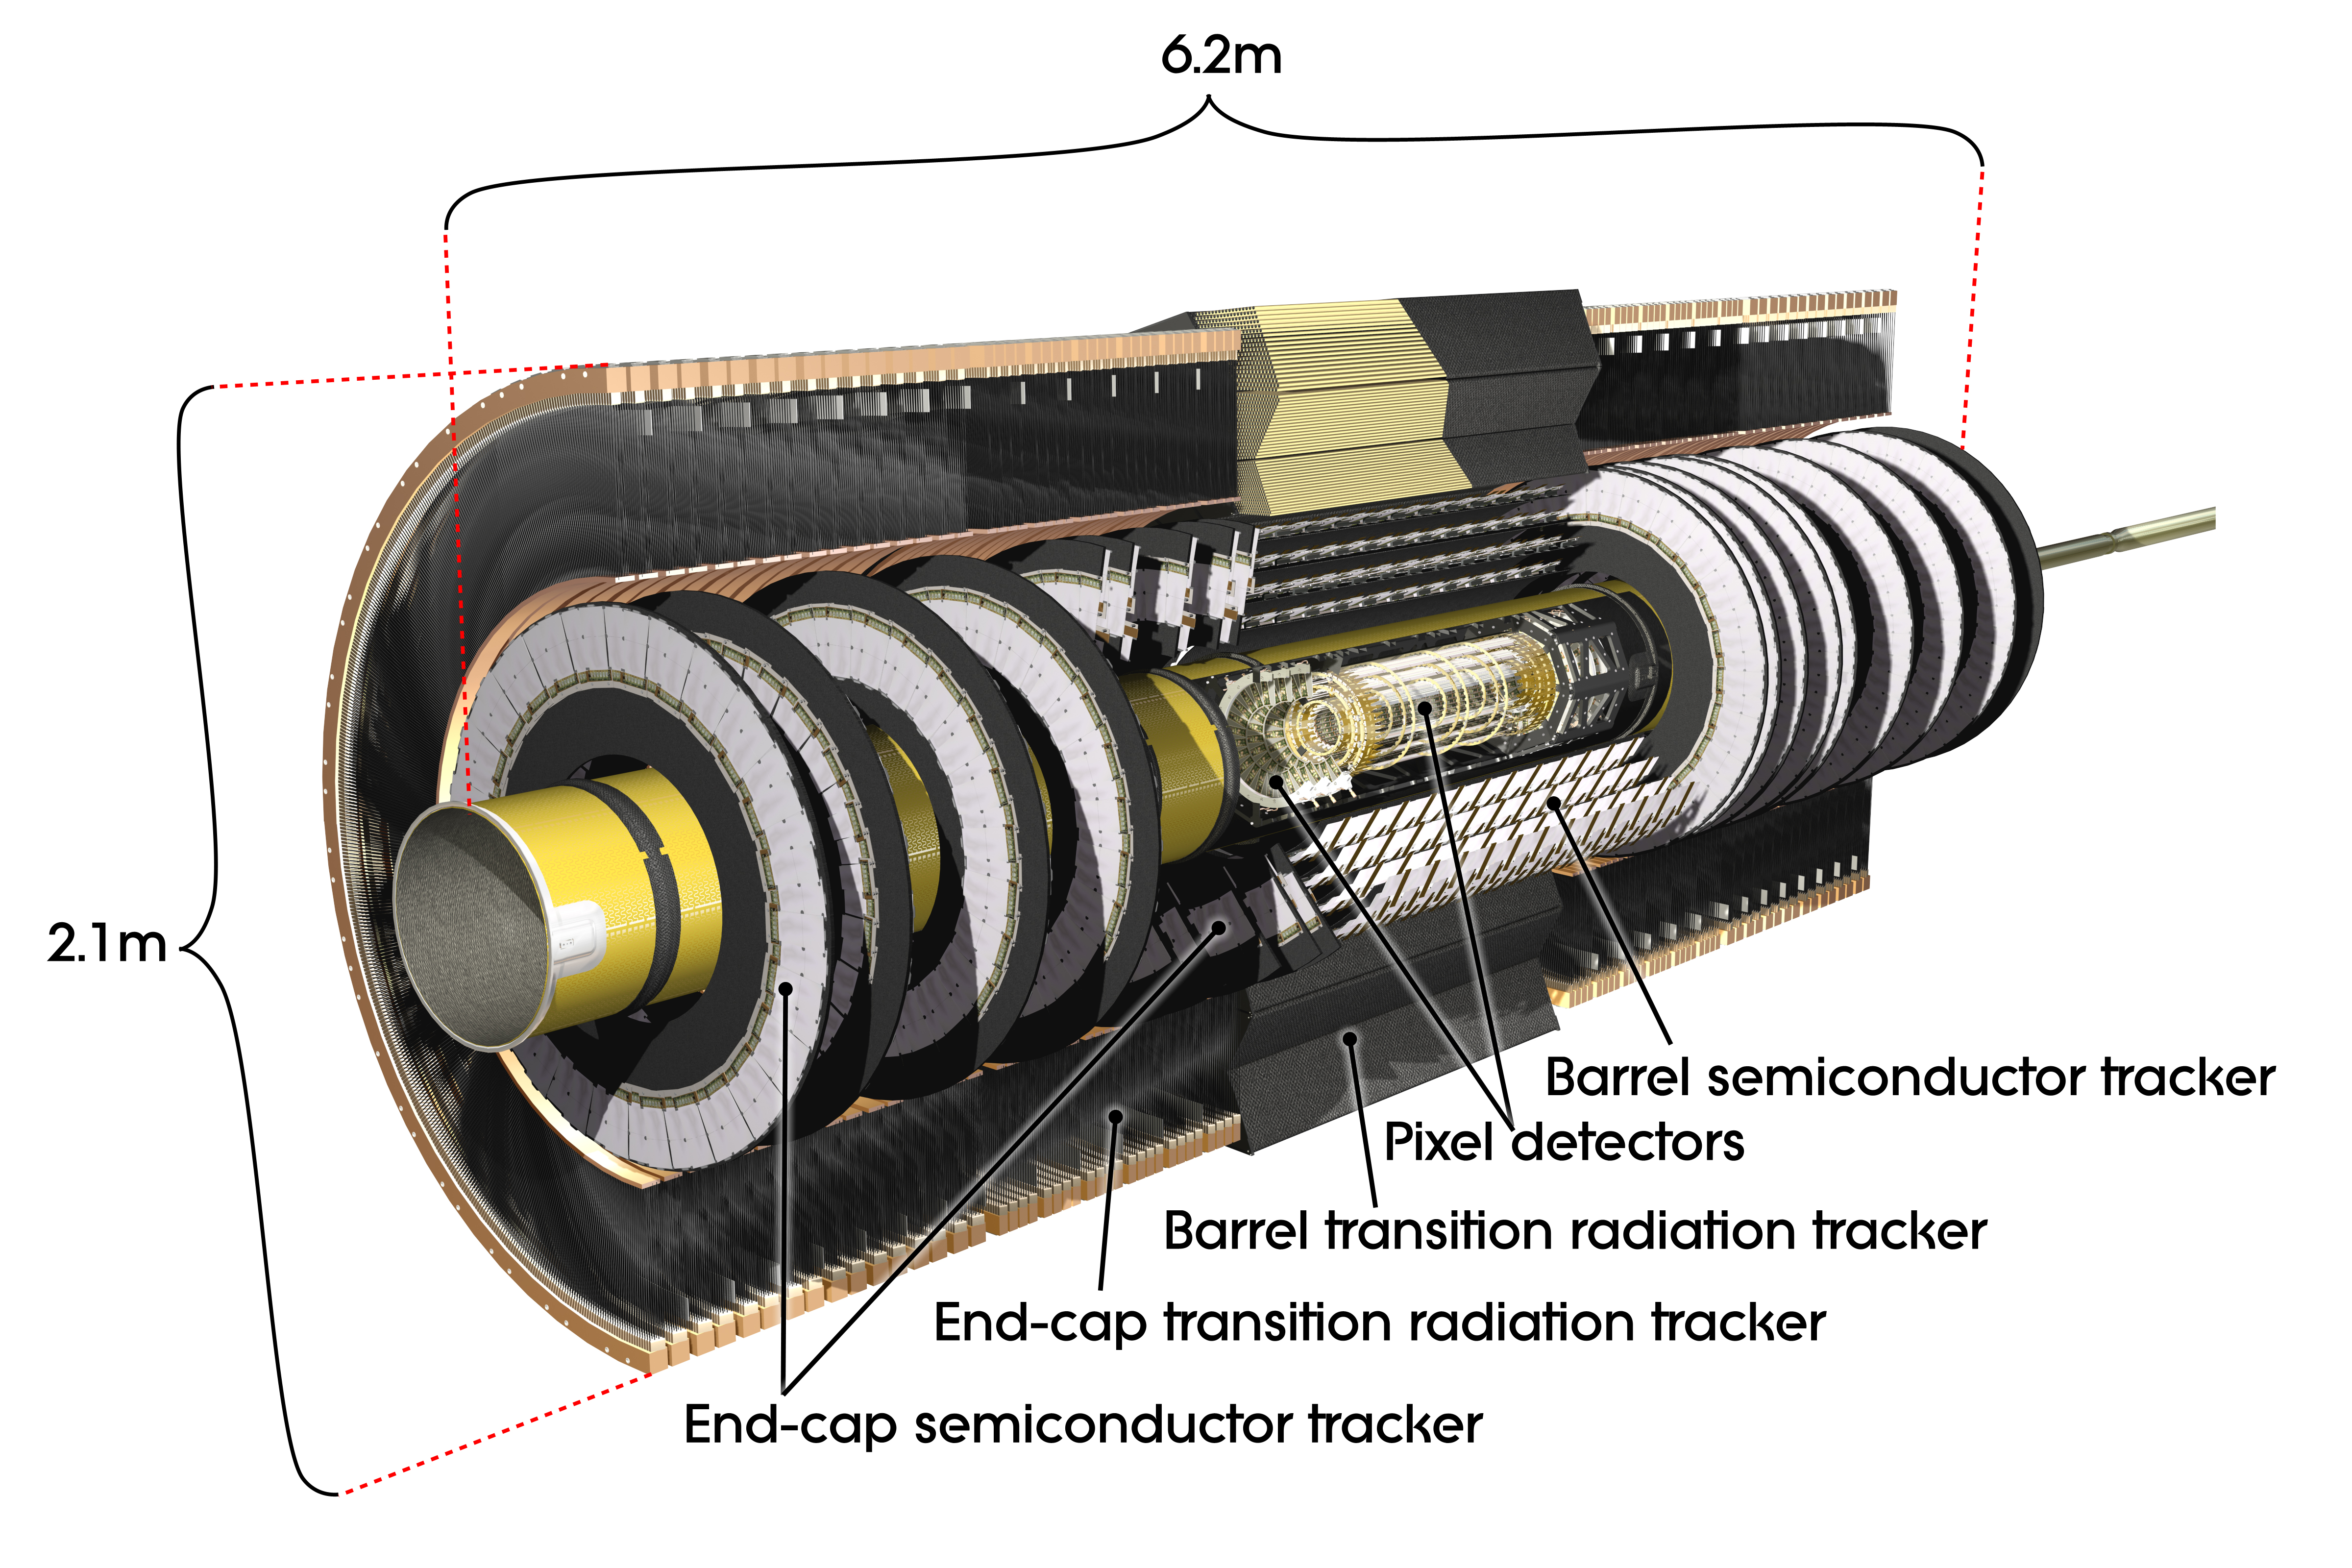
\includegraphics[width=0.7\textwidth]{Images/atlas/ID.jpg}
\caption{Cut-away view of the ATLAS Inner Detector}
\label{pic:id}
\end{figure}

\paragraph{Silicon microstrip detector}
The SCT\cite{atlas_sct} consists of four nested cylindrical barrels in the centre and nine disks in each of the two end-caps. The barrels cover a region from 300 to \SI{520}{\milli\meter} in radius and have an active length of \SI{1530}{\milli\meter}, centered around the interaction point. The respective barrel layers are fully covered by 32, 40, 48 and 56 rows of twelve identical modules, overlapping in a tile-structure in order to ensure full coverage, making a total of 2112 modules. The end-caps consist of nine disks each placed in Z at $835$ to \SI{2788}{\milli\meter} and radii ranging from 259 to \SI{560}{\milli\meter}, with the modules being placed in three rings overlapping azimuthally, two on one side, one on the other, in order to achieve full coverage.
The SCT barrel modules are made of four sensors, glued in pairs on either side of a thermally conductive baseboard. The sensors are approximately 6$\times$\SI{6}{\square\centi\meter} p-in-n silicon wafers of approximately \SI{300}{\micro\meter} thickness. Each sensor has 768 strips with \SI{80}{\micro\meter} pitch. The end-cap modules are made of two or four wedge-shaped sensors of varying size depending on their position on the end-caps rings. The strip pitch varies from \SI{57}{\micro\meter} on the inner edge of the innermost sensors to \SI{94}{\micro \meter} on the outer edge of the outermost sensors. The top and bottom sensors are rotated by a stereo angle of \SI{40}{\milli\radian} with respect each other in order to obtain two-dimensional position information while keeping the number of ghost hits small. The strips in the barrel are oriented in Z-direction and radially in the end-caps in order to obtain the best position resolution in azimuthal direction.
 The intrinsic accuracy in the barrel region is \SI{17}{\micro\meter} ($R-\phi$) and \SI{580}{\micro\meter} (z). The total number of readout channels of the SCT is approximately 6.3 million.

\paragraph{Transition radiation tracker}
The TRT\cite{atlas_trt} is composed of \SI{1.43}{\meter} long cylindrical barrel layer ranging from 56 to \SI{108}{\centi\meter} in radius and two end-caps ranging from \SIrange{0.84}{2.71}{\meter} in z and \SIrange{64}{103}{\centi\meter} in radius.
Both parts contain similar carbon-polyimide straw tubes of \SI{4}{\milli\meter} in diameter  which are aluminium-coated on theri inner surface to form a cathode and contain a gold-plated tungsten wire of \SI{30}{\micro\meter} in diameter that is used as anode. The straws are filled with 70\percent Xe, 27\percent CO$_2$ and 3\percent O$_2$, the first component being the main gas in which ionisation occurs and the latter had to be added to avoid etching problems with the glass joins that holds the wires. The straws are operated in proportional mode with the electrodes being on $\sim$\SI{1500}{\volt} bias. The 52544 straws in the barrel are \SI{144}{\centi\meter} long and formed to modules in which they are embedded in polypropylene radiator foils in which transition radiation is produced.
Relativistic particles emit transition radiation when crossing the boundary of radiator foils which is subsequently detected in the straw tubes. The signal charge from particles traversing the straws of approximately \SI{2}{\keV} is significantly lower than the signal charge created by absorption of the transition radiation photons $\sim$ \SI{10}{\keV}. Since the intensity of the emitted radiation depends on the $\gamma = E/m$ of the particle, light particles will emit more transition radiation than heavier particles which is used in the TRT to distinguish electrons from other particles such as $\pi$-mesons.
While the intrinsic resolution of the TRT cannot compete with the resolution od the silicon based technology, the high number of measurements and the long lever arm with respect to the measurements in the silicon layers makes the TRT significantly contributing to the momentum resolution. In addition, the low detector granularity is compensanted by the larger  radial positions of the straw tubes, so that a standalone pattern recognition is still possible for instantaneous luminosities up to and not beyond the nominal luminosity of \SI{e34}{\per\square\centi\meter\per\second}.

\paragraph{Impact of detector material}
\begin{figure}
\centering
\includegraphics[width=0.8\textwidth]{Images/atlas/IDMatX0.png}
\caption{Material distribution ($X_0,\lambda$) at the exit of the ID envelope, including the services and thermal enclosures. The distribution is shown as a function of $\eta$ and averaged over $\phi$. The breakdown indicates the contributions of external services and of individual sub-detectors, including services in their active volume.}
\label{fig:matbud_x0}
\end{figure}
The material budget of the tracking system must be kept to a minimum in order to limit disturbing effects form multiple scattering and not desired interactions.
%The need of a high granularity tracking detectors, in particular in the proximity of the interaction region, with related electronics, readout services and cooling, results in a relatively heavy inner detector (more than 4 tonnes), with a quite significant material budget (which can be expressed in terms of radiation lenghts $X_0$ or interaction lenghts $\lambda$).
This material has been accurately mapped and introduced in the ATLAS simulation since the impact on ATLAS performance is expected to be large:

\begin{itemize}
\item a significant fraction of low energy pions will undergo inelastic hadronic interaction inside the inner detector volume
\item approximately 40\percent of the photons convert into an electron-position pair before reaching the LAr cryostat and the electromagnetic calorimeter
\item many electrons lose a good part of their energy through bremmstrahlung before reaching the calorimeter.
\end{itemize}

The first two effects will be an important factor limiting the b-jet identification performance. This relies in fact on distinguishing higher impact parameter tracks (from b-decays) from prompt tracks.
A description of material budget can be given in term of radiation length, $X_0$. This is a characteristic of a material, related to the energy loss of high energy, electromagnetic-interacting particles with it. The definition of X$_0$ is the mean length (in \SI{}{\centi\meter}) to reduce the energy of an electron by the factor 1/e. The X$_0$ can be calculated given the characteristics of the material:
\begin{equation}
X_0=\frac{716.4 \cdot A}{Z(Z+1)ln{\frac{287}{\sqrt{Z}}}}g\cdot cm^{-2}
\end{equation}
where Z is the atomic number and A is a mass number of the nucleus.
Figure~\ref{fig:matbud_x0} shows the estimation of the $X_0$ obtained in simulation by the probability to create a photo-conversion $\gamma\rightarrow e^- e^+$ interacting with the ID material. It is a result of the need to have cooling, services and electronics inside the detector volume in order to cope with the finely granulated tracking detector elements. 

\subsubsection{Calorimeter}

The requirement of hermeticity, which is a necessary condition to achieve good resolution of the measurement of the missing transverse momentum, is one of the key design components of the ATLAS calorimeter, which in fact has a coverage up to |$\eta$| = 4.9. Different technologies are used across different regions in pseudo-rapidity as the different calorimeter sub-detectors as Figure \ref{pic:calo} shows.

\begin{figure}
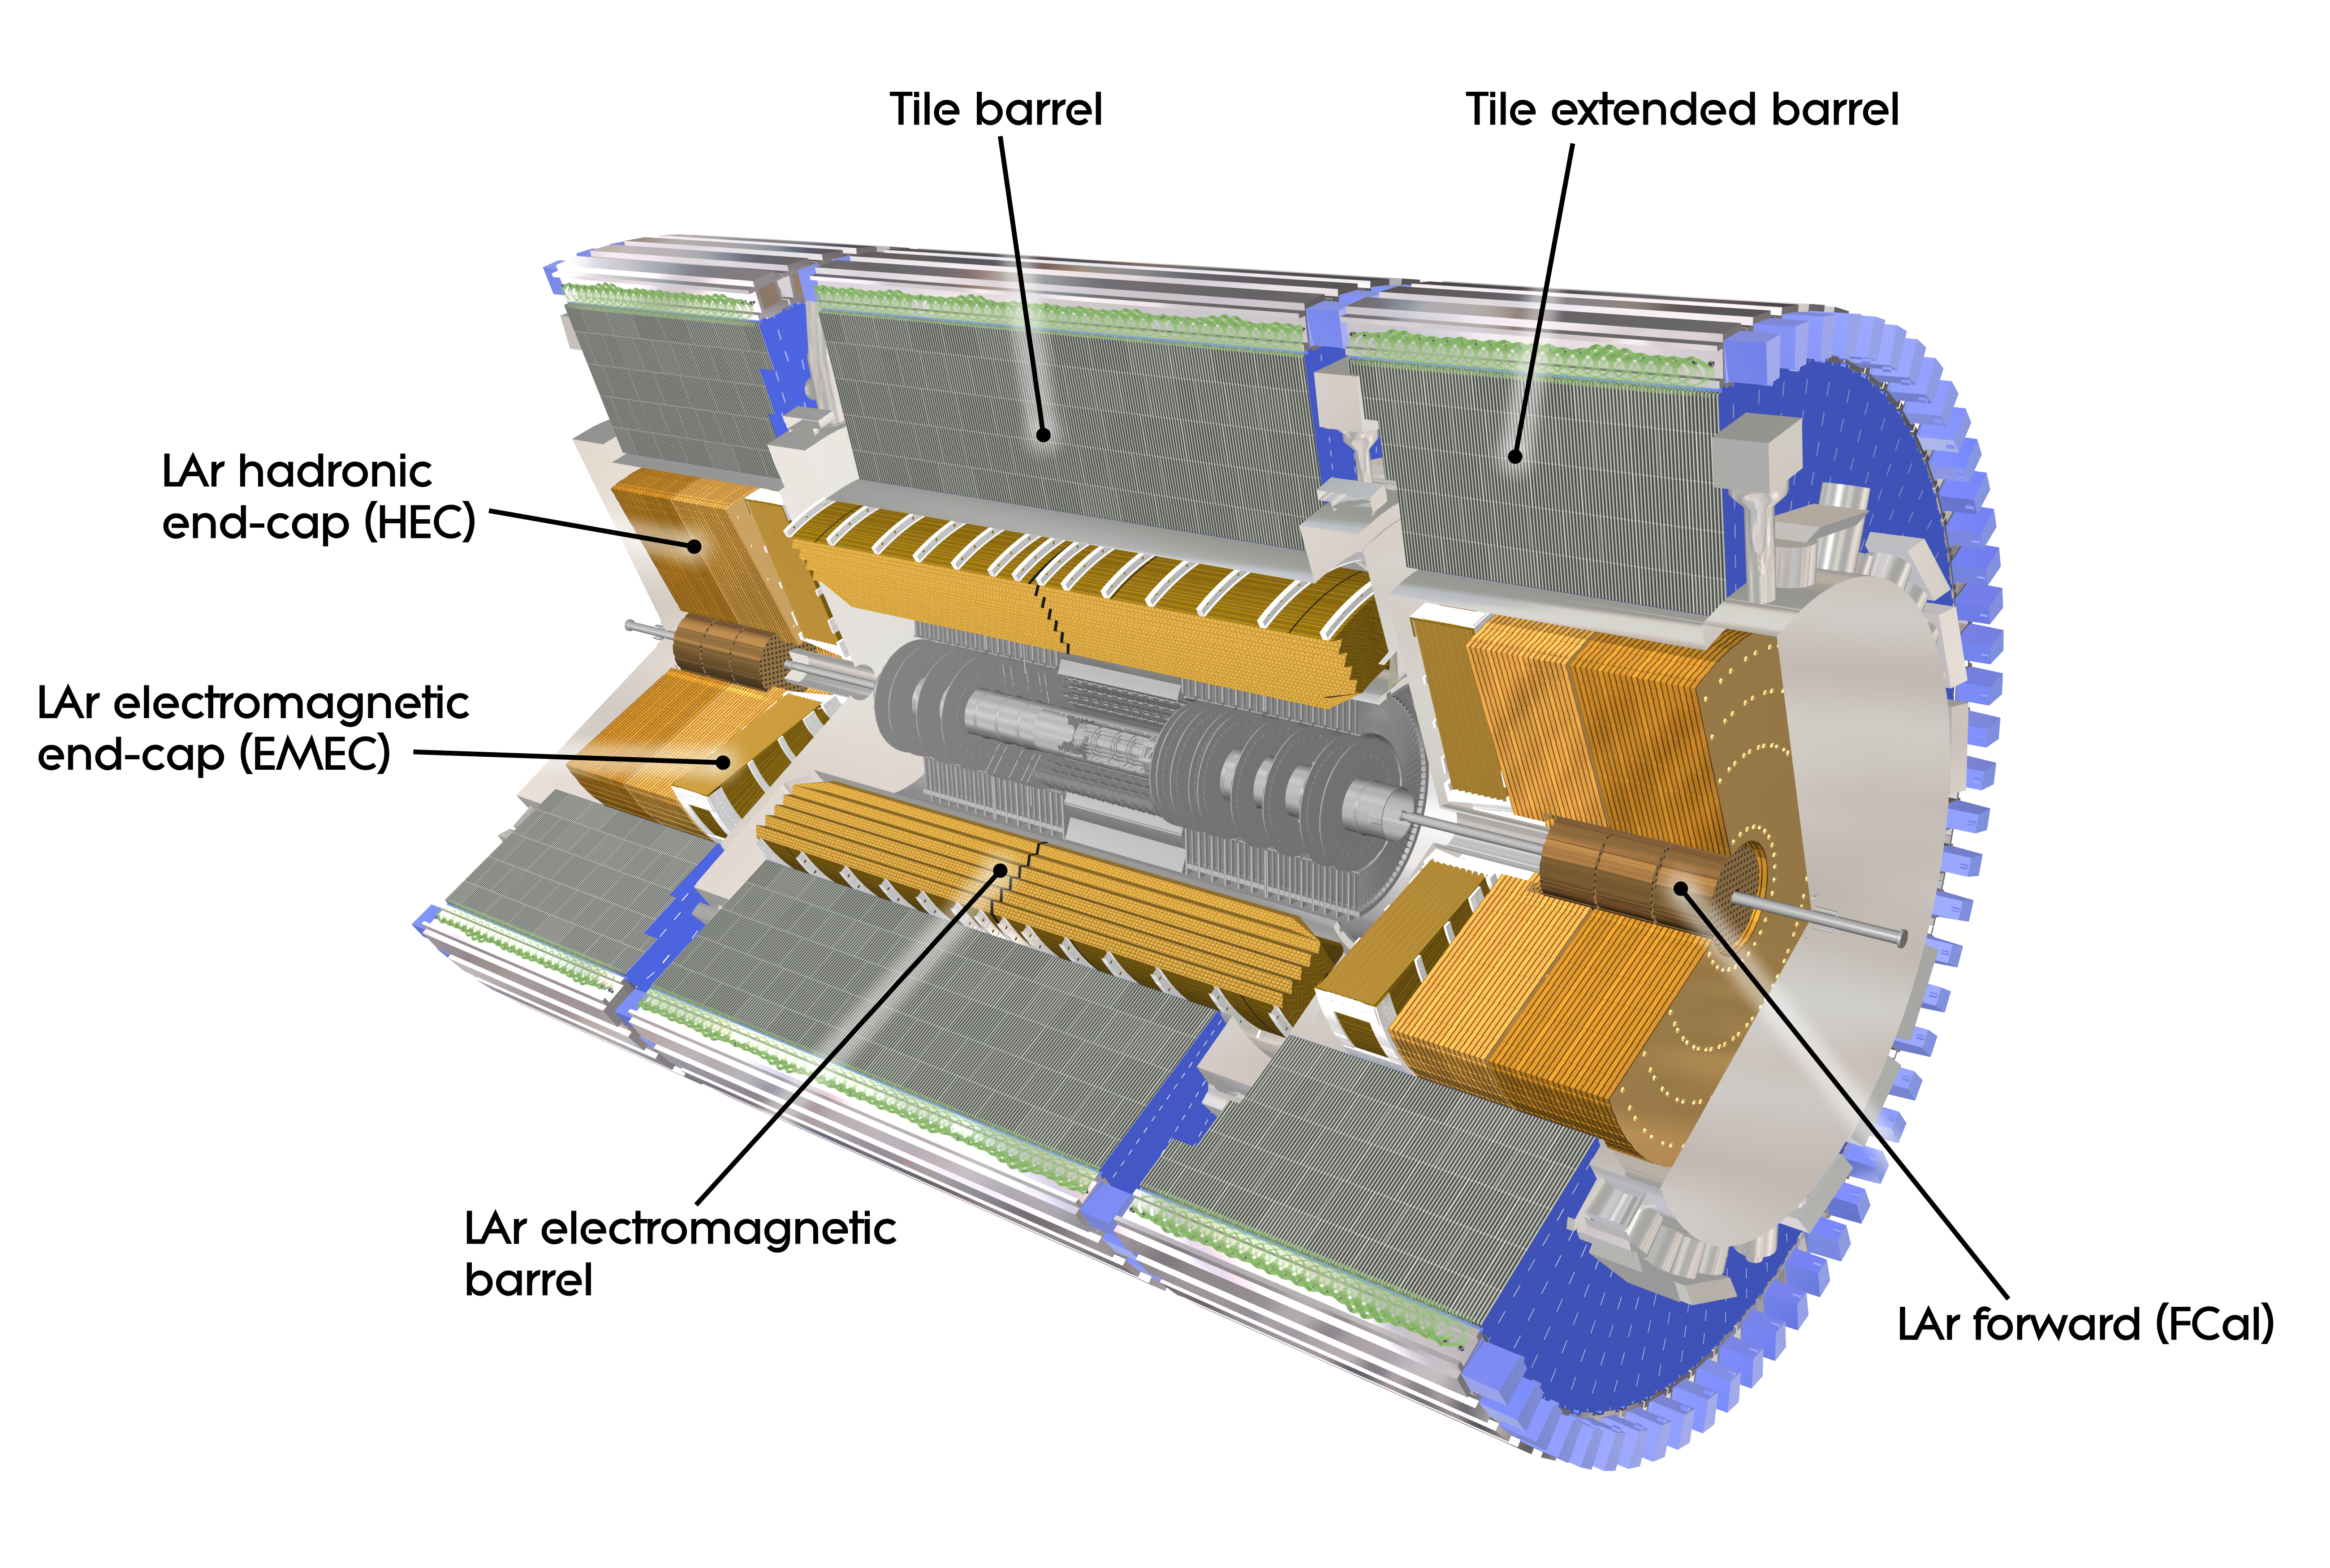
\includegraphics[width=0.8\textwidth]{Images/atlas/CALO.jpg}
\caption{Cut-away view of the ATLAS calorimeter system}
\label{pic:calo}
\end{figure}

Over the |$\eta$| range where the calorimeter is surrounding the ID, the EM calorimeter is finely segmented for precision measurements of electrons and photons, while the rest of the calorimeter is segmented more coarsely since it is mainly aimed at reconstructing jets and at measuring the missing transverse momentum.\\
Another important design criterion was the need of containing electromagnetic and hadronic showers of particles of energies around the TeV scale, since energy escaping the calorimeter results both in a significantly reduced energy resolution and in punch-through into the muon system. The total thickness of the EM calorimeter is 22~X$_0$ in the barrel and 24~X$_0$ in the end-caps.
Another important parameter to characterize the calorimeters is the absorption length $\lambda$. This is defined as distance into a material when the probability has dropped to 1/e that a particle has not been absorbed. The absorption length is typically used to describe the hadronic interaction of particles with the material.
The approximately 10 absorption length both in the barrel and in the end-caps are sufficient to provide very good resolution for high energy jets. The total thickness, including the outer support, is 11 $\lambda$ at |$\eta$|=0; this has been shown by simulation and confirmed by test beam data to be sufficient to reduce punch-throughs into the muon system well below the irreducible level of prompt or in-flight decays into muons.
The pseudo-rapidity coverage, granularity and segmentation is depth of the calorimeters are summarized in table \ref{tab:calo}

\begin{table}
\center
\begin{tabular}{l|lr|lr}
\hline
																			& \multicolumn{2}{c}{Barrel} 											& \multicolumn{2}{c}{End-cap}	\\ %				& Run II initial paramaters \\
\hline
\multicolumn{5}{c}{\tiny{EM calorimeter}} \\
\hline
\multicolumn{5}{c}{\tiny{Numbers of Layers and $|\eta|$ coverage}} \\
\hline
Presampler 													& 1 & |$\eta$| < 1.52& 2 & 1.5 < |$\eta$| < 1.8 \\
\hline
Calorimeter 												& 3 & |$\eta$| < 1.35& 2 & 1.375 < |$\eta$| < 1.5 \\
					 													& 2 & 1.35 <|$\eta$| < 1.475 & 3 & 1.5 < |$\eta$| < 2.5 \\
					 													&		&												& 2 & 2.5 < |$\eta$| < 3.2 \\
\hline
\end{tabular}
\end{table}

\paragraph{Electromagnetic Calorimeter}

The Electromagnetic Calorimeter is divided into a barrel (|$\eta$|<1.475) and two end-caps (1.375<|$\eta$|<3.2). Each end-cap calorimeter is mechanically divided in tow coaxial wheels: an outer wheel covering the region 1.375<|$\eta$|<2.5 and an inner wheel covering 2.5<|$\eta$|<3.2. The EM calorimeter is based on a lead-LAr detector with accordion-shaped kapton electrodes and lead absorbed plates over its full coverage. The liquid argon was chosen as an active medium because of its intrinsic radiation hardness and good energy resolution. he advantage of the accordion geometry is that it provides complete $\phi$ symmetry without azimuthal cracks.
Over the region which is intended to be used for precision physics (|$\eta$|<2.5) the EM calorimeter is segmented in depth in three sections. In addition, a presampler is used to recover the energy lost in dead material in front of the calorimeter. The layout of the barrel is shown in Figure \ref{pic:emcalo}.

\begin{figure}
\center
\includegraphics[width=0.8\textwidth]{Images/atlas/EMCALO.jpg}
\caption{Sketch of a barrel module where the different layers are clearly visible with the ganging electrodes in $\phi$. The granularity in $\eta$ and $\phi$ of the cells of each of the three layers of the trigger towers is also shown.}
\label{pic:emcalo}
\end{figure}

The first layer of the calorimeter, called the $\eta$-strip layer, is finely granulated in $\eta$ in order to allow for a better separation between photons (which results in a single energy deposition) and neutral pions, which results into two very close deposits of energy (from the $\pi^0\rightarrow \gamma \gamma$ decay). The resolution achievable in the barrel EM calorimeter, according to test beam data, is:

\begin{equation}
\frac{\sigma (E)}{E} = \frac{10\%}{\sqrt{E(GeV)}} \oplus 0.17\%
\end{equation}

where 10\% is the stochastic term and 0.17\% is the constant term. The energy response is also linear within $\pm0.1\%$. Similar results have been obtained for the end-cap EM calorimeters.
At the transition between the barrel and the end-cap calorimeters, at the boundary between the two cryostats, the amount od material in front of the calorimeter reaches a localized maximum of about 7$X_0$. For this reason, the region $1.37<|\eta|<1.52$ is not used for precision measurements involving photons and electrons.

\paragraph{Hadronic Calorimeters}

The hadronic calorimeters are subdivided in the tile calorimeter, whose barrel covers the region |$\eta$|<1.0 and whose extended barrels cover the region 0.8<|$\eta$|<1.7, in the LAr hadronic end-cap calorimeters, which extends from |$\eta$| = 1.5 up to |$\eta$| = 3.1 and finally the LAr forward calorimeter, which covers the pseudorapidity range up to |$\eta$| = 4.9. The tile calorimeter uses steel as the absorber and scintillating tiles as active material. Two sides of the scintillating tiles are read out by wavelength shifting fibres into two separate photomultiplier tubes. The energy response to isolated charged pions of the combined LAr and tile calorimeter was tested with test beam and turns out to be:

\begin{equation}
\frac{\sigma (E)}{E} = \frac{52\%}{\sqrt{E(GeV)}} \oplus 3\%
\end{equation}

For the end-cap hadronic calorimeters LAr technology is used, analogously to the EM calorimeter in the barrel region, but copper is used instead of lead as a passive material and a flat-late geometry was chosen. The energy response to isolated pions can be condensed in the energy resolution:

\begin{equation}
\frac{\sigma (E)}{E} = \frac{71\%}{\sqrt{E(GeV)}} \oplus 1.5\%
\end{equation}

Finally, the forward calorimeter is based again on LAr active material and uses copper as passive absorber material for the first layer and tungsten for the second and third layer. As a result of test beam data the energy response to pions is expressed by the relative energy resolution:

\begin{equation}
\frac{\sigma (E)}{E} = \frac{94\%}{\sqrt{E(GeV)}} \oplus 7.5\%
\end{equation}



\subsubsection{Muon System}

The detection of muons in ATLAS can count on a dedicated sub-detector. Muons are among the most important signatures for interesting processes at the LHC and have a clear advantage that they are the only charged particles which are not stopped in the calorimeter (apart rare cases of punch-through) and they are detected in the muon system. This can be exploited also for the on-line selection of events.
The muon detector is based on two kind of sub-detectors, one for precision measurements, which is needed to determine the muon momenta with high precision, and another for the online trigger of muon events, which requires very fast sub-detectors and are needed to uniquely associate the muons to a certain bunch crossing. The precision measurements are performed by the Monitored Drift Tube chambers (MDT), which cover the pseudorapidity region up to 2.7, and, in the forward region (2<|$\eta$|<2.7), by Cathode-Strip Chambers (CSC), which are used in the innermost layer due to their capability of working at high rate and better time resolution.
The MDT chambers only constrain the muon track in the bending plane (z-coordinates), with a precision of \SI{35}{\micro\meter}, while the CSC, being multi-wire proportional chambers with cathode planes segmented into strips in orthogonal direction, provide a measurement both in the R direction of \SI{40}{\micro \meter} precision and in the $\phi$ direction of \SI{10}{\milli\meter}.
These chambers are complemented (both for the measurement of the missing $\phi$ in case of the MDT and for the online event selection) in the barrel region (|$\eta$|<1.05) by Resistive Plate Chamber (RPC) and in the end-cap (1.05<|$\eta$|<2.4) by Thin Gap Chambers (TGC). The intrinsic time resolution of these detectors components (\SI{1.5}{\nano\second} for RPC and \SI{4}{\nano\second} for TGC) is appropriate for triggering and permits to identify the correct bunch crossing.\\
Given the three chambers layout of the muon system, the momentum measured of a high-\pt track will depend on the resolution by which its sagitta (determined in the R-z plane in the middle chamber with respect to a straight line) can be determined. For high-pt track of \SI{1}{\TeV}, this sagitta will be about the \SI{500}{\micro \meter}. The muon chamber resolution provided in $\phi$ by the MDT chambers allows to reach a precision better than 10\% in the momentum measurements of muons up to \SI{1}{\TeV}, which corresponds to the design goals of ATLAS.
For the measurements of low-\pt muons, the measurements in the muon system typically need to be complemented by measurements in the ID, since in general not all muon stations will be reached due to the stronger bending of low-\pt particles in the magnetic field.

\subsubsection{Trigger System}

The ATLAS experiment uses a two staged trigger system to identify collisions events of interest.\\
The first stage, called Level-1 trigger, reduces the event rate from \SI{40}{\mega\hertz} to \SI{100}{\kilo\hertz},
since a decision must be taken every \SI{25}{\nano\second}. Since the transit and processing time of around \SI{2.5}{\micro\meter}, the detector data must be time stamped and held in the buffers of the front-end circuit.
The Level-1 trigger uses information from dedicated muon trigger and from the calorimeters. The only signatures which can be selected in the L1 trigger are high-\pt muons, electrons/photons, jets, $\tau$-lepton decaying into hadrons and missing transverse energy. No information coming from the tracking devices can be used at L1, so, for example, it is not possible to select b-jets at this level.\\
The second stage of the trigger system reduces the event rate further \SIrange{0.5}{1}{\kilo\hertz}. It is software based and uses offline-like reconstruction algorithms, utilizing informations from all sub-detectors in regions of interest around the Level-1 objects in full granularity. The regions of interest are areas of the detector which the L1 trigger has identified as interesting. The use of regions of interest allows to have a fast execution time keeping high the selection efficiency.

%The L2 and EF triggers form the High-Level Trigger (HLT) and are both based on commercially available computer and networking hardware. The main difference between the L2 and the EF is that the first is seeded by so-called Regions-of-Interests (RoI), which are regions of the detector which the L1 trigger has identified as interesting, while the second is based on full-detector-granularity. In this way the L2 trigger is much quicker and yields a first rate reduction from $75~kHz$ to below $3.5~kHz$, with an average processing time of approximately $40~ms$, while the EF brings this further down to $200~Hz$, with a processing time per event of around 4 seconds. The higher granularity, tracking information and improved reconstruction make a refined decision with respect to the L1 possible. The final rate can be sustained by actual storage technology.

\subsection{The LHC upgrade program}

\begin{figure}
\center
\subfloat[2011 Luminosity]{\label{pic:atlaslumi2011}\includegraphics[width=0.45\textwidth]{Images/atlas/ATLASLUMIRUN1_2011.png}}\quad
\subfloat[2012 Luminosity]{\label{pic:atlaslumi2012}\includegraphics[width=0.45\textwidth]{Images/atlas/ATLASLUMIRUN1_2012.png}}
\caption{Cumulative luminosity versus day, in green the amount of luminosity deliverd to ATLAS and in yellow the recorderd one. This assume stable beam configuration for proton-proton collisions.}
\label{pic:atlaslumi}
\end{figure}
The LHC machine and the related experiments showed excellent performance in the first run period of the LHC, which took place in between 2010 and 2012, delivering almost \SI{30}{\per\femto\barn} to the ATLAS and CMS experiments. The ATLAS experiment was able to record 93$\percent$ of the delivered luminosity as shown in Figure \ref{pic:atlaslumi} for what concerns the proton-proton collisions.

\begin{figure}
\center
\includegraphics[width=0.9\textwidth]{Images/atlas/ATLASSM.png}
\caption{Detailed summary of several Standard Model total production cross section measurements, corrected for leptonic branching fractions, compared to the corresponding theoretical expectations. All theoretical expectations were calculated at NLO or higher. The W and Z vector-boson inclusive cross sections were measured with \SI{35}{\per\pico\barn} of integrated luminosity from the 2010 dataset. All other measurements were performed using the 2011 dataset or the 2012 dataset. The dark-color error bar represents the statistical uncertainly. The lighter-color error bar represents the full uncertainty, including systematics and luminosity uncertainties.}% The data/theory ratio, luminosity used and reference for each measurement are also shown. Uncertainties for the theoretical predictions are quoted from the original ATLAS papers. They were not always evaluated using the same prescriptions for PDFs and scales. For the dijets measurement, $y^* = |y_1 - y_2|/2$, where $y_i$ is the jet rapidity. }
\label{pic:atlassm}
\end{figure}

Detailed measurements of well-known SM processes were performed and used to calibrate the detector. Figure \ref{pic:atlassm} shows the measured production cross section for several SM processes with their theoretical prediction. 
The success of the discovery of the Higgs Boson was just one of the impressive results achieved by LHC experiments during the first period of data-taking. Further investigation on the Higgs boson properties and in the search of new physics phenomena will require to collect more data; therefore the LHC luminosity need to increase and the detectors performance need to improve. An increase of the center of mass energy will allow to explore a more wide phase space of physics phenomena.\\
\begin{figure}
\centering
\includegraphics[width=0.9\textwidth]{Images/atlas/LHC_upgrade_program.png}
\caption{Time schedule for the long LHC shutdowns and the run phases}
\label{pic:lhc_schedule}
\end{figure}
Figure~\ref{pic:lhc_schedule} summarizes the upgrade steps of the LHC machine. A first long shutdown happened from February 2013 to April 2015 to consolidate the magnet inter-connects of the LHC machine. This upgrade was needed to run the LHC at the design energy of \SI{7}{\TeV} per beam and at the design luminosity of \SI{e34}{\per\square\centi\meter\per\second}. The period after such an upgrade of the LHC is usually referred as Run 2, and it should last from 2015 to 2019, aiming to collect \SI{100}{\per\femto\barn} of data. The Run 2 has began in the spring of 2015, with a \SI{13}{\TeV} center of mass energy, which will be upgraded to \SI{14}{\TeV} in next years.
A second and a third shutdown with machine development are foreseen in 2019 and 2024, where the luminosity should be upgraded to twice and five times the nominal value.
The LHC plan is to record about \SI{3000}{\per\femto\barn} during the entire LHC data-taking campaign.\\
The LHC upgrades provide the opportunity to upgrade the experiments and to recover possible failures.
The first long shutdown was used for an upgrade of the ATLAS pixel detector as it will be discussed in Chapter 3 of this thesis. While no upgrade of the ATLAS Pixel detector is foreseen in the second long shutdown a complete redesign will be needed after the third long shutdown. The new system should in particular sustain the harsh radiation environment and provide fast information for the new track based trigger system.
%\subsection{Physics with b-tagging in the LHC Run 2}
%The identification of jets containing b hadrons is an important tool used in a spectrum of measurements comprising the Large Hadron Collider (LHC) physics programme. In precision measurements in the top quark sector as well as in the search for the Higgs boson and new phenomena, the suppression of background processes that contain predominantly light-flavour jets using b-tagging is of great use. It may also become critical to achieve an understanding of the flavour structure of any new physics (e.g. supersymmetry) revealed at the LHC.
%Several algorithms to identify jets containing b hadrons have been developed, exploiting the
%long lifetime, high mass and decay multiplicity of b hadrons and the hard b-quark fragmentation
%function. They range from an algorithm that uses the signed significance of the decay length with
%respect to the proton-proton collision location, in the following referred to as the primary vertex,
%of an inclusively reconstructed secondary vertex to more refined algorithms using both secondary
%vertex properties and the significance of the transverse and longitudinal impact parameters of the
%charged particle tracks. The most discriminating variables resulting from these algorithms are
%combined in artificial neural networks. An independent b-tagging algorithm based on reconstructed
%muons inside jets, exploiting the relatively large fraction of b-hadron decays with muons in the
%final state, about $20\percent$, and the b-tagging algorithm used for the online trigger selection are also used.
%The performance of the tagging algorithms is studied in simulated events, including the dependence on additional proton-proton interactions in the same bunch crossing, referred to as pile-up.


\pagebreak

\section{Track reconstruction with pixel detectors}\label{sec:Tracking with pixel}
%\pagestyle{plain}
Precise tracking is a fundamental tool for any collider experiment. An efficient identification of electrons and muons, based on tracking, is a key factor for a correct reconstruction of the final states of collisions events.\\
It is important to determine the position of the interaction point, the primary vertex, moreover some particles do not decay promptly after the production and they neither live enough to transverse the full detector, i.e. hadrons containing b and c-quarks and the $\tau$-lepton.
%Hadrons composed of a b or c quark and a lighter quarks (as $D^0$ and $B^0$), have a lifetime dominated by the decay of the heavier quark, which is mediated via the weak interaction. The life-time at rest of these particles is of the order of magnitude of the \SI{}{\pico\second}.
%The $\tau$-lepton has a rather large mass compared to the other two charged leptons and a lifetime $\tau_{rest} = \SI{290}{\femto\second}$\cite{tau_life}.
All these particles have in common that they decay inside or close to the innermost detector layer, but on average live long enough to have their decay detected by measuring the position of their decay vertex, the secondary vertex.\\
% Particles produced in high-energy experiment are usually highly relativistic. Since the life-time of a boosted particle is  $\tau_{boosted} =\gamma \tau_{rest}$, the secondary vertex will be displaced from the primary vertex, the secondary vertex can be then measured and identified, i.e. a $\tau$-lepton of \SI{100}{\GeV} momentum extend travels for $\sim$\SI{5}{\milli\meter} in average.\\
Pixel detectors play a fundamental role in tracking and vertex identification thanks to their high density of readout channel, good time resolution and the high radiation hardness.
The high density of channel lead to a high spatial resolution, this feature is extremely important for being able to distinguish each of the tracks in dense environment, so that pixel detectors can be used for pattern recognition purposes.
The high rate of collision of LHC requires also detectors to be very fast, and operate at the typical \SI{40}{\mega\hertz} rate. Pixel detectors meet this requirement thanks to fast transistors with dimension of the order of \SI{200}{\nano\meter}. This detection technique is ideal for operating close to the IP due to its radiation hardness performance.
%The radiation hardness performance of silicon devices, used both as front-end readout and detective bulk, makes pixel detector ideal candidates for operating close to the IP of particle physics experiment.
%Their tracks are superimposed on those produced in the rare high-\pt collisions leading to very complex patterns that can be reconstructed efficiently only by high granularity devices with good time resolution.
%At the \TeV-scale the pattern recognition has the additional challenge of precisely reconstructing the tracks of narrow jets produced by highly boosted low mass particles like highly energetic b-jets.\\
In this chapter the mechanism of charged particles detection, tracking in magnetic field and vertices discrimination will be covered.
\subsection{Particle interaction with matter}
A particle could interact with the material that is crossing through either losing some of its own energy or deflecting its trajectory. Those property are used to detect particle flow in the particle detectors.
The energy loss could happen either via electromagnetic or nuclear interactions, involving the atom's electrons and nuclei.
Particles detectors are mainly distinguished by the mechanism they use to reveal the particles and the type of particles they are devoted to detect, i.e. tracking detectors normally detects charged particles via ionization interaction.
In this section a brief description of the main interaction processes in tracking detectors will be presented.
%Particles interact with matter through several processes that depends on the characteristichs of the particles themselves and of the material that they cross.


\subsubsection{Interaction of charged particles}
The description of the energy loss of a charged particle through ionization phenomena is provided by the Bethe-Block formula\cite{bethe_block}, a quantum-mechanical correction to the Bohr formula which uses a classical electro-dynamic approach.
The mean energy loss per lenght $<\frac{dE}{dx}>$ is:
\begin{equation}
-<\frac{dE}{dx}>~=~\frac{4\pi r^2_e m_ec^2 N_A Zz^2 \rho}{A\beta^2}\bigg( \frac{1}{2} ln\bigg( \frac{2m_e c^2 \beta^2 \gamma^2 T_{max}}{I^2}-\beta^2 -\frac{\delta(\beta \gamma)}{2} \bigg) - \frac{C}{Z}  \bigg)
\end{equation}
where $Z$ and $A$ are the atomic and the mass number of the material, $\rho$ is the material density, $N_A$ is the Avogadro constant and $r_e=\SI{2.8}{\femto\meter}$ is the classical electron radius, $z$ is the charge of the incident particle in unity of electrons, $\beta = \frac{v}{c}$ and $\gamma = \frac{1}{\sqrt{1-\beta^2}}$, where $c$ is the speed of light. The mean excitation energy of the material $I\simeq I_0Z$ with $I_0 \simeq 12 \eV$ when $Z<13$. $T_{max}$ is the maximum kinetic energy which can be imparted to a free electron in a single collision. C is the shell correction.
The density correction $\delta$ is an effect which becomes important at high energy, the incident particle is polarizing the material while crossing it. This produces a shield effect on atoms far from the particle, reducing the energy loss.
\begin{figure}
\center
\includegraphics[width=0.6\textwidth]{./Images/tracking_det/BetheBlock.png}
\caption{The Bethe-Bloch equation solved for numerous materials in case of a single charge particle.}
\label{pic:bethe}
\end{figure}
As a function of $\beta \gamma$ the energy loss has no dependency on the mass of the incident particle. The Bethe-Block formula is valid in the $\beta \gamma$ range from 0.05 and 500, outside this range other processes than ionization are dominant.\\
Figure \ref{pic:bethe} shows the mean energy loss of a particle crossing a material as a function of its $\beta \gamma$.
Due to the small increase above the minimum, all the particles with $\beta \gamma~>~3$ are commonly called Minimum Ionizing Particles. This condition is typical of the collision products of the LHC.
The calculation of energy loss depends on the width of the absorber media. For thick absorber the distribution of energy loss is gaussian, given the high number of interactions. For thin absorber the number of interaction is low and the energy loss distribution is not gaussian. A theoretical calculation was provided by Landau\cite{landau}, Symon and Vavilov based on the parameter $\kappa = \frac{\overline{\Delta}}{W_{max}}$, where $\overline{\Delta}$ is mean energy transferred in a single scattering and $W_{max}$ is the maximum energy that can be trasferred in a single scattering process.
The Landau theory is valid for $\kappa \le 0.01$ and it assumes that $W_{max}\rightarrow \infty$, the trasferred energy is high enough that the electrons could be considered as free, the speed of the incident particle remains constant in the scattering process. The integral transport equation can be solved under these hypothesis.
\begin{equation}
\frac{df}{dx}(x,\Delta) = \int_0^{\infty}W(E)[f(x,\Delta - E)-f(x,\Delta)]\mathrm{d}E
\end{equation}
Here $f(x,\Delta)$ represents the distribution probability that the incident particle will lose an amount $\Delta$ of energy on traversing a layer of thickness x. $W(E)dE$ denotes the probability per unit path length of a collision transferring energy E to an electron in the material. The function $W(E)dE$ is not generally known, an approximate solution by using the free electron (Rutherford) cross section that matches with the hypothesis:
\begin{equation}
W(E) = \frac{\xi}{x} \frac{1}{E^2} \quad \& \quad \frac{\xi}{x}=0.1535\frac{z^2 Z \rho}{A \beta^2 } 
\end{equation}
The Landau distribution is therefore given by:
\begin{equation}
\begin{split}
f_L(x,\Delta) = \frac{\phi(\lambda)}{\xi}\quad \& \quad \phi(\lambda) = \frac{1}{\pi} \int_0^{\infty}e^{ -t \mathrm{ln}(t) -\lambda t  } sin(\pi t) \mathrm{d}t 
\\
\lambda = \frac{\Delta -\overline(\Delta)}{\overline{\Delta}} -\mathrm{ln}(\frac{\overline{\Delta} 2mc^2 \beta^2}{(1-\beta^2)I^2})- 1 +C_E
\end{split}
\end{equation}
where $C_E=0.5772$ is the Eulero constant.
The Landau distribution, $f_L(x,\Delta)$, is asymmetric with a tail extending to $E_{max}$. This tail is mainly due to fast emitted $\delta$-rays, electrons with enough energy to escape a significant distance away from the primary radiation beam and produce further ionization. The energy loss corresponding to the maximum of the function $f_L(x,\Delta)$ is the most probable energy loss.
\begin{figure}
\center
\includegraphics[width=0.6\textwidth,height=0.45\textwidth]{Images/tracking_det/Landau.jpg}
\caption{Landau functions in silicon for 500~MeV pions, normalized to unity at the most probable value $\Delta_p/x$. The Landau distribution is shown for different widths of silicon layers.}
\label{pic:landau}
\end{figure}
Figure \ref{pic:landau} shows the typical Landau distribution for different widths of silicon layers for an incoming 500~\MeV pion.
%dSeveral mechanisms describe the energy loss of a particle into the material: ionization of the atoms of the material, emission of Cherenkov radiation, emission of transition radiation, bremmsstrahlung processes and nuclear reactions. The first three are electromagnetic processesand they are dominant for particles with low momentum.
\subsubsection{Particle scattering}
In addition to inelastic collisions with the atomic electrons, particles passing through matter undergo repeated elastic Coulomb scattering from nuclei although with a smaller probability.
Considering that usually nuclei have mass greater than the incoming particle, the energy transfer is negligible but each scattering centre adds a small deviation to the incoming particle's trajectory also. Even if this deflection is small, the sum of all the contribution adds a random component to the particles path which proceed with a zig-zag path. As result, particles show a deviation from the incoming trajectory after having crossed a material.
Three possibility can be considered:
\begin{itemize}
\item Single scattering. When the thickness is extremely small and the probability to have more than one interaction is negligible. In this case the situation is well described by Rutherford formula\cite{rutherford}: 
\begin{equation}
\frac{d\sigma}{d\Omega} = \big(\frac{1}{4\pi\epsilon_0} \big) \frac{ z_1^2 z_2^2 e^4}{M^2c^4\beta^4} \frac{1}{sin^4(\frac{\theta}{2})}
\end{equation}
\item	Plural scattering. When the number of Coulomb scattering increases but remains under few tens of interactions. This is the most difficult case to deal with, several works have been done by different authors\cite{plural_scattering}.
\item Multiple scattering\cite{multiple_scattering}. When the thickness increases and the number of interactions become high the angular dispersion can be modeled as Gaussian.
\end{itemize}
Multiple scattering is the most common situation. The angular dispersion can be calculated as:
\begin{equation}
\sigma_{\Theta_0} = \frac{13.6 MeV}{\beta c p}z \sqrt{\frac{x}{X_0}}[1+0.038\mathrm{ln}(\frac{x}{X_0})]
\label{eq:mult_scat}
\end{equation}
where p is the momentum, z is the charge of the incident particle and $\frac{x}{X_0}$ is path in radiation length in the absorber material.
% The standard deviation $\sigma_0$ of this distribution depdends on the radiation lenght $X_0$ of the material, the momentum $p$, a
Multiple scattering contributes to the uncertainty on the track reconstruction. Reducing the detector thickness and using material with larger $X_0$ decrease the standard deviation of the scattering angle distribution.
\subsubsection{Interaction of neutral particles}
Charged particles are not the only one contributing to energy release in the matters, also release of energy from neutral radiation needs to be considered.
Significant contributions come from photons and from neutral hadrons as neutrons. The two type of particles interact in a very different way and have different impact on tracking performance.
Photons can interact in many ways with the material via electromagnetic interactions. The type of interaction depends on the atomic number of the material Z and of the energy of the photons themselves.
\begin{figure}
\center
\includegraphics[width=0.5\textwidth]{Images/tracking_det/photon_interaction.png}
\caption{Mass attenuation coefficient of the silicon and its components.}
\label{pic:photon_interaction}
\end{figure}
Figure \ref{pic:photon_interaction} shows the mass attenuation coefficient of photons in silicon and the contribution from different processes. Mass attenuation coefficient characterizes how easily a material can be penetrated by a beam and it is defined as $\frac{\mu_a + \mu_s}{\rho}$, where $\mu_a$ is the absorption coefficient, $\mu_s$ is the scattering coefficient and $\rho$ the material density. Several types of photon interaction with matter are possible, the most probable are:
\begin{itemize}
\item Photoelectric effect: which is the most probable interaction for energy lower than \SI{0.1}{\MeV}
\item Compton effect: which is the most probable interaction in the energy range \SIrange{0.1}{100}{\MeV}
\item Pair production via bremsstrahlung: which is the most probable interaction for energy higher than \SI{100}{\MeV}
\end{itemize}
%While photoelectric absorption and Compton effect are dominant at low photon energy ($E_{\gamma}<\SI{100}{\MeV}$), at high energy the dominant process is the pair production via bremsstrahlung. 
In the LHC environment photons are typically high energetic and the pair production mechanism is the dominant one and it will be taken in consideration in the following text.
Although pair production is the key-process for photon identification in the calorimetry, it is a background phenomenon that could lead to fake reconstructed tracks and vertices in the Inner Detector.
In this process the photon interacts with an electron or a nucleus producing a positron-electron pair. In order to produce the pair the photon must have at least an energy of 1.022\MeV. In Figure~\ref{pic:photon_interaction} the two components of the pair production cross section are shown, respectively for the interaction with nuclei or electrons.\\
Neutron can interact with matter by strong interaction with nuclei. In general strong interaction could happen also with charged hadrons, as protons, but it is rare with respect to electromagnetic interaction, though, with the high fluences of LHC it needs to be well monitored and described because of the radiation damage that will cause.
For a strong interaction to happen the hadron needs to be at $\simeq$~\SI{10}{fm} from the nucleus. The type of neutron interaction will depend upon the energy of the neutron and the mass number of the material itself, here a list of the most important phenomena:
\begin{itemize}
\item Elastic scattering, which is dominant in the MeV region;
\item Inelastic scattering, in which the nucleus is excited and then decays with the production of $\gamma$. This phenomenon has a energy threshold of about 1~\MeV;
\item Neutron capture, corresponding to the process $n+(Z,A)\rightarrow \gamma + (Z,A+1)$, which is dominant for low energy neutrons (\eV-\keV);
\item Other nuclear reactions, which typically happen for low energy neutrons (\eV -\keV);
\item Production of hadronic showers, for very high energy neutrons ($\simeq$~100~\MeV)
\end{itemize}
The cross section of neutron interaction is proportional to the velocity of the neutron itself, as $1/v_n$, this means that the most interacting neutrons are the low energetic ones, which are then the most dangerous one for devices that needs to operate in a radioactive environment. Details about the radiation damage will be treated later in this thesis work.
% Another possible interaction, but usually negligible compared to the previous ones is the Photonuclear reaction, in this case the photon interact directly with the nucleus. The related cross section is shown in Figure 1 in dotted line (σg.d.r.). 
%A suitable quantity, often used to characterize the absorption of a photon shower, is the mass attenuation coefficient. The mass attenuation coefficient is defined as:
%\begin{equation}
%\mu_m = \eta_A \frac{\sigma_{tot}}{\rho}
%\end{equation} 
%where 

\subsection{Properties of pixel silicon detector}
\begin{figure}
\centering
\includegraphics[width=0.4\textwidth]{Images/tracking_det/hybrid.png}
\caption{Cross section of hybrid pixel readout channel. Sensor, at the bottom, provides the signal generation, the bump, in the middle, provides the interconnection and the readout chip, at the top, takes care of the signal amplification and the data processing.}
\end{figure}

The main tasks of the pixel detector is the pattern recognition and the measurement of momentum for charged tracks. Additionally pixel detectors contribute to the resolution of the secondary vertices from the primary vertex. Pixel detectors are made of silicon sensors. The choice of silicon as a bulk material is motivated by the radiation hardness performance, the possibility to achieve a fine segmentation, the good time resolution and the high availability which drives the relatively low cost.
A brief description of the main properties and the most important aspects that need to be consider in silicon detectors follows.\\
There are two possible option for pixel silicon sensors, either the readout electronics is integrated on the sensor itself (monolithic sensor) or the readout electronic is integrated in an external chip, connected to each pixel of the sensor (hybrid sensor). Radiation hard design of the silicon sensor typically requires the use of high voltage bias, so that a radiation hard monolithic sensors is possible only if the electronics is well protected from the bias applied to the bulk, as it is possible using the HVCMOS technology. The use of HVCMOS technology is currently investigation and it was not considered for the construction of the ATLAS pixel silicon sensors, whose approach was the use of hybrid sensors.\\
The working principle of hybrid sensors is shown in Figure~\ref{fig:hybrid}, the signal is created in the silicon sensor and then transmitted to the readout chip connected to the sensor via a metallic bump.

\subsubsection{Signal generation in silicon sensors}

%An ionizing particle crossing a silicon layer transfers energy to the silicon atoms. In the band theory \cite{band-theory} this is described by the creation of electron-hole pairs, which can move through the silicon. Although the width of the forbidden gap of silicon is only 1.1 \eV, in average 3.6 \eV are needed to create an electron-hole pair in silicon since the lattice excitation also absorb energy. Silicon detectors use this mechanism to generate a signal whenever a charged particle is crossing their volume.\\

Silicon is a semiconductor, this means that electrons that are bounded to the silicon atoms can be freed and let the silicon being conductive if a relatively small amount of energy it is transferred to them. This principle is well described in the band theory \cite{band-theory} with the concept of energy gap, which is the minimum energy that an electron required in a material to move freely in the structure. In silicon the energy gap is $\sim$\SI{1.1}{\eV}, this mean in average \SI{3.6}{\eV} are needed to free an electron from a silicon atom, because most of the energy is lost within the lattice structure. The electron is then free to move around the silicon lattice and it contributes to the electrical conductivity of the material.\\
The lack of an electron in the crystal bounds is as well participating to the electrical conductivity, in the lattice electrons from other atoms could fill the vacancy, and those electrons will be affected by any external field applied to the silicon, taking part to the electrical conductivity. This phenomenon could be schematized thinking the vacancy of an electron in the silicon crystal acting as a positive charge, also called hole. The electrical conductivity can  be then describe in term of electrons, referring to the contribution of free electrons inside the lattice, and holes, referring to the contribution of bounded electrons of the lattice.\\
As previously said, when a ionizing particle crosses a material, it transfer energy to the material by ionization effect.
In semiconductors this energy is high enough to let an electron leave the atom and so to create and electron-hole pair. The same happen in metals, but without an energy threshold, so that thermal effect dominates and the creation of the signal cannot be discriminate.\\
\begin{figure}
\center
\includegraphics[width=0.6\textwidth]{Images/tracking_det/pn-junction.png}
\caption{Schematic view of a p-n junction}
\label{pic:pn-junction}
\end{figure}
Another property that makes silicon a good material for particle detection is the possibility of doping it to modify its electrical properties. Doping is a process in which impurities are diffused in the silicon, with local modification of the lattice structure. Doping can be p-type, where borum atoms replace some of the silicon atoms in the lattice structure, or n-type where phosphorus atoms are use instead. In the p-type silicon, given the 3 valency electrons of the borum instead of the 4 of the silicon, one of the bound of the borum with the surrounding silicon atoms is made by a single electron, instead of a couple. The net effect of p-type borum is to increase the number of holes in the lattice structure. In the n-type silicon, phosphorus atoms have 5 valency electrons, 4 of them are used to create bounds with the surrounding silicon atoms and one is free to move in the crystal.\\
Doping is widely used in electronics to create p-n junction non-linear devices as diodes and transistors. A diode is a p-n junction, a device in which the silicon is doped with two different doping. In a p-n junction the two different types of doping are made next one to each other in a silicon crystal. Since the two doped materials have different concentrations of electrons and holes, free electrons from n-type side will diffuse in the p-type region and free holes of p-type will go in the n-type one. This process will create a region depleted by free charge and in which there is a built-in electrical field due to the charge of the ions (borum and phosphorus), the depletion region, as shown in Figure~\ref{pic:pn-junction}.\\
Silicon sensors are simple diodes where the collecting electrodes, made of heavily doped silicon (typically the concentration of doping centers is higher than \SI{e15}{\per{\cubic{\centi\meter}}}), are implanted on a poorly doped bulk (doping concentration in the range \SIrange{e12}{e14}{\per{\cubic{\centi\meter}}}). Two type of electrodes are present in a silicon detectors, one with an opposite-type doping with respect to the bulk and another with same-type doping but higher concentration. The first forms the p-n junction with respect to the bulk, while the second is used as ohmic contact. Metal is not used to create an ohmic contact with the bulk because of the higher fermi level \cite{metal_semiconductor_juction}, which would effect in an additional current source in the device.\\
The depletion region is crucial in silicon detectors. When an ionizing particle is passing through the depletion region it generates holes and electrons which drift towards the electrodes because of the electric field, so that the possibility of recombination of the electron-hole pair is drastically reduced.
The depletion region can be enhanced applying a reverse bias to the diode, up to the entire volume of the sensor. The maximum voltage that one can impose while keeping the current across the diode low is called breakdown voltage. Silicon sensors are typically operated below the breakdown voltage, in order to limit the leakage current.\\
The speed of electrons and holes is directly proportional to the electric field;
\begin{equation}
\vv{v}_{h,e} = \mu_{h,e}(\abs{\vv{E}}) \vv{E}
\end{equation}
where $\mu_{h,e}$ is the mobility and it depends on material impurities and temperature.
\begin{figure}
\center
\includegraphics[width=0.6\textwidth]{Images/tracking_det/mobility.png}
\caption{Drift velocity as function of the electric field for different material at room temperature.}
\label{pic:mobility}
\end{figure}
Figure \ref{pic:mobility} shows the drift velocity as function of the applied electric field for silicon devices at room temperature.
Drift is not the only component to the holes and electrons movement in the silicon, thermal diffusion is acting as well as predicted from diffusion theory. The diffusion mechanism let the cloud of electron-hole pairs generated to spread with a gaussian trend around the generation point. The standard deviation of this gaussian is:
\begin{equation}
\sigma_{h,e} = \sqrt{2D_{h,e}t_{h,e}}
\end{equation}
where $D_{h,e}$ is the diffusion coefficient and $t_{h,e}$ is the lifetime for holes and electrons. Holes and electrons turn out to have roughly the same $\sigma$, because $D_{h,e}\propto \mu_{h,e}$ and $t_{h,e}\propto 1/\mu_{h,e}$, typical values are $\sigma \simeq \SI{10}{\micro\meter}$.
Given the Bethe-Block equation a single charge minimum ionizing particle is releasing \SI{1.66}{\MeV \square{\centi\meter}\per{\gram}} in silicon, which means that for a \SI{200}{\micro\meter} thick device $~14000$ electron-hole pairs are generated. Those numbers are very important to choose the proper threshold in the electronics.
The signal seen by the electrodes is an inducted signal, the movement of each single electron is contributing to the current at the electrode even when the charge are far from it. The typical signal duration depends on the applied voltage, the resistivity of the silicon and the thickness of device. Typically this is of the order of $\sim$\SI{10}{\nano\second}.

\subsubsection{Amplification and digitization of the signal}
The signal coming from the silicon sensor needs to be amplified and digitized for being transmitted to the data-acquisition system. These operations are performed at the level of the read-out chip, which is typically divided in a analog circuitry, responsible for the amplification and the digitization, and a digital circuitry, responsible for the delivering of the signal to the data-acquisition system.\\
The analog part of the circuitry faces directly the silicon sensors and it can use several techniques for the conversion of the signal in an amplified and square one. In the following the details about a charge sensitive amplifier will be given, since this is the strategy used for the read-out chip considered in this work of thesis.\\
\begin{figure}
\centering
\includegraphics[width=0.5\textwidth]{Images/tracking_det/ChargeSensitiveAmplifier.png}
\caption{Principle of a charge-sensitive amplifier}
\label{pic:amp}
\end{figure}
The principle of a Charge Sensitive Amplifier is shown in Figure~\ref{pic:amp}. The silicon sensor can be schematized as a current source in parallel with a capacitor, describing the capacitance of the sensor pad. The induced charge from the silicon sensor results in a voltage ($U_{in}$) at the amplifier input which is amplified to $U_{out}=-A U_{in}$. Ideally no current flows at the amplifier input and then the charge $Q_f$ on the feed-back capacitor $C_f$ and the charge $Q_d$ remaining on the detector capacity must add to the signal charge $Q_{coll}$. The voltage on $C_f$ is the difference between input and output voltage and thus:
\begin{equation}
Q_{coll} = Q_f + Q_d = U_out \cdot( C_f\frac{A+1}{A}-C_d\frac{1}{A})
\end{equation}
which yields the output voltage as function of induced charge:
\begin{equation}
U_{out} = \frac{Q_coll}{C_f\frac{A+1}{A}+\frac{C_d}{A}}\underrightarrow{A\rightarrow\infty}\frac{Q_{coll}}{C_f}
\end{equation}
so that the charge gain is easily controlled by only one parameter ($C_f$) in case of large amplification.
The feed-back capacitor of the Charge Sensitive Amplifier needs to be reset after a signal from the silicon sensor has been processed. This is achieved by either adding a resistor or a constant current source in parallel to $C_f$.
It is often desired to modify the shape of the signal pulse produced by the Charge Sensitive Amplifier, combining a low-pass and a high-pass filter to the amplifier, this is usually referred as shaper. The limiting frequency range that can pass the Charge Sensitive amplifier circuit is used to limit the bandwidth for noise to pass through the read-out circuit. Noise in electronic devices has three main origins:
\begin{itemize}
\item Thermal noise: caused by thermal fluctuations in the charge carrier distribution of any conductors; its power spectrum is constant in frequency and proportional to $k_BT$.
\item Shot noise: caused by fluctuations in the number of charge carriers when a boundary (e.g. a p-n junction) is crossed; its power spectrum is constant in frequency and proportional to the current crossing the boundary.
\item Low frequency noise: has a large variety of sources, e.g. charge trapping and release in semiconductors. The power spectrum is proportional to $f^{-\alpha}$, where $f$ is the noise frequency and $\alpha = 0.5 ... 2$.
\end{itemize}
A more detailed treatment of noise can be found in~\ref{Joern_25}.
The noise as seen after the analog part of the readout system is described by the variance of the output signal $<U_{out}^2>$ which is directly proportional to the noise power spectrum.
The noise contribution from the silicon sensor comes from shot noise of the leakage current $I_{leak}$, while the noise that comes from the amplifiers transistors corresponds to voltage fluctuations on the amplifier input, composed of low frequency and thermal noise.
The noise could be estimated as the charge needed on the read-out input in order to create an output signal on the sample amplitude as:
\begin{equation}
Q^2_{noise}=C^2_f \cdot <U^2_{out}> = c'_1(C_d +C_f)^2 \frac{1}{\tau} + c'_2 (C_d+C_f)^2 + c'_3I_{leak}\tau
\end{equation}
where $\tau$ is the time constant of the shaper.
In most of the vertex detectors the amount of information and channels is large enough to require the analog signal to be digitized already on the detector electronics, turning signal information into a digital bit-stream.
A discriminator is used to decide if a signal is sufficiently large to have been created by a particle hit, thus discarding a fraction of noise hits. The discriminator information ca be used to limit further processing to only those signals that have a hit reported (zero-suppression), thereby reducing the amount of data that has to be handled.\\
If the shape of the signal at the discriminator input is well controlled and the falling edge is significantly larger than the rise-time, the time that the signal remains above threshold (time-over-threshold, \tot) is related to the height of the signal and then proportional to the charge released in the silicon detector. The \tot is measured by detecting the rising and falling edges of the discriminator output and determining the time difference between both. In case of a linearly falling edge of the amplifier signal, the relation between signal height is approximately proportional to the measured \tot.
When a hit is to be measured by a discriminator, $time-walk$ may be of concern: due to a finite amplifier rise time, which is controlled by the amplifier supply current, the time at which the discriminator goes to logically on depends on the height of the signal itself, i.e. on the charge at the amplifier input. If the time-walk is too large, a hit with low charge might be detected too late and associated to a bunch-crossing later than the hit actually occurred. The setting of the amplifier supply current is therefore a compromise between power consumption and thus heat dissipation and the need to keep the time-walk as low as possible.

\subsubsection{Spatial resolution} 
The spatial resolution across a given direction is determined by the dimensions of the pixel, the charge sharing between neighboring pixels and the threshold of the readout electronics.
The minimum spatial resolution is obtained when a single pixel is collecting all the signal and so the charge is not shared among different pixels.
The resolution in this case can be calculated assuming a uniform particle occupancy across the pixel width and a full efficiency of detection. %Then the occupancy can be assumed to be constantly $l$ in the range $[-\frac{d}{2},\frac{d}{2}]$, where d is the detector segmentation across the direction considered.
The error on the position measurement is thus the standard deviation $\sigma$ of the distribution probability, which is:
\begin{equation}
\sigma = \sqrt{\frac{\int x^2 f(x) \mathrm{d}x}{\int f(x) \mathrm{d}x}} = \sqrt{\frac{\int_{-\frac{d}{2}}^{\frac{d}{2}} x^2 \mathrm{d}x}{\int_{-\frac{d}{2}}^{\frac{d}{2}}  \mathrm{d}x}} = \frac{d}{\sqrt{12}}
\end{equation}
where d is the pixel size across the considered direction.
\begin{figure}
\centering
\includegraphics[width=0.8\textwidth]{Images/tracking_det/Lorentz.png}
\caption{The formation of clusters in a silicon detector~\ref{Joern_27}. The different types of arrows denote the polarity of the charge carriers while the big arrow indicates the particle tracks. Clusters are determined by the position and angle of the track. The presence of a magnetic shift leads to a Lorentz shift.}
\label{pic:Lorentz}
\end{figure}

When a particle cross the detector there is the possibility that more then one pixel could detect it. The different possibilities are shown in Figure~\ref{pic:Lorentz}. In particular a particle could pass in between the pixels (Figure~\ref{pic:Lorentz}(b)) or crossing the silicon detector with an angle so that releases charge in several pixels (Figure~\ref{pic:Lorentz}(c)). Another effect is the spread of the electron-holes cloud, but this contribution is limited by the strong electric field applied to the silicon sensors and typically the spread is in the order of few \SI{}{\micro\meter}, small if compared with the pixel size.
In case more then one pixel fires at the passage of a particle the informations provided by each of them are treated together in a single object, called cluster. The cluster is defined by its size, which is the number of pixel participating to it, its position, which is the center of charges of all the pixel, and its charge. %Commonly, center of gravity or eta calculations are used for this task.
%One possibility is diffusion which occurs during the entire drift of the charge carriers, which, for a silicon detector \SI{300}{\micro\meter} thick spreads the electron-holes cloud of a $\sigma_{max}\sim$\SI{4}{\micro\meter} and thus the charge sharing due to diffusion is limited to a region usually small compared to the pitch of the segmentation.
When the cluster size is greater than one, the resolution improves, because the position of the particle can be determined by the calculation of the centre of gravity of the charge. The reconstruction of the cluster is performed with neural network algorithms.
%Particles traversing the material under an inclination relative to normal incidence may have the released charge detected by several electrodes. The latter is due to the fact that an ionizing particle releases electron and holes across its entire path.\\
In case only an electric field is applied to separate the charge carriers, they drift along the direction of this field. If an additional magnetic field is present, as is the case in most tracking detectors, the path of the charge carriers deviates off the direction of the electric field due to the additional Lorenz force acting on the charges (Figure~\ref{pic:Lorentz}(d)). The effective angle of this deviation, the Lorentz angle $\theta_L$, is~\cite{Joern_27}:
\begin{equation}
tan\theta_L=\mu_{Hall}B_{\bot}
\end{equation}
where $B_{\bot}$ is the magnetic field perpendicular to the drift direction and $\mu_{Hall}$ is the Hall mobility, which is closely related to the mobility previously discussed.
The effect of the magnetic field is illustrate in Figure~\ref{pic:Lorentz}(d). It leads to a systematic shift of the detected position since detecting elements neighboring the actually hit electrode may see signals. The Lorentz angle may partially be compensated by inclining the detector with respect to normal particle incidence, as indicated in Figure~\ref{pic:Lorentz}(e). For strong electric fields, the dependency of the mobility $\mu$ on the field strength becomes important, also changing the Lorentz angle. This is an issue for silicon detectors after irradiation due to the increased depletion voltage.
While charge sharing is in general beneficial for the precision of the reconstruction of the track position, it also reduces the signal seen on each electrode which may this be below detection thresholds of the read-out electronics. The design of a silicon detector, in particular the inclination of the silicon sensors with respect to the expected particle direction, is therefore a compromise: the position resolution by charge sharing must be optimized while maintaining an efficient detection of signals.


\subsubsection{Radiation damage in silicon bulk}
\label{sec:rad_dam}

Silicon detector devices suffer from radiation damage due to the particles produced in the collisions, an issue which is particularly relevant at LHC experiments due to the high doses delivered to the tracking systems.
Incident particle at LHC have a sufficient energy to remove a silicon atom from the lattice. These collisions are mediated by Coulomb interaction in case of charged particles and by nuclear forces in case of neutral particle, in particular neutrons. Silicon atoms that are removed and get a sufficient amount of kinetic energy can remove other atoms from the lattice, resulting in a cascade of interactions.
Radiation-induced lattice damage is classified into point and cluster defects. Typically defects in the lattice are unstable, an interstitial atom is mobile and can fill a vacancy in another position.\\
The defects are of importance to the detector properties because they can create additional energy levels in the gap between valence and conduction band. Levels in the middle of the gap act mainly as generation and recombination centers given the similar distance to either band and thus similar access probability for electrons and holes. In contrast, levels close to the valence or conduction band act as trapping centers, i.e. electrons or holes are captured from the respective bands and released with a delay.
The trapping modifies the effective doping since free charge carriers are removed from the material. In a similar direction acts the combination of donor or acceptor atoms with vacancies or interstitial into stable defects. This has an effect on the depletion zone and on the bias needed for the full depletion. For large radiation doses, the depletion voltage may change from \SI{100}{\volt} to \SI{1000}{\volt}.
The charge trapping has also a consequence for the signal that is measured; the trapped charge carriers are released with a delay of the order of \SI{}{\micro\second} which is too long for the released electron (or hole) to be detected in the data-taking time window. The net signal measured is therefore smaller than for unirradiated devices, reducing detector performance. The trapping is usually characterized by a trapping costant $\tau^+$. The observed charge signal from a minimum ionized particle is reduced by $\Delta Q$ due to trapping for an originally created amount of charge carriers Q according to~\cite{moll}.
\begin{equation}
\frac{\Delta Q}{Q}=\frac{1}{3}(\frac{t_e}{\tau^+_e}+\frac{t_h}{\tau^+_h})
\end{equation}
where $t_{e,h}$ are the time for electrons or holes to reach the electrodes, respectively. The inverse trapping time constant is proportional to the particle fluence $\Phi$:
\begin{equation}
\frac{1}{\tau^+(\Phi)}=\frac{1}{\tau^+(0)} +\gamma \Phi
\end{equation}
with $\tau^+(0)\sim 0.51\cdot 10^6s^{-1}$ for both electrons and holes. For low fluences, the proportionality constant $\gamma$ is approximately the same for electrons and holes ($\gamma \sim \SI{0.24}{\square{\centi\meter}\per\second}$), however electrons show a stronger increase of $\frac{1}{\tau^+}$ above fluences of $\sim\SI{e14}{\square{\centi\meter}\per\second}$ normalized to 1\MeV neutrons \cite{moll}.
The generation-recombination centers lead to a additionally free electrons-hole pairs, that lead to an increase of current $\Delta I_{vol} = \alpha \Phi V$, with $\alpha\sim8\cdot10^{-14}\text{A}\SI{}{\per{\centi\meter}}$ for silicon at a temperature of $20^{\circ}C$ \cite{moll}. Another phenomenon that occurs after high radiation fluence is the change of properties of the bulk material, that led to an increase of the full depletion voltage. The increase of the depletion voltage has as consequence, the increase of the operative voltage of the device, with the subsequent increase in power consumption and a significant heat load to the device.If the heat load is not carried away effectively, the exponential dependency of $I_{vol}$ on the temperature will lead to an avalanche effect between increase of temperature and leakage current, also known as thermal runaway. Therefore sufficient cooling must be provided, with low temperature also reducing $\alpha$ and thus the extend of the radiation damage.\\
 The radiation induced defects in the silicon crystal structure that cause these degradation effects are most often not stable and consequently lead to a change of the sensor properties within time. The mobility of defects in silicon or their transformation is usually accelerated exponentially with temperature, a process known as annealing \cite{nicola_10}. Two stages are generally identified in the annealing process. In the first stage, known as beneficial annealing, part of the negative space charge generated by the defects is neutralized. Following this stage, the reverse annealing takes place, during which additional negative space charge is created in the sensor bulk \cite{nicola_10}. \\
The behavior of a silicon detector with respect to irradiation depends on the bulk doping of the silicon. N-type bulk undergoes to a phenomenon known as type inversion, that leads the concentration of p-type defects to increase with radiation, so that, at some point, the number of p-type defects becomes larger than the n-type ones. The net effect is the migration of the p-n juntion from the $p^+$ electrodes to the $n^+$, which needs to be considered in the design.\\
%The optimization of performance of silicon detectors for high radiation environment is a field in which many progress have been obtained in the recent years. 
Three main field were investigated in order to reduce the contribution of leakage current and to keep high performance even after high radiation doses: the defect engineering of silicon, the device engineering and the study of new materials.\\
Defect engineering of silicon consists in the deliberate incorporation of impurities or defects into the silicon bulk to improve the radiation tolerance of detectors. This is usually done enriching the silicon with oxygen during the production of the silicon lattice.\\%, which usually happens in Czochralski and Float Zone process.\\
Device engineering consists in the optimization of the design of the device. Several concepts have been developed so far. As already introduced p-doping is the best choice for device that have to stand high radiation doses, this translates in n$^+$-in-p devices, where the junction electrodes are made of heavily doped n-type silicon and the bulk is p-type silicon. Another choice is n$^+$-in-n device, in which the bulk is of n-type; in this device the junction is initially located to the electrodes not connected to the front-end readout chip, while after irradiation migrate to the front-end side. This was the baseline choice for the ATLAS Pixel Detector.\\
Another example of device engineering regards the geometry of the electrodes, for example making columnar electrodes that penetrates the silicon bulk can lower the full depletion voltage and makes the charge collection faster. This is the working principle of the 3D technology, described in details in Chapter 3.\\

%Extensive data concerning the development of Vdep in FZ p-on-n sensors with irradiation and annealing can be found in literature. The most accepted parametrization, the so called Hamburg Model, can be found in [10]. Other phenomenological studies and parameterizations on Float Zone p-on-n diodes and ministrip sensor properties with irradiation and annealing have been proposed [11?15]. The study presented in [11], in particular, gives a first evaluation of annealing effects on the charge collection efficiency of irradiated diodes. A decrease in the cluster charge is observed in type-inverted sensors after long annealing times. The technical design reports of HEP experiments always account for the effects of annealing, with a strict planning of room-temperature maintenance periods of the irradiated silicon tracking and vertex detectors. The aim of this work is to study the performance of irradiated FZ p-readout, n-bulk strip sensors in terms of signal and noise charge after irradiation and during annealing and to assess the operational limits and related performance losses in a harsh radiation environment like the ones present at the different LHC experiments.
%Radiation effects mitigate with time after irradiation stops, this phenomenon is known as annealing and it consists of vacancy being filled with a silicon atom or by transformation of a defect to another, changing the properties of the defect itself. The progress of the annealing depends strongly on the temperature of the device. Given that the second effect can result in larger defects on the long term, the initial beneficial effect of reducing the volume current can turn into its opposite (reverse annealing).\\

\subsubsection{Radiation damage in electronic read-out}
The electronic read-out is subject to radiation damage as well as the silicon bulk. A brief description of radiation damage for MOSFET (metal-oxide-semiconductor field effect transistor) technology \cite{MOSFET} follows, since this was the employed technology used of the IBL project.
In MOSFET technology the conduction is based on the flow of majority carriers below the SiO$_2$-Si interface. This region does not extend deeply into the bulk and so the net effect of radiation damages coming from displacement of silicon atoms is negligible up to 10$^{15}$ particles/cm$^2$.\\
The main source of radiation damage is due to ionization, generated by charged particles and photons. When ionizing radiation goes through a MOSFET, electron-holes paris are generated. Those charge quickly disappear in the gate metal contact and in the substrate, which have poor resistivity. The silicon dioxide used beneath the gate contact behaves differently because it is an insulator. 
\begin{figure}
\centering
\includegraphics[width=0.8\textwidth]{Images/tracking_det/TID_damage.png}
\caption{Schematic illustration of the effects induced by ionizing radiation in a positively biased MOSFET device.}
\label{pic:MOSFET_rad_dam}
\end{figure}
Figure~\ref{pic:MOSFET_rad_dam} shows an illustration of the effect of ionizing radiation in a MOSFET device for positive gate bias. A fraction of the electron-hole pairs generated the ionizing particles will recombine each other, the rest of them will drift towards the gate because of its field. While the electrons will leave the oxide easily, hole can get trapped in the silicon defects due to the much smaller mobility, from five to twelve orders of magnitude lower. The latter phenomenon lead to a change of properties of the device with irradiation.\\
A first effect is the change of the threshold voltage of the device, which is the minimum gate-to-source voltage differential that is needed to create the conductive path between the source and the drain terminals. The oxide trapped charge gives origin to a threshold voltage shift proportional to the density of trapped holes and to the position of the charge distribution in the oxide with respect to the SiO$_2$-Si interface: the closer the charge to the 
SiO$_2$-Si interface is, the bigger the threshold voltage shifts. Hence, the threshold voltage of a NMOS\footnote{MOSFET obtained in n-type silicon bulk} transistor decreases because of the positive bias applied to the gate, whilst the one of a PMOS\footnote{MOSFET obtained in p-type silicon bulk} increases (in absolute value).\\
Another effect is the increase of leakage current after irradiation. Leakage current in a MOSFET is defined as the current which flows from drain to source when V$_{gs}$=\SI{0}{\volt} and V$_{ds}$=V$_{dd}$, and it is referred as
leakage current. Only NMOS transistors undergo an increase in the off-state current after irradiation. Two effects lead to this increase: the increase of the sub-threshold current and the generation of parasitic currents.\\
The decrease of the transistor threshold and the consequently increase of the leakage current are compensated by a counter-mechanism after few \SI{}{\mega\radian} of TID. At higher TID interface states start to appear in the silicon dioxide. The negative charge trapped in the interface states (in the case of NMOS transistors) only starts to compete with the oxide-trapped charge with some delay, giving origin to the rebound effect. From this point on the interface states contribute significantly to the charge balance at the transistor edge, increasing the threshold voltage of the parasitic lateral transistor and hence decreasing the leakage.\\
In addition to the changes of threshold voltage and leakage current, ionizing radiation affects other transistor parameters. The build-up of interface traps degrades the mobility of the carriers in the transistor channels. The trapping and releasing of the carriers increase the noise of the device.
The quantitative effects of the radiation on the device depends upon the its design. Radiation tolerance can be improved by several techniques as the reduction of the gate dimensions or using special layouts and architectures in the design phase. Transistors at LHC needs to stand a high level of TID, in particular for the innermost layer of the Pixel Detector the requirement is to stand \SI{300}{\mega\radian}.\\
Radiation can lead not only to permanent damages of the devices, but as well to transient effects that comes with a high linear energy transfer from charged heavy particles.  These particles, in particular ions created in hadronic interactions, can change the state of the transistor hitting the depleted gate region. This effect is called Single Event Upset (SEU) and it can lead to wrong information stored in or transmitted by the chip. A technique to correct for this effect is the replication of the memory cells combined with a majority vote logic.\\


\subsection{Tracking and tagging with the Inner Detector}
\subsubsection{Tracking in magnetic field}
The trajectory of a charged particle of momentum $p$ and charge $q$ in a static magnetic field is given by:
\begin{equation}
\frac{\mathrm{d^2}\vv{r}}{\mathrm{d}s^2} = \frac{q}{p} \frac{\mathrm{d}\vv{r}}{\mathrm{d}s}\times \vv{B}(\vv{r})
\end{equation}
where $\mathrm{d}s = v\mathrm{d}t$ is the distance along the trajectory. The vector $\frac{\mathrm{d^2}\vv{r}}{\mathrm{d}s^2}$ is perpendicular to the trajectory and its length is $1/R$, where $R(s)$ is the curvature radius of the trajectory; the vector $\frac{\mathrm{d}\vv{r}}{\mathrm{d}s}$ is tangent to trajectory and it has unit length. The integral
\begin{equation}
\int\mathrm{d}\alpha = \int \frac{\mathrm{d}s}{R} = \int \abs{\frac{\mathrm{d^2}\vv{r}}{\mathrm{d}s^2}} \mathrm{d}s = \frac{q}{p} \int \abs{\frac{\mathrm{d}\vv{r}}{\mathrm{d}s}\times \vv{B}(\vv{r})} \mathrm{d}s
\end{equation}
provides the bending angle of a charged particle in a magnetic field environment.
The transverse displacement $\delta$ of a particle after a path length $\ell$ perpendicular to the magnetic field is $\delta = \ell \alpha /2$, for $\ell <<R$.
%In high-energy physics experiments the coordinates are memeasured with position sensitive detectors.
The reconstructed cluster from the detectors are analyzed by a pattern recognition program that associates coordinates measurements to tracks.
At large momentum the trajectory can be approximated with a straight line $Y=a+bZ$ in the plane containing the magnetic field and with a parabola $Y=a+bX+(c/2)X^2$ in bending plane perpendicular to the magnetic field. The parameter of the quadratic term is related to the momentum of the particle in the bending plane $p_t$ through the radius of the circumference $c = -R^{-1}$.
The most popular approach to track finding is the combinatorial Kalman filter where the full knowledge of the tracks parameters at each detector layer is used to find compatible measurements in the next detector layer, forming combinatorial tree of track candidates.
A Kalman filter is usually applied to linear dynamic systems, which at every step k are described by a state vector $\vv{r}$. The evolution of the state vector from step $sk-1$ to step k is described by the linear transformation:
\begin{equation}
\vv{r}_k = F_{k-1}\cdot \vv{r}_{k-1} + \vv{w}_{k-1}
\end{equation}
where $F_{k-1}$ is the propagation matrix and $\vv{w}_{k-1}$ is a random noise contribution to the system during the propagation step. At every step a new measurement constrains the system, where the measurements $\vv{m}_k$ needs to be described as a linear function of the state vector $\vv{x}_k$ with associated Gaussian noise $\vv{\epsilon}_k$;
\begin{equation}
\vv{m}_k = H_k \vv{x}_k + \vv{\epsilon}_k
\end{equation}
Given such a linear dynamic system, the Kalman filter provides:
\begin{itemize}
\item Filtering: the optimal recursive estimator of the present state vector $\vv{x}$ given all previous measurements
\item Prediction: the optimal estimation of the state vector at a future time, given all past measurements.
\item Smoothing: an improved estimation of the state vector at some time in the past, given all measurements up to the present time.
\end{itemize}
In the case of track fitting, the various steps $k$ need to be interpreted as the various clusters to be added to a track along the track path: at each step $k$ the track helix is propagated to a new layer of the detector, through the propagation matrix F$_k$ and adding both the noise due to the multiple scattering and eventual energy losses due to radiation and the new measurement is added in linearized form, according to the linearization matrix H$_k$.



\subsubsection{Impact parameter resolution}
\begin{figure}
\center
\includegraphics[width=0.6\textwidth]{Images/tracking_det/ImpactParameters.png}
\caption{Scheme of the track helix). The tracks is defined in the perigee representation at the point of closest approach P and the referee position R}
\label{pic:impact_param}
\end{figure}

A set of five helix parameters ($d_0$,$z_0$,$\phi$,$cot(\theta)$,$\frac{Q}{p_T}$) can describe a track in the solenoidal magnetic field B, as shown in Figure \ref{pic:impact_param}.
In particular the first two parameters are referred as transverse impact parameter ($d_0$) and longitudinal impact parameter ($z_0$).
The first one ($d_0$) is defined as the distance of closest approach to the beam-line, while the second one ($z_0$) as the value of z of the point on the track that determines $d_0$.
Because the errors on the five track parameters are not independent, they are described by a $5\times5$ covariance matrix C.
%The diagonal elements are the squared sigma values C = cov( p ) = σ 2 . The off-diagonal terms are C = cov( p , p ) = ρ σ σ , with ρab the aa aa ab ababab correlation between parameter pa and parameter pb (|ρab| ≤ 1). If pa and pb are independent ρab = 0. If pa and pb are linearly related |ρab| = 1. 
Because in a very good approximation the variables in the (x, y) plane and the (r, z) plane are independent, only $2\times4$ covariances are not zero: $cov(Q/p , \phi )$, $cov(Q/p , d_0)$, $cov(\phi , d_0)$ and $cov(cot(\theta), z_0)$. Covariance matrices always symmetric, invertible and positive definite.
The errors of the impact parameters are derived from the covariance matrix and they depends on the geometrical characteristics of the detector and on the multiple scattering.
A simple example to evaluate the basic tracking performance is based on equally spaced detector.
For the plane containing the magnetic field, a detector made by $N+1$ layers, each one having a measurement error $\sigma$, has an error on the impact parameter ($z_0$) measurement given by:
\begin{equation}
\sigma_{z_0}^2 = \sigma_a^2 +\sigma_b^2 Z_c^2 = \frac{\sigma^2}{N+1} +\frac{\sigma^2}{N+1} \frac{12N}{N+2}\frac{Z_c^2}{L^2}
\end{equation}
where the formula is calculated choosing a reference frame with the origin at the center of the track, and $L=Z_N-Z_0$, $Z_c = (Z_N+Z_0)/2$ and the error on track parameters ($\sigma_a$ and $\sigma_b$) are not correlated.
The above formula shows how the error of the impact parameter ($z_0$) depends on the error of the slope of the track ($\sigma_b$) and on the distance of the center of the spectrometer from the interaction point ($Z_c$).
The impact parameter resolution is also affected by multiple scattering so that a more precise calculation is given by:
\begin{equation}
\sigma_{z_0} =\sqrt{ \frac{\sigma^2}{N+1} +\frac{\sigma^2}{N+1} \frac{12N}{N+2}\frac{Z_c^2}{L^2}} \oplus \frac{k}{p_T} 
\end{equation}
where k is derived from \ref{eq:mult_scat}.
The calculation of the transverse impact parameter is similar but it contains additional terms that depends on the magnetic field; to minimize the error on the impact parameter the following characteristics are required:
\begin{itemize}
\item excellent spatial resolution $\sigma$ is needed;
\item make the spectrometer as long as possible to reduce the error on the slope;
\item place the spectrometer as close as possible to the interaction point.
\item the impact of multiple scattering is important at low energy
\end{itemize}

%The uncertainty on the transverse impact parameter can be derived with a simplified model involving only 2 layers:
%\begin{equation}
%\sigma_{d_0}=\frac{r_2 \sigma_1 \oplus r_1 \sigma_2}{(r_2 - r_1)} \oplus \frac{k_1 r_1}{p_T}
%\end{equation}
%where the second term $\frac{k_1 r_1}{p_T}$ comes from contribution of multiple scattering.

%The simplified model gives some hints about the geometry of a tracking detector for a good impact parameter resolution.
%\begin{itemize}
%\item the innermost radius should be as close as possible to the interaction point
%\item the outermost radius should be far from the interaction point
%\end{itemize}

\subsubsection{Momentum resolution}
Momentum resolution could be explained studying the case of the plane transverse to the magnetic field, considering a spectrometer placed at the position $X_0,...,X_N$. The spectrometer length is $L = X_N - X_0$. The error on the coefficient of the quadratic term is:
\begin{equation}
\sigma_c^2 = \frac{\sigma^2}{L^4}A_N,\quad A_N=\frac{720N^3}{(N-1)(N+1)(N+2)(N+3)}
\end{equation}
Since $c=-R^{-1}$ the error on the transverse momentum pt is given by:
\begin{equation}
\frac{\delta p_t}{p_t} = \frac{p_t}{q}\frac{\sigma}{BL^2}\sqrt{A_N}=p\frac{\sigma}{0.3BL^2}\sqrt{A_L}
\end{equation}
in units of GeV, Tesla and metres. The formula illustrates the basic features of the momentum measurement with a magnetic spectrometer:
\begin{itemize}
\item the relative transverse momentum resolution is proportional to the transverse momentum;
\item the strong dependence on the spectrometer length L calls for large detectors to achieve good momentum resolution;
\item the transverse momentum resolution is inversely proportional to the magnetic field;
\item the dependence on the number of measured coordinates is weak; however the number of coordinates is important for the robustness of the pattern recognition.
\end{itemize}
%2.3. Multiple scattering
%The uncertainty of the track parameters is affected by multiple scattering of the charged particle by the material of the spectrometer. A particle of momentum p and unit charge traversing a path length x of material, characterized by a radiation length X0, is deflected by multiple Coulomb scattering from nuclei. The projection of this deflection angle on any plane containing the original direction is roughly Gaussian distributed around zero with a root mean square width given by \ref{eq:mult_scat}.
%Excellent spatial resolution is obtained with silicon detectors designed to have $\sigma\simeq10 \mu m$ or better. As such detectors are very expensive, the maximum spectrometer length L is limited. To overcome this limitation, the spectrometers are usually split into an inner vertex detector and a central tracking detector. The latter can be made long (large L) making the error on the slope small. Compact pixel vertex detectors provide excellent spatial resolution very near to the interaction point.
%The random deflection smears the position measurements and introduces a correlation among position measurements downstream of the material causing the deflection. Assuming that the position accuracy is dominated by multiple scattering, the momentum resolution for a spectrometer of length L and N + 1 equally spaced position measurements is given by [8, 9] 􏱠
%δpt = 1 0.0136 CN , where CN is an N-dependent coefficient [9] which is equal to 1.3 within 10% accuracy. When multiple scattering dominates, the relative momentum resolution does not depend on the momentum and has a weak dependence on the length of the spectrometer.
%At colliders, secondary vertices of short lived particles are contained within the beam pipe. For particles of low momentum the multiple scattering in the material of the beam pipe becomes a significant source of error. A track measured with infinite precision outside the beam pipe when extrapolated to the origin misses the primary vertex by a randomly distributed distance d which has roughly Gaussian distribution with a width drms = Rbpθbp, where Rbp is the radius of the beam pipe and θbp the rms multiple scattering angle due to the beam pipe material.
%\subsubsection{Vertices algorithms}
%\subsubsection{B-tagging algorithms}

\subsubsection{Mathematical determination for the vertex position}
\label{sec:kalman_filter}
The determination of the vertex position is a well defined task: it consists in taking N input tracks and in determining their intersection, which results in the estimation of the vertex position and its related error. There are several methods that could be used for this task.
The easiest way to estimate the vertex position and its related error is to minimize the $\chi^2$, but in general this approach is rather slow due to the size of the covariance matrix to be growing with the number of tracks.
A significantly faster method is the application of the Kalman filter, firstly applied in vertex fitting in~\ref{Giac_62}.
%A Kalman filter is usually applied to linear dynamic systems, which at every step k are described by a state vector $\vv{r}$. The evolution of the state vector from step $k-1$ to step k is described by the linear transformation:
%\begin{equation}
%\vv{r}_k = F_{k-1}\cdot \vv{r}_{k-1} + \vv{w}_{k-1}
%\end{equation}
%where $F_{k-1}$ is the propagation matrix and $\vv{w}_{k-1}$ is a random noise contribution to the system during the propagation step. At every step a new measurement constrains the system, where the measurements $\vv{m}_k$ needs to be described as a linear function of the state vector $\vv{x}_k$ with associated Gaussian noise $\vv{\epsilon}_k$.
%Given such a linear dynamic system, the Kalman filter provides:
%\begin{itemize}
%\item Filtering: the optimal recursive estimator of the present state vector $\vv{x}$ given all previous measurements
%\item Prediction: the optimal estimation of the state vector at a future time, given all past measurements.
%\item Smoothing: an improved estimation of the state vector at some time in the past, given all measurements up to the present time.
%\end{itemize}
In the case of vertexing the application of a Kalman filter the single, $k$ is interpreted as the addition of a track to the vertex. The state vector is given by the vertex position and the track momentum corresponding to the track added at step k: $\vv{x}_k = (\vv{r}, \vv{p}_k)$.
After a track being iteratively included in the fit, the Kalman filter provides the estimation of the vertex and related covariance matrix corresponding to the minimization of the vertex $\chi^2$, including all the tracks considered up to that point. After all the tracks are added to the fit, the problem of estimating the vertex position is solved.
The same does not hold for track momenta evaluated at estimated vertex position, which should not provide an improved estimate of the track momenta giving by constraining the track to pass through the vertex; since the momenta are updated on at certain step k, they do not take in account all changes in the vertex position taking place at all steps after k.
In order to get  complete estimate of them, the final result needs to be propagate to earlier Kalman filter update steps, which is usually done at the smoothing step. The smoothing procedure is also needed to get the correct estimation for the $\chi^2$ contribution given by a single track k, which needs again to rely on the final estimate of the vertex position.
In case of vertex fit the evolution equation becomes trivial:
\begin{equation}
\vv{x}_k = \vv{x}_{k-1}
\end{equation}
since no propagation and no noise addition needs to be performed, while the measurement equation gives the linear relation between the track measurements and the vertex position and track momentum;
\begin{equation}
\vv{m}_k = \vv{c}_0 + A\vv{r} + B\vv{p}_k
\end{equation}
Since the Kalman filter is an iterative procedure, the components of the state vector need to be initialized; when the initial estimate is very poor is sufficient to inflate the error matrix in order to make the influence of the starting vector negligible in the fit.
\pagebreak

\section{The ATLAS Pixel upgrade for the LHC \runtwo}\label{sec:IBL_project}
%\pagestyle{plain}
The ATLAS Pixel Detector\cite{atlas_pixel} was upgraded during the first long shutdown of the LHC machine. The major upgrade was the installation of a new innermost pixel layer, the Insertable B-layer (IBL) \cite{Capeans:1291633}, with a new Be beam pipe. A refurbishment and consolidation of the 3 layer Pixel operatives in \runone was performed, with the implementation of a new service quarter panel (nSQP). A description of the Pixel Detector and its upgrade before the \runtwo of the LHC is given in this chapter.

\subsection{The ATLAS Pixel Detector in \runone}
\label{sec:pixel}
\begin{figure}
\subfloat[\label{fig:atlas_pixel}]{\includegraphics[width=0.65\textwidth]{Images/atlas/Pixel.jpg}}
\subfloat[\label{fig:pixel_module}]{\includegraphics[width=0.35\textwidth]{Images/atlas/pixel_module.png}}
\caption{\subref{fig:atlas_pixel} Engineering drawing of the Pixel Detector. \subref{fig:pixel_module} Schematic view of the FEI3 pixel module}
\end{figure}
The ATLAS Pixel Detector consisted of three barrel layers during \runone, located at 50.5, 88.5 and \SI{122.5}{\milli\meter}, and three disks on either side for the forward direction, at a distance of 495, 580 and \SI{650}{\milli\meter}; a drawing of the layout is shown in Figure~\ref{fig:atlas_pixel}. The Pixel Detector has a full coverage for the $\phi$ angle and up to $\pm$2.5$\eta$ in pseudo-rapidity with  respect to the interaction point.
The three layers are equipped with 1744 identical sensor-chip-hybrid modules, mounted on carbon support structure (staves). This structure guarantees good mechanical and positional stability of the modules during operation while the amount of material has to be kept to a minimum. At the same time it has to provide cooling to remove the heat load of typically \SI{4}{\watt} from the modules and maintain the sensors at a low temperature to keep the radiation damage low. The cooling is provided by a evaporative fluorocarbon system\cite{pixel_cooling}. The total material budget of the entire barrel is approximately 10.7\percent X$_0$ for particle crossing the detector at $\eta = 0$.
A pixel module (Figure~\ref{fig:pixel_module}) consists of a single silicon sensor, with an area of approximately $2\times6$\SI{}{\centi\meter^2} and a thickness of \SI{250}{\micro\meter}. To provide a high space-point resolution of  \SI{\sim12}{\micro\meter} in the $R\phi$ plane and \SI{\sim115}{\micro\meter} along the beam pipe direction, each sensor is subdivided in a pixel matrix. The pixel matrix presents two categories of pixels, the standard one which is \SI{50}{\micro\meter} long in the $R\phi$ direction \SI{400}{\micro\meter} in the z one, and long one which has the same length in $R\phi$ but is \SI{600}{\micro\meter} in the z direction. For each sensors there are 41984 standard pixels and 5248 long ones. The long pixels are located ad the edge of the module to cover the gaps between adjacent front-ends.\\
Each sensor is individually connected to 16 front-end chips (FE-I3)\cite{ale_vertex_3}) using bump-bondings for each pixel. The front-end provides pulse height measurements by means of the Time over Threshold (\tot) with zero suppression on chip. These front-end chips are connected via wire-bonds to a kapton-flex hybrid glued onto the back-side of the sensor. A module-control chip is mounted on top of the flex-hybrid and combines the individual events from the front-end chips and distributes trigger and command signal. The module-control chip is responsible of the communication with the off-detector electronics via optical link. In order to keep the material budget low, both the front-end and the module control-chip are thinned to below \SI{200}{\micro\meter}.

\subsection{Refurbishment and consolidation of the Pixel Detector}
\begin{figure}
\includegraphics[width=0.8\textwidth]{Images/atlas/pixel_nsqp_performance.png}
\label{fig:nsqp}
\caption{Operational status of pixel module at the end of \runone and after the intervention before the start of \runtwo}
\end{figure}
During the \runone some of the lasers in the off-detector system of the Pixel Detector started to fail, it was then decide to replace the service quarter panel. The same type of laser were also present in the on-detector system (Optoboards) and they cannot be access without removing the Pixel Detector from ATLAS. It was then decided to build new service quarter panels (nSQP) locating the Optoboards into accessible area. The readout speed of the second layer was upgraded to 160Mbit/s, as for the innermost layer.\\
At the end of \runone 95\percent of the pixel module was correctly operating. An investigation was performed for the modules which were failing in the operation, and whereas it was possible, faulty modules were fixed. In May 2014 the Pixel detector has been re-inserted in the ATLAS volume, all the services were connected and after having retested the detector 98\percent of the module was proved to be fully functional. Figure~\ref{nsqp} shows the details about the module recovery.

\subsection{Motivation for the ATLAS IBL detector}
The first long shutdown of the LHC was the opportunity for the ATLAS collaboration to improve the ATLAS Inner Detector performance with the addition of a fourth innermost layer of silicon pixel detectors, the Insertable B-layer (IBL).\\
The ATLAS Pixel Detector will be operational until the third long-shutdown of the LHC machine, foreseen at the end of the year 2023. In this long period some module are expected to fail, without the opportunity of perform any intervention or substitution of those.\\
In particular a loss of data in the Pixel B-layer would seriously deteriorate the impact parameter resolution, directly affecting the b-tagging capabilities. The addition of a fourth layer, close to the beam-pipe, ensures that b-tagging capabilities will not deteriorate in time and it improves b-tagging performance being located closer to the interaction point with respect to the Pixel B-layer as it will be shown in the next sections.\\
During the \runtwo phase collisions happen each \SI{25}{\nano\second}, instead of the \SI{50}{\nano\second} interval used during \runone, the peak luminosity in \runtwo was increased with respect to the one faced in \runone. These upgrade led to the increase of the pile-up. The higher pile-up environment requires redundancy in the measurement of tracks in order to control the fake rate arising from random combinations of clusters in events with high pile-up background.\\
Since the existing envelope allowed only \SI{8.5}{\milli\meter} of radial free space, too small for the insertion of a new layer, the existing  beam pipe has also been replaced by a new pipe of a reduced diameter allowing the insertion of an additional layer. The new Be beam pipe allows the reduction of material budget close to the interaction point. This beam-pipe will be used as well for the HL-LHC upgrade unless and even smaller beam pipe will become possible then.

%\subsection{Expected performance}
%The ATLAS inner detector provides charged particle tracking with high efficiency in the range $|\eta|~$\textless~2.5 and over the full azimuthal range. 
%Given its radial proximity to the collision region, the existing B-layer provides crucial tracking information: the identification of charged tracks and the reconstruction of multiple collision vertices; subsequent precision   measurements of the reconstruction position, resolution, efficiency and track association for both primary and secondary vertices, and measurements of the b-tagging efficiency as a function of light quark jet rejection. In particular, any inefficiency of the B-Layer results in a severe degradation of the ATLAS physics performance. 
%The addition of the IBL will help to preserve the tracking performance and robustness at high luminosity when the B-layer starts to deteriorate from radiation damage, high pile-up occupancy, or the irreparable failure of individual FE-I4 chips or full modules. In addition, given the reduced radial distance to the interaction point and the smaller longitudinal pixel size, the IBL significantly improves the measurement of track transverse ($d_0$) and longitudinal ($z_0 \times$sin$\theta$) impact  parameter resolution.
The improvement of the Pixel Detector performance with the addition of the IBL was carefully evaluated with studies on tracking an b-tagging. Expected performances in tracking and b-tagging are presented in the following two sections.

\subsubsection{Track reconstruction performance}
The impact parameter performance have been evaluated by parametrizing the observed \pt dependence by the $A+\frac{B}{p_T }$ model, for which the A term describes the intrinsic resolution of the detector visible at high \pt , while the B term describes the effect of multiple scattering in the detector material dominant at low \pt.
The IBL improves A by a factor of 1.2 in $d_0$ and a factor of 1.7 in $z_0 \times$sin$\theta$, driven by the change in the $z$ pitch between IBL and current Pixel detectors. The multiple scattering term B improvs by a factor of 1.8 in $d_0$ and as well a factor of 1.8 in $z_0 \times$sin$\theta$. As a consequence of the improved resolution of the impact parameters, the IBL improves the primary vertex resolution and reconstruction, secondary vertex finding, $b$-tagging performance, hence extending the reach of the physics analysis. To assess the direct contribution of IBL, selected Monte Carlo samples have been generated to compare the performance of the track detector at the end of Run~1 with that at the start of Run~2, using the same boundary conditions (e.g. disabled pixel modules, pile-up and collision energy).
Figure~\ref{fig:runtwoDegradation} shows how the IBL will compensate for the expected B-Layer degradation with radiation and occupancy at the end of Run~2.

%\begin{figure}
%	\centering
%\includegraphics[width=\textwidth]{Images/IBL_paper/chapter05_Staves/PlaceHolder.jpg}
%  \caption{Fakes runone vs runtwo.}
%  \label{fig:runonevsruntwo}	
%\end{figure}

\begin{figure}
\centering
\vspace{-4cm}
 \includegraphics[width=0.7\textwidth]{Images/IBL_paper/chapter02_Physics/TrackingEff.pdf}
\vspace{-4cm}
\caption{runtwo  degradation performances.}
\label{fig:runtwoDegradation}

\end{figure}

\subsubsection{$b$-tagging performance}
\label{sec:btagperformance}

Thanks to the significantly improved impact parameter resolution, the IBL has a major impact on the $b$-tagging performance. In this section a comparison is presented between the $b$-tagging performance expected after the addition of IBL and what was achieved at the end of \runone.
The performance was evaluated with the use of the updated digitization model and reconstruction algorithms, which were both improved for the \runtwo.
The latter include a refined neural network clustering algorithm~\cite{Aad:2014yva}, a new tracking setup which improves the treatment of shared clusters in the core of a dense jet environment~\cite{ATL-PHYS-PUB-2015-006} and a new $b$-tagging algorithm.
%This super-seeds the results presented in the IBL TDR~\cite{Capeans:1291633}, with the use of a more realistic simulation of the inner tracking detector based on the final IBL geometry, an updated digitization model and significantly improved reconstruction algorithms. The latter include a refined neural network clustering algorithm~\cite{Aad:2014yva}, a new tracking setup which improves the treatment of shared clusters in the core of a dense jet environment~\cite{ATL-PHYS-PUB-2015-006} and a new $b$-tagging algorithm, which will be briefly described in the following.

All results presented here are based on fully simulated top pair production events. The average level of pile-up in this study is $\approx 20$, reflecting the \runone luminosity profile. The dependence on pile-up is studied separately. Jets are reconstructed with the AntiKt algorithm~\cite{AntiKt} with radius R~$=0.4$. The $b$-tagging algorithms used in the ATLAS experiment rely on a combination of three basic algorithms:
\begin{itemize}
\item{Impact parameter based}
\item{Inclusive secondary vertex reconstruction}
\item{Decay chain multi-vertex reconstruction}
\end{itemize}
The impact parameter based algorithm relies on the impact parameter significance and lifetime sign of the single tracks matched to the jet, which are then combined in a single likelihood discriminator. The secondary vertex based algorithm exploits explicitly the presence of a secondary vertex within the jet and of its properties, including mass, energy fraction and charged decay multiplicity. Finally, the multi-vertex fitting algorithm tries to reconstruct the PV~$\to b$-$\to c$-hadron decay chain expected in most of the $b$-jets, exploiting its topology and properties. A detailed description of the basic algorithms can be found in Chapter 7.% For the impact parameter based algorithm the categorization of tracks has been significantly refined with respect to the version used in \runone.

\begin{figure}
\centering
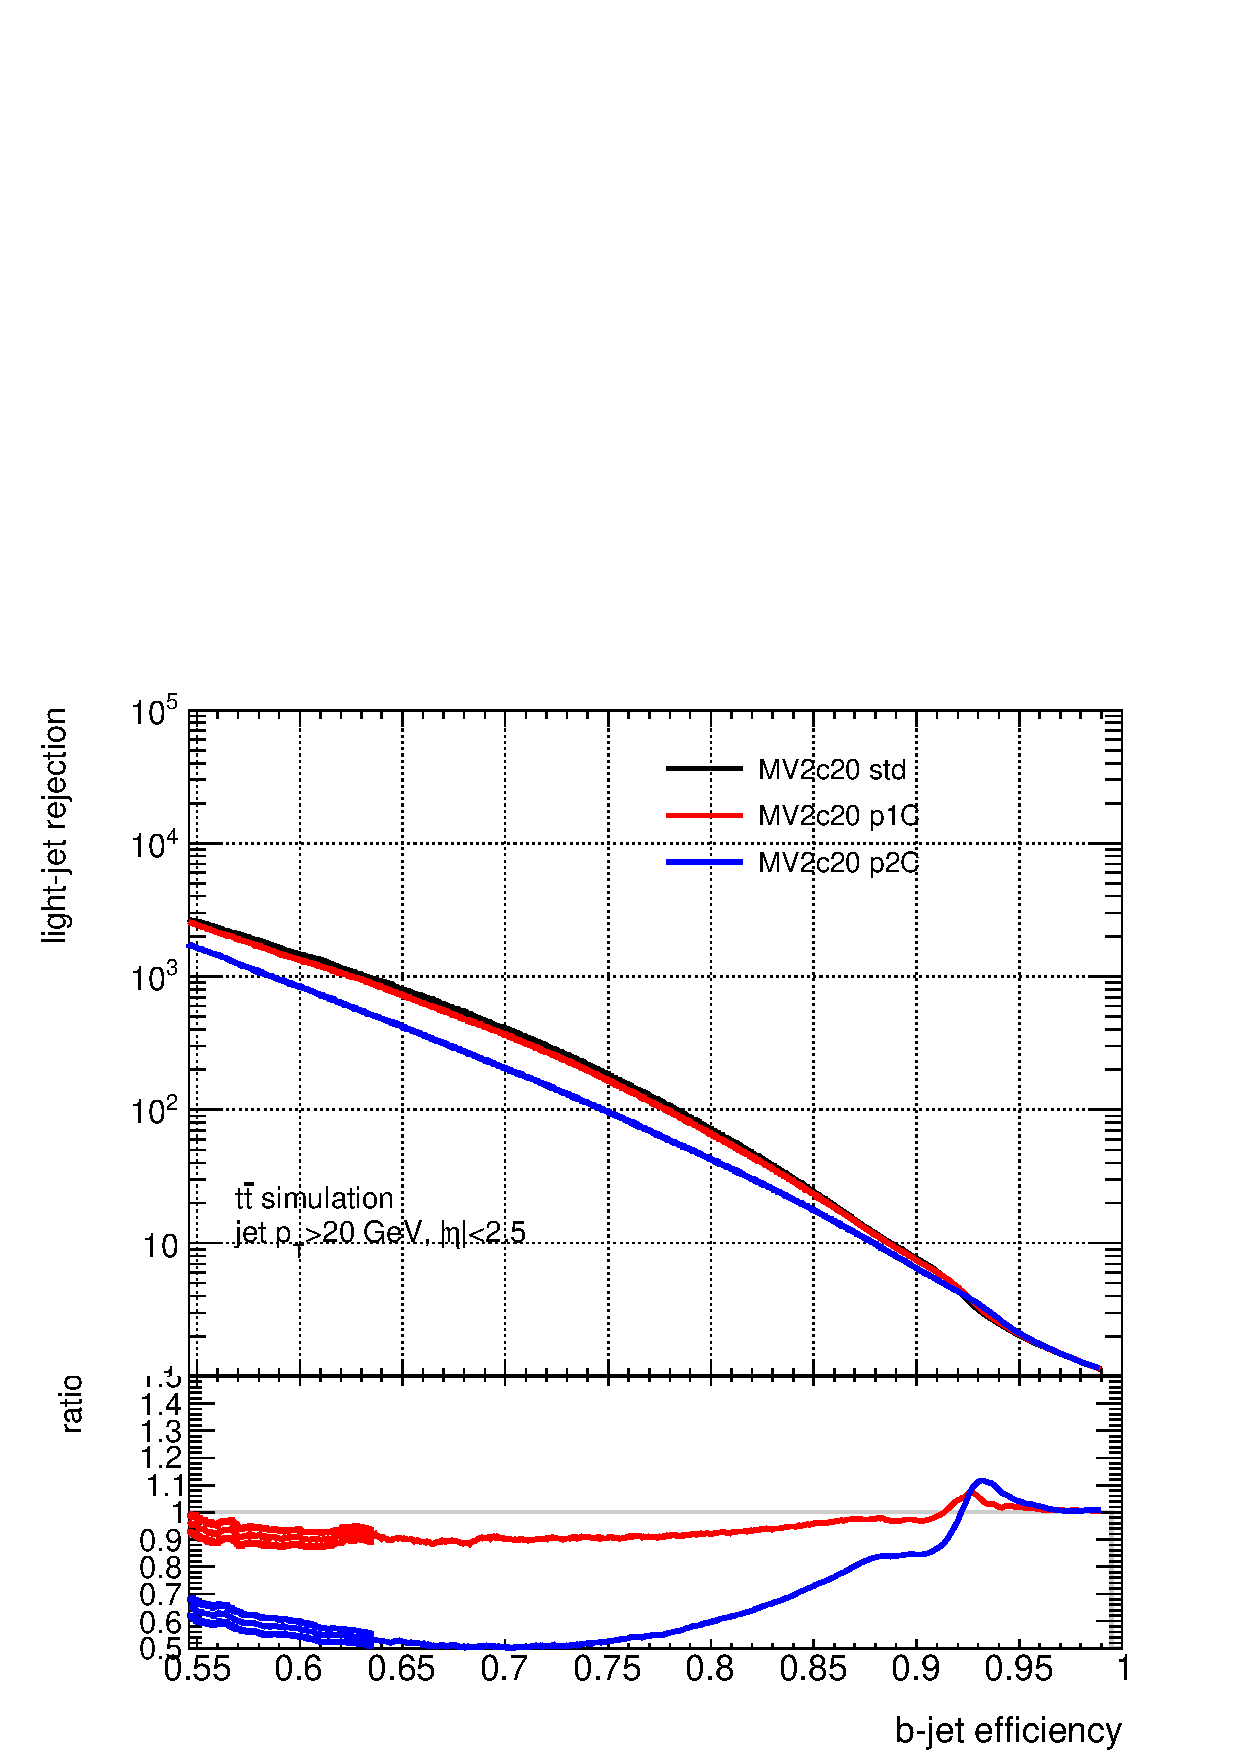
\includegraphics[width=0.45\textwidth]{Images/IBL_paper/chapter02_Physics/btagging/bVSlight__MV2c20.pdf}
\includegraphics[width=0.45\textwidth]{Images/IBL_paper/chapter02_Physics/btagging/bVSc__MV2c20.pdf}
\caption{\label{fig:btagging_inclusiveROCcurve} Performance of the $b$-tagging algorithm MV2c20 expressed in terms of light (on the left) or $c$-jet (on the right) rejection as a function of $b$-tagging efficiency, obtained by scanning the BDT discriminant. The algorithm is applied to jets from top pair events. The performance of the \runone and \runtwo detector layouts are compared, where the latter includes IBL. The rejection is defined as $R=1/\epsilon$, with $\epsilon$ being the tagging efficiency.}
\end{figure}

The input variables obtained from the three basic algorithms are then combined making use of a boosted decision tree algorithm to discriminate $b$-jets from either light ($u$,$d$,$s$-quark or gluon jets) or $c$-jets. Results in this sections are presented for the MV2c20 algorithm, for which the training is performed on a set of at least 5 million top pair events, using the $b$-jets as signal and a mixture of 80\% light-jets and 20\% $c$-jets as background. In order to perform a fair comparison, the algorithms have been re-trained separately for the ATLAS \runone geometry, without IBL, and the ATLAS \runtwo geometry, which includes the IBL.

The inclusive $b$-tagging performance on top pair events, after a very basic jet selection ($p_{T}>20$~GeV and $|\eta|$<2.5\%), is shown in Figure~\ref{fig:btagging_inclusiveROCcurve}. The additional of IBL improves the $b$-tagging performance in terms of light-jet rejection between a factor of 3 or 4 for $b$-jet tagging efficiencies up to 85\%.  The improvement in $c$-jet rejection is smaller and ranges approximately from 80\% to 20\% for $b$-jet tagging efficiencies from 50 to 75\%. Physics analyses will most often profit from the improved performance by re-tuning their $b$-tagging requirements in such a way to keep the background rejection the same but have an increased signal efficiency: this is shown in Table~\ref{tab:btagging_fixedRejection}. As an example, adding the IBL allows to keep the light-jet rejection rate at 100 while improving the $b$-jet tagging efficiency from 72\% to 79\%, with a relative improvement of 10\% on the $b$-tagging efficiency for each tagged jet in the event.

\begin{table}
\begin{center}
\begin{tabular}{lccc}
\hline
Light-jet rejection                                     & $b$-jet efficiency w/o IBL & $b$-jet efficiency with IBL \\ \hline
1000                                                            & 57\%     & 65\% \\
100                                                            & 71\%     & 79\% \\
10                                                            & 84\%     & 90\% \\ \hline
\hline
Constant $c$-jet rejection                                     & $b$-jet efficiency w/o IBL & $b$-jet efficiency with IBL \\ \hline
20                                                            & 56\%     & 62\% \\ 
10                                                            & 63\%     & 68\% \\ 
5                                                              & 72\%     & 76\% \\ \hline
\end{tabular}
\caption{\label{tab:btagging_fixedRejection} $B$-jet tagging performance expressed in terms of $b$-jet efficiency for a fixed light- or $c$-jet rejection, comparing the \runone and \runtwo detector layouts, where the latter includes IBL, and as derived from jets from top pair production, which pass the $p_{T}>20$~GeV and $|\eta|<2.5$ selection requirements.}
\end{center}
\end{table}

The $b$-tagging performance depends strongly on jet transverse momentum ($p_{T}$),
%and pseudo-rapidity ($\eta$), 
following the variation in underlying impact parameter resolution and tracking efficiency. The dependence of the performance on jet $p_{T}$ is shown in Figure~\ref{fig:btagging_vsPT}.
%, while the dependence on $\eta$ is shown in Figure~\ref{fig:btagging_vsETA}. 
The largest improvements are seen at low $p_{T}$, where the closeness of the IBL to the interaction region allows to reduce significantly the impact of multiple scattering. As an example, the improvement in light-jet rejection ranges from a factor of 3-4 up to $p_{T}=100$~GeV, a factor of 2 at $p_{T}=150$~GeV, leveling to only a very slight  improvement for jet $p_{T}$ above 250 GeV. At very high jet $p_{T}$ the tracking efficiency and resolutions are limited by shared clusters from collimated tracks produced in the core of high $p_{T}$ jets, a problem which becomes more severe with the insertion of IBL, which moves the radial distance of the closest pixel layer to the interaction region from $\approx 5$ to $\approx 3.3$~cm. The optimization of the tracking and pixel clustering algorithms to deal with such an environment~\cite{Aad:2014yva,ATL-PHYS-PUB-2015-006} has allowed to counteract such degradation effectively and keep the performance of the new \runtwo geometry at least at the same level of \runone even for very high $p_{T}$ jets. 

%{\bf Need to understand first bin in $p_{T}$ (especially for c-jets !!) and the last bins in $\eta$.}

\begin{figure}
\centering
\includegraphics[width=0.45\textwidth]{Images/IBL_paper/chapter02_Physics/btagging/jet_pt_MV2c20__l_flat}
\includegraphics[width=0.45\textwidth]{Images/IBL_paper/chapter02_Physics/btagging/jet_pt_MV2c20__c_flat}
\caption{\label{fig:btagging_vsPT} Performance of the $b$-tagging algorithm MV2c20 expressed in terms of light (on the left) or $c$-jet (on the right) rejection as a function of jet transverse momentum ($p_{T}$), while keeping the $b$-tagging efficiency fixed at 70\% in each $p_{T}$ bin. The performance of the \runone and \runtwo detector layouts are compared, where the latter includes IBL. The rejection is defined as $R=1/\epsilon$, with $\epsilon$ being the tagging efficiency.}
\end{figure}

%\begin{figure}[htb!]
%\centering
%\includegraphics[width=0.45\textwidth]{Images/IBL_paper/jet_eta_MV2c20__l_flat}
%\includegraphics[width=0.45\textwidth]{Images/IBL_paper/jet_eta_MV2c20__c_flat}
%\caption{\label{fig:btagging_vsETA} Performance of the $b$-tagging algorithm MV2c20 expressed in terms of light (on the left) or $c$-jet (on the right) rejection as a function of jet pseudo-rapidity ($\eta$), while keeping the $b$-tagging efficiency fixed at 70\% in each $\eta$ bin. The performance of the \runone and \runtwo detector layouts are compared, where the latter includes IBL. The rejection is defined as $R=1/\epsilon$, with $\epsilon$ being the tagging efficiency.}
%\end{figure}

The dependence on the average level of pile-up $\mu$ is presented in Figure~\ref{fig:btagging_vsMU}. While the overall performance is much improved with the addition of IBL, the dependence on pile-up in terms of relative degradation versus $\mu$ is almost unchanged, except in the case of the $c$-jet rejection, where a more severe degradation is seen with the IBL inserted. This study is performed on top pair events, where the distinction of the primary vertex from pile-up vertices is not a major concern.

\begin{figure}
\centering
\includegraphics[width=0.45\textwidth]{Images/IBL_paper/chapter02_Physics/btagging/avgmu_MV2c20__l_flat}
\includegraphics[width=0.45\textwidth]{Images/IBL_paper/chapter02_Physics/btagging/avgmu_MV2c20__c_flat}
\caption{\label{fig:btagging_vsMU} Performance of the $b$-tagging algorithm MV2c20 expressed in terms of light (on the left) or $c$-jet (on the right) rejection as a function of the average pile-up level $\mu$, while keeping the $b$-tagging efficiency fixed at 70\% in each $\mu$ bin. The performance of the \runone and \runtwo detector layouts are compared, where the latter includes IBL. The rejection is defined as $R=1/\epsilon$, with $\epsilon$ being the tagging efficiency.}
\end{figure}


%\begin{figure}
%  \begin{center}
%  \includegraphics[width=0.5\textwidth]{2d-cut.pdf}
%  \caption[JetFitterCharm 2-dimensional cut plane]{
%Two-dimensional distribution of the JetFitterCharm anti-$b$ ($\log(P_c/P_b)$) and anti-light ($\log(P_c/P_{\rm light})$) discriminants. The density of red, green, and blue reflect the density of $b$, $c$, and light jets, white areas are a mix of all three \flavours, whereas black areas lack any jets. The `medium' calibrated operating point selects jets above a certain threshold in both anti-$b$ and anti-light discriminants.
%Ridge structures arise from two features of the algorithm which concentrate values in the input space. The first feature is the use of discrete kinematic bin inputs, $\eta^{\rm cat}$ and $\pt^{\rm cat}$. The second is the substitution of default values when the ordinary input values would not be physically meaningful, for example when no secondary vertex is found. The resulting high density structures can be seen in the lower-center and upper-left region of the plot.}
%  \label{fig:2dcut}
%  \end{center}
%\end{figure}




%\begin{figure}
%  \begin{center}
%  \includegraphics[width=0.5\textwidth]{2d-cut.pdf}
%  \caption[JetFitterCharm 2-dimensional cut plane]{
%Two-dimensional distribution of the JetFitterCharm anti-$b$ ($\log(P_c/P_b)$) and anti-light ($\log(P_c/P_{\rm light})$) discriminants. The density of red, green, and blue reflect the density of $b$, $c$, and light jets, white areas are a mix of all three \flavours, whereas black areas lack any jets. The `medium' calibrated operating point selects jets above a certain threshold in both anti-$b$ and anti-light discriminants.
%Ridge structures arise from two features of the algorithm which concentrate values in the input space. The first feature is the use of discrete kinematic bin inputs, $\eta^{\rm cat}$ and $\pt^{\rm cat}$. The second is the substitution of default values when the ordinary input values would not be physically meaningful, for example when no secondary vertex is found. The resulting high density structures can be seen in the lower-center and upper-left region of the plot.}
%  \label{fig:2dcut}
%  \end{center}
%\end{figure}


%\begin{table}
%\begin{center}
%\begin{tabular}{c|c c | c c c }
%%% \multicolumn{6}{c}{$\charm$-tagging} \\ \hline
%Operating Point & $\log (P_\charm / P_\bottom$) & $\log (P_\charm / P_\light$) & $\epsilon_\charm$ & $1/\epsilon_\bottom$ & $1/\epsilon_\light$ \\ \hline
%Loose & $> -0.9$ & -- & 0.95 & 2.5 & 1.0 \\
%Medium & $> -0.9$ & $> 0.95$ & 0.20 & 8.0 & 200 \\
%\end{tabular}
%\caption[\ctagging operating points]{\ctagging operating points. Charm tagging requires two cuts: one to reject \bottom jets, and another to reject light jets. The approximate efficiency for \charm jets along with the rejection for \bottom and \light jets, with $\pt > 20\,\text{GeV}$ and $|\eta| < 2.5$ as estimated on $\ttbar$ events, are also given.}
%%GP Dan, are the efficiencies estimated on ttbar events?
%\label{tab:ops}
%\end{center}
%\end{table}

%GP temporary, just not to have the references on top




%The IBL upgrade was also combined to the replacement of the beam pipe, a l
\subsection{IBL Layout Overview}
% Chapter coordination:

%During the first long shutdown of the LHC machine, a new pixel layer was added between the Pixel B-layer and the beam pipe in the ATLAS detector.
The IBL is located at a nominal distance of \SI{33.5}{\milli\meter} from the beam axis, where this distance refers to the sensors position and it is the closest layer to the interaction point of the ATLAS Detector as shown in  Figure~\ref{fig:NewID}. Given the small sensor distance from the beam axis (compared with \SI{50.5}{\milli\meter} for the Pixel B-Layer), the sensors and front-end electronics must cope with a much higher hit rate and radiation with respect to the other layers.%and maximum radiation doses of respectively  \SI{5e15}{\nq} non ionizing energy loss (NIEL) and  \SI{250}{\mega\radian} total ionizing dose (TID) during \runone operation.
To address these requirements, a new front-end read-out chip has been developed, the FE-I4~\cite{fei4_manual} and two silicon sensor technologies were developed.\\
%The FE-I4 specifications satisfy the requirements of radiation tolerance and read out efficiency at high luminosity. In addition, the FE-I4 chip has a substantially larger active area compared with that of the existing FE-I3\footnote{The FE-I3 is the chip that is used for the other layers of the Pixel Detector} front-end pixel chip and  the pixel size has been reduced to $\SI{250}{} \times \SI{50}{\micro\meter\squared}$. 
\begin{table}
\centering
\begin{tabular}{lc}
\hline \hline
	 & Value\\
\hline
Number of staves & 14 \\
Number of physical modules per stave & 20  (12 Planar, 8 3D)\\
%Number of DCS modules per stave & 16 \\
Number of FEs per stave & 32 \\
Coverage in $\eta$, no vertex spread & $|\eta|\,<\,3.0$ \\
Coverage in $\eta$, 2$\sigma$ (\SI{122}{\milli\meter}) vertex spread & $|\eta|\,<\,2.58$ \\
Active $|z|$ stave length (\SI{}{\milli\meter}) & 330.15 \\
Geometrical acceptance in $z$ min, max (\%) & 97.4, 98.8 \\
Stave tilt in $\phi$ (degree) & 14 \\
Overlap in $\phi$ (degree) & 1.82 \\
Center of the sensor radius (\SI{}{\milli\meter}) & 33.5 \\
Radiation length at $z$ = 0  (\SI{}{\xzero}) & 1.9\\
\hline \hline
\end{tabular}	
\caption{Main layout parameters for the IBL detector. The quoted radiation length is averaged over the stave width and includes the IBL support and positioning tubes.
\label{tab:LayoutTable}}
\end{table}


%The sketch in Figure~\ref{fig:IBLView2} represents the IBL detector and its services. 

\begin{figure}
\begin{center}
 \includegraphics[width=0.61\textwidth, angle = -90 ]{Images/ibl_paper/chapter03_Overview/NewID.pdf}
\caption{The layout of the ATLAS tracking system with the additional layer of IBL. }
\label{fig:NewID}
\end{center}
\end{figure}


%\begin{figure}[!htb]
%\begin{center}
%\includegraphics[width=0.8\textwidth]{Images/ibl_paper/chapter02_Physics/Pixel_IBL_rendering.pdf}
%\caption{View of the IBL detector as positioned in the Pixel detector.}
%\label{fig:IBLView1}
%\end{center}
%\end{figure}

%\begin{figure}[!htb]
%\begin{center}
%\includegraphics[width=0.8\textwidth]{Images/ibl_paper/chapter02_Physics/IBL_rendering.pdf}
%\caption{Longitudinal view of the IBL detector and its services. 
%The insert shows an enlarged view of the detector with its modules arranged cylindrically around the beam pipe.}
%\label{fig:IBLView2}
%\end{center}
%\end{figure}

\begin{figure}
\begin{center}
 \includegraphics[width=0.8\textwidth]{Images/ibl_paper/chapter03_Overview/IBL_Layout.pdf}
\caption{ IBL layout: (a) Longitudinal layout of Planar and 3D modules on a stave. (b) An $r-\phi$
               section showing the beam pipe, the IPT, the staves of the IBL detector and the IST.
               (c) An exploded $r-\phi$ view of the corner of a 3D module fixed to the stave. }
\label{fig:IBLLayout}
\end{center}
\end{figure}
The most important layout parameters of the IBL detector are listed in Table~\ref{tab:LayoutTable} and a picture of the layout is shown in Figure~\ref{fig:IBLLayout}. The detector consists of 14 mechanical support (staves) equipped with pixel silicon modules surrounding the beam pipe, providing full azimuthal ($\phi$) coverage for high transverse momentum particles. %The nominal layer radius, i.e. the distance from the beam axis to the sensor center-of-mass, is \SI{33.5}{\milli\meter}.
Each stave hosts the electrical and cooling services to 20 pixel modules that are attached to the stave and provide a $|\eta|$ coverage up to 3. Two module types~\cite{IBL_mod_proto} are installed on each stave based on two different silicon sensor technologies: Planar and 3D. Planar sensors populate the central stave region, while 3D sensors the side region, as shown in Figure~\ref{fig:IBLLayout}. The forward region of the staves are populated by 3D sensors where they can guarantee a better z-resolution in the tracking reconstruction after heavy irradiation due to the electrode orientation. The details about the sensors are given in Section~\ref{sec:mod_sensor}. % A total of 12 Planar n-in-n sensors, similar to the present Pixel detector, each bump-bonded to  two FE-I4 readout chips, populate the central stave region. Four 3D sensors, for the first time in a particle physics tracking detector, each bump-bonded to one FE-I4 chip, populate each end of the stave. The staves  are mounted with the sensors facing the beam pipe. 
The staves are inclined by \SI{14}{\degree} with respect to the radial direction in order to achieve an overlap of the active area between staves. This tilt also compensates for the Lorentz angle of drifting charges in the case of Planar sensors, and the effect of partial column inefficiency for normal incidence tracks in the case of 3D sensors. Due to space constraints, the sensors are not shingled along the stave (in $z$). However to minimize the dead region, modules are glued on the stave with a physical gap of \SI{200}{\micro\meter}.\\
%In the End of Stave (EoS) region the detector services are connected to extensions that reach the Inner Detector End-Plate (PP1) where the connections to the external and fixed services are made after installation in ATLAS. At PP0 the cooling pipe of the stave is attached at each end to \SI{3}{\meter} length pipes. Also at PP0, the internal (Type 0) electrical services, providing data transmission and power to the modules, are connected to $\sim$\SI{3}{\meter} in length (Type I) electrical services.
A comparison between the IBL technical characteristics and the 3 layer Pixel Detector is reported in Table~\ref{tab:TableComparison}.

\begin{table}
	\centering
	\begin{tabular}{lcc}
	\hline \hline
	 & Pixel & IBL \\
	\hline
Active Surface (\SI{}{\meter\squared}) &  1.73 &  0.15 \\
Number of channels (x 10$^{6}$) & 80.36 & 12.04 \\
	\hline
	Pixel size (\SI{}{\micro\meter\squared}) & 50$\times$400 & 50$\times$250 \\
	Pixel array (FE-I4 chip) & 18$\times$160 & 80$\times$336 \\
	Chip size (\SI{}{\milli\meter\squared}) & 7.6$\times$10.8 & 20.2$\times$19.0 \\
	Active Fraction (\SI{}{\percent}) & 74 & 89 \\
	Analog current (\SI{}{\micro\ampere\per\pixel}) & 26 & 10 \\
	Digital current (\SI{}{\micro\ampere\per\pixel}) & 17 & 10 \\
	Analog voltage (\SI{}{\volt}) & 1.6 & 1.4 \\
	Digital voltage (\SI{}{\volt}) & 2.0 & 1.2 \\
	Data out transmission (\SI{}{\mega\bit\per\second}) & 40 & 160 \\
	\hline
Sensor type & Planar & Planar / 3D \\
Sensor thickness  (\SI{}{\micro\meter}) & 250 & 200 / 230 \\
Layer thickness  (\SI{}{\xzero})  & 2.8  & 1.9  \\
Cooling fluid & C$_3$ F$_8$ & CO$_2$  \\
\hline \hline
	\end{tabular}
	\caption{Comparison of the main characteristics of the Pixel detector and the IBL detector.}
	\label{tab:TableComparison}
\end{table}

The IBL volume, which contains  the staves and the services, is the space between an external Inner Support Tube (IST) fixed on the Pixel structure and a precision mechanical support called the Inner Positioning Tube (IPT). The central part of the ATLAS beam pipe is slid into the IPT tube and attached to it.
A key feature of this design approach is that independent volumes are generated and the fast removal of either the beam pipe with respect to the IBL package, or the IBL and beam pipe with respect to the Pixel package, are allowed. 
As the Pixel Detector was on the surface during 2014 for repair and service refurbishment, the IST was inserted there.
The IBL package, including the beam pipe, was then slid inside the IST once the Pixel detector was integrated and fully connected in the cavern.\\
The reduction of the material budget leads to an optimization of the tracking performance.
The averaged over $\phi$ IBL radiation length is 1.9 X$_0$ for normal incidence tracks  at $z = 0$ and it corresponds to $\sim$ \SI{70}{\percent}  of that for the Pixel B-Layer\footnote{The as-built IBL radiation length has been evaluated and then confirmed  in collisions data-taking. The difference with respect to the estimate reported in the IBL TDR~\cite{Capeans:1291633} is mainly due to a reduced initial estimate of the module material and the addition of the IPT.}. 
A lower radiation length has been achieved by using a new low-mass module design, a local support structures (staves) made of low density carbon foam, the use of CO$_2$ evaporative cooling that optimizes the mass flow and the pipe size and using aluminium conductors for the electrical power services. Table~\ref{tab:MaterialBudget} reports the main contributions to the IBL material budget. Figure~\ref{fig:IBLMaterialBudget} shows the
 material traversed by a track of origin $z = 0$ as a function of $\eta$, smeared over the 
 azimuthal angle.


\begin{table}
	\centering
	\begin{tabular}{lc}
	\hline \hline
	Item & Value (\SI{}{\xzero})\\
	\hline
	Beam pipe & 0.32 \\
	IPT & 0.12 \\
	Module &  0.76 \\
	Stave   &  0.6 \\
	Services   & 0.19  \\
%	Coolant  & ?? \\
	IST   &  0.21 \\
	\hline
	 IBL total   & 1.88 \\
	\hline \hline
	\end{tabular}
	\caption{Averaged IBL material budget over the azimuthal angle $\phi$ for normal incident tracks  at $z = 0$.  The beam pipe material is excluded from the IBL total. 
	\label{tab:MaterialBudget}}
\end{table}




\begin{figure}
	\centering
	\subfloat[\label{fig:xo_linear}]{\includegraphics[width=0.47\textwidth]{Images/ibl_paper/chapter03_Overview/IBL_BP_material.pdf}}
	\subfloat[\label{fig:xo_log}]{\includegraphics[width=0.47\textwidth]{Images/ibl_paper/chapter03_Overview/IBL_BP_material_zoomed.pdf}}
	\caption{(a) Radiation length as a function of $\eta$  for different components of the IBL detector as implemented in the ATLAS geometry model. Different components are shown:  the beam pipe,  the detector  (IBL staves, modules and IPT),  the services (cooling and cables) and  the structures (IST, stave rings, endblocks, sealing ring area). (b) A zoomed view of the central  $|\eta|$ distribution.}
\label{fig:IBLMaterialBudget}
\end{figure}






%\subsection{Design of IBL detector}
\subsection{Module Layout}
%\subsection{Modules}
%\label{sec:mod}

%The IBL pixel detector module is a complex entity consisting of the sensor, the FE-chip(s) and the module flex hybrid and built with many different assembly steps. Two different types of modules are used for the IBL: Double-chip (DC) modules with Planar sensors and single-chip (SC) modules with 3D sensors. In section~\ref{sec:mod_bumping}  the bump bonding process for the connection between chips and sensors is discussed. The module flex hybrid is introduced in section~\ref{sec:mod_flex} whereas the final module assembly is covered in section~\ref{sec:mod_assembly}. Details of the dressed modules are discussed in section~\ref{sec:dressed_modules} and and the results of the production QA of the dressed modules are presented in section~\ref{sec:module_qa}

The basic building block of the IBL is the module. Due to the two sensor concepts used, the IBL modules differ in size.
For Planar sensors the module consists of two FE-I4 chips connected to one sensor tile. For 3D sensors the module consist of one
FE-I4 chip connected to one sensor. A module consists of the following parts:

\begin{itemize}
\item the Planar or 3D sensor.
\item one or two FE-I4 chips each containing 26,880 pixel cells with amplifying circuitry.
\item a double-sided, flexible printed circuit (referred to as module flex).
\end{itemize}

The FE-I4 chip is described in section~\ref{sec:FEI4},  the two sensors concepts are treated in section~\ref{sec:mod_sensor} and the module flex is presented in section~\ref{sec:mod_flex}.

\subsubsection{The FE-I4 redout chip}
\label{sec:FEI4}
%The readout chip used in the first version of the Pixel detector is not capable of coping with the expected hit occupancies and radiation doses foreseen at the IBL radius, so a completely new readout chip architecture was designed.
\begin{figure}
\centering
{\includegraphics[width=0.5\textwidth]{Images/IBL_Paper/chapter04_Modules/FEI4.png}}
\caption{Picture of a FE-I4 chip and a to-scale picture of an FE-I3 chip. The pixel matrix and the approximately \SI{2}{\milli\meter} wide periphery can be seen.}
\label{fig:FEI4}


\end{figure}
\begin{figure}
\centering
\subfloat[Schematic view of the analog pixel cell]{\label{fig:FEI4_analog}\includegraphics[width=0.8\textwidth]{Images/IBL_Paper/chapter04_Modules/FEI4_Analog.png}}
\\
\subfloat[Block diagram of the digital 4-pixel region.]{\label{fig:FEI4_digi}\includegraphics[width=0.8\textwidth]{Images/IBL_Paper/chapter04_Modules/FEI4_Digital.png}}
\caption{Analog and digital logic of the FE-I4 chip.}
\label{fig:FEI4_circuit}
\end{figure}
The FE-I4 is designed in a \SI{130}{\nano\meter} IBM CMOS feature size technology using thin gate oxide transistors to increase the radiation hardness. The large chip ($\SI{20.2}{\milli\meter}\times\SI{18.8}{\milli\meter}$) has an active area holding 26880 pixel, allocated in 80 columns (\SI{50}{\micro\meter} pitch) and 336 rows (\SI{250}{\micro\meter} pitch), and an approximately \SI{2}{\milli\meter} wide periphery, as shown in figure~\ref{fig:FEI4}.\\
One of the main advantage of the FE-I4 chip with respect to the FE-I3 is the lower power consumption, as it is shown in Table~\ref{tab:TableComparison}. The design of the analog and of the digital circuitry was optimized with a power consumption per pixel of \SI{26}{\micro\watt}, while it is \SI{75}{\micro\watt} for the FE-I3.\\
The analog part is a two stage charge sensitive amplifier plus discriminator design as shown in Figure~\ref{fig:FEI4_circuit}(a). The basic working principle of the two is described in Chapter 2.\\
A two-stage amplifier configuration is used, the first stage (Preamp) is a cascode amplifier while the second stage (Amp2) is a folded cascode AC coupled to the Preamp. The two-stage choice allows to provide enough gain before the discriminator while permitting the optimization in the choice of the preamp feedback capacitor ($C_{f1}$).
The preamplifier (Preamp) and second stage amplifier (Amp2) are AC coupled, and the feedback current of both amplifiers can be adjusted. These adjustments are implemented globally ($V_{fb}$ and $V_{fb2}$), so that all pixels of the matrix are affected simultaneously. For the preamplifier feedback an additional current adjustment using the 4-bit FDAC allows the fine tuning of the Time Over Threshold (\tot) response for each pixel individually. The output of the Amp2 is compared to a threshold voltage ($V_{th}$) by the discriminator. The Threshold voltage can again be adjusted globally as well as individually for each pixel.\\
The discriminator is built with a two-input voltage comparator and a threshold voltage generator. Signal shaping is only done by the preamp with an adjustable return to the baseline, while the second stage provides only the voltage gain, given by the ratio $\frac{C_c}{C_{f2}}$. The return to the baseline and the discriminator threshold are individually adjustable in each pixel, with dedicated local and global pixel registers. Two selectable capacitors are provided for analog calibration injection.\\
Additionally, each pixel contains test hit injection circuitries. Analog test signals are injected using a voltage step defined by the calibration voltage ($V_{cal}$) and two test charge injection capacitances ($C_{inj1/2}$), which can be selected independently.% The $V_{cal}$ parameter depends on a Pulser DAC as follow:
%\begin{equation}
%V_{cal}[V] = a[V] + b[\frac{V}{DAC}] \times PulserDAC[DAC].
%\end{equation}
Digital test hits are injected to an OR element at the output of the discriminator. The output of the analog readout chain of each pixel can be disabled using an AND connected to the discriminator output and the enable bit (EN) on each pixel. %The output (HitOut) can be connected to the HitOR bus which is routed to each pixel of the matrix using a logical OR and a pull down transistor, and this is low in case of any discriminator being above threshold. The HitOR signal at the wire bond pad is active high due to the an additional inverter in the periphery of the chip. This signal is used for test purposes and enables the selectable self trigger operation of the chip. Thanks the bus $I_{leakMon}$ can be used to measure the current that is compensated by the leakage current compensation logic implemented in the feedback circuitry of the preamplifier.
The feedback current of the preamplifier can be adjusted in function of the leakage current coming from the sensor, in order to compensate the latter after the irradiation.\\
Four pixels share a common digital logic cell for further hit processing as shown in figure~\ref{fig:FEI4_circuit}(b). The FE-I4 digital hit processing is based on the 4-pixel digital region. Detailed studies show that the transfer of the hit information to the chip periphery is the main inefficiency source at the expected IBL hit occupancy \cite{Malte_41}. The FE-I4 hit processing architecture therefore stores the hits in the pixel array close to the analog readout chain and the hits are processed only if a trigger signal is received. Detailed information on this architecture can be found in \cite{man_fei4b}. Four pixels share a set of five latency counters, while each pixel holds his own set of five \tot counters. A hit in one of the analog pixel cells allocates and starts the first unallocated latency counter to count down from the programmed latency (in units of \SI{25}{\nano\second}). The charge information belonging to this specific time stamp is stored in the buffers for all pixels connected to the 4-pixel digital region. An incoming Level-1 trigger in coincidence with the latency value of zero initiates the transfer of the hit data to the end of chip logic, and deallocates the latency counters and buffers. If no corresponding Level-1 trigger arrives, the hit information is deleted and the counter and buffers are deallocated as well.\\
Each of the readout chips holds two on-chip LDO (Low Drop Out) regulators (\cite{Malte_44} and \cite{Malte_45}) to generate the analog and digital supply voltages. These are linear regulators, which keep a constant output voltage independently of the input voltage and the load current. A minimum difference between the input voltage and the output voltage (dropout voltage) is used to achieve a high power efficiency. The on-chip LDOs are operated in partial shunt mode. This means that they are operated as usual LDO as long as the current consumption is above an adjustable minimum input current. If below, an additional current is shunted to ground by the regulators. This operation mode does not increase the power consumption of the FE-I4 chip as long as its current consumption in working conditions is above the shunt current. The advantage of this mode is the reduction of the transients in comparison to the pure LDO mode in case of load current fluctuations. This will happen in case of configuration of the FE-I4 or accidental configuration loss. The reference voltages needed for the operation of the two LDOs are generated on-chip.

\subsubsection{Sensors}
\label{sec:mod_sensor}

% added by sebastian

\begin{figure}
\subfloat[\label{fig:planar_collection}]{\includegraphics[width=0.48\textwidth]{Images/IBL_paper/chapter04_Modules/planar_principle.png}}
\subfloat[\label{fig:3d_collection}]{\includegraphics[width=0.48\textwidth]{Images/IBL_paper/chapter04_Modules/3d_principle.png}}
\caption{Charge collection mechanism in Planar (a) and 3D sensors (b)}
\end{figure}
Two sensor technologies are used in the IBL detector: the first is a improved version of the one used in the other layer of Pixel Detector, the Planar\cite{Planar} architecture, and a novel technology, the 3D\cite{3d} technology.
In the Planar technology the electrode are obtained on the surfaces of the bulk, the equipotential line are then parallel to the surface of the device. When the sensor is biased and a charge particle cross it, the holes and the electrons created by ionization drift towards the electrodes, moving across the bulk width as shown in Figure~\ref{fig:planar_collection}.\\
\begin{figure}[h]
	\centering
	 (a)~\includegraphics[width=0.95\textwidth]{./Images/ibl_paper/chapter04_Modules/Planar-edge-apix.png}\\
 	 (b)~\includegraphics[width=0.95\textwidth]{./Images/ibl_paper/chapter04_Modules/Planar-edge-ibl.png}\\
  \caption{Comparison of the edge designs of the (a) ATLAS pixel sensor and (b) Planar IBL pixel sensor. The inactive edge has been reduced from \SI{1100}{\micro\meter} to \SI{200}{\micro\meter}. In the guard-ring area cooler colours (such as blues) represent the n-implantation on the front-side of the sensor, warmer colours (such as reds) the p-implantation on the back-side. Figure is taken from Reference \cite{WittigPhd} with modifications.}
	 \label{fig:Planar-figure-edge}
\end{figure}
The design of the Planar sensor derives from the design of the sensor of the ATLAS Pixel Detector, which employs an n$^+$-in-n technology, where the n-side segmentation matches in size the front-end read-out electronics connected via bump-bonds. A guard-ring structure is placed on the p-side. To be compatible to the newly developed FE-I4 chip, the pixel dimensions have been shrunk to \SI{250}{} $\times$ \SI{50}{\square\micro\meter}.\\
A key features of the IBL Planar sensors is the slim-edge design which enlarges edge pixels opposite to the guard-rings and it is possible for n$^+$-in-n sensors thanks to the double sided process. This design decision was based on an extensive study which analyzed the efficiency of the sensor in the guard ring area \cite{Planar-slim-edge-2012}. No changes in the breakdown behavior have been observed as the voltage drops take place on the p-side.  The number of guard-rings was optimized based on a complementary study, which evaluated the breakdown behavior after partial guard-ring removal \cite{Planar-guard-ring-removal-2010}.  Compared to the original ATLAS pixel sensor the number of guard-rings has been reduced from 16 to 13.  Also the cutting edge has been shifted nearer to the guard-rings. In Figure \ref{fig:Planar-figure-edge} the improvement of the slim-edge design for the IBL sensor in comparison to the edge design of the ATLAS pixel sensor is shown. The combination of all three modifications, moving the cutting edge as safety margin, reducing the number of guard-rings and extending the edge pixels beneath the guard-rings, allows the reduction of the inactive edge from \SI{1100}{\micro\meter} for the ATLAS pixel design to approximately \SI{200}{\micro\meter} for the slim-edge IBL design~\cite{WittigPhd}.
The substrate material is float zone enriched with oxygen with a <111> bulk crystal orientation and a resistivity of \SIrange{2}{5}{\kilo\ohm\centi\meter}.
The production of Planar sensor for the IBL was done at CiS\footnote{CiS: Forschungsinstitut f\"ur Mikrosensorik GmbH, Erfurt, Germany}. All details of the sensor design can be found in~\cite{WittigPhd}.\\
The pixels of the two central columns of the double-chip sensor are extended to \SI{450}{\micro\meter} to keeps a necessary gap between the two adjacent front-end chips. The pixels at the outer edges of the sensor tile are enlarged to \SI{500}{\micro\meter} length. The nominal outer dimensions of the sensor layout are \SI{41300}{\micro\meter} $\times$ \SI{18600}{\micro\meter}.
The positions of high-voltage contact pads on the p-side matches the flex design openings to allow wire bonding to the sensor. Fiducial marks on the p-side of the sensor allow proper alignment of the modules during stave loading. Those marks are placed outside the guard-ring area within the dicing streets in the inactive area of the sensor.
Metallize scratch patterns are placed on the p-side of the IBL sensor close to the dicing street. In combination with the four identifying sensor numbers implemented in the metal mask on the n- and p-side of the sensor, this allows a unique identification of the sensor throughout the whole quality assurance, assembly and mounting processing of IBL sensors and modules. Some further details of the sensor design can be found in~\cite{WittigPhd}.\\
In the 3D technology the electrodes penetrate the bulk in depth perpendicularly to the sensor surface. The electrode shape is columnar and the depletion region grows around the columns. In this configuration the holes and electrons drift parallel to the sensors surface. The drift distance is not related to the width of the device, but only to the pitch between electrodes of different type. Since the inter-electrodes pitch is of the order of \SI{50}{\micro\meter}, the average distance that the electrons and holes travel in the silicon bulk is reduced in 3D sensors with respect to Planar. The possibility of recombination after irradiation is then reduced. Given the 3D electrodes geometry, the full depletion is reached for lower voltage than the Planar technology and this reflects in a lower power consumption. Given those characteristics the 3D geometry is a very good candidate for high radiation environment, being less demanding in terms of cooling and bias voltage. The fabrication process of 3D sensors is more complex and the production yield is lower than the Planar. 3D sensors do not need to compensare the Lorentz effect, due to the orientation of the electric field which is parallel to the magnetic field in ATLAS.
Test-beam investigations have shown that even if the overall efficiency was showing the same performance of the Planar, the region of the column was slightly inefficient. \\
\begin{figure}
\centering
\includegraphics[width=\textwidth]{Images/ibl_paper/chapter04_Modules/3d_design.png}
\caption{\textbf{}Design of the columns of the FBK (left) and CNM (right) 3D sensors. This sketch is for illustration only and is not to scale.}
\label{fig:3d_design}
\end{figure}
In 3D pixel sensors, the column-like electrodes penetrate the substrate, instead of being implanted on the wafer surface. Thus, the depletion region grows coaxially to the columns. The $\approx\!$\SI{10}{\micro\meter} diameter columns are alternately n- and p-type doped defining the pixel configuration. The electrode spacing can be five to ten times smaller than the detector thickness (typically a few hundred microns), thereby dramatically reducing the charge-collection distance and depletion voltage. 
%The Planar technology is based on the successful design used in the Run~1 pixel detector, with several improvements. Most notably the inactive edges have been substantially reduced. The 3D sensor design~\cite{original_3d_paper} relies on column-like electrodes that penetrate the substrate, reducing the drift path with respect to the Planar approach while keeping a similar thickness and thus signal size.
%Planar sensor modules with two read-out chips cover the central region of the detector, \SI{75}{\percent} of the active area, while the forward $\eta$ regions are populated with single-chip 3D sensor modules. 
Both sensor types showed satisfactory performance in terms of noise, hit reconstruction efficiency and uniformity before and after irradiations to the fluence level of \SI{5e15}{n$_{eq}$\per\square{\centi\meter}} NIEL, as required for the operation inside the IBL~\cite{IBL_mod_proto}. 3D sensors showed an advantage in terms of power consumption due to the lower operational voltage whereas the Planar sensors proved their excellent performance during the Run~1 operation of the ATLAS pixel detector.\\ %In section~\ref{sec:Planar_design} and section~\ref{sec_3d_design} the Planar resp. 3D sensor design for the IBL is presented before in section~\ref{sec:sensor_qa} the results of the quality assurance during the sensor productions are discussed. Further performance results of both sensor types including test beam measurements are presented in detail in~\cite{IBL_mod_proto}.  
The 3D sensors for IBL have been fabricated at FBK\footnote{FBK: Fondazione Bruno Kessler, Trento, Italy} and CNM\footnote{CNM: Centro Nacional Micro-electronica, Valencia, Spain}~\cite{ds-cnm,ds-fbk}. Starting wafers were Float Zone, p-type, with \SI{100}{\milli\meter} diameter, $<100>$ crystal orientation, \SI{230}{\micro\meter} thickness, and a very high resistivity (10 to \SI{30}{\kilo\ohm\centi\meter}). Columnar electrodes, \SI{12}{\micro\meter} wide, were obtained by Deep Reactive Ion Etching (DRIE) and dopant diffusion from both wafer sides (n+ columns from the front side, p+ columns from the back side), without the presence of a support wafer. By doing so, the substrate bias can be applied from the back side, as in Planar devices. Figure~\ref{fig:3d_design} shows details of the 3D column layout.
The sensor design is detailed in~\cite{DAVIA_NIMA694_2012} and also reported in~\cite{IBL_mod_proto}. Each of the 80 $\times$ 336 pixels has a size of \SI{250}{\micro\meter} $\times$ \SI{50}{\micro\meter}, and contains two read-out (n$^+$) columns (two-electrode configuration), with an inter-electrode spacing between n$^+$ and p$^+$ columns of $\approx$\SI{67}{\micro\meter}. For yield reasons, it was decided to have single-sensor tiles (8 per wafer). A \SI{200}{\micro\meter} wide region separates the active pixel area from the physical edge of the tile. The nominal dimension of the 3D sensors are \SI{20400}{\micro\meter} $\times$ \SI{18700}{\micro\meter} (without scribe-lines).
The main differences between FBK and CNM productions are the following:
\begin{itemize}
\item FBK sensors have traversing columnar electrodes, i.e., \SI{230}{\micro\meter} deep; on the contrary, for CNM sensors, electrode etching is stopped $\approx$\SI{20}{\micro\meter} before reaching the opposite surface;
\item FBK sensors have surface isolation between n+ electrodes is obtained by a p-spray layer on both wafer sides, whereas in CNM sensors, p-stops are used on the front side only;
\item FBK sensors have the edge isolation based on a multiple ohmic column fence able to stop the lateral spread of the depletion region, whereas in CNM sensors a 3D guard-ring, surrounded by a double row of ohmic columns, is used to sink the edge leakage current.
\end{itemize}
More details on FBK and CNM 3D technologies used for the IBL production can be found in~\cite{GIACOMINI_TNS_13} and~\cite{PELLEGRINI_NIMA_13}, respectively. Table~\ref{tab:sensors} summarises the main parameters of  the IBL sensors. 



\begin{table}
\centering
\begin{tabular}{p{6cm}ccc}
\hline \hline
  % after \\: \hline or \cline{col1-col2} \cline{col3-col4} ...
\textbf{Parameter} & \textbf{Planar} & \textbf{3D CNM} & \textbf{3D FBK} \\ \hline \hline
Tile dimension [\SI{}{\micro\meter\squared}]    & 41315 $\times$ 18585 % 41315 x 18585 (nominal: 41300 x 18600)
                                                & 20450 $\times$ 18745 % 20450 x 18745 (nominal: 20400 x 18700) 
                                                & 20450 $\times$ 18745 \\
Sensor thickness [\SI{}{\micro\meter}]  & 200 & 230 & 230  \\
Pixel size (normal) [\SI{}{\micro\meter\squared}] 
                                                & 250 $\times$ 50 & 250 $\times$ 50 & 250 $\times$ 50 \\
Pixel size (tile edge) [\SI{}{\micro\meter\squared}]
						& 500 $\times$ 50 & 250 $\times$ 50 & 250 $\times$ 50 \\ 
Pixel size (tile middle) [\SI{}{\micro\meter\squared}]
						& 450 $\times$ 50 & - & - \\ 
Edge isolation       & Guard-rings & 3D guard-ring, fences & Fences \\
%Extension of efficiency for external rows [Dy @ 50% efficiency]						
Pixel isolation      & p-spray     & p-stop on n-side &	p-spray \\ \hline 
%Column depth         &             &  \SI{200}{\micro\meter}  &  \SI{230}{\micro\meter}  \\ 
%Column diameter      &             & \SI{12}{\micro\meter}  &  \SI{12}{\micro\meter}  \\						
Operating bias voltage unirradiated / \SI{5e15}{\nq}  [\SI{}{\volt}]
                                   & 80 / 1000 & 20 / 160  & 20 / 160 \\ 
 Operational power at \SI{-15}{\celsius} and after \SI{5e15}{\nq} [\SI{}{\milli\watt\per\centi\meter\squared}] 
                     &    90   
                     &    15                
                     &    15  \\ 
 \hline \hline					 
\end{tabular}
\caption{Summary of the main design specifications of Planar and 3D sensors.}
\label{tab:sensors}
\end{table}


\subsubsection{Module Flex Hybrid}
\label{sec:mod_flex}

The module flex hybrid is a double-sided, flexible printed circuit board which routes the signal and power lines between the stave flex (described later in this chapter) and the FE-chips and provides the bias voltage for the sensor via copper traces. Since both types of modules are on each stave, single-chip 3D modules and double-chip Planar modules, two types of module flexes are needed. From the layout and schematic point of view the DC module flex is a pair of two SC module flexes. The envelope of the module flex is defined by the sensor dimensions and it is slightly narrower than the sensor width. In Figure~\ref{fig:module_flexes} a picture of single-chip and double-chip module flex hybrid is shown.

\begin{figure}
\centering
\includegraphics[width=0.4\textwidth, angle=270]{Images/ibl_paper/chapter04_Modules/module_flexes.pdf}
\caption{Photographs of a double-chip (left) and a single-chip module flex hybrid (right). The frame and flex extension allows testing of the module before loading on stave. It is cut during the stave loading procedure at a cutting line indictated as white line slightly outside the bare module envelope.}
\label{fig:module_flexes}
\end{figure}

The module flexes are glued to the sensors's backside and are connected to the longitudinal stave flex which is located at the backside of the stave via thin transversal wings, one per read-out chip. The layer stack is \SI{130}{\micro\meter} consisting of two copper layers, each \SI{18}{\micro\meter} thick, and the dielectric kapton layers, which are all glued together with acrylic adhesive layers. Passive components are mounted on the module-flex for decoupling and filtering of the read-out chips and for terminations of the signal traces. The module temperature is remotely monitored via a Negative Temperature Coefficient (NTC) thermistor added on the module-flex. All passive components are soldered on the top layer of the flex. Special emphasis is given to high voltage (HV) routing and filtering since the flex hybrid has to be functional up to \SI{1000}{\volt}. To avoid HV discharges, sufficient space between HV traces and signal and low voltage (LV) traces are introduced. The HV capacitor is encapsulated with a polyurethane resin and \SI{27}{\micro\meter} thick kapton cover layers are used on the top and bottom of the flex.

All signal and power traces of the module flex are routed to a 50-pin connector outside the module area used during production testing of the modules. Underneath the connector a stiffener is added to make the frame more rigid. Both module flex hybrid types use the same connector, and an intermediate wire bond connection is necessary to connect all signal and power lines from the flex to the connector on the frame. Prior to the loading of the module to the staves this connector area is cut away. The cutting line is about \SI{1.5}{\milli\meter} away from the sensor. The cutting area of the module flex hybrid is smaller in width than the stave flex hybrid wings to avoid any part of the residual cut area touching other components of the detector. Finally the wire bond pads for the intermediate connection are re-used to connect the modules flex hybrid to the stave flex hybrid wings using wedge bonding. 

The module flex hybrids were produced at Phoenix\footnote{Phoenix S.r.l., Via Burolo 22, 10015 Ivrea (Torino), Italy} and surface mounted device (SMD) component loading, including encapsulation, was performed at Mipot\footnote{Mipot S.p.A., Via Corona 5, 34071 Cormona, Italy}. Basic quality assurance (QA) like testing of line integrity for open and shorted connections were done by the vendors and was followed by more detailed QA tests at the two module assembly sites. These QA procedures include HV standoff tests at 1.5~kV, visual inspection and dedicated cleaning to allow for high-quality wire bonding.


\subsubsection{Dressed modules}
\label{sec:dressed_modules}
\begin{figure}
	\centering

		\subfloat[\label{fig:SC_picture}]{		 \includegraphics[width=0.335\textwidth,angle=180]{Images/ibl_paper/chapter04_Modules/IBL_module_photo_SC_HD.jpg}}
		\subfloat[\label{fig:DC_picture}]{ \includegraphics[width=0.655\textwidth,angle=180]{Images/ibl_paper/chapter04_Modules/IBL_module_photo_DC_HD.jpg}}
  \caption{Photographs of a dressed IBL single chip module (a) and a double chip module (b). The flex extension visible on the top allows testing of the module before loading on stave. It is cut during the stave loading procedure at a cutting line slightly above the bare module.}
	\label{fig:module_pictures}
\end{figure}
In Figure~\ref{fig:module_pictures} pictures of a fully dressed single chip and a double chip module are shown. The modules are cut out of the handling frame.
The entire design of the module is optimized for low material budget wherever possible. The FE chips are thinned to \SI{150}{\micro\meter} and the sensor thickness is reduced to \SI{200}{\micro\meter} for Planar sensors and \SI{230}{\micro\meter} for 3D sensors. The thickness of the double sided flex has been chosen to be only \SI{130}{\micro\meter} and the number of SMD components is reduced to a minimum. Table~\ref{tab:module_x0} summarizes the thickness of the IBL modules and its parts in units of the radiation length X$_0$ for perpendicular particle penetration. The contributions of the different materials are averaged over the module size. The total thickness of a Planar IBL module is \SI{0.58}{\xzero} and \SI{0.61}{\xzero} for a 3D module. 
\begin{table}
\centering
\begin{tabular}{lc}
\hline \hline
	 & \SI{}{\xzero}\\
\hline
FE chip & 0.21 \\
Planar sensor & 0.24 \\
3D sensor & 0.27 \\
Module flex incl. SMD components & 0.13 \\
\hline
Sum for Planar module & 0.58\\
Sum for 3D module &  0.61\\
\hline \hline
\end{tabular}	
\caption{Breakdown of material budget for the IBL modules in thickness in units of the radiation length.}
\label{tab:module_x0}
\end{table}


\subsection{Stave Layout}
 % Chapter coordination: Claudia, Eric

The IBL modules are supported and cooled by means of fourteen mechanical supports, the staves, cylindrically arranged around the beam-pipe. In this section a description of the support stave and of the flexible printed circuits used as services for the stave is given.


\subsubsection{The support stave}

The support stave design is motivated by several important requirements:
\begin{itemize}
\item A low radiation length to improve physics performance,
\item An excellent thermal performances to cool down silicon sensors to maximize signal to noise and to prevent thermal runaway,
\item Good mechanical stability for the most efficient tracking performances,
\item A low thermal expansion coefficient of materials to reduce stress and increase stability.
\end{itemize}

%\paragraph{Design}
As shown in Figures~\ref{fig:StaveConcept}, \ref{fig:StaveCrossSection} the stave is an assembly of four main components: the cooling pipe, the carbon foam to drain the heat flux; carbon laminates to reinforce the stave stiffness (the face plate where module will be loaded and the back stiffener on the opposite side); and the peek to assemble the stave on fixations parts around the beam-pipe. These complex materials require specific manufacturing techniques. For example: carbon laminate requires fabrication in high pressure oven to obtain the required transverse thermal conductivity; assembly process require accurate gluing for material minimization; and the titanium cooling pipes require accurate machining and minimal wall thickness (\SI{0.12}{\milli\meter} wall thickness) compatible with high pressure  CO$_2$ operation. 

\begin{figure}
\begin{center}
% \includegraphics[width=0.8\textwidth]{Images/IBL_Paper/chapter05_Staves/StaveConcept.jpg}
 \includegraphics[width=0.8\textwidth]{Images/IBL_Paper/chapter05_Staves/BareStaveStructure_text.pdf}
\caption{Sketch of the support stave structure.}
\label{fig:StaveConcept}
\end{center}
\end{figure}

\begin{figure}
\begin{center}
 \includegraphics[width=0.8\textwidth]{Images/IBL_Paper/chapter05_Staves/Stave_section_WBG.pdf}
\caption{Stave section picture.}
\label{fig:StaveCrossSection}
\end{center}
\end{figure}

Minimizing materials is one of the most important requirements for the IBL detector to guarantee the required physics performances. For the support stave, this has led to a very aggressive design and choice of materials while maintaining a high level of reliability. The total material budget of the support stave structure is \SI{0.62}{\xzero} and the contribution of each part is  detailed in Table~\ref{tab:staveX0}. %The main properties of the used material in the support stave assembly are summarized in Table~\ref{tab:stavecomponents}.


\begin{table}
\centering
\begin{tabular}{l c c c c c }
\hline \hline
        Component & Material  & Volume/stave      & Eq. Thickness & X$_0$ & X/X$_0$  \\
                      &   &  (\SI{}{\centi\meter^3}) &             (\SI{}{\centi\meter})      & (\SI{}{\centi\meter})             & (\SI{}{\percent})      \\
\hline
% By Eric was
%Omega               &  K13C/RS3 & 2.02 & 0.144 & 21. 1 & 0.068 \\
%Glue layers & Stycast 2850FT & 3.29 & 0.234 & 8.97  &  0.2608\\
%Foam                             & K9 & 21.60 & 1.536 & 213 &   0.0721\\
%Ti pipe & Titanium T40           & 0.411 & 0.029 & 3.56 &  0.0821\\
%Face plate       &  K13C/RS3 & 1.903 & 0.135 & 21.1 & 0.0641 \\
%End of Stave fixation & Peek CA 40 & 2.51   & 0.178 & 25 &  0.0714\\
%Central fixation          & Peek CA 40 & 0.075 & 0.005 & 25 & 0.0021 \\

Back stiffener    &  K13C/RS3 & 2.02 & 0.144 & 21. 1 & 0.068 \\
Glue layers & Stycast 2850FT & 3.29 & 0.234 & 8.97  &  0.261\\
Foam                             & K9 & 21.60 & 1.536 & 213 &   0.072\\
Cooling pipe & Titanium T40           & 0.411 & 0.029 & 3.56 &  0.082\\
Face plate       &  K13C/RS3 & 1.903 & 0.0135 & 21.1 & 0.064 \\
End of Stave fixation & Peek CA 40 & 2.51   & 0.178 & 25 &  0.071\\
Central fixation          & Peek CA 40 & 0.075 & 0.005 & 25 & 0.002 \\
\hline
Total:              &  &  &  &  & 0.621 \\
\hline \hline
\end{tabular}   
\caption{Support stave radiation length budget.  %\textit{\bf Check digits!}
\label{tab:staveX0}}
\end{table}


%\begin{table}
%\centering
%\begin{tabular}{l c c c c c c }
%\hline \hline
%        Component & Density  & K      & CTE@\SI{20}{\celsius} & Young Mod. & Tensil  & Compressive  \\
%                     &  (\SI{}{\gram\centi\meter\squared})    & (\SI{}{\watt\per\milli\kelvin}) &       (\SI{}{\micro\meter\per\milli\celsius})            & (\SI{}{\giga\pascal})             & Strength (\SI{}{\mega\pascal})                & Strength  (\SI{}{\mega\pascal}) \\
%                      &  (\SI{}{\gram\centi\meter^3})    & (\SI{}{\watt\per\milli\kelvin}) &       (\SI{}{\micro\meter\per\milli\celsius})            & (\SI{}{\giga\pascal})             & Strength  & Strength  \\
%                      &     &  &                  &          & (\SI{}{\mega\pascal})                &  (\SI{}{\mega\pascal}) \\
%\hline
%%by Eric 
%%Grade 2 Titanium                        & 4.51 & 16.4 & 8.6 &102 & 430 & 340 \\
%%130 ppi K9 Carbon Foam  & 0.20 & 28.3 & $<1$ & 0.293 & 3.6 & 1.8 \\
%%RS3-K13C2U  &  & & &  & & \\
%% unirirectional prepreg  & 1.73 & (\emph{x/y}) 96 & (\emph{x}) -0.7 & (\emph{x}) 410 & & \\
%%0/90/0 layup  & & (\emph{z}) 5 & (\emph{y/z}) 15  &  (\emph{y/z}) 5.6 & & \\
%Titanium T40                        & 4.51 & 16.4 & 8.6 &102 & 430 & 340 \\
%K9 Carbon Foam  & 0.20 & 28.3 & $<1$ & 0.293 & 3.6 & 1.8 \\
%K13C2/RS3 &  & & &  & & \\
% unidirectional prepreg  & 1.73 & (\emph{x/y}) 96 & (\emph{x}) -0.7 & (\emph{x}) 410 & & \\
%K13C2/RS3 &  & & &  & & \\
%0/90/0 layup  & & (\emph{z}) 5 & (\emph{y/z}) 15  &  (\emph{y/z}) 5.6 & & \\
%
%\hline \hline
%\end{tabular}   
%\caption{Support stave materials main properties.
%\label{tab:stavecomponents}}
%\end{table}

%\subsubsection{Cooling performance}
An important design element of the stave is to remove the dissipated heat from the sensors and the read-out electronics. The target temperature of IBL sensor during operation is below \SI{-15}{\celsius}  in order to minimize the effects of the reverse annealing and the thermal runaway. An additional constrain and over-constraining requirement due to the beam pipe proximity is to cool down safely the modules during the beam-pipe bake-out phase that is meant to de-gas the beam pipe before the beams routinely circulation.
The CO$_2$ cooling liquid is chosen to achieve the required low temperature module operation while minimizing the pipe diameter and the associated radiation length. Because of the high CO$_2$ critical pressure (\SI{73.8}{\bar}(a) at \SI{31}{\celsius}), the thin wall titanium tubes must fulfill stringent pressure requirements.
Several simulations were performed to estimate the ultimate stave thermal performance (called Thermal Figure of Merit, $TFoM$), i.e. the thermal resistance between the cooling fluid and the sensor surface. In IBL detector conditions, the thermal runaway can be expressed as follow:

\begin{equation}
T_{sensor} = T_{coolant} + \frac{TFoM}{A_{sensor}} \times  (P_{chip} + P_{flex} + P_{sensor} )
\end{equation}
where $TFoM$ is the stave thermal figure of merit; $P_{chip}$ the chip dissipated power; $P_{flex}$ the dissipated power in the module flex; $P_{sensor}$ the dissipated power in the sensor calculated in worth case conditions; $A_{sensor}$ the  active sensor area.
In such condition the thermal runaway can be determined and was estimated to occur for the $TFoM > \SI{30}{\celsius\centi\meter^2\per\watt}$, as shown in Figure~\ref{fig:ThermalRunAway}.

\begin{figure}
\begin{center}
 \includegraphics[width=0.6\textwidth]{Images/IBL_Paper/chapter05_Staves/ThermalRunAway.pdf}
\caption{Sensor maximum temperature  with respect to the stave thermal figure of merit $TFoM$ at \SI{-40}{\celsius} evaporative cooling temperature.}
\label{fig:ThermalRunAway}
\end{center}
\end{figure}

A validation of the simulation is  illustrated in the  graph reported in Figure~\ref{fig:Temperature}a that shows the thermal results obtained on a stave prototype during the final design qualification. The $TFoM$ measured is  \SI{14}{\celsius \centi\meter^2\per\watt} for $T_{coolant} = \SI{-22}{\celsius}$ which is conservatively two times below the admissible value. To qualify the  stave thermal performance during the  production, temperature uniformity has been measured after module loading. All installed staves shows a temperature dispersion within \SI{0.48}{\celsius}, as shown in Figure~\ref{fig:ModuleTemperature}, which is a good indication of the production uniformity. \\

\begin{figure}
        \centering
        \subfloat[\label{fig:TemperatureProfile}]{\includegraphics[width=0.47\textwidth]{Images/IBL_Paper/chapter05_Staves/TemperatureProfile.pdf}}
        \subfloat[ \label{fig:ModuleTemperature}]{\includegraphics[width=0.47\textwidth]{Images/IBL_Paper/chapter05_Staves/ModuleTemperature.pdf}}
  \caption{a) $TFoM$ of \SI{1.5}{\milli\meter} cooling tube stave along the cooling line. b) Module temperature distribution on produced staves with a cooling temperature of \SI{19}{\celsius} and read-out electronics configured. The histogram has 152 entries, a mean value of %\SI{20.9}{\degrees\celsius} and a RMS of \SI{0.5}{\degrees\celsius}.}
  \SI{20.9}{\celsius} and a RMS of \SI{0.5}{\celsius}.}
  \label{fig:Temperature}
\end{figure}

%\subsubsection{Quality control and production}
%The bare stave production is a 13-steps process which requires careful quality control to standardise the production.  The bare stave quality control was performed as follow:
%\begin{itemize}
%\item   Visual inspection to check for cracks or strips or mechanical unconformities
%\item   Full metrological control (especially assembly pin hole dimensions and distance and stave global Planarity)
%\item   Weight control
%\item   \SI{150}{\bar}(a) pressure test and He leak check.
%\end{itemize}
%In total 33 staves were produced, and a similar number of prototypes were built to verify the design performance and to tune the production process. Table~\ref{tab:staveFailureRate} summarises the yield of the bare stave production.


%\begin{table}[!htb]
%\centering
%\begin{tabular}{l c  }
%\hline \hline
%        Type & \#      \\
%\hline
%Bare staves produced & 33 \\
%Staves rejected after Visual Inspection & 7 \\
%Staves used as prototypes & 2 \\
%Staves rejected after high pressure and He leak test & 0 \\
%Staves rejected after metrology & 0 \\
%Staves accepted for flex assembly  & 24 \\
%\hline
%Total Failure Rate:             & \SI{27}{\percent} \\
%\hline \hline
%\end{tabular}   
%\caption{Bare stave failure rate during QA.
%\label{tab:staveFailureRate}}
%\end{table}
%
%The staves weight was systematically checked to control the manufacturing uniformity. The weight is a good indication of the amount of glue used which has a non-negligible impact on the radiation length. On the production staves, the average total stave weight is \SI{26\pm1}{\gram}.
%The bare stave Planarity is an important factor which has been carefully controlled. This parameter, which belongs to the selection criteria (admissible value set to \SI{0.250}{\milli\meter} along the stave length) impacts the module loading activity and the minimum gap between two adjacent stave around the beam-pipe. Figure~\ref{fig:BareStavesPlanarity} reports the mean Planarity  on all the produced staves, by measurements along the staves profile and in three radial positioning, thus showing an evident snake profile.
%
%\begin{figure}[!htb]
%\begin{center}
%\includegraphics[width=0.9\textwidth]{Images/IBL_Paper/chapter05_Staves/StaveMetrologyLayout3.pdf}
%\includegraphics[width=0.8\textwidth]{Images/IBL_Paper/chapter05_Staves/BareStavesPlanarity.pdf}
%\includegraphics[width=0.9\textwidth]{Images/IBL_Paper/chapter05_Staves/jffagidg.png}
%\caption{Bare staves Planarity summary for the production bare staves in three azimuthal positions, at the stave edges  and central position: the error bars show the RMS spread, while the solid boxes show the minimum and maximum values.}
%\label{fig:BareStavesPlanarity}
%\end{center}
%\end{figure}
%
%
%\subsection{Stave flex: Quality control and production}
%The flex production was organized in batches of 2-4 sheets with three flexes each, all of the same type, either C or A.  After the produced  flexes were singled out, they were cleaned after having loaded the connectors and then shipped to the qualification laboratory. The qualification consists of:
%
%\begin{itemize}
%\item Visual inspection: to spot mechanical damages and surface anomalies,
%\item First electrical test: resistance measurements, continuity check and short search,
%\item Wings bending: araldite gluing at room temperature of the 16 wings, mechanical measurements,
%\item   Quick electrical test: continuity check,
%\item   Ten thermal cycles (\SI{-40}{\celsius} to \SI{40}{\celsius}),
%\item   HV test: at least one day at \SI{1500}{\volt} with current limit at \SI{0.1}{\micro\ampere},
%\item   Final electrical test: resistance measurements, continuity check and short search,
%\item   Final visual inspection and sign-off for delivery.
%\end{itemize}
%%
%Table~\ref{tab:flexstaveFailureRate} reports the stave flex yield.  
%Several flexes were rejected during production by the vendor, mainly at the very beginning of the production,  because of electrical or mechanical non-conformity. Of the 61 accepted flexes, a qualitative ranking has been made  according to their electrical performance or mechanical conformity. The main reason for lower ranking has been high resistivity in the vias. Several sources of lower ranking have been identified, mainly small non-conformities during the visual inspection. Figure~\ref{fig:FlexResults1} shows the evolution with time of the resistance of the LV lines between the connectors and the wing pads, while Figure~\ref{fig:FlexResults2} shows the LV resistance between two adjacent wings, that is dominated by the vias resistance. The decrease of the resistance is due to a better control in the flex production and metallisation processes. For the round trip  LV voltage drop assuming a 2A current,  \SI{\sim320}{\milli\volt} in the last batches, the critical parameter is the resistivity of the LV lines. However a high inter-wing resistivity, without affecting the LV requirements, could point to a weak connection. For this reason, affected flexes have been rejected. \\
%Finally, electrical tests have been repeated at CERN before and after gluing on the stave. Only on one stave, a  small HV resistivity change has been observed, but the stave flex has not been rejected. 
%
%
%
%\begin{figure}[!hthb]
%\begin{center}
%	\begin{subfigure}[t]{0.47\textwidth}
%		\includegraphics[width=0.47\textwidth]{Images/IBL_Paper/chapter05_Staves/VCC.pdf}
%		\caption{}
%		\label{fig:FlexResults1a}
%	\end{subfigure}
%	\begin{subfigure}[t]{0.47\textwidth}
%		\includegraphics[width=0.47\textwidth]{Images/IBL_Paper/chapter05_Staves/GND.pdf}
%		\caption{}
%		\label{fig:FlexResults1b}
%	\end{subfigure}
%\caption{
%Resistance as a function of batch delivery date for (a) the VCC and (b) the GND lines measured between the EOS and each wing. The quoted resistance is the average of 16 measurements per flex on successive production batches, each of 6  flexes. 
%\label{fig:FlexResults1}}
%\end{center}
%\end{figure}
%
%\begin{figure}[!hthb]
%\begin{center}
%	\begin{subfigure}[t]{0.47\textwidth}
%		\includegraphics[width=0.47\textwidth]{Images/IBL_Paper/chapter05_Staves/InterWingVCC.pdf}
%		\caption{}
%		\label{fig:FlexResults2a}
%	\end{subfigure}
%	\begin{subfigure}[t]{0.47\textwidth}
%		\includegraphics[width=0.47\textwidth]{Images/IBL_Paper/chapter05_Staves/InterWingGND.pdf}
%		\caption{}
%		\label{fig:FlexResults2b}
%	\end{subfigure}
%%\begin{tabular}{cc}
%%\includegraphics[width=0.5\linewidth]{Images/IBL_Paper/chapter05_Staves/InterWingVCC.pdf} &
%%\includegraphics[width=0.5\linewidth]{Images/IBL_Paper/chapter05_Staves/InterWingGND.pdf} \\
%%\end{tabular}
%\caption{
%Resistance as a function of batch delivery date for (a) the VCC and (b) the GND lines measured  between two adjacent wings - so called inter-wing. The quoted resistance is the average of 12 measurements per flex on successive production batches, each of 6  flexes. 
%\label{fig:FlexResults2}}
%\end{center}
%\end{figure}
%
%
%\begin{table}[!htb]
%\centering
%\begin{tabular}{l c  }
%\hline \hline
%        Type & \#      \\
%\hline
%Stave flexes produced & 72 \\
%Flexes rejected during production  & 6 \\
%Flexes rejected after visual inspection & 2 \\
%Flexes rejected after the electrical test & 2 \\
%Flexes rejected after the HV test & 1 \\
%Flexes rejected after the thermal cycles & 0 \\
%Flexes rejected due to mishandling  & 0 \\
%Stave flexes accepted for loading  & 61 \\
%\hline
%Total Failure Rate:             & 15\% \\
%\hline \hline
%\end{tabular}   
%\caption{Stave flexes failure rate during QA.
%\label{tab:flexstaveFailureRate}}
%\end{table}
%

\subsubsection{Stave Flex}
\begin{figure}
{\includegraphics[width=0.6\textwidth]{Images/IBL_paper/chapter05_Staves/FlexStack3D.png}}
%\subfloat[fig:FlexScheme]{\includegraphics[width=0.6\textwidth]{Images/IBL_paper/chapter05_Staves/FlexLayout.jpg}}
\caption{Stack of the different layer of the stave flex. }
\label{fig:Flex3D}
\end{figure}
Two symmetric multi-layer flexible circuits, the stave flexes, are glued on the back of the mechanical support structure and route electrical services to the end of stave regions. A stack of the different layers of the stave flex is shown in Figure~\ref{fig:Flex3D}
Each stave flex has 16 lateral extensions, one per front-end chip, so-called wings, that mechanically and electrically connect the module and the stave flex. 
The glueing required a positional accuracy of \SI{0.3}{\milli\meter} in the longitudinal direction and of \SI{0.1}{\milli\meter} in the transverse direction of the stave in order to fit with the IBL envelope requirement.
The harsh radiation environment, the thermo-mechanical constrains and the minimization of the material budget are fundamental condition for the choice of the glue to be used. After an intensive campaign of test the Araldite 2011 was selected as best option.
Both thermal and radiation loads were applied to the stave assembly during a test campaign with a 10MeV electron source. After an irradiation of \SI{380}{\mega\radian} and 110 thermal cycles between \SI{40}{\celsius} and \SI{-40}{\celsius} no critical damage was observed on the stave-flex glue joint\cite{BilbaodeMendizabal:1557832}.

\clearpage



\section{The IBL construction}\label{sec:IBL_constr_QA}
%\pagestyle{plain}
\begin{figure}
\includegraphics[width=0.8\textwidth]{Images/ibl_stave_loading/Conclusions/construction_steps.png}
\caption{The steps of IBL construction}
\label{pic:construction_steps}
\end{figure}
The construction of the IBL, shared among different sites, lasted around three years. It consisted of several steps as it can be seen in Figure~\ref{pic:construction_steps}.
%the sensors and readout chips production, the bump-bonding between the sensors and the readout chips, the module assembly, the loading of the modules onto the staves and the integration of the staves around the support structure.
Since the main subject of this thesis was about the loading of the modules onto stave and the detector commissioning, those topics were described in details. A brief description of the other phases of the IBL construction will be given. Each of the construction phase was related to a quality assurance and each of the components was monitored after every production step.

\subsection{Module electrical test}
During the whole production chain a key element was the check of the electrical functionality of the modules. A subset of scan were systematically repeated at the different step which aimed to test the performance of the sensors and the FE-I4.\\
In particular three different read-out systems were used for the FE-I4 testing at the different stages of the production.
\begin{itemize}
\item USBpix: this was a modular custom build system developed by the ATLAS Pixel Collaboration to test hybrid pixel detectors which uses  was based on a multi-purpose FPGA card (Multi-IO board). This system was used for the test of single module before the loading. Because of the limited bandwidth of the USB port it was not used for parallel testing of multiple modules.
\item RCE: the acronym stands for Reconfigurable Cluster Array, and it was a readout system that uses standard commercial ATCA, which allows a faster data transfer with respect to the USB one. The RCE was used for the FE-I4 testing after the modules loading onto the staves, allowing simultaneous operation of 16 FEs at time in combination with an High Speed Input/Output board which were dealing the communication thanks to optical fibers.
\item ROD-BOC: it was a system composed by two card, the Read-Out Driver (ROD) and the Back Of Crate (BOC). The first card was responsible of the driving of the calibration scan and data-taking, while the second converts the electrical signal in optical one and viceversa. The ROD-BOC was the system which was used in data-taking and which was under development at the time of the IBL construction but it was used in operation for both the data-taking and calibration of the IBL. It was a VME-based system very similar to the one used for the other detector of ATLAS.
\end{itemize}
%Electrical tests were performed thanks to two different system. Modules were tested by means of the USBpix setup\cite{USBpix} before the loading on the staves. USBpix was a modular custom build system developed by the ATLAS Pixel Collaboration to test hybrid pixel detectors which uses  was based on a multi-purpose FPGA card (Multi-IO board) and dedicated adapter- and support cards for FE-I3 and FE-I4 single chip setups.\\
%The USBpix had the possibility to test a single module per time, so for the stave testing a different readout system was used, the Reconfigurable Cluster Array (RCE) \cite{rce}. The latter used an ATCA standard for the communication which allowed a faster communication with respect to the USB port used by USBpix, making 
%An identical setup was used at the module production sites for the module qualification tests.
%Pictures of the overall system were shown in \reffigure~\ref{fig:adaptercards}.

Even though the readout system were different the electrical tests of the FE-I4 were very similar and they shared a common C++ library which were driving the communication with FE-I4.

%\begin{figure}
%	\centering
%	\null\hfill
%	\subfloat[\label{fig:setup}]{%
%		\includegraphics[width=0.4\textwidth]{Images/ibl_stave_loading/ModuleReceptionTest/setup}
%      }
%	\null\hfill
%	\subfloat[\label{fig:adaptercards}]{%
%		\includegraphics[width=0.4\textwidth]{Images/ibl_stave_loading/ModuleReceptionTest/adaptercards}
%       }
%\hfill\null
%       \caption{The USBpix setup used for the electrical qualification of the modules. \reffigurecapital~\ref{fig:setup} shows the USBpix setup for single (left) and double (right) chip modules. \reffigurecapital~\ref{fig:adaptercards} shows the USBpix adapter cards used for the electrical qualification of the modules.}
%        \label{figure:USBpixsetup}
%\end{figure}

%------------------------------------------
%\paragraph{USBpix setup}
%\label{sec:usbpixsetup}
%------------------------------------------
%A schematic view of the setup was given in \reffigure~\ref{fig:USBpixscheme}. At hardware level it was composed of a Multi Input Output (Multi-IO) board which provides an USB interface driven by a micro-controller, an FPGA, a 2 MB on-board memory, an RJ45 connector for the trigger.
%A burn-in adapter card was is used to connect up to four modules.
%The full setup was also composed of: a PC, a TTi CPX200 DUAL 35 V 10~A PSU Low Voltage power supply operating at 2.5~V and a Keithley 2410 1100~V SourceMeter High Voltage power supply (see \reffigure~\ref{fig:setup}). The FE LV powering was controlled via LV regulators in the burn-in adapter card and then sent to the FE-I4s via the module adapter cards (see \reffigure~\ref{fig:adaptercards}).  LEMO cables had been used to connect the HV power supply to the module adapter cards.
%The electrical communication between the FE-I4s and the USBpix setup happens through an LVDS connection over an Ethernet cable. %, where clock and data lines were embedded together. 
%A climate chamber had been used in order to keep the temperature and the humidity at constant values during the tests.

%\begin{figure}[htb!]
%        \centering
%        \includegraphics[trim = 0mm 40mm 0mm 40mm, clip,width=12cm]{Images/ibl_stave_loading/ModuleReceptionTest/USBpixscheme}
%        \caption{Schematic representation of the USBpix setup.}
%        \label{fig:USBpixscheme}
%\end{figure}
%
%The USBpix software was composed of two layers: STcontrol, the high level GUI layer, which controls the data analysis and the scans, and the USBpixdll library, which manages the communication with the hardware. The STcontrol software allows to set the parameters for the scans and it provides the possibility to define lists of tests to be run in sequence. All digital functionalities were implemented directly on the FPGA in order to reduce communications with the PC and, therefore, the processing time. Parallel testing of multiple modules was not implemented, therefore the modules were tested sequentially. A double USBpix setup was used to test double-chip modules since a single setup can handle one FE-I4 at a time due to limitations of the FPGA. At software level, this duality was hidden and tests can be run in parallel for two FEs.
%Results were saved in ROOT files using the PixLib\footnote{\url{https://twiki.cern.ch/twiki/bin/viewauth/Atlas/PixLib}.} format and then converted to standard ROOT library format at a later stage.

%------------------------------------------

%------------------------------------------
The most important electrical tests performed during the IBL construction were described below.

%------------------------------------------
\paragraph{I-V scan}
%------------------------------------------
Silicon sensors were diodes, used in reverse bias polarization. During the construction it was important to monitor that no damages occurred to the silicon sensors. A way to monitor these was the check of the I-V characteristic at the different step of the process. Particular attention was payed to the breakdown voltage, a lowering of the breakdown voltage points to the presence of damages, and it was a way to select the different modules.
The scan was performed by measuring the characteristic leakage current at different values of the bias voltage applied.
%Leakage current was monitored as well, as this was expected to not change if the temperature condition of the module were kept constant. In particular the leakage current of a silicon sensor was determined by the following law
%\begin{equation}
%I_{leak} = I_S (e^{\frac{qV}{nk_BT}}-1)
%\end{equation}
%where I$_{leak}$ was the leakage current, I$_S$ the saturation current, V the voltage across the diode, n was the junction constant, k$_B$ was the Boltzmann constant, q the magnitude of the charge of and electron and T the temperature in Kelvin.
%The measurement of the leakage current as a function of the reverse bias voltage (I-V scan) of a sensor allows the detection of possible mechanical damages since the leakage current was sensitive to those defects, so that a high leakage current could point to damaged sensors.
%, of the electronics or of the bulk, that may had occurred. 
 %The range of the voltage applied was depending on 
%Measurements had been performed with voltage values ranging from to 0~V to -300~V for Planar  sensors and from 0~V to -100~V for 3D sensors, for some of the step the end of scale parameters where even higher. 
%A safety limit was set on the current at -20~\microA. %The I-V curve measurement had been repeated twice for each sensor: with powered and un-powered FEs. This was done in order to check possible effects of the FEs on the performances of the sensor, such as the increased temperature.
%Examples of I-V curves were given in \reffigure~\ref{figure:ivmodules} for each manufacturing sensor type.

%------------------------------------------
\paragraph{Digital test}
%------------------------------------------
The digital test consisted in injecting pulses at the output of the discriminator. In this way the digital part of the electronics was tested without being affected by the analog part. A set injection was performed, with 100$\percent$ efficiency channel response expected. The number of injection was depending on the aim of the test, during the characterization of the module 200 injection per pixel were performed, while in the following steps the number was reduced to 50. The pulse injected had the same amplitude of the discriminator output.

%------------------------------------------
\paragraph{Analog test}
%------------------------------------------
Analog test was similar to the digital test, with the difference that the injections happen at the preamplifier input stage. A voltage pulse, V$_{\mathrm{cal}}$, was injected in the calibration capacitance, C$_{\mathrm{inj}}$, of each pixel, generating a signal at the input of the preamplifier equivalent to the one generated by a charge V$_{\mathrm{cal}}$~$\cdot$~C$_{\mathrm{inj}}$.
For the analog test it was important whether the sensors was depleted or not, since this determines noise at the pre-amplificator. The combined information from the analog and the digital tests indicate if failures were present in the analog part of the circuitry. Several combination of this test were possible, typically a set of injections with a charge of 16000$e^-$. The number of injection was the same as the digital test. An analog test was also used to check the ToT response, checking the average ToT corresponding to a charge injection, in this sense it could be also named ToT scan. One could also inject a charge in a pixel and check for response in the neighbor, this scan was very useful for identify merged bumps and it was known as crosstalk scan.

%------------------------------------------
\paragraph{Threshold scan}
%------------------------------------------
\begin{figure}
        		\centering
                	\includegraphics[width=0.5\textwidth]{Images/ibl_stave_loading/ModuleReceptionTest/s_curve_other.tiff}
                	\caption{Example of the S-Curve for one pixel, X axis shows the VCAL injection parameters and the conversion in electrons}
                	\label{figure:SCurve}
\end{figure}
The main goal of the threshold scan was to measure the threshold and the Equivalent Noise Charge (ENC or noise) for each pixel.
A set of pulses was generated for each different value of the injected charge, spanning over a range going from no hits detected to full efficiency. 
One would expect to had a sharp transition from no hits, when the signal was under threshold, to full efficiency, when the signal was above threshold. In reality the transition was not sharp, due to the noise contribution and the number of collected hits versus the injected charge was well represented by S-curve, the convolution of the step function which described the threshold activation and a gaussian, which described the contribution of the noise.
The S-curve\cite{scurve} function was defined as:
\begin{equation}
\frac{1}{2}a_0(1+Erf(\frac{Q-\mu}{\sqrt{2}\sigma}))
\end{equation}
where $a_0$ was the number of injection executed for each charge value, Q was the injected charge, $\mu$ was the threshold, defined as the 50\% of detection probability, and $\sigma$ was the width of the gaussian noise contribution. In particular the ENC was defined as 2$\sigma$. 
 An example of S-curve was shown in Figure~\ref{figure:SCurve}\\
%The number of collected hits for each injected charge was recorded and at the end of the scan an S-curve was fitted.
%(\reffigure~\ref{figure:SCurve}).
%\begin{equation} 
%                         \text{ENC}= \frac{(Q_{86\%}-Q_{16\%})}{N_{hits}^{-1}(Q_{86\%})-N_{hits}^{-1}(Q_{16\%})}  \\
%\end{equation}
%where $Q_{50\%}$ was the charge that corresponds to an efficiency of $50~\%$ in the curve of \reffigure~\ref{figure:SCurve} and ENC was the Equivalent Noise Charge. 
%The \reffigure~\ref{figure:ThresholdModules} and \ref{figure:NoiseModules} show an example of the Threshold and Noise distribution respectively for all the IBL sensor technologies. The configuration files used to %perform the tests were the same used in the production sites where the FE-I4 were tuned at $3000~e$.
%One important feature of the threshold scan was the possibility to identify the presence of disconnected bumps. This can be achieved by comparing, for each individual pixel, the noise measured in the scans with and without HV applied to the sensor. In case of no difference between the two noise measurements, there was a high chance for the pixel to be disconnected, since a higher noise was expected when no HV was applied.
This test allows a determination of disconnected bumps. For a depleted sensors the equivalent noise was expected to be lower then for a un-depleted one, the reason was that the capacitance of the silicon sensor was lower when the sensor was depleted, as explained in Chapter 2. If there was no difference in noise between HV off and HV on there's a high chance that a pixel was disconnected \cite{IBL-module-qualification}. This method works well for Planar  sensors, which largely increases their capacitance when the sensor was not powered, but it was not enough to guarantee a qualification of 3D modules, so that a the determination of disconnected bumps was done with source tests.


%\begin{figure}
%       \centering
%       \begin{subfigure}[t]{0.4\textwidth}
%       		\centering
%        		\includegraphics[width=6.7cm]{Images/ibl_stave_loading/ModuleReceptionTest/iv_alltec.eps}
%		\caption{Typical I-V behavior for Planar and 3D sensors. A current limit of $-20~\mu$ was used to protect the modules.}
%		\label{figure:ivmodules}
%	\end{subfigure}\quad
%       \begin{subfigure}[t]{0.4\textwidth}
%        		\centering
%                	\includegraphics[width=7cm]{Images/ibl_stave_loading/ModuleReceptionTest/S-Curve_Fit.png}
%                	\caption{Example of the S-Curve for one pixel, X axis shows the VCAL injection parameters and the conversion in electrons}
%                	\label{figure:SCurve}
%        \end{subfigure}\\
%        \begin{subfigure}[t]{0.4\textwidth}
%       		\centering
%               	\includegraphics[width=7cm]{Images/ibl_stave_loading/ModuleReceptionTest/thresh_alltec.png}
%                	\caption{Example of Threshold distribution for the IBL technologies. The distribution of the Planar sensors was the sum of the two FE-I4 contributions.}
%			\label{figure:ThresholdModules}
%	\end{subfigure}\quad
%        \begin{subfigure}[t]{0.4\textwidth}
%        		\centering
%                	\includegraphics[width=7cm]{Images/ibl_stave_loading/ModuleReceptionTest/noise_alltec.png}
%                	\caption{Example of Noise distribution for the IBL technologies. The distribution of the Planar sensors was the sum of the two FE-I4 contributions.}
%                	\label{figure:NoiseModules}
%        \end{subfigure}   	
        
%        \caption{Examples of electrical and functional tests performed at University of Geneva}
%        \label{fig:USBpixsetup}
%\end{figure}

%------------------------------------------
%\paragraph{Crosstalk scan}
%------------------------------------------
%In the crosstalk scan, the charge was injected in two neighbor pixels of the pixel under test, while the readout was enabled only for this one.
%Measurable crosstalk indicates excessive coupling, which can be caused by shorted bumps.
%Crosstalk scan allows to measure the crosstalk fraction and detect bump defects resulting in increased capacitive coupling between pixels. %(too large bumps, small separation between sensor and FE electronics, pouring of glue in the sensor-FE interstitial region)
%Because of capacitive or resistive coupling of the injected pixel with its neighbors, part of its charge can leak and be collected on the nearby channel.
%In this test the charge was injected in two over next pixels on the long pixel size, while only the pixel in between was enabled for readout.
%Usually it was not possible to inject large enough charges to see cross-talk hits using the on chip injection circuitry on depleted FE-I4 based modules, due to the limitation of the a maximum inject able charge of 55 %000 electrons. So measurable cross-talk indicates some excess coupling which can be caused by shorted or almost shorted bumps \cite{IBL-module-qualification}.
%Measurable cross-talk indicates some excess coupling which can be caused by shorted or almost shorted bumps \cite{IBL-module-qualification}.

%------------------------------------------
\paragraph{Tuning}
%------------------------------------------
The threshold and ToT response could be change acting on the following FE-I4 register:
\begin{itemize}
\item V$_{th}$, a 8-bit global register for the control of the threshold;
\item	TDAC, a 5-bit local register for the control of the threshold;
\item PrmpVbpf, a 8-bit global register for the control of the feedback current of the pre-amplifier;
\item FDAC, a 4-bit local register for the control of the feedback current of the pre-amplifier.
\end{itemize}
where a global register controls the entire pixel matrix and the local register controls a single pixel.
The optimization of the parameter required a dedicated tuning procedure. Since the level of the threshold affects the ToT response by definition, at least two iteration of tuning procedure were required. 
The tuning consisted in four main scan, each one dedicated to one register type, following the previous order. Each step consisted in a binary search across the register range of the target threshold or ToT.

\subsection{FE-I4 production and QA}
\label{sec:mod_electronic}
The production of the FE-I4 chip was carried out at IBM for a total of 3060 chips. Each FE-I4 had to pass a selection process testing the analog and digital functionality of each pixel, the global chip parameters and the chip calibration. The selection was based on the characterization performed on the first 600 chips.  A detailed description of the selection process can be found in \cite{WaferAnalysis}. In particular the FEs were accepted if less than \SI{0.2}{\percent} of the pixels were failing with less than 20 pixels per column. 
In total 61$\percent$ of the tested FE-I4 qualified for the IBL. The test results of the fully probed chips leading to a disqualification for IBL usage were shown in Figure~\ref{fig:failures}.
%
\begin{figure}
	\centering
		 \includegraphics[width=0.7\textwidth]{Images/ibl_paper/chapter04_Modules/failures.pdf}
	\caption{\textbf{}Failure modes leading to a disqualification of the FE-I4s for IBL operation. All 2814 fully probed chips were taken into account. Each bin shows the failure mode in percent. The bin \textit{Pixel matrix failures} indicatets FEs where the number of bad pixels were too high ($>$\SI{0.2}{\percent} failing pixels or $>$20 pixels per column). The bin \textit{Injection circuit failures} sums up all failures related to this circuit (low maximum voltage, injection delay not configurable, etc.). The bins \textit{High analog/digital current} combine current measurements at different chip states (unconfigured, configured, high digital activity). The next three bins give the rate for chips failing the global register tests, the reference current generation and the scan chain tests. All failure modes that were not explicitly mentioned contribute with only \SI{0.2}{\percent} and were summed up in the bin \textit{Else}. A total of 1,821 chips passed all tests giving a production yield of approximately \SI{60}{\percent}.}
\label{fig:failures}
\end{figure}
%
%Pixel failures lead to the disqualification of about \SI{25}{\percent} of the chips. About \SI{5}{\percent} of the FEs were disqualified due to failures in the internal injection circuit.
%To ensure the capability to calibrate the FE-I4 with the charge injection circuit during IBL operation rather strict cuts were applied here. Additional IDDQ\footnote{Measurement of the supply current (Idd) in the quiescent state.}, Scan chain and Shmoo plot\footnote{A plot showing the range of conditions (voltages, temperatures and inputs) in which the chip operates.} tests had been carried out at an external company for the first $\sim\,20$ wafers only, since the failure rate was low~($<$\SI{0.5}{\percent}).
%In total, \SI{60}{\percent} of the chips qualified for IBL. This number represents the overall production yield and had only limited significance for the process yield.



%For the IBL production, 3,060 FE-I4 chips on 51 \SI{200}{\milli\meter} wafers were tested and a complete list of the tests and a detailed description of the cut scheme can be found in~\cite{WaferAnalysis}.
%The data acquisition and handling was performed with the read-out system USBpix in combination with STControl%\footnote{version: trunk, rev. 8184}, a software application based on the ATLAS PixLib package~\cite{USBpix,Aad:2008zz}. A custom made PCB was designed to interface the read-out system hardware with a needle card, which establishes electrical contact with 108 FE pads. The steering of different scan routines, power supplies, multimeters, and the probe station was done by the read-out software allowing automated testing.
%All 60 chips of a wafer were probed with an average measurement time of ~2.5 days. The goal was to identify front-ends that were suitable for the IBL and measure calibration constants. 
An important step of the FE-I4 production was the chip calibration, because it can happen only at this stage. The chip calibration was carried out by using dedicated pads that cannot be bonded after the module assembly. No failing was allowed at the chip calibration stage.\\
The chip calibration consisted in the measurement of the voltage corresponding to the DAC of the pulser (PlsrDAC) and in the measurement of the injection capacitance. These two parameters allows to determine which charge was injected in the FEs circuitry with the injector. The calibration constants for the entire IBL production was shown in Figure~\ref{fig:calibration_results}.\\
The on-chip power regulators of the FE chips were not tested during the probing, but only after the modules had been assembled completely, see section~\ref{sec:module_qa}.

%
%%%% commented a' la Fabian
%\begin{figure}[h]
%	\centering
%	 \subfloat[][]{\label{fig:reference_current}\includegraphics[width=0.49\linewidth]{Images/ibl_paper/chapter04_Modules/PlsrDACslope.pdf}}
%	 \subfloat[][]{\label{fig:injection_capacitance}\includegraphics[width=0.49\linewidth]{Images/ibl_paper/chapter04_Modules/Injection_capacitance.pdf}}
%	\caption{\textbf{Calibration constants of the internal charge injection circuit}. The circuit distributes a voltage step to injection capacitors present in each pixel. (a) The slope of the transfer function of the voltage DAC~(\textit{PlsrDAC}). (b) The measured value of 3000 test injection capacitors present in each chip. On average the injected charge changes with the PlsrDAC setting: $\frac{\Delta Q}{\mathrm{DAC}} = 6.05\,\mathrm{fF} \cdot 1.45\,\frac{\mathrm{mV}}{\mathrm{DAC}} = 55\,\mathrm{e} / \mathrm{DAC}$.
%	}
%	\label{fig:calibration_results}
%\end{figure}

% using format as in chapter 6
\begin{figure}
	\centering
		\subfloat[\label{fig:reference_current}]{ \includegraphics[width=0.49\textwidth]{Images/ibl_paper/chapter04_Modules/PlsrDACslope.pdf}}
		 \subfloat[\label{fig:injection_capacitance}]{\includegraphics[width=0.49\textwidth]{Images/ibl_paper/chapter04_Modules/Injection_capacitance.pdf}}
  \caption{\textbf{}Calibration constants of the internal charge injection circuit. The circuit distributes a voltage step to injection capacitors present in each pixel. (a) The slope of the transfer function of the voltage DAC~(\textit{PlsrDAC}). (b) Distribution of measured values of almost 3,000 injection capacitors. On average the injected charge changes with the PlsrDAC setting: $\frac{\Delta Q}{\mathrm{DAC}} = 6.05\,\mathrm{fF} \cdot 1.45\,\frac{\mathrm{mV}}{\mathrm{DAC}} = 55\,\mathrm{e} / \mathrm{DAC}$.}
	\label{fig:calibration_results}
\end{figure}



%\noindent More than 50 different tests were used to evaluate the response to charge injection, the functionality of the digital hit processing periphery, the chip configurability, and the power consumption. About 18,000 values were recorded per wafer. WaferAnalysis, a custom made software designed for wafer and module tests of the IBL production, was used to determine the chip states automatically.
%The selection cut values were defined after the distributions of the first ten wafers had been studied.  8\% of the FE chips showed a anomalously high current at start-up and therefore were not fully probed. 


\subsection{Sensor Production}
%\paragraph{Production and QA}
\label{sec:sensor_qa}
\begin{figure}
\centering
\subfloat[\label{fig:planar_3D}]{\includegraphics[width=0.45\textwidth]{Images/ibl_paper/chapter04_Modules/Vbd_IBL.pdf}}
\subfloat[\label{fig:planar_after_dicing}]{\includegraphics[width=0.45\textwidth]{Images/ibl_paper/chapter04_Modules/Vbd_IBL_AfterDicing.pdf}}
\caption{The breakdown voltages of Planar  and FBK 3D sensors measured at the wafer level were presented in (a). The entry behind the vertical line indicates the Planar  sensors with breakdown voltage beyond \SI{200}{\volt}. The breakdown voltage of the Planar  sensors after under-bump metallization and dicing was shown in (b).}
\label{fig:sensor_breakdown}
\end{figure}

The Planar sensor production was carried out at CiS. A total of 150 wafers of Planar sensors were produced, each of them was four inch in diameter and \SI{200}{\micro\meter} thick and it hosted sensors, for an overall production of 600 sensors.
Each wafer was tested before the module assembly and it had to fulfill both electrical and metrology requirements.
The Planar  design includes a grid structure that allows biasing of the entire sensor by means of a punch-through technique.  This bias grid was used to evaluate the quality of the tiles at wafer level, before the dicing and the assembly to the FE-I4.
The sensors were polarized in reverse bias voltage, for sake of simplicity the voltage value will be reported in absolute value. The depletion voltage (V$_{dep}$) had to be in the range \SIrange{15}{75}{\volt} and current at the operative voltage (V$_{dep}$+\SI{30}) had not to exceed \SI{2}{\micro\ampere}. The ratio between the current at the operative voltage  and the current at the depletion voltage had to be lower then 1.6. The wafer thickness had to be in the range \SIrange{180}{220}{\micro \meter}, with a Planar ity lower than \SI{40}{\micro\meter}. A total number of 119 wafers was qualified, the rest of them was either damaged during the processing itself or it did not pass the selection criteria.\cite{Witting_thesis}\\
The 3D sensor production was carried out by two differente vendors, FBK and CNM. In total 118 wafer were produced, 58 at FBK and 60 at CNM. Each  wafer was 4 inches in diameter for a \SI{230}{\micro\meter} thickness.
For the testing, a different approach was used in the IV characterization, in particular it was difficult to implement a bias grid similar to the one used in Planar technology. FBK sensors used a temporary metal grid that was shorting all the pixel in the same column to a pad located in the periphery of the active region. The I-V curves of the 80 columns were measured with a probe card. The metal layer was removed before the dicing by chemical etching.\\
The depletion voltage had to be lower than \SI{15}{\volt} and the current at the operative voltage (V$_{dep}$+\SI{10}{\volt}) had not to exceed \SI{2}{\micro\ampere}. The ratio between the current at the operative voltage and the current at the depletion voltage had to be lower then 2. Wafers with 3 or more selected tiles were selected for the bump-bonding process and dicing.\cite{Nanni_3D}\\
The CNM sensor selection criteria were based on the leakage current measured through the 3D guard ring structure that surrounds the pixelated area. % While the p-side of the wafer was biased, the 3D guard ring was connected to ground via a dedicated pad, and the I-V curve measured for each sensor before the wafer was diced. After hybridization, the 3D guard ring was connected to ground through two special bumps of the FE-I4 chip.
The CNM sensors were required to had a breakdown voltage higher than \SI{25}{\volt}, the depletion voltage lower than \SI{15}{\volt}, and guard ring current lower than \SI{200}{\nano\ampere} at the operative voltage, which was set \SI{10}{\volt} above the depletion voltage. The ratio of the current in between the operative and the depletion voltage was also constrained to be less than 2. Wafers with at least 3 sensors that passed the selection criteria were sent to IZM for under-bump metallization and dicing.\cite{Nanni_3D}\\
During module assembly several CNM 3D modules showed a low breakdown voltage due to the poor correlation between the breakdown voltage measured on the wafer.
Initial studies indicated a good correlation between the breakdown voltage measured through the 3D guard ring structure and the breakdown voltage after detector assembly~\cite{IBL_mod_proto}.  However, during module assembly, the correlation proved to be poor, with several CNM 3D modules showing a low breakdown voltage. At this stage, all the sensors that were not assembled were re-tested on a probe station.  The n-side of the sensor was placed in contact with a grounded chuck via the under-bump metallization (see Section~\ref{sec:mod_bumping}), while the p-side was connected to the bias potential.  The sensors that showed a voltage breakdown larger than \SI{25}{\volt} were selected for hybridization. The yield of the CNM production on selected wafers as measured with the 3D guard ring method, was \SI{72}{\percent}.  However, after re-testing, the final production yield was similar to the FBK one.

% Planar 

% I_leak(Vdepl+30V)<2uA, slope=I_leak(Vdepl+30V)/I_leak(Vdepl)<1.6

%The leakage current of the Planar  tile, evaluated at the operative voltage (\SI{30}{\volt} above the depletion voltage), was required to be $\SI{<1}{\micro\ampere}$, and the ratio of the current for the operative and the depletion voltage needed to be lower than 1.6.  Wafers with two or more Planar  tiles that satisfied this requirement were sent for under-bump metallization and dicing at IZM.  The yield of the Planar  production, that was the percentage of Planar  tiles satisfying the above criteria, before under-bump metallization and dicing, was \SI{90.6}{\percent}. The breakdown voltage of the Planar  sensors was shown in Figure~\ref{fig:sensor_breakdown}. %% Ref Planar  yield: Witting, IBL GM 10 Oct 2012.


%\textbf\large{SG COMMENT:} \emph{Planar wafers with 2 good tiles were also counted (see Tobias 10 Oct 2012 IBL GM presentation.}\\

% 3D
%Due to the difficulty of implementing a bias grid structure compatible with the 3D design, alternative evaluation methods were developed for 3D sensors. FBK sensors included a metal grid that connected all the pixels in every column to a pad located in the periphery of the active region. Thus, by measuring the I-V curves of the 80 columns with a specially designed probe card, the quality of each sensor on the wafer was checked. The metal layer was removed before dicing by chemical etching, and the wafers with 3 or more selected tiles were sent to IZM for under-bump metallization and dicing. The sensors that passed the selection criteria were bump-bonded to read-out chips.

%The FBK sensors were required to had a breakdown voltage higher than \SI{25}{\volt}, a depletion voltage lower than \SI{15}{\volt}, and current at the operative voltage needed to be lower $\SI{2}{\micro\ampere}$, with the operational voltage \SI{10}{\volt} above the depletion voltage. The ratio of the current in between the operative and the depletion voltage was also constrained to be less than 2. The yield on the selected FBK wafers was \SI{57}{\percent}.  The breakdown voltage of the FBK 3D sensors measured before the wafers were diced was shown in Figure~\ref{fig:planar_3D}.

%The CNM sensor selection criteria were based on the leakage current measured through the 3D guard ring structure that surrounds the pixelated area. While the p-side of the wafer was biased, the 3D guard ring was connected to ground via a dedicated pad, and the I-V curve measured for each sensor before the wafer was diced. After hybridization, the 3D guard ring was connected to ground through two special bumps of the FE-I4 chip.

%The CNM sensors were required to had a breakdown voltage higher than \SI{25}{\volt}, the depletion voltage lower than \SI{15}{\volt}, and guard ring current lower than \SI{200}{\nano\ampere} at the operative voltage, which was set \SI{10}{\volt} above the depletion voltage. The ratio of the current in between the operative and the depletion voltage was also constrained to be less than 2. Wafers with at least 3 sensors that passed the selection criteria were sent to IZM for under-bump metallization and dicing.

%Initial studies indicated a good correlation between the breakdown voltage measured through the 3D guard ring structure and the breakdown voltage after detector assembly~\cite{IBL_mod_proto}.  However, during module assembly, the correlation proved to be poor, with several CNM 3D modules showing a low breakdown voltage. At this stage, all the sensors that were not assembled were re-tested on a probe station.  The n-side of the sensor was placed in contact with a grounded chuck via the under-bump metallization (see Section~\ref{sec:mod_bumping}), while the p-side was connected to the bias potential.  The sensors that showed a voltage breakdown larger than \SI{25}{\volt} were selected for hybridization. The yield of the CNM production on selected wafers as measured with the 3D guard ring method, was \SI{72}{\percent}.  However, after re-testing, the final production yield was similar to the FBK one.



\subsection{Module assembly and QA}
In this section a description of the module assembly and of the qualification performed on the modules was given.

\subsubsection{Module assembly}
\label{sec:mod_bumping}

%The connection between sensor and electronics was done by means of fine-pitch bump bonding and flip-chip technology. The read-out chip was thinned during bump-bonding to \SI{150}{\micro\meter}.% Only \SI{2}{\milli\meter} of the chip length or \SI{14}{\percent} of the chip area was dedicated to End-of-Column (EoC) logic outside the active area. Once bonded, most of these EoC part extends beyond the sensor area so that the wire bonding pads at the output of the EoC logic were still accessible to connect the read-out chip via aluminium-wire wedge bonding. Due to the design differences of the two sensor concepts the ratio of the active area with respect to the entire module area differs slightly between the two module types. For a Planar  double chip module, \SI{84}{\percent} of the module area was active, whereas \SI{80}{\percent} of the area for the 3D single chip modules was active.

%Fine pitch bump-bonding and flip-chip with the required pitch of \SI{50}{\micro\meter} had been successfully used for the construction of the ATLAS pixel detector modules~\cite{Aad:2008zz}. For the IBL modules an electroplated (SnAg) bumping process provided by IZM\footnote{Fraunhofer IZM, Gustav-Meyer-Allee 25, 13355 Berlin, Germany} had been used. 
The first step of the module construction consisted in the channel by channel connection of the sensor with the FE-I4, this operation was the bump-bonding process.
The bumping process was done at IZM\footnote{Fraunhofer IZM, Gustav-Meyer-Allee 25, 13355 Berlin, Germany} and it consisted  of the following steps.
\begin{itemize}
\item The FE-I4 thickness was reduced to \SI{150}{\micro\meter}.
\item Under-bump metallization: a metal stack of Ti/W and Cu was the sputtered on sensor and FE-I4 aluminum pads, which otherwise would not be solderable.
\item Deposition of the solder bumps on the FE-I4 wafer via electroplating technique.
\item Dicing of the sensor wafer and flip chip.
\item Bump soldering.
\end{itemize}

% This was divided into two steps: under-bump metallization (UBM) with solder bump deposition on the sensor and electronic wafers and flip chip of the diced FE-chips to the diced sensor tiles. The non-solderable aluminium pads of the sensors and read-out chips require an under-bump metallization for a reliable bump connection. The UBM metal stack, consisting of Ti/W and Cu, was sputtered on both sensor and read-out wafers. The solder bumps were only deposited to the read-out wafers using electroplating. The read-out wafers were thinned to the target chip thickness before UBM and bump deposition. After dicing of the sensor wafers the flip-chip process can be done. The read-out chip was placed on the sensor substrate with high accuracy and the assembly was soldered to form the electrical and mechanical interconnection between the pixel in a reflow soldering process.

Given the high temperature of the soldering process and the thin thickness of the IBL readout chip, a \SI{500}{\micro\meter} thick glass carrier chip was temporally mounted to the read-out chip and removed again after the reflow soldering. This prevents any deformation of the chip.
%For the IBL module production this process needed to be adapted for the large and thin read-out chips~\cite{thin-chip-bb-izm}. The roughly 2 by \SI{2}{\centi\meter\squared} FE-I4 chips thinned down to \SI{150}{\micro\meter} develop an unacceptable high deflection of more than \SI{40}{\micro\meter} during the high temperature reflow soldering leading to unconnected bumps especially in the outer areas of the assemblies. To avoid this chip deflection a \SI{500}{\micro\meter} thick glass carrier chip was temporally mounted to the read-out chip and removed again after the reflow soldering.
The glass was then removed by mean of a UV excimer laser with a wavelength of \SI{248}{\nano\meter}, the glass carrier material waswas optimized for the UV transmittance and the laser light was fully absorbed in the polyimide bonding layer.\\
%Mounting of the glass carrier was done on wafer level after thinning of the read-out wafers but before UBM and bump deposition. The entire stack of read-out wafer and glass carrier was diced prior to flip chip enabling the reinforcement of the glass carrier to the thin chip during the reflow soldering. But the high reflow temperatures of about \SI{250}{\celsius} requires a temperature stable wafer bonding technology together with an easy debonding capability at temperatures well below the reflow temperature. A polyimide bonding technique was chosen which allows for a laser induced debonding at room temperature of the glass carrier after flip chip. Thwas debonding process uses an UV excimer laser with a wavelength of \SI{248}{\nano\meter} exposed through the glass carrier to the bonding interface. The glass carrier material was optimised for the UV transmittance and the laser light was fully absorbed in the polyimide bonding layer. Above a certain level of energy fluence the material was decomposed and the bonding interface  was  opened so that the glass carriers can be easily removed from the backside of the read-out chips.
The first batches of module production showed a high bump-bonding failure rate due to large areas of disconnected bumps and isolated shorts between neighbor pixels.
The disassembled sensors and FE-chips of defective modules revealed polymerized flux residuals. The residuals acted as a spacer during the reflow preventing a proper bump connection between sensor and FE pixel. The disassembled modules revealed flux residuals in areas with larger number of shorts too, with the short vanishing after the disassembling. The flip-chip procedure was then changed, in particular the solder flux was replaced with glycerin.\cite{bump_bonding}
% As consequence of these findings IZM changed the flip chip procedure. The solder flux applied to the FE-chip prior to the flip chip and reflow was replaced with a glycerin as new tacking media. With this new flip chip method none of the problems were observed any more.

%\subsubsection{Module assembly}
%\label{sec:mod_assembly}
%Final module assembly was performed at the module production sites, at University of Genova and University of Bonn. 
The step following the bump-bonding procedure was the module dressing, which consisted  of the loading of the flex service and the wire-bonds connection for the FE and sensor pads. The module dressing consisted  in the following operation.
\begin{itemize}
\item Preparation and cleaning of the module flex hybrid, including visual inspection: here the flex hybrid was treated with special cleaning fluids\footnote{Vigon A200} in an ultrasonic bath. % and afterwards rinsed with warm and purified water to remove any remnants of the cleaning fluid.
\item Preparation and visual inspection of the bare module.
\item Aligning of the module flex hybrid to the module, depositing of the glue and curing.
\item Activation of the wire-bonds pads via plasma cleaning.
\item Wire bonding of the FE-chip to module flex hybrid and of the wire bond bridge to the test connector.
\end{itemize}

%Both module production sites had very similar assembly procedures but the assembly procedure may differ in some details between the two sites. After visual inspection the module flex hybrid electric test was repeated.
%The first step of the assembly procedure was the preparation and cleaning of the module flex, which was required for. 
%The flex hybrid was treated with special cleaning fluids (Vigon A200) in an ultrasonic bath and afterwards rinsed with warm and purified water to remove any remnants of the cleaning fluid. Finally it was dried in an oven and the wire bond pads were activated via plasma cleaning.

%The second step was the visual inspection of the bare module, in particular checking for scratches and damages. %The bare module was carefully inspected, particularly for scratches and other damages. For the Planar  DC modules an I-V measurement was performed to ensure the sensor quality after flip chip. Finally the bare module was weighted and the data were stored for later reference. 
%Next step was the positioning of the bare module and module flex on the assembly tool by aligning them to the alignment marks of the tool. Two types of glue were used: a double tape strip (PPI RD-577F) underneath the FE-I4 wire bond pads and an epoxy glue (UHU EF 300 or Araldite 2011) underneath the remainder of the flexes. Pressure was applied on the critical wire bond regions during curing to ensure a sufficient flatness of the pads for wire bonding.

%Final step of the assembly was the wire bonding of the FE chip and sensor to the flex and the intermediate wire bond bridge of the module flex. Both bondings were performed with \SI{25}{\micro\meter} thick aluminium wires on a fully-automated wire bond machine. For all modules ten to twenty bonds of both areas were pulled and the pull forces were stored to monitor the wire bond quality. Each assembly step was documented to a traveller which follows the module during all the production steps. At the end of the assembly the module was visually inspected in detail and any inconsistency was written to the module traveller.

\begin{figure}
	\centering

		\subfloat[\label{fig:SC_picture}]{		 \includegraphics[width=0.335\textwidth,angle=180]{Images/ibl_paper/chapter04_Modules/IBL_module_photo_SC_HD.jpg}}
		\subfloat[\label{fig:DC_picture}]{ \includegraphics[width=0.655\textwidth,angle=180]{Images/ibl_paper/chapter04_Modules/IBL_module_photo_DC_HD.jpg}}
  \caption{Photographs of a dressed IBL single chip module (a) and a double chip module (b). The flex extension visible on the top allows testing of the module before loading on stave. It was cut during the stave loading procedure at a cutting line slightly above the bare module.}
	\label{fig:module_pictures}
\end{figure}


\subsubsection{Module QA }
The modules underwent through a QA which included tests of the electrical and functional performance of both FE-I4 and sensors. This characterization was performed at room temperature and at \SI{-15}{\celsius}, the latter in order to test the module in the environmental condition of the expected IBL operation.
During the module QA the power regulators were tested for the first time and also calibrated, digital and analog circuitries of the FE-I4 were as well tested. An aging tests was performed as well, this consisted of ten thermal cycles of the module in \SIrange{-40}{40}{\celsius}, in which the module was not operative. 
A detailed description of the module QA and chip calibration can be found in \cite{Malte_thesis}, the module selection for the stave loading was done according to the results of these performance tests. Only modules passing all tests were considered as candidates for IBL. The number of failing pixel of each test was summed up without counting pixel twice if they were failing more than one test. For any module, nonconformities like rework, sensor scratches or chip chipping penalties in terms of additional bad pixels were put in the bad pixel count. Only modules with a total number of bad pixel count below \SI{1}{\percent} were selected. This means, for double (single) chip modules, less than 540 (270) bad pixels were tolerated.\\
Of particular interests for this work of thesis was the characterization of module performance in terms of the sensor breakdown voltage, the fraction of failing pixels and the timing performance of modules production. In particular the breakdown voltage and the fraction of failing pixels were used for determining the position of the module into the stave, while the timing performance became crucial in the commissioning phase of the detector.\\
\begin{figure}
	\centering
		%\subfloat[\label{fig:SourceOcc}]
		 %{\includegraphics[width=0.49\textwidth]{Images/ibl_paper/chapter04_Modules/Source_Occ_int.pdf}}
		%\subfloat[\label{fig:SourceSpectrum}]
		 %{\includegraphics[width=0.49\textwidth]{Images/ibl_paper/chapter04_Modules/Source_TOT_int.pdf}}
		\subfloat[\label{fig:VbdLogY}]{\includegraphics[width=0.49\textwidth]{Images/ibl_paper/chapter04_Modules/VbdDistLogY.pdf}}
		\subfloat[\label{fig:modTotalPixFail}]{}\includegraphics[width=0.49\textwidth]{Images/ibl_paper/chapter04_Modules/TotalPixFailLogY_int.pdf}
  \caption{(a) The dashed vertical line indicates the maximum measurement point of \SI{-400}{\volt} for the Planar  modules and the dotted vertical line the maximum measurement point of \SI{-120}{\volt} for the 3D CNM and FBK modules. Additionally, the acceptance criteria for the Planar modules above \SI{-150}{\volt} (green) and \SI{-150}{\volt} (red) were indicated by the shaded areas. The mean value of the distribution of 313 Planar  sensors was \SI{-375}{\volt}. The 3D CNM distribution of 128 CNM sensors had a mean value of \SI{-73}{\volt}. The distribution of 93 FBK sensors shows a mean value of \SI{-43}{\volt}. A percentage of 0.42 modules fails the indicated minimum acceptance level for Planar  and 3D CNM and FBK sensors. (b)The distribution of the fraction of pixels failing in any test. Only the accepted modules were taken into account. A pixel was considered as failing if it fails any one of the tests as described in the text.}
\end{figure}
The breakdown voltage differs for all three module flavours (Figure \ref{fig:VbdLogY}). The operation voltage of the two 3D module types was \SI{-20}{\volt}, hence all 3D modules with a breakdown voltage below \SI{-30}{\volt} were rejected. The sensor test procedure at wafer level was significantly different for the CNM and the FBK modules as explained in section~\ref{sec:sensor_qa}.
%An additional process step was used on the FBK modules to qualify the sensors at wafer level. A metal layer was applied to connect the pixel implants to GND, before the sensor was tested. After the test this metal grid was removed as this connection would be a short to all pixels. The CNM sensor characteristics was tested at wafer level using the guard ring as GND contact. The drawback of this method was the insensitivity to failures in the pixel array.
As a consequence, the correlation between the breakdown voltage measurement at wafer level and on dressed modules was poor for CNM modules. This was the reason for the increased number of dressed modules failing the minimum breakdown voltage cut of the CNM compared to the FBK modules. Additionally, the value of the measured current was dominated by surface current effects on the sensor. This makes the breakdown voltage determination difficult and thus the distribution broader than for the FBK modules. The dominance of the surface current was expected to disappear with the increased leakage current due to radiation damage in the silicon bulk.
The Planar  modules fulfill the cut criteria if there was a difference of more than \SI{70}{\volt} between the breakdown voltage and the operational voltage of \SI{80}{\volt}. All dressed modules with a Planar  sensor, but four, fulfill the sensor breakdown voltage criteria.
After the test of each individual failure mode, pixel failing any test were counted. Individual pixels were not double counted. %because most of the test routines were mutually dependent on each other. For example, a digitally unresponsive pixel fails in all other tests that require the detection of charges. 
The fraction of pixel that fails in any test was shown in Figure \ref{fig:modTotalPixFail} for all modules. The mean number of failing pixels of the accepted Planar  modules was about \SI{0.56}{\percent}. The distribution width was approximately \SI{1.67}{\percent}. As expected, the fraction of failing pixels distribution of the CNM and FBK modules was comparable to the Planar  module distribution with a mean of about \SI{0.52}{\percent} and an RMS of \SI{0.44}{\percent} in the CNM case and \SI{0.68}{\percent} mean and \SI{0.39}{\percent} RMS in the FBK case. 

\label{sec:module_qa}
\begin{figure}
\centering
    %\subfloat[\label{fig:T0_Scan}]{ \includegraphics[width=0.49\textwidth]{Images/ibl_paper/chapter04_Modules/T0_Scan_int.pdf}}
    \subfloat[\label{fig:TimewalkMeasure}]{\includegraphics[width=0.49\textwidth]{Images/ibl_paper/chapter04_Modules/Timewalk_measure_int.pdf}}
    \subfloat[\label{fig:OverdriveLogY}]{\includegraphics[width=0.49\textwidth]{Images/ibl_paper/chapter04_Modules/OverdriveDistPixelLogY_int.pdf}}
    \caption{\textbf{}(a) The pixel to pixel distribution of the in-time threshold and (b) the charge above the discriminator threshold this was needed for the hit to be detected within one bunch crossing. All modules matching IBL quality criteria were shown. The overdrive was measured after tuning the modules to \SI{3000}{\e} threshold and 10 ToT counts for a charge injection of \SI{16}{\kilo\e} at approximately -\SI{15}{\celsius}. The mean in-time threshold value of the Planar Normal (Long) distribution was \SI{3354}{\e} (\SI{3372}{\e}) with a RMS of \SI{313}{\e} (\SI{400}{\e}).% and 14,257,152 (365,568) entries.
The 3D CNM distribution had a mean value of \SI{3519}{\e} and a RMS of \SI{357}{\e}. %3D CNM had 2,661,120 entries. 
The 3D FBK distribution mean value was \SI{3820}{\e}, the RMS was \SI{483}{\e}.% and the number of entries was 2,204,160. 
Pixels failing the measurement were not included in the distributions.}
    \label{fig:modules:Timing_Scans}
\end{figure}

During the detector operation, IBL modules will be read using only a one bunch-crossing-wide Level-1 trigger. This mode translates to a sensitive time of only \SI{25}{\nano\second}. Thus the hit timing was of major importance for the IBL operation.% In order to measure the hit detection time using the on-chip charge injection circuitry, the charge injection time needs to be precisely measured and adjusted. For this
%The FE-I4 had an adjustable on-chip injection delay circuitry, which was used to tune the charge injection timing. 
%This circuitry adjusts the injection timing globally and therefore the injection delay must be adjusted in a scan algorithm for the whole chip. This scan measures the hit detection probability as a function of the delay setting for a large injected charge and one bunch crossing read-out. This results in a box-shaped function, as presented in Figure \ref{fig:T0_Scan}. The detection turn-on time was defined by the 50\,\% hit detection probability. The difference between detection turn-off time and detection turn-on time was known to be \SI{25}{\nano\second} and this was used by an automated algorithm to calibrate the step-width of the delay circuitry. The step-width of this particular FE-I4 was approximately \SI{0.58}{\nano\second}.
The mean turn-on time of the full pixel array was measured and the injection time ($t_0$) was fixed to the mean turn-on time plus a safety margin of \SI{5}{\nano\second}.\\
Measuring the $t_0$ time as a function of the injected charge reveals the time-walk effect: the smaller the injected charge, the earlier the $t_0$ was measured and this could led a charge to be measured in the previous bunch crossing.
%The time-walk can be expressed in electrons and was defined as the charge above the discriminator threshold, at which the $t_0^{tw}$ was measured within the same bunch crossing as the $t_0$ at the maximum charge. Thus, the $t_0^{tw}$ was defined to $t_0$ minus \SI{20}{\nano\second}. 
A useful quantity for the characterization of the time-walk was the overdrive, the charge above the discriminator threshold that was needed for the hit to be detected within one bunch crossing. All hits with a charge above the discriminator threshold plus the overdrive will be detected within the same bunch crossing. This threshold was commonly called in-time threshold. 
The overdrive distribution of the Planar  modules (\SI{355}{\e} mean with a RMS of \SI{250}{\e}) was lower than the distribution of the CNM modules (\SI{530}{\e} mean with \SI{351}{\e} RMS), while the FBK modules had the highest overdrive (\SI{828}{\e} mean \SI{478}{\e} RMS). These time-walk values were well-below the time-walk correction capability of the read-out chip (approximately \SI{1500}{\e}, see~\cite{BackhausPhd}).\\
%The in-time threshold can also be conveniently measured using the normal threshold scan algorithm with a single Level-1 trigger read-out after careful $t_0$ adjustment beforehand. Therefore, the time-walk was measured during the IBL module production using the so-called overdrive (calculated as pixel-by-pixel difference of in-time threshold and the discriminator threshold taken from a standard threshold measurement). The in-time threshold as well as the overdrive distribution were given in Figure \ref{fig:modTimewalk}. The in-time threshold distributions show the expected influence of the sensor type. The detector capacitance influences the rise-time of the preamplifier and thus the time-walk. Similar to the noise distributions for the three module types, the overdrive distribution of the Planar  modules (\SI{355}{\e} mean with a RMS of \SI{250}{\e}) was lower than the distribution of the CNM modules (\SI{530}{\e} mean with \SI{351}{\e} RMS), while the FBK modules had the highest overdrive (\SI{828}{\e} mean \SI{478}{\e} RMS). These time-walk values were well-below the time-walk correction capability of the read-out chip (approximately \SI{1500}{\e}, see~\cite{BackhausPhd}).\\
%The limited available analog hit information due to the low number of ToT bits complicates the ToT to charge calibration. The simple conversion measurement used on the current ATLAS pixel modules (explained in detail in \cite{GKHabil}) measures a ToT histogram at pixel level as a function of the injected charge. The result was then used to fit a conversion function. This method does not result in a satisfactory ToT-to-charge calibration using FE-I4 based modules due to the few ToT bins.\\

%\begin{figure}[t]
%	\centering
%		\subfloat[\label{fig:TOT_LUT}]
%		{\includegraphics[width=0.49\textwidth]{Images/ibl_paper/chapter04_Modules/TOT_Calib_LUT_int.pdf}}
%		\subfloat[\label{fig:ChargeCalibration}]
%		{ \includegraphics[width=0.49\textwidth]{Images/ibl_paper/chapter04_Modules/PulserMean_vs_TOT_int.pdf}}
 % \caption{\textbf{}ToT to charge calibration. The mean and sigma of the pixel-to-pixel charge distributions were in shown (a). The charge calibration
%  function was depicted in (b).}
%	\label{fig:modToTCal}
%\end{figure}
%
%A new calibration method was implemented that measures injected charge histograms for each ToT. For each pixel the injected charge value was stored for the pixel that responds with the chosen ToT. This results in a charge histogram as shown in Figure \ref{fig:TOT_LUT}. The mean value and the width of the injected charge distributions were used as a look-up table for the ToT-to-charge calibration (see Figure \ref{fig:ChargeCalibration}). This new procedure benefits from the smaller step width of the injection circuitry (in terms of injected charge) in comparison with the large charge steps of the ToT information. This measurement was performed on each IBL module and the result was stored for each individual pixel.


%The source scan performed on each IBL module targets the measurement of the bump connectivity and not the charge calibration. The individual ToT information per pixel was not stored to limit the amount of recorded data. As a consequence, here the ToT-to-charge conversion was averaged over the entire chip. An example source scan result of a single chip was presented in Figure~\ref{fig:SourceOcc}.\\
%
%The leakage current as a function of the sensor bias voltage was measured at both quick operation and full performance test stage. The breakdown voltage was used to qualify the modules in this test. An example IV characteristic of ten randomly chosen modules was shown in Figure \ref{fig:IVten}. From these curves the breakdown voltage was extracted by a dedicated algorithm.
%


%Several scans were performed to reveal the bump failures at pixel level. These were threshold measurements without sensor bias applied, crosstalk measurements and source measurements. Several algorithms based on individual pixel hit number with respect to the average hit rate per pixel were implemented to identify the bump failure mode, either shorted (or with high coupling) or open bumps, in each tests and for different module types. A $^{241}$Am source scan occupancy was the most reliable test and thus was used for the final open bump detection.% In Figure \ref{fig:modSourceFail} the module distribution of the fraction of pixel failing the source test was shown. Pixels with less than \SI{5}{\percent} or more than \SI{450}{\percent} of the mean pixel occupancy were considered as failing. In total only a number of 19 modules had more than \SI{1}{\percent} bad pixel.

%\begin{figure}[htbp]
%	\centering
%		\subfloat[\label{fig:SourceLinY}]
%		 {\includegraphics[width=0.49\textwidth]{Images/ibl_paper/chapter04_Modules/SourcePixFail_int.pdf}}
%		\subfloat[\label{fig:SourceLogY}]
%		 {\includegraphics[width=0.49\textwidth]{Images/ibl_paper/chapter04_Modules/SourcePixFailLogY_int.pdf}}
 % \caption{\textbf{}The distribution of the fraction of pixels failing the occupancy criteria in the $^{241}$Am source scan in (a) linear scale and in (b) logarithmic scale. Only the accepted modules were taken into account. A pixel was considered as failing if it had less than \SI{5}{\percent} or more than \SI{450}{\percent} of the mean pixel occupancy.}
%	\label{fig:modSourceFail}
%\end{figure}





\subsubsection{Production Yield}
\label{sec:prod_yield}

%Module production for the IBL started in the second-half of 2012 and lasted until April 2014. Bare modules after flip chip and laser de-bonding of the glass carrier were delivered in batches of about twenty modules of different type, i.e. double chip modules with Planar  sensors and single chip modules made of 3D sensor from both vendors FBK and CNM. Modules were assembled at both module production sites and tested in detail as described in the previous section. After analysing the module test results, the modules were selected according to the acceptance criteria. Modules passing the criteria were sent to the next integration step which was the loading on staves as described in section~\ref{sec:stave_loading}. To ensure a sufficient supply of all types of IBL modules the entire module production and testing chain was organised for parallel processing of double chip and single chip modules.

% The later effect was illustrated in Figure~\ref{fig:module_shorted_bumps}.
%\begin{figure}[t]
%	\centering
%		 \includegraphics[width=0.8\textwidth]{Images/ibl_paper/chapter04_Modules/CrosstalkAnalogOverlay_int.pdf}
%	\caption{Measurement of the shorted bump effect for a double chip module of the first batch of IBL module production. Pixels failing the analog injection test were marked red. Pixel failing the cross-talk test were marked in blue. For nearly every pixel showing a high cross-talk a direct neighbour was failing the analog injection test suggesting that a low impedance electrical connection exists between the bumps.}
%\label{fig:module_shorted_bumps}
%\end{figure}
%The figure shows a combination of results of two standard tests. The first test was an injection of 200 test pulses into every pixel of the module. All pixels showing more or less hits were marked in red. The second test was a so-called cross-talk scan. During the cross-talk scan high test pulses of the order of \SI{50,000}{\e} were injected in both neighbours of each pixel per column. If the pixel in the middle detects any hit it was marked in blue. In this particular example almost all pixels showing cross-talk had a maximum cross-talk meaning that every injection into the neighbour pixel showed up in the read-out pixel. Conversely, the pixel failing the analog injection test fails completely, i.e. none of the 200 injections were detected in the pixel. Since for nearly every analog failing pixel a high cross-talk can be found in one of the direct neighbour pixel there must be a low impedance connection between the two pixels. Such an electrical connection between these two preamplifiers of the pixel will bring one of the preamplifier into saturation and therefore all the hits of the two shorted pixel were detected by the pixel connected to the amplifier still operational.

%During the production stop both bump defects were investigated in detail in close collaboration with IZM. These investigations included a careful evaluation of each step of the module production at IZM and the assembly sites as well as the disassembly of defective modules to investigate the origin of the defects. Both bump problems could be traced back to the usage of a flux during the soldering process. 
\begin{figure}
	\centering
		 \includegraphics[width=0.8\textwidth]{Images/ibl_paper/chapter04_Modules/ModuleProductionYield_Combined.pdf}
	\caption{\textbf{}Yield of IBL module production for sensor types of Planar (PPS) and 3D (CNM, FBK) per production batch group. In the top panel for failure modules,  \textit{B.B. Fail.} designates large bump-bonding failure,  \textit{Bare Fail.} for the modules not assembled due to mainly mechanical damages, and \textit{Other Fails.} were both electrical and sensor failures discovered after assembly. Within the same batch group, similar configuration of the laser vendor and the bump bonding was applied. In the bottom panel, the first batch group was excluded from the average yield in the plot because they were largely affected by bump bonding problems that were fixed in the following batches. The total average bad module fraction of all batches for PPS, CNM, FBK was 0.36, 0.50, 0.44, respectively.}
\label{fig:module_yield}
\end{figure}

Figure~\ref{fig:module_yield} summarizes the IBL module production yield. In the figure the yield was expressed in terms of bad modules and distinguishes between the three different types of IBL modules: Planar  modules were noted as PPS, 3D modules were from CNM and from FBK. The yield was divided into different production batches with similar laser de-bonding and flip chip method applied. % For instance all modules assembled with the initial flip chip method using the solder flux were grouped in L1 for all module types. Another important difference of the module assembly during the production time was connected with the laser de-bonding of the glass carrier. The initial vendor for the production turned out to be unreliable in terms of processing time so IZM had to qualify another vendor during the production. The first modules from this second vendor can be found in batch L3 for PPS and L4 for the FBK and CNM modules.

The production yield of the first batch group L1 of all modules was very poor due to the problems with the bump bonding.\cite{IZM_bonding} Only 40~\% of the Planar  modules, \SI{20}{\percent} of the CNM and \SI{35}{\percent} for the FBK 3D modules passed the acceptance criteria. For the other batches the yield improved to an average of \SI{75}{\percent} for the Planar  modules, \SI{63}{\percent} for CNM and \SI{62}{\percent} for FBK modules. % Only the initial modules coming from the second laser de-bonding vendor showed a significant higher rate of bump-bonding defects. This was mainly due to problems with the handling of the thin modules during and after the glass carrier removal. The bump defect rate for all other batches remained constant and was far below \SI{10}{\percent} for Planar  and CNM modules but was slightly higher (\SI{15}{\percent}) for FBK modules. 
Other main defects observed during the module production were either of mechanical or electrical origin. During the entire production a roughly constant defect rate of about 15 to \SI{20}{\percent} was observed which included all kind of electrical failures. Main contributions were failures of the on-chip regulators which were not tested during wafer probing of the read-out chip wafers. Also other electrical problems appeared, such as failing double columns of the FE and communications issues but the rates were quite low so no special effort was applied to improve this. A number of CNM modules in L2 and L3 showed problems with low breakdown behavior of the sensor. The reason for this was a insufficient testing procedure during the sensor wafer quality insurance. CNM sensors used for the batches L4 and L5 were retested after under bump metallization deposition and dicing and therefore the yield improved slightly. However, re-testing required the removal of the sensor from the clean room environment and the placing of the sensor pixel side to a metal chuck. Thus the additional dust and scratches were introduced which could not be cleaned properly prior to the flip chip. Therefore the bump bonding failure rate was increased for these batches with respect to the previous batches.\\

%The IBL module production was driven by the tight schedule of the IBL project. Main focus was the production of a sufficient number of good modules in time to feed the stave loading process. The total number of needed modules were relatively small as compared to the earlier ATLAS pixel module production. Thus even a relatively low production yield was accepted since improving the yield would had needed much more time than it was available for completing the IBL on schedule.


\subsection{Bare stave and flex assembly}
%\subsubsection{Stave flex gluing}
%A pair of  stave flexes was directly glued on the stave back stiffener. The attachment method was selected to match the stave envelop constraints, the required assembly accuracy (\SI{\pm0.3}{\milli\meter} in the longitudinal direction, \SI{\pm0.1}{\milli\meter} in the transverse direction), the radiation hardness (\SI{250}{\mega\radian}),  the thermo-mechanical constraints between two different material types and  the minimization of the material budget.\\
%After an intensive test campaign to validate the deposition process, the radiation, and the mechanical stiffness, the Araldite 2011 accompanied by a Kapton wet etching process for the flex surface were selected. Surface treatment of pyralux bondply LF111 as the flex bottom layer had been added in order to apply the glue directly to a \SI{25}{\micro\meter} acrylic layer and to avoid the Kapton gluing. The final validation
%was realised through a ageing tests with a production IBL stave glued with production flexes according to the final gluing procedure. Both thermal and radiation loads were applied to the assembly during the test at Ionisos Company (France) while using a \SI{10}{\mega\ev} electron source.
%After having been irradiated at about \SI{380}{\mega\radian} and thermally cycled 110 times between \SI{+40}{\celsius} and \SI{-40}{\celsius}, no critical damages were observed on the stave-flex glue joint~\cite{IrradiationStaveNote}. 

%Specific tools were used to allow precise glue deposition, see Figure~\ref{fig:FlexStaveGluing}, to align both parts and guaranty glue thicknesses.
%The assembly workflow was summarised  in Table~\ref{tab:FlexGluingWorkflow} and was executed in CERN Atlas cleanroom.
The assembly of the stave with the flex assembly was entirely performed in clean room. A visual inspection was performed as soon as the components were received from the respective production sites, each component was cleaned to prevent contamination of the flex services and the stave surfaces. Before the loading, an electrical test was performed on the flex, which had to stand \SI{1000}{\volt} for the HV lines dedicated to Planar modules and \SI{500}{\volt} for the HV lines dedicated to the 3D ones. The resistivity measurements indicated a value compatible with the \SI{0.196}{\ohm} one that was foreseen at the design.
After this electrical test the wings were bent and a second electrical test was performed. The flex was then loaded on the stave, glueing it to one of the stave back side. After the hardening of the glue the stave joints were checked with an endoscope. The stave was then loaded on dedicated designed handling frame and final glueing steps performed, which involved the carbon fibre clamping.
\begin{table}
        \resizebox{0.9\textwidth}{!}{\begin{minipage}{\textwidth}
        \begin{tabular}{|l|c|c|c|c|c|c|c|c|}
                \cline{2-9}
                \multicolumn{1}{r|}{}  & stave 1 & stave 2 & stave 3 & stave 4 & stave 5 & stave 6 & stave 7 & stave 8 \\
                \hline
                planarity   before [\SI{}{\micro\meter}]  & 218 & 178 & 176 & 217 & 108 & 219 & 177 & 157  \\
                planarity   after [\SI{}{\micro\meter}]   & 244 & 205 & 223 & 235 & 189 & 290 & 222 & 193  \\
                Dif. [\SI{}{\micro\meter}]   & 26 & 27 & 47 & 18 & 81 & 71 & 45 & 36  \\
                \hline
                \cline{2-9}
                \multicolumn{1}{r|}{}  & stave 9 & stave 10 & stave 11 & stave 12 & stave 13 & stave 14 & stave 15 & stave 16 \\
                \hline
                planarity   before [\SI{}{\micro\meter}]  & 195 & 194 & 230 & 280 & 186 & 181 & 135 & 283  \\
                planarity   after [\SI{}{\micro\meter}]   & 229 & 243 & 298 & 314 & 224 & 218 & 325 & 329 \\
                Dif. [\SI{}{\micro\meter}]   & 34 & 49 & 68 & 34 & 38 & 37 & 190 & 46  \\
                \hline
                \cline{2-5}
                \multicolumn{1}{r|}{}  & stave 17 & stave 18 & stave 19 & stave 20 & \multicolumn{1}{r}{} & \multicolumn{1}{r}{} &                      \multicolumn{1}{r}{} & \multicolumn{1}{r}{} \\
                \cline{1-5}
                planarity   before [\SI{}{\micro\meter}]  & - & 282 & 220 & 257& \multicolumn{1}{r}{} & \multicolumn{1}{r}{} & \multicolumn{1}{r}{} & \multicolumn{1}{r}{} \\
                planarity   after [\SI{}{\micro\meter}]   & 114 & 336 & 266 & 237 & \multicolumn{1}{r}{} & \multicolumn{1}{r}{} & \multicolumn{1}{r}{} & \multicolumn{1}{r}{} \\
                Dif. [\SI{}{\micro\meter}]   & - & 54 & 46 & -20 & \multicolumn{1}{r}{} & \multicolumn{1}{r}{} & \multicolumn{1}{r}{} & \multicolumn{1}{r}{} \\
                \cline{1-5}
        \end{tabular}
        \caption[Table caption text]{Production staves Planar ity before and after thermal cycle.}
        \label{table:planarity}
        \end{minipage} }
\end{table}





\begin{figure}
        \centering
        \subfloat[\label{}]{ \includegraphics[width=0.35\textwidth]{Images/IBL_Paper/chapter06_LoadingQA/Phi_0.pdf}}
        \subfloat[\label{}]{\includegraphics[width=0.35\textwidth]{Images/IBL_Paper/chapter06_LoadingQA/Phi_minus.pdf}}
        \subfloat[\label{}]{\includegraphics[width=0.35\textwidth]{Images/IBL_Paper/chapter06_LoadingQA/Phi_plus.pdf}}
\caption{Stave profiles before stave flex gluing, after flex gluing and after thermal-cycling at different $\phi$.}
\label{fig:StavePlan_VS_FlexGluing}
\end{figure}

As a first step of the qualification, the staves were visually inspected and the  stave flexes  were  electrically tested to verify that the services were not damaged during the loading. Then  the staves were thermally stressed:  a program was defined with an initial phase at \SI{35}{\celsius} for \SI{1}{\hour} followed by 10 cycles of \SI{1}{\hour} from \SI{40}{\celsius} to \SI{-40}{\celsius}. The program ends with an stabilization phase of \SI{3}{\hour} at \SI{20}{\celsius}~\cite{LoadingNote}.

A metrology survey was systematically done before and after thermal cycling to study how the mechanical supports were deformed by the flex glued on top of them and to verify that the assembly was still respecting the required envelope. The most important measurement of the metrology check was the Planar ity, defined as the maximal excursion from the ideal plane of the stave faceplate surface. The Planar ity of the stave was of importance because of the mechanical envelope of the IBL structure, which allows a clearness of \SI{500}{\micro\meter} during the integration steps of the IBL stave around the IPT. A safe limit for the Planar ity of \SI{350}{\micro\meter} was imposed as a selection cut. The Planar ity results of production staves (before and after thermal cycling) were summarized in Table \ref{table:planarity}~\cite{LoadingNote}. 
The profile of the stave was measured across the cooling pipe direction, three set of measurement were taken, at the center of the stave ($\phi_0$) and at both the edges ($\phi_+$ and $\phi_-$, where the latter refers to the side where the stave flex was glued). An example of one of the stave profile was shown in Figure~\ref{fig:StavePlan_VS_FlexGluing}, showing the measurements for each loading step. The shape of the mechanical supports was changed by the flexes assembly, however they were all still in the envelope.\\
During the prototyping phase one stave flex started to delaminate after several thermal cycles. A carbon clip was added to the design in order to prevent this problem. Out of 22 production assemblies done for IBL, only one stave had a critical problem due to glue mixture mistake and polymerization failure. The remaining assembled staves had gone through a QA procedure to fully qualify the assembly before loading modules onto them. A summary of allocation for the staves was reported in Table~\ref{tab:BareStavesAllocation}.


\begin{table}
\centering
\begin{tabular}{l c  }
\hline \hline
        Type & \#      \\
\hline
Staves accepted for flex assembly & 24 \\
Staves used for system test prototypes & 2 \\
  & \\
Staves assembled with flex  & 22 \\
Staves rejected after flex assembly  & 1 \\
Staves qualified for module loading& 21 \\
Staves loaded with modules  & 20 \\
\hline
\end{tabular}   
\caption{Allocation for the produced and qualified bare staves.
\label{tab:BareStavesAllocation}}
\end{table}



%A metrology survey was systematically done before and after thermalcycling. The latter allows evaluating the Planar ity and possible %change linked to the stress that could build up with temperature in the various layers of the stave.\\
%% show plots for stave 1
%% was stave 15 used? or where was the acceptance limit?


%\subsection{Expected Performance}
%The ATLAS ID provides charged particle tracking with high efficiency in the range $|\eta|~$\textless~2.5 and over the full azimuthal range. 
%Given its radial proximity to the collision region, the existing B-layer provides crucial tracking information: the identification of charged tracks and the reconstruction of multiple collision vertices; subsequent precision   measurements of the reconstruction position, resolution, efficiency and track association for both primary and secondary vertices, and measurements of the b-tagging efficiency as a function of light quark jet rejection. In particular, any inefficiency of the B-Layer results in a severe degradation of the ATLAS physics performance. 
%The addition of the IBL at even smaller radius  will help to preserve the tracking performance and robustness at high luminosity when the B-layer starts to deteriorate from radiation damage, high pile-up occupancy, or the irreparable failure of individual FE-I4 chips or full modules. In addition, given the reduced radial distance to the interaction point and the smaller longitudinal pixel size, the IBL significantly improves the measurement of track transverse ($d_0$) and longitudinal ($z_0 \times$sin$\theta$) impact  parameter resolution.
%A complete evaluation of the expected tracking and vertex reconstruction performance was performed for the IBL Technical Design Report~\cite{Capeans:1291633}. In the meantime the simulation, digitization and cluster reconstruction algorithms had been significantly refined in the view of the start of the Run~2 data taking. A few key performance results in the domain of track reconstruction and $b$-tagging were presented in the following two sections.
%\clearpage

\subsection{Stave Loading}
A description of the stave loading follows. The stave loading was a procedure which consisted of the mechanical loading of the module on the stave and of electrical, functional and mechanical checks of all the stave assembly components.
Reception tests were carried out for the modules and the staves, as soon as they were received from the productions sites, then the modules were loaded onto the staves by mean of dedicated gigs and handling frames. After the module loading the electrical connection from the module to the stave flex were performed with wire-bonds. After this operation, an electrical check of the modules were performed, then the stave was thermally cycled and the electrical checks repeated.
This procedure, as it will be explained in the following subsections, was followed up to the stave number 12, then the last two steps were removed. A module replacement procedure was also available in case of failures of modules.
A detailed description of each part of the stave loading activity follows.


%******************************************
\subsubsection{Module reception tests}
\label{sec:ModuleReceptionTests}
%******************************************
%Module reception test was the procedure devoted to check the functionality of the modules after the shipment from the module production sites to the loading site.
%The module reception tests were devoted to ensure the functionality of the IBL modules after the shipment from the modules production sites to the loading site.

The module reception test procedure consisted  of two steps: optical inspection and electrical check. %Details of these two steps were given in \refsection~\ref{sec:visualinspection} and \refsection~\ref{sec:electricalqualification} respectively.

%------------------------------------------
%\paragraph{Optical inspection}
%\label{sec:visualinspection}
%------------------------------------------
The optical inspection was a thorough visual examination in which the modules were inspected by means of an optical microscope with a total magnification of up to $500\times$ and a digital camera.
The purpose was to check the modules integrity after the transportation to the loading site, especially wire bonds integrity and cracks in the sensor area.
Particular attention was payed to the wire-bondings: each one was checked to make sure there were no shorts, that may had happened due to a shock, nor any weakened or faulty connection. The visible part of the sensors was also inspected for cracks and any other damage that may affect the operation of the module. 
Systematical pictures were taken during the optical inspection, checking systematically:
\begin{itemize}
	\item the fiducial marks, one on each corner of the sensor, since these were the references used during the metrology survey to know the position of a module with respect to the stave fixation reference;
	\item the HV pads, to make sure the pads were well glued and bondings were good, as a failure at this level could prevent the module to be operated.
\end{itemize}
%The optical inspection had proved to be a fundamental step in the modules Quality Assurance tests since it allows the tracking of any aging process that may arise during the IBL production chain.

%\begin{figure}[htb!]
%	\centering
%	\null\hfill
%	\subfloat[Top left corner.\label{fig:topleft}]{%
%		\includegraphics[width=0.3\textwidth]{Images/ibl_stave_loading/ModuleReceptionTest/F12-15-05_top_left_fiducial}
%	}
%	\hfill
%	\subfloat[Top right corner.\label{fig:topright}]{%
%		\includegraphics[width=0.3\textwidth]{Images/ibl_stave_loading/ModuleReceptionTest/F12-15-05_top_right_fiducial}
%	}
%	\hfill
%	\subfloat[HV ring. \label{fig:hvring}]{%
%		\includegraphics[width=0.3\textwidth]{Images/ibl_stave_loading/ModuleReceptionTest/F12-15-05_HV_ring}
%	}
%	\hfill\null
%
%	\null\hfill
%	\subfloat[Bottom left corner.\label{fig:bottomleft}]{%
%		\includegraphics[width=0.3\textwidth]{Images/ibl_stave_loading/ModuleReceptionTest/F12-15-05_bottom_left_fiducial}
%	}
%	\hfill
%	\subfloat[Bottom right corner.\label{fig:bottomright}]{%
%		\includegraphics[width=0.3\textwidth]{Images/ibl_stave_loading/ModuleReceptionTest/F12-15-05_bottom_right_fiducial}
%	}
%	\hfill
%	\subfloat[Global picture.\label{fig:global}]{%
%		\includegraphics[width=0.3\textwidth]{Images/ibl_stave_loading/ModuleReceptionTest/F12-15-05_global}
%	}
%	\hfill\null
 %       \caption{Example of pictures taken during module optical inspection. These pictures show a FBK 3D module (namely F12-15-05).}
 %       \label{fig:visualinspection}
%\end{figure}
%An example of the optical inspection was given in Figure~\ref{fig:visualinspection}.

A total of 456 modules was received and tested for stave production. The number of the modules loaded on the staves and of the ones used for reworkings was showed in \reffigure~\ref{figure:numodules}.

\begin{figure}
	\centering
	\includegraphics[width=0.6\textwidth]{Images/ibl_stave_loading/ModuleReceptionTest/modules.eps}
	\caption{Total number of modules tested (planar, 3D CNM and 3D FBK) organized in categories.}
	\label{figure:numodules}
\end{figure}


%The results obtained during the reception tests were systematically compared to the module Quality Assurance, QA, results at the production sites.
%At every stages of the reception test procedure, a comparison between the results at the loading site and the informations reported on the module traveller document had been done }.
%For the final ranking of the modules, in addition to the defective pixel, was also taken in consideration if there was an high leakage current or a smaller operational margin. These tests were translated into a number of additional defective pixel. Moreover other criteria were also taken into account, like a rework of the module which can concern the chip, the wire-bond or the module flex. Module with a number of bad pixel less than 270 per FE chip, i.e. 270 for 3D modules and 540 for Planar  modules respectively, were of good quality. Modules showing more than 270 bad pixel were discarded from further integration. In addition modules showing less 100 bad pixel per FE-chip were of best quality.
No module was rejected at the optical inspection stage.
%At the stage of optical inspection, no particular issues were found for the modules with respect to the production sites, confirming that no damage had been caused during the transportation. %\marginpar{should we mention something special here?}\\

The electrical and functional checks of the modules consisted in the repetition of some of the tests already performed during the module quality assurance. In this test the functionality of the readout chip had been retested, checking the performance of both the digital and the analog part of the chip. Threshold scans were as well performed, and a tuning of the chip repeated. Those steps were not meant to qualify the module, but just to check that the FE was not damaged during the transportation and it was still showing the same behavior measured at the production site. Pictures of the setup for electrical tests are shown in Figure~\ref{figure:USBpixsetup}

\begin{figure}
	\centering
	\null\hfill
	\subfloat[\label{fig:setup}]{%
		\includegraphics[width=0.4\textwidth]{Images/ibl_stave_loading/ModuleReceptionTest/setup}
      }
	\null\hfill
	\subfloat[\label{fig:adaptercards}]{%
		\includegraphics[width=0.4\textwidth]{Images/ibl_stave_loading/ModuleReceptionTest/adaptercards}
       }
\hfill\null
       \caption{The USBpix setup used for the electrical qualification of the modules. \reffigurecapital~\ref{fig:setup} shows the USBpix setup for single (left) and double (right) chip modules. \reffigurecapital~\ref{fig:adaptercards} shows the USBpix adapter cards used for the electrical qualification of the modules.}
        \label{figure:USBpixsetup}
\end{figure}


The electrical characteristics of the sensor were checked by mean of an I-V scan, monitoring the voltage breakdown, defined as in the production site and the operational current. 
\reffigure~\ref{figure:breakmodule} shows the distribution of the measured breakdown voltage values, V$_{\mathrm{bd}}$, for the complete IBL modules population received at the loading site. The minimum V$_{\mathrm{bd}}$ observed for the Planar  sensors was 130~V and 95\% of them had values greater than 200~V. For what concerns the 3D sensors, the sensors from the two producers present different performances: the breakdown distribution of the FBK production had a mean value of 42.5~V and a root mean square value of 7~V, while the CNM sensors present a flat distribution between 20~V and 105~V.
%The difference between the two 3D sensors flavours voltage breakdown value was due to the sensor test procedure since the CNM sensor I-V characteristics was performed using the guard ring as ground contact. %From the guard ring it's not possible to deplete the whole sensor getting blind to some bulk effects with a result of a broader distribution with respect to the FBK modules.\\
%The difference between the two 3D sensors flavours voltage breakdown value was due to the sensor test procedure since the CNM sensor I-V characteristics was performed using the guard ring as ground contact. In this way the value of the current was dominated by the surface one making the measurement of the breakdown difficult with the result of a broader distribution with respect to the FBK modules.  
The measurement of the I-V curve only on the guard ring used by CNM at wafer level did not allow to properly extrapolate the breakdown voltage value at the tile level as was done in the FBK case, where the measurement was performed on the full device, leading to a broader distribution. Fourteen CNM sensors presented a linear (ohmic) increase of current as a function of the increasing bias voltage in the explored range: in these cases the breakdown was most probably larger than the maximum voltage (100~V). No significant discrepancies had been found with respect to the production sites in terms of operational currents and breakdown voltages. In the very few cases where a lower V$_{\mathrm{bd}}$ value was observed, the modules had been rejected.
%with respect to the production site, modules had been discarded from being a candidate for the stave loading.
%\marginpar{should we add how many modules presented such behavior?}\\% additional penalties had been given in order not to use the module as first choice although still would fell in the IBL specifics. \\
%For what concern the functional tests, no significant differences had been found considering the bad pixels analysis (which takes into account the digital, the analog and the threshold scans) with respect to the analysis made in the production site, confirming any loss in the quality of the modules. \\
%Less then 10 modules had been rejected due to communication issues with the FE-I4 electronics. Whenever a problem in communication between the USBPix read-out system and the module occurred, a further check with the Reconfigurable Cluster Element (RCE) read-out system was performed. If the communication problem was confirmed, the module was disqualified.

The modules loaded on the staves were selected according to the ranking of the modules assigned at the production site and the V$_{\mathrm{bd}}$.

For the reception test analysis purpose and for a quick check of the stave functionality, an analysis framework had been developed at the loading site. The software, which includes the ROOT libraries, was largely used for example to compare the results at each stages of the staves production (before/after loading, before/after thermal cycle, etc..), to find failing pixels or just to investigate problems in a faster way. 

\begin{figure}
      	\centering
	\null\hfill
	\subfloat[Typical I-V behavior for Planar  and 3D sensors. A current limit of -20~\microA\ was used to protect the modules.\label{figure:ivmodules}]{%
		\includegraphics[width=0.49\textwidth]{Images/ibl_stave_loading/ModuleReceptionTest/iv_alltec.eps}
	}
	\hfill
	\subfloat[Breakdown values measured for all the modules.\label{figure:breakmodule}]{%
		\includegraphics[width=0.49\textwidth]{Images/ibl_stave_loading/ModuleReceptionTest/Vbd_distribution.eps}
	}
	\hfill\null
        \caption{Typical I-V curves of the modules and the measured breakdown values distribution.}
        \label{figure:IVDistro}
\end{figure}

%\begin{figure}[htb]
%\centering
%\includegraphics[width=0.7\textwidth]{Images/ibl_stave_loading/ModuleReceptionTest/Vbd_distribution.eps}
%\caption{Breakdown values measured for all the modules.}
%\label{figure:breakmodule}
%\end{figure}
%*****************************************

%------------------------------------------
\subsubsection{Module loading procedure}
\label{subsec:LoadProc}
%------------------------------------------
The first step in the loading procedure was the selection of the 12 Planar  and the 8 3D sensor modules to be loaded on one stave out of the ones available in stock at that moment. 
Due to the HV modularity, modules with similar breakdown performance were chosen for the same HV sector. Moreover FBK and CNM 3D modules were not mixed in the same HV group. The strategy adopted was to choose the modules with best ranking available for the more central positions, both for Planar  and 3D modules.
%After the module selection, the loading was characterized of several delicate mechanical steps, ensuring mechanical strength, precise positioning, minimization of dead regions area and material budget.
%Due to the mechanical design, minimizing the material budget and dead regions, the loading procedure was performed in several delicate steps ensuring a proper mechanical strength and a precise positioning.

At first the stave was positioned and aligned on the loading tool (\reffigure~\ref{figure:staveloadingprep}), which provided support and the reference points for the loading procedure, protecting the stave.
The reference points were used for a precise positioning of the stave in the tool itself.
\begin{figure}[h!]
\centering
        \includegraphics[width=0.8\textwidth]{Images/ibl_stave_loading/MainLoading/1.jpg}
        \caption{3D model of a stave and its handling frame positioned on the loading tool.}
       % On the stave side, we can observe in green the intermediate PCB loaded on the handling frame extenders and the stave-flex in orange. On the loading tool side, the staves-flex wings protector was represented in blue and the rails used for the optical inspection in orange.}
        \label{figure:staveloadingprep}
\end{figure}

Once the stave alignment was performed, a 70~\microm\ thick stainless steel mask was positioned on the stave \faceplate\
%Once the stave alignment was performed, the module loading jig was moved in place for the loading of the first module, allowing the positioning of a 70~\microm\ thick stainless steel mask
%Once the stave alignment was performed, the module loading jig was moved to a dedicated work bench and the first loading step can start with the positioning of a 70~\microm\ thick stainless steel mask
 (\reffigure~\ref{fig:maskpositioning})\footnote{Due to the tool design, the loading was done one side at a time, without any preference between A or C side. This side-to-side sequential loading was mainly due to the needed alignment tools in the central region that will overlap in the case of a parallel loading (see \reffigure~\ref{fig:positioningstopers} for an example).}, which allowed the deposition of a $\sim$70~\microm\ thick layer of thermal grease\footnote{\href{http://www.electrolube.com/products/thermal-management/91/16/}{HTCP}, Electrolube.}, ensuring good thermal contact between the \faceplate\ and the module (\reffigure~\ref{fig:thermalgreaseapli}). In order to obtain sharp edges, the stainless steel shim was previously sprayed with a universal adhesive for large surface bonding produced by UHU and temporarily glued to the \faceplate. %while applying the thermal grease.
%When the mask was removed a clean pattern of thermal grease was revealed as shown in \reffigure~\ref{fig:greaseandglue}.
The use of a mask allowed two points per FE-I4 to be left clean in order to apply glue drops which will bond the modules to the \faceplate (Figure \ref{fig:greaseandglue}).
%The mask allowed to leave some empty spots in the thermal grease shape. It allows hosting the glue dots, which will bond the modules on the stave \faceplate.
 
A positioning jig with plastic stoppers was then installed to constrain the module to be loaded on the $x$-axis all along the stave and on the $y$-axis for the central module, as shown in \reffigure~\ref{fig:positioningstopers}. Two Araldite 2011\footnote{\href{http://www.meury.com.au/ProductDisplay.asp?PID=48}{Araldite 2011}, Meury Enterprises TY LTD.} glue drops per FE-I4 chip were then applied with a needle on the thermal grease template openings. The first module was then loaded and pushed against the stoppers while a 205~\microm\ thick spacer was placed as shown in \reffigure~\ref{fig:spacerandon} with a holder block. This spacer setted the module-to-module distance, allowing a later insertion of an electric insulator, but also preventing any tilt angle of the module. The same procedure was then repeated for all the modules in the same half of the stave. An extra positioning tool, equipped  with plastic stoppers, was used at this point, Fig.\,\ref{fig:positionover}.

Weights of 20~g were positioned on top of the modules, one for each FE-I4 readout chip, during the glue curing process (24 hours at room temperature), helping the module to properly settle on the grease layer and the glue dots contacts (\reffigure~\ref{fig:loadingweights}). In order to prevent any damage to the module the weight was equipped with three Teflon feets in order to leave space for the wire-bonds and the loaded SMDs. The weight and positioning tools were then removed (\reffigure~\ref{fig:loadingdismount}) and an optical inspection was performed for each FE-I4 electronic chip thanks to a built-in sliding camera (\reffigure~\ref{Fig:loadingopticalInspec}).

The full process was then repeated on the other side of the stave.

\begin{figure}
	\centering
	\null\hfill
	\subfloat[Positioning of the aluminum mask (in green) and thermal grease application.\label{fig:thermalgreaseapli}]{%
		\includegraphics[width=0.3\textwidth]{Images/ibl_stave_loading/MainLoading/3.jpg}
	}
	\hfill
		\subfloat[Installation of the last positioning stopper.\label{fig:positionover}]{%
		\includegraphics[width=0.3\textwidth]{Images/ibl_stave_loading/MainLoading/7.jpg}
	}
	\hfill
	\subfloat[Installation of the module weights.\label{fig:loadingweights}]{%
		\includegraphics[width=0.3\textwidth]{Images/ibl_stave_loading/MainLoading/8.jpg}
	}
	\hfill\null
        \caption{3D representations of each of the main stave module loading steps.}
        \label{fig:moduleloading}
\end{figure}

%------------------------------------------
%\paragraph{\upcase \staveflex\ wing gluing and wire-bonding}
\label{subsec:WingGluingWireBonding}
%------------------------------------------
%Once a stave was fully loaded or a module replaced\footnote{For simplicity the following wing gluing description will be in plural as for a non reworked stave, being the only difference that for a reworked stave only the affected module wings need to be glued.}, we proceed with the stave wing gluing.
%Each FE having its own independent wing providing power and signals they need to be glued independently.
After the glueing of the modules to the support stave, the stave flex was glued to the module flex.
%Once all the modules were glued on the stave, the electrical connection between the \staveflex\ services and the modules can start. This consisted  of several steps which were listed below.
A layer of Araldite 2011 was deposited in correspondence of the \staveflex\ wings (\reffigure~\ref{fig:gluestamp} and \reffigure~\ref{fig:gluedepo}) through a mask (\reffigure~\ref{fig:maskwing}), in order to apply the glue only in the desired area.
The wings were then released and positioned on the module flex (\reffigure~\ref{fig:winghandpos}) before installing the wing positioning tool. This tool locked the stave in its position by means of a wedge which pushed against the stave, allowing the wings to stay in their nominal position by using two clamps. All the wings were retracted and bent away to leave access to spray the glue. A weight of 16~g was then positioned on top of the wing during the glue curing process. In order to avoid any glue excess or damage to the module nor to the wing pads, the weight contact surface was covered with Teflon.

Once the stave was fully loaded and cured, a Kapton insulator of $\sim$100~\microm\ was inserted in between each powering sector for HV electrical insulation purposes (\reffigure~\ref{fig:hvinsu}). The insulator was constrained to an holder (Fig. \reffigure~\ref{fig:hvinsu}) glued to the module flexes, avoiding any leak of glue in the space between the module. This operation prevented to had shorts in between the modules.
In order to avoid any glue between the modules, a holder was glued to two consecutive \moduleflex es which holds the insulator. As a last step, the stave envelope was checked to fulfil the mechanical constrains of the IBL, as shown on \reffigure~\ref{fig:envcheck}

\begin{figure}
	\centering
	\subfloat[Wing positioning for each FE.\label{fig:winghandpos}]{%
		\includegraphics[width=0.3\textwidth]{Images/ibl_stave_loading/WingGluing/5.jpg}
	}\quad
	\subfloat[HV insulator placement and bridge gluing.\label{fig:hvinsu}]{%
		\includegraphics[width=0.3\textwidth]{Images/ibl_stave_loading/WingGluing/10.jpg}
	}\quad
	\subfloat[Stave envelope check.\label{fig:envcheck}]{%
		\includegraphics[width=0.3\textwidth]{Images/ibl_stave_loading/WingGluing/IBL_STAVE_ENVELOPE_JIG_ISO-01.jpg}
	}
	\caption{3D representations for each of the main stave-flex wing gluing steps.}
	\label{fig:winggluing}
\end{figure}

Modules HV, clock, command, data output lines and powering pads were wire-bonded to the respective wing pads with 25~\microm\ AlSi (1\%) wires. For redundancy, four wire-bonds were performed per Low Voltage Differential Signaling (LVDS) and HV pad. Ten wire-bonds were dedicated to the LV and the ground to cope with the expected 0.5~A current per FE. 
For the wire-bonding operation, the stave and its handling frame were installed into the wire-bonding cradle. To ensure a good support and stiffness of the wire-bonded region, a shim block was positioned underneath the stave stave). The bond-loop height was limited to a maximum value of 250~\microm. Wire-bonds quality was tested by pull tests, performed every 2 FE on empty pads. The results of the pull tests were reported in \reftable~\ref{table:wire-bond}.
\begin{table}
	\centering
	\begin{tabular}{|l|c|c|c|c|c|}
  		\cline{2-6}
		\multicolumn{1}{r|}{} & stave 1 & stave 2 & stave 3 & stave 4 & stave 5 \\
  		\hline
		Mean pull force [g$_{\mathrm F}$] & $6.23 \, \pm \, 0.78 $ & $5.70 \, \pm \, 0.59 $ & $6.13 \, \pm \, 0.63 $ & $5.75 \, \pm \, 0.62 $ & $5.94 \, \pm \, 0.43 $ \\
		\hline
		\noalign{\smallskip}
  		\cline{2-6}
		\multicolumn{1}{r|}{}  & stave 6 & stave 7 & stave 8 & stave 9 & stave 10 \\
  		\hline
		Mean pull force [g$_{\mathrm F}$] & $6.22 \, \pm \, 0.74 $ & $6.30 \, \pm \, 0.64$ & $6.23 \, \pm \, 0.51 $ & $5.85 \, \pm \, 0.53 $ & $6.09 \, \pm \, 0.58$ \\
		\hline
		\noalign{\smallskip}

  		\cline{2-6}
		\multicolumn{1}{r|}{}  & stave 11 & stave 12 & stave 13 & stave 14 & stave 15 \\
  		\hline
		Mean pull force [g$_{\mathrm F}$] & $6.19 \, \pm \, 0.56$ & $6.00 \, \pm \, 0.69$ & $7.20 \, \pm \, 0.29$ & $7.26 \, \pm \, 0.33$ & $6.80 \, \pm \, 0.50$ \\
		\hline
		\noalign{\smallskip}

  		\cline{2-6}
		\multicolumn{1}{r|}{}  & stave16 & stave 17 & stave 18 & stave 19 & stave 20 \\
  		\hline
		Mean pull force [g$_{\mathrm F}$] & - & $7.11 \, \pm \, 0.41$ & $7.03 \, \pm \, 0.42$ & $ 6.32 \, \pm \, 0.66 $ & $5.85 \, \pm \, 0.76$ \\
		\hline
		\noalign{\smallskip}
	\end{tabular}
	\caption[Table caption text]{Mean and RMS values of the wire-bonds pull tests performed on the 20 staves produced. Values for stave 16 were lost.}
	\label{table:wire-bond}
\end{table}

%Half-way through the stave production, degradation of the wire-bond quality was observed due to corrosion phenomena. 
%The activation of this corrosion was identified to be correlated to the humidity level during the thermal cycle procedure. Stave temperature and humidity were monitored during a thermal cycle (\reffigure~\ref{fig:dewpoint_thermal}) showing that the dew point was reached during the fast temperature ramp-up due to the large volume of the climate chamber (1.6~m$^3$).  Thermal cycle on loaded staves was thus given up starting from stave 13. For the first twelve staves assembled, a dedicate re-bonding procedure was performed at the CERN Detector Silicon Facility (DSF) laboratory to recover all affected modules. All module flex to stave flex wire-bonds had been systematically redone after a proper pad cleaning. Front-end to module flex wire-bonds were redone case by case after a careful evaluation, due to the mechanical fragility of the FE-I4 pads leaning out of the stave. The integrity (mechanical structure and electrical integrity) of thermal cycled staves was confirmed by metrology measurements and electrical characterizations.

\begin{figure}
	\centering
        \includegraphics[width=0.6\textwidth]{Images/ibl_stave_loading/WingGluing/IMG_3091.JPG}
        \caption{\upcase \staveflex\ wings under wire-bonding showing the wire-bonding head and the shims placed under the stave to increase its mechanical stability.}
        \label{fig:shimforwire-bonding}
\end{figure}

%\begin{figure}[h!]
%	\centering
%        \includegraphics[width=0.8\textwidth]{Images/ibl_stave_loading/ThermalCycle/StaveThermalcyleDewPoint.eps}
%        \caption{Figure showing the stave temperature and humidity during the thermal cycle. The computed dew point (stars line) was exceeded during the temperature ramp up by the stave temperature (doted line).}
%        \label{fig:dewpoint_thermal}
%!TEX encoding = UTF-8 Unicode\end{figure}


%------------------------------------------
\paragraph{Module replacement procedure}
\label{subsec:ModReplacement}
%------------------------------------------
A module replacement procedure was developed, during the stave production period, in order to replace any failing module that was already loaded on a stave. Figure~\ref{fig:ReworkModules} shows how many modules were reworked and for which reason.
%A re-working module procedure had been developed for replacing any failing module loaded on a stave.
In total, fifteen reworks were performed due to modules being accidentally damaged during the module loading procedure, thus compromising the integrity of the sensor, the FE-I4 or the \moduleflex; five modules had been replaced due to failures of the FE-I4 chip and two more modules had been replaced because they had failed the QA tests performed before final integration.
%Due to the wire-bonding corrosion observed on the first twelve staves assembled, a dedicate re-bonding procedure was performed at the CERN Detector Silicon Facility (DSF) laboratory to recover all affected modules. All \moduleflex\ to \staveflex\ wire-bonds had been systematically redone after a proper pad cleaning. Front-end to \moduleflex\ wire-bonds were redone case by case after a careful evaluation, due to the mechanical fragility of the FE-I4 pads leaning out of the stave.
In addition, due to the cleaning and re-bonding intervention performed at DSF, six more module were replaced on the twelve re-bonded staves.
The statistics of the module replacements were shown in \reffigure~\ref{fig:ReworkModules}.
%This need was mainly driven by the mechanical damaging of modules during the loading, representing 68\% of the re-worked module as can be seen in \reffigure~\ref{fig:ReworkModules}. Although loaded modules had been qualified and tested before their loading, some disfunctionalities can show after the loading due to the applied mechanical stress\footnote{Mechanical stress on the modules can affect to their break down voltage or indirectly to some FE functionalities.} or infant-mortality ($23\%$ re-works).

\begin{figure}
	\centering
        \includegraphics[width=0.7\textwidth]{Images/ibl_stave_loading/MainRework/reworked_modules.eps}
        \caption{Number of modules for each category of rework. Reworks were mainly motivated by accidents during the loading or modules re-bonds and FE failures during the early testing. A minority were replaced after the stave QA due to some failing registers.}
        \label{fig:ReworkModules}
\end{figure}

The module replacement procedure\footnote{In order to avoid any repetition, only the instructions that differ from to the standard module loading procedure were mentioned in this section.} started with the installation of two 100~\microm\ thick Kapton spacers between the module that needed to be removed and its neighbors. Spacers of only 100~\microm\ were placed during the module rework instead of 205~\microm\ in order to add some margin to the module placement.
The spacers maintained the distances between the modules and protect the neighboring modules. The failing module was then removed by inserting a plastic spatula in between the module and the \faceplate, breaking the glue drop bonds. The \faceplate\ was then cleaned to remove any thermal grease and glue. A new thermal grease layer was then applied by using an individual mask. Once the mask was removed, glue drops were applied and the new module was placed thanks to a dedicate individual positioning tool. A weight of 20~g for the 3D modules or 40~g for the Planar  modules was then put on top during the glue curing process.

After the module placement, the wing gluing, the optical inspection, the envelope check and the HV insulator insertion were performed following the same procedure as for the standard loading.

%\begin{figure}
%        \centering
%        	\null\hfill
%	\subfloat[Installation of the module spacer and neighbors protection.\label{fig:replacementprotection}]{%
%		\includegraphics[width=0.3\textwidth]{Images/ibl_stave_loading/MainRework/1.jpg}
%	}
%	\hfill
%	\subfloat[Module ungluing and \faceplate\ cleaning.\label{fig:moduleoutandcleaning}]{%
%		\includegraphics[width=0.3\textwidth]{Images/ibl_stave_loading/MainRework/2.jpg}
%	}
%	\hfill
%	\subfloat[Thermal grease mask installation.\label{fig:indmaskgrease}]{%
%		\includegraphics[width=0.3\textwidth]{Images/ibl_stave_loading/MainRework/3.jpg}
%	}
%	\hfill\null
%
%	\null\hfill
%	\subfloat[Thermal grease pattern and glue dots.\label{fig:gluedropsrework}]{%
%		\includegraphics[width=0.3\textwidth]{Images/ibl_stave_loading/MainRework/4.jpg}
%	}
%	\hfill
%	\subfloat[Module placement thanks to the positioning tools.\label{fig:modulpostrework}]{%
%		\includegraphics[width=0.3\textwidth]{Images/ibl_stave_loading/MainRework/5.jpg}
%	}
%	\hfill
%	\subfloat[Weight positioning and glue curing.\label{fig:weightrework}]{%
%		\includegraphics[width=0.3\textwidth]{Images/ibl_stave_loading/MainRework/6.jpg}
%	}
%	\hfill\null        
%	\caption{3D representations of each of the main module replacement steps.}
%\end{figure}

\subsubsection{Stave quality check at the loading site}

%******************************************
%\section{Stave quality check}
\label{sec:Stave_QC}
%******************************************

%------------------------------------------
%\paragraph{Metrology survey}
%------------------------------------------
A stave quality check was performed for each stave, aiming to spot possible damages occurred to the instrumented stave after the loading procedure and to perform aging tests.
The stave quality check consisted of a metrical check of module position and electrical and functional tests of the loaded modules. A thermal cycle of the stave after the loading was as well part of the procedure, but this operation was stopped after having built the first 12 staves due to an observed condensation phenomena. This issue was threaten in details in the stave quality assurance section of this chapter.
Both the metrical, electrical and functional tests were performed before and after the thermal cycle procedure.\\
The position of the modules was checked by means of a metrology machine.  A pattern recognition of the sensors was performed and the $x$, $y$ and $z$ coordinates were obtained by probing the fiducial marks.%, as shown in \reffigure~ \ref{fig:probinghead}. 
%The position along the $z$-axis was obtained by probing each module at each corner, as shown in \reffigure~ \ref{fig:probinghead}. 
%Modules position was checked after loading thanks to the metrology machine. The handling frame and stave were positioned on the granite table in a defined position while the stave cover was removed. The position in $z$ was obtained by probing the module at 4 different locations, as shown on \reffigure~\,\ref{fig:probinghead}.
In order to fit in the IBL volume a stave needed to had a maximal excursion of \SI{0.35}{\milli\meter}, this was also checked as described in the loading procedure in the envelope check, that was repeated also after the thermal cycle. The profile of each stave was as well measured during the metrical test, in order to had a complete monitoring. The results on the staves $z$-axis profiles were shown in \reffigure~ \ref{fig:staveprof} for the test performed before the thermal cycle procedure, divided between $\phi^+$ and $\phi^-$.
%Results were shown in \reffigure~ \ref{fig:staveprof}, \marginpar{what was $\phi^\pm$?} where the stave $z$ profile was shown for $\phi^+$ and $\phi^-$.

%\begin{figure}
%        \centering
%	\includegraphics[width=0.49\textwidth]{Images/ibl_stave_loading/Metrology/IMG_3677.JPG}
%	\caption{Stave metrology after loading. Picture showing the probing of a 3D module.}
%	\label{fig:probinghead}
%\end{figure}

The position of each module, measured during the process, was compared to the nominal design position.
%\reffigurecapital~ \ref{fig:loadingpre} shows the distributions of the modules residuals with respect to the nominal $(x, y)$ positions. 
The RMS of the residual distribution was of $\sim$50~\microm\ for Planar  modules in both axes and $\sim$34~\microm\ in $x$ and $\sim$57~\microm\ in $y$ for 3D modules.

%Error distributions of the module loading position in the $xy$ plane was shown in \reffigure~\,\ref{fig:loadingpre} for the $x$ and $y$ axis showing a module loading positioning precision of $50 \, \mu m$ for Planar  in both axes and $56 \,  \mu m$ in $x$ and $33 \, \mu m$ in $y$ for 3D.
%Mean value for the $x$ axis was 50 with a RMSD of $TBC$ and the mean value for the $y$ axis was $TBC$ with a RMSD of $TBC$.

\begin{figure}
	\centering
	\subfloat[Loaded staves Planar ity ($\phi^-$).\label{fig:staveplanarityphiplus}]{%
		\includegraphics[width=0.5\textwidth]{Images/ibl_stave_loading/Metrology/PlanarityUniGeMinus.eps}
	}
	\subfloat[Loaded staves Planar ity ($\phi^+$).\label{fig:staveplanarityphiminus}]{%
		\includegraphics[width=0.5\textwidth]{Images/ibl_stave_loading/Metrology/PlanarityUniGePlus.eps}
	}
	\caption{Average profiles of the 20 staves produced (black dots) along the $z$-axis and divided between $\phi^+$ and $\phi^-$. The filled boxes represent the range of values measured for the profiles.}
	%Maximum and minimum measured $z$ values at each measurement point were represented by the filled area.
	\label{fig:staveprof}
\end{figure}

%\begin{figure}
 %       \centering
 %       \null\hfill
  %      \subfloat[Planar modules $x$ residuals.\label{fig:planarpositionx}]{%
%		\includegraphics[width=0.4\textwidth]{Images/ibl_stave_loading/StaveTest/PositioningX_planar.pdf}
%	}
  %      \hfill
     %   \subfloat[Planar modules $y$ residuals.\label{fig:planarpositiony}]{%
%		\includegraphics[width=0.4\textwidth]{Images/ibl_stave_loading/StaveTest/PositioningY_planar.pdf}
%	}
   %     \hfill\null
      %  
       % \null\hfill
%        \subfloat[3D modules $x$ residuals\label{fig:3Dpositionx}]{%
%		\includegraphics[width=0.4\textwidth]{Images/ibl_stave_loading/StaveTest/PositioningX_3D.pdf}
%	}
%        \hfill
%        \subfloat[3D modules $y$ residuals\label{fig:3Dpositiony}]{%
%		\includegraphics[width=0.4\textwidth]{Images/ibl_stave_loading/StaveTest/PositioningY_3D.pdf}
%	}
%	\hfill\null
%	\caption{Residual values of the modules fiducial marks with respect to their nominal position in $x$ and $y$ directions for both sensor technologies.}
%	\label{fig:loadingpre}
%\end{figure}

%------------------------------------------
%\paragraph{Electrical and functionality quality check}
\label{subsec:ElecFuncQC}
%------------------------------------------
The aim of the electrical check was to spot any possible damage that may had occurred during one of the assembly, wire-bonding or metrology survey steps. A full electrical qualification of the module followed after the stave being delivered at the integration site.
%The standard procedure consisted  in two tests, each of them performed after the two metrology surveys foreseen by the loading procedure.
%For the reworked staves, additional tests had been performed in order to monitor the staves behavior after each intervention.

%The electrical quality check procedure consisted  of the same tests performed during the module reception-tests\footnote{the deatails of each scan can be found in Appendix A} and a dedicated tuning procedure.
\begin{figure}
	\centering
	%\hfill
	%\subfloat[Modules threshold distributions.\label{fig:_StaveRes.b}]{%
	%	\includegraphics[width=0.45\columnwidth]{Images/ibl_stave_loading/StaveTest/OvThresholdDistro.eps}
	%}
	\hfill
	\subfloat[Modules ENC distributions.\label{fig:_StaveRes.b}]{%
		\includegraphics[width=0.45\columnwidth]{Images/ibl_stave_loading/StaveTest/OvNoiseDistro.eps}
	}
	\hfill
	\subfloat[Modules breakdown distribution.\label{fig:_StaveRes.a}]{%
		\includegraphics[width=0.45\columnwidth]{Images/ibl_stave_loading/StaveTest/StaveBKDdistro.eps}
	}
	\caption{Stave quality results:  (a)Equivalent Noise Charge, ENC, of the modules loaded on the staves for each pixel technology and producer; voltage breakdown (b) for each HV sector of the production staves, the last bin was the overflow bin, for breakdown values higher than 350~V.}
	\label{fig:_StaveRes}
\end{figure}
%\clearpage

%------------------------------------------
%\subsubsection{Setup}
%------------------------------------------
The stave testing setup is schematized in \reffigure~\ref{fig:_StaveSetup} and a photo is presented in \reffigure~\ref{fig:_StaveSetupPic}.

\begin{figure}
	\centering
	\null\hfill
	\subfloat[\label{fig:_StaveSetup}]{\includegraphics[width=0.8\textwidth]{Images/ibl_stave_loading/StaveTest/StaveSetup.png}}
	\hfill\null
	\null\hfill
	\subfloat[\label{fig:_StaveSetupPic}]{\includegraphics[width=0.8\textwidth]{Images/ibl_stave_loading/StaveTest/StaveSetupPic.jpg}}
	\caption{(a) Sketch of the stave testing setup, (b) Picture of the stave testing setup.}
\end{figure}
During those tests the staves were powered and cooled for the first time, the stave temperature was set to \SI{19}{\celsius}. For the stave cooling, a two phase CO$_2$\cite{traci} system was used, in order to not contaminate the cooling pipes with other coolant liquids. The system was able to cool the staves between \SI{-35}{\celsius} and \SI{20}{\celsius}, providing a maximum cooling power of about \SI{250}{\watt}.
%this was reported by nikhef
%The experimental setup for the stave quality check needs to be close to the official ATLAS one. Since CO$_2$ will be used during data-taking as cooling system, in order to avoid any kind of contamination of the cooling pipes, the same system with lower power capacity was used for the stave quality check:
%\cite{TRACI}
A custom Detector Control System (DCS) was developed for the monitoring of temperature and humidity of the stave environment. This DCS was based on a National Instrument board\cite{NIboard}, instrumented with humidity and temperature sensors, and LabView software. An interlock had been set to prevent modules to reach temperatures above \SI{40}{\celsius}.
The DCS system was capable as well of monitoring the module temperatures thanks to the NTC located on the module flex.
%whenever a module temperature was exceeding $40^{\circ}$C, so that, in such case a power cut of the stave was performed. %the stave powering system had got a power cut.\\
%The powering of the stave requires Low Voltage (LV) and High Voltage (HV) supplies: the first ones were meant for the FE readout chips while the second ones were for the depletion of the silicon sensors.
%Four LV power supplies had been used to take care of the powering of the FEs. Each power supply had two powering channels, thus making possible the simultaneous operation of the eight LV channels needed for a stave. 
An external Low Voltage regulator system was developed to ensure that the LV regulation does not accidentally exceed the limit of \SI{2.4}{\volt}, in order to not damage the LDOs on the readout chip. An ISEG\footnote{\href{http://www.iseg-hv.com/products/crates/}{iseg system crates}, iseg Spezialelektronik GmbH.} crate was used for the HV power of the silicon sensors. This HV power supply was able to reach up to 1000~V, while the scans were limited to \SI{350}{\volt}. A dedicated Labview program was developed for monitoring and for interlock purposes. The software interrupted the power on a channel if the current got higher than \SI{100}{\micro\ampere}.

The DAQ setup was made of two RCEs and two High Speed Input/Output (HSIO)\cite{RCE} boards which communicate through optical fibers.
%In particular, the RCE was the Advanced Telecommunications Computing Architecture (ATCA) standard. 
%, which was a new industrial standard for communication within the board itself.
%RCE was used to run the scans and to decode and collect the data, while the HSIO took care of converting and transmitting the signals.

%The stave FEs had been controlled via a 40~MHz clock, as it will be done with the official ATLAS readout system.

%------------------------------------------
%\subsubsection{Electrical quality check procedure}
%\label{subsubsec:ElecQC}
%------------------------------------------
The basic electrical functionalities of the staves were verified by checking the power-up, the voltages set, the current consumption of the readout front-ends and I-V curves of the sensors.
%The basic electrical functionality of a stave was verified looking at power-up studies, verification of set voltages and consumed currents in non-configured and configured FE states and IV characteristics of the sensors.
The power-up procedure was initiated after the staves had been cooled to \SI{19}{\celsius}. FEs were powered with \SI{2.2}{\volt} and then configured. The increase of the temperature and of the current consumption were monitored through the DCS.
In a stave several modules were powered in parallel, dividing the stave in eight powering sectors. This was a design choice, devoted to the optimization of the services. Each powering sector groups four FE-I4 readout chips, so that the current consumption of the LDOs was monitored per each of the group. The LV currents were monitored at the powering up of the modules and after the configuration of the FE-I4 registers. The latter operation typically increases the current consumption. The typical LDOs current consumption for a  powering group was about \SI{1.4}{\ampere} at an operative voltage of \SI{2.2}{\volt}
Part of the procedure was to perform a Digital Scan and an Analog Scan, for checking both the digital part of the FE-I4 circuitry and the analog one. For further tests on the analog part of the circuitry threshold scans were as well performed, this scan allowed also to had information on the disconnected bumps. 

A Threshold scan measured the equivalent noise charge per pixel, if a bump was not connected the equivalent noise had to be similar whether the sensor was powered or not.
No additional large area of disconnected bumps was observed with respect to the module production site. This was intended to be just a check after the loading procedure, while a complete qualification with source was performed during the quality assurance.
%------------------------------------------
%\paragraph{ToT test}
%------------------------------------------
%The charge collected by the readout electronics from the sensor was translated in the time interval that the signal stays above the threshold (Time over Threshold, ToT\footnote{1~ToT = 25~ns = 1 LHC bunch spacing interval.}) by the discriminator of the FE \cite{FEI4}. 
%This information was therefore used by the readout system to measure the collected charge in the pixel sensors. 
%It was then very important to had good calibration of the ToT in order to had a very well known relation with the charge.
%In order to check the quality of the calibration, a dedicated ToT test had been developed, which consisted  in injecting a given charge in the FE and measure which was the equivalent ToT.
%In the stave quality check, 16000~e$^-$ were injected in order to measure the ToT behaviour.

%------------------------------------------
%\paragraph{Tuning}
%------------------------------------------
%\begin{figure}
%\center{
%\subfloat[Threshold distribution]{\includegraphics[width=0.45\columnwidth]{Images/ibl_stave_loading/StaveTest/ThresholdDistribution_st13.png}}\quad
%\subfloat[Noise Distribution]{\includegraphics[width=0.45\columnwidth]{Images/ibl_stave_loading/StaveTest/NoiseDistribution_st13.png}}\\
%\subfloat[ToT Distribution]{\includegraphics[width=0.45\columnwidth]{Images/ibl_stave_loading/StaveTest/ToTdistribution_st13.png}}\\
%}
%\caption{Examples of tuning performance for production stave ($\#13$): (a) Stave Threshold distributions for $3000e^-$ target tuning; (b) Stave Noise distribution for $3000e^-$ target tuning, (c) ToT distribution for $16000$ injected electrons}
%\label{fig:_TuningRes}
%\end{figure}

%\begin{figure}
%	\centering
%	\null\hfill
%	\subfloat[Treshold distribution.\label{fig:_TuningRes.a}]{%
%		\includegraphics[width=0.45\textwidth]{Images/ibl_stave_loading/StaveTest/threshold_st2.eps}
%	}
%	\hfill
%	\subfloat[Noise distribution.\label{fig:_TuningRes.b}]{%
%		\includegraphics[width=0.45\textwidth]{Images/ibl_stave_loading/StaveTest/noise_st2.eps}
%	}
%	\hfill\null
%%	\subfloat[ToT distribution.\label{fig:_TuningRes.c}]{%
%		\includegraphics[width=0.45\textwidth]{Images/ibl_stave_loading/StaveTest/ToT_st2.eps}
%	}
%	\caption{Tuning performances for production stave number 2: (a) stave threshold distribution for 3000~e$^-$ target tuning, (b) stave noise distribution for 3000~e$^-$ target tuning, (c) ToT distribution for 16000~e$^-$ injected and 9~ToT target tuning for 20000~e$^-$ injected.}
%	\label{fig:_TuningRes}
%\end{figure}

%The target of the tuning was to set the threshold of the FE discriminator at 3000~e$^-$ and to get a corresponding value of 9~ToT for an injected charge of 16000~e$^-$.
The readout system communicated with a single FE-I4 within a module thanks to a geographical address assigned with special wire-bond logic. Most of the scan could happen as well in broadcast mode, without checking the proper address of the front-end. Setting the FE-I4 register required the proper geographical address, so that to check the proper communication a tuning of the FE-I4 chip was performed. In this was also the functionality of most of the FE-I4 register were checked. \cite{FEI4}\\
In \reffigure~ \ref{fig:_StaveRes.b}, the Equivalent Noise Charge, ENC of the modules after tuning were shown. In this conditions the ENC mean value for Planar  sensors was about 130~e$^-$ for the normal pixels, while for 3D sensors the mean noise value was slightly higher: it was 160~e$^-$ for FBK sensors and 145~e$^-$ for CNM sensors. The higher noise value of the 3D modules with respect to the Planar  ones was due to the larger coupling pixel capacitance given by the design of the 3D sensors themselves. 
The noise value was not affected by the loading procedure and it was consistent with the measurement made at the reception tests and in the module assembly laboratories.
%In \reffigure~~\ref{fig:_TuningRes.a} the mean threshold for each FE of the stave 13 was shown. A 3000~e$^-$ threshold had been set and subsequently measured over the 32 FEs. The threshold distribution for a FE had a sigma value of about 35~e$^-$ after the tuning procedure.
%------------------------------------------
%\paragraph{Results}
%------------------------------------------
%\begin{figure}
%\center{
%\subfloat[Bad pixels per stave]{\includegraphics[width=0.45\columnwidth]{Images/ibl_stave_loading/StaveTest/StaveBadPixels.png}}\quad
%\subfloat[Breakdown distribution]{\includegraphics[width=0.45\columnwidth]{Images/ibl_stave_loading/StaveTest/StaveBKDdistro.eps}}\\
%\subfloat[ENC distribution]{\includegraphics[width=0.45\columnwidth]{Images/ibl_stave_loading/StaveTest/StaveNoiseDistro.eps}}\\
%}
%\caption{Production behavior: (a) Number of Bad Pixels per each stave, level never overcomes $1~\permil level$ (b) Voltage Breakdown for each HV sector of the production staves, the last bin was the overflow bin, for a breakdown higher than $350~V$.}
%\label{fig:_StaveRes}
%\end{figure}
%Performances of the staves had been evaluated based on IV behavior of each sector and on the amount of bad pixels accounted after the various scans.
%A pixel was defined as bad if the number of responses in a Digital or Analog scan was different from the number of injections, if there was a failure in the S-Curve reconstruction or if the equivalent noise charge measured through a Threshold scan was greater than $350~e^-$.
%Bad pixels per stave were shown in \reffigure~ \ref{fig:_StaveRes}(a). The amount of bad pixels never exceed the limit of $1\permil$\\.
The I-V performances of the modules after the loading were consistent with those measured during the module reception tests. For any stave, the HV output was shared among different sensors due to the stave flex design, so the only sensor breakdown observable was the lowest in the sector. The distribution of the voltage breakdown at the stave level was shown in \reffigure~ \ref{fig:_StaveRes.a}.
%\pagebreak


\subsection{Stave Quality Assurance}
%
%
% Reviewed by Alessandro on April 9, 2015 following Allan comments on CDS (Draft version 0.6)
%
%%%%%%%%%%%%%%%%%%%%%%%%%%%%%%%%%%%%%%%%%%%%%%%%%%
A QA at the integration site for all the produced staves was performed in order to select the best staves for being integrated on the IBL support structure. The QA was also essential for ranking the staves and select the best one for being loaded around the IPT. In the following text a description of the quality assurance tests and the selection criteria for the stave integration is presented.

\subsubsection{Reception tests}
In the stave QA test~\cite{StaveQA_note} stand, loaded staves were connected to the necessary services and read-out components to be as close as possible to operation conditions in the ATLAS environment. The setup had the capability to operate two staves concurrently. 
The staves were installed in an environmental box, which was flushed with dry air to control the humidity to stay at less than \SI{3}{\percent}. The cooling system, as at the loading site, was CO$_2$ based.
%The temperature on the staves is driven by the TRACI (Transportable Refrigerator Apparatus for CO$_2$ Investigation) cooling plant which uses CO$_2$ as refrigerator as in the operation phase. The Detector Control System (DCS) and Data Acquisition (DAQ) components are connected to an End-of-Stave (EoS) PCB, which is connected to the stave in this specific setup to allow testing but it is not meant for the final detector.
Most of the DCS components were slightly modified Pixel Detector DCS components located in a rack close to the setup. The DAQ was the same as the one used in the loading site.\\
%
%\begin{figure}[!htb]
%    \centering
%    \includegraphics[width=0.9\textwidth]{Images/IBL_paper/chapter06_LoadingQA/stave_qa_schematic.pdf}
%    \caption{Schematic of the Stave QA test stand, showing the environmental box and its connections to the DCS and DAQ~\cite{StaveQA_note}.}
%    \label{fig:setup}
%\end{figure}
%%OPTICAL INSPECTION
A detailed optical inspection of each stave was performed, as first step photographs of each module were taken with high resolution camera and then a microscope investigation performed.
The full two-step optical inspection procedure was repeated after all remaining QA tests have been completed to ensure that nothing was damaged during the QA process.

Before running calibration measurements, the basic electrical functionality of a stave had to to be verified. This includes power-up studies, verification of set voltages and consumed currents in un-configured and configured states of the chip, as well as I-V characteristics of the sensors.

%Once a stave a is fully connected to the cooling and all the services, it is vital to check the sense lines of the LV power regulators are connected properly. This is done in a specific procedure where the voltage supplied to the regulators is lowered to a point, where even with a faulty sense connection the regulators cannot apply an over voltage to the chips. A correct connection of the sense lines is then easily recognisable by a voltage reading via the sense lines.

The powering behavior of the modules was tested by a LV cycle, which executed ten power cycles. In the case of faulty modules, the current consumption veried significantly between cycles. %An example for such a LV cycle is shown in Figure~\ref{fig:LVcycle} for stave ST12. Not stable currents are faced in the un-configured state when registers are improperly reset and remained in an unknown state. 
The modules passed the test provided the powering group current is below 2\,A and above 0.8\,A.

%\subsubsection{IV scans}
An I-V scan was performed for all the powering sectors. The sensor HV was ramped in 20 steps from \SI{0}{\volt} to \SI{100}{\volt} for 3D sensors and from \SI{0}{\volt} to \SI{200}{\volt} for planar sensors. The current limit for all IV measurements was \SI{20}{\micro\ampere}.
%While 3D FBK sensors show a rather steep break-down behavior well below \SI{50}{\volt}, 3D CNM sensors usually show a rather smooth break-down behavior, spread over a wide voltage range but usually below \SI{100}{\volt}, and planar sensors usually stand up to \SI{200}{\volt} (for both irradiated break-down behavior see \cite{IBL_mod_proto}).  An example for ST12 is shown in Figure~\ref{fig:IVcurves}.
%The IV curve indicates potential issues with the sensors such as unwanted surface currents or cracks.
%induced by scratches or conducting pieces bridging the guard rings.
%It is important that the required set voltage, \SI{20}{\volt} for 3D and \SI{80}{\volt} for planar sensors, can be safely applied and that the sensors show a constant leakage current over time.

%\begin{figure}
%	\centering
%		 \subfloat[\label{fig:LVcycle}]{\includegraphics[width=0.47\textwidth]{Images/IBL_paper/chapter06_LoadingQA/ST12_LVcylces.pdf}}
%		 \subfloat[\label{fig:IVcurves}]{\includegraphics[width=0.48\textwidth]{Images/IBL_paper/chapter06_LoadingQA/ST12_IVcurves.pdf}}
%	\caption[]{LV cycles (\subref{fig:LVcycle}) and sensor IV (\subref{fig:IVcurves}) characteristics for all DCS groups of ST12~\cite{StaveQA_note}.}
%	\label{fig:PoweringPlots}
%	
%\end{figure}

%After a first successful power-up of the stave, a number of values are recorded including the temperature, set voltage reading, unconfigured current and high voltage leakage current of each powering group. Expected values of these quantities are listed in Table~\ref{tab:rec_test}.
%
%\begin{table}[!htb]
%\centering
%\begin{tabular}{lcc}
%\hline\hline
%Quantity & Expected Value \\
%\hline
%Temperature & \SI{22}{\celsius} \\ %[when powered?]
%Set Voltage & \SI{2.1}{\volt}\\
%Unconfigured current & \SI{1.1}{\ampere}\\
%Configured current & \SI{1.5}{\ampere}\\
%Leakage current & \SI{<2}{\micro\ampere}\\
%\hline\hline
%\end{tabular}
%\caption{Data recorded for each powering group in the reception test and their expected values~\cite{StaveQA_note}.}
%\label{tab:rec_test}
%\end{table}
%
%A digital test is run to ensure that all modules configure and the configured current of each module group is subsequently recorded. A series of test injection commands and read out, is executed with the sensor being biased: a digital scan, a threshold scan, a ToT scan and a crosstalk scan.
%These scans give a first overview of the stave functionality and an indication of potential changes or damages \itemnduced during transport. The trend of the leakage current of each module group is closely monitored to ensure stability over time. The HV is then turned off and another threshold scan is run. Comparing the threshold scan with and without HV, areas of disconnected bumps can be identified since a pixel that is no longer connected to the sensor is not affected by the higher noise present when the sensor is not fully depleted. However, this check only gives a rough estimate and a source scan is needed to fully identify all disconnected bumps. A comparison with results from previous testing sites is made and archived together with the exact scan run numbers for future reference.
%
%
% Reviewed by Alessandro on April 9, 2015 following Allan comments on CDS (Draft version 0.6)
%
%%%%%%%%%%%%%%%%%%%%%%%%%%%


\subsubsection{Calibration and radioactive source scan}

The discriminator threshold and the Time-over-Threshold (ToT) parameters of the IBL chips needed to be calibrated and tuned to distinguish between a charged particle hit and electronic noise as well as to ensure that the charge determination was uniform over all IBL pixels. The calibration is required many times over the course of the IBL lifetime to compensate for the effects of radiation damage and for changes in operating conditions. For example, the threshold had to to be lowered as the charge collection efficiency decreases with increasing radiation damage. While the majority of the QA tests are performed at room temperature of \SI{22}{\celsius}, the staves are also cooled to the Pixel Detector operating temperature of \SI{-12}{\celsius} to test the calibration capabilities of the IBL chips in all operation environment. The module tunability was tested for reference thresholds of \SI{3000}{\e} at \SI{22}{\celsius} and \SI{1500}{\e} at \SI{-12}{\celsius}. The ToT is tuned to ~10 units of \SI{25}{\nano\second} for a reference minimum ionizing charge of \SI{16000}{\e}.

%The results of calibration to the reference thresholds of \SI{3000}{\e} at \SI{22}{\celsius} and \SI{1500}{\e} at \SI{-12}{\celsius} are listed in Table~\ref{table:calib_summary}. It should be noted that the minimal dispersion value is \SI{40}{\e} as dictated by the injection circuit. 
Figure~\ref{fig:ThresholdPerPixel} shows the threshold and noise distributions of pixels for the \SI{3000}{\e} threshold tuning at \SI{22}{\celsius} module temperature, and the \SI{1500}{\e} distribution look similar.
%%%%%%%%%%
% THIS EXPLANATION SHOULD NOT BE NECESSARY ANYMORE IF WE ONLY TALK ABOUT 14 STAVES!
The higher noise of FBK pixels was primarily due to two modules located on staves 14 and 20 at the highest $\eta$ position, the worst of which formed a small occupancy peak near \SI{300}{\e} noise. These staves were not chosen for the IBL and remain as backups in case of problems during integration. In both cases, the staves were tested on the bench of the QA setup and the HV bias supply line serving the 3D modules on the A-side is known to have \SI{0.2}{\volt} noise. In general, sensitivity to such external noise is observed for all 3D modules, more so for the FBK sensors than for the CNM sensors.
%
%\begin{table}
%\renewcommand{\arraystretch}{1.2}
%\centering
%\begin{tabular}{llccccc}
%\hline\hline
%Tuned Threshold & Pixel Type & Std. Dev. [\SI{}{\e}] & Noise [\SI{}{\e}] & Threshold over Noise\\
%\hline
%\multirow{4}{*}{3000~$e$\ at 22$^\circ$C} 	& Planar Normal	& 37.3 & $122.8\pm 9.8$ & $24.6\pm 2.0$ \\
%		                & Planar Long	& 58.1 & $146.4\pm 14.9$ & $20.7\pm 2.1$\\
%                               & 3D FBK		& 39.1 & $171.3\pm 25.0$ & $17.8\pm 2.4$\\
%                                & 3D CNM		& 40.4 & $148.9\pm 15.4$ & $20.3\pm 2.1$\\
%\multirow{4}{*}{\SI{3000}{\e} at \SI{22}{\celsius}} 	& Planar Normal	& 37 & \num{123\pm 10} & \num{25\pm 2} \\
%		                & Planar Long	& 58 & \num{146\pm 15} & \num{21\pm 2}\\
%                                & 3D FBK		& 39 & \num{171\pm 25} & \num{18\pm 2}\\
%                                & 3D CNM		& 40 & \num{149\pm 15} & \num{20\pm 2}\\
%\hline
%\multirow{4}{*}{1500~$e$\ at -12$^\circ$C} 	& Planar Normal	& 42.4 & $128.8\pm 12.9$ & $11.8\pm 1.2$\\
%                                & Planar Long	& 46.7 & $148.7\pm 16.1$ & $10.2 \pm 1.1$\\
%                                & 3D FBK		& 45.6 & $170.6\pm 24.9$ & $9.0\pm 1.2$\\
%                                & 3D CNM		& 40.8 & $146.3\pm 16.4$ & $10.4\pm 1.2$\\
%\multirow{4}{*}{\SI{1500}{\e} at \SI{-12}{\celsius}} 	& Planar Normal	& 42 & \num{129\pm 13} & \num{12\pm 1}\\
%                                & Planar Long	& 47 & \num{149\pm 16} & \num{10 \pm 1}\\
%                                & 3D FBK		& 46 & \num{171\pm 25} & \num{9\pm 1}\\
%                                & 3D CNM		& 41 & \num{146\pm 16} & \num{10\pm 1}\\
%\hline\hline
%\end{tabular}
%\caption{Threshold calibration summary for different pixel types for 18 qualified staves. Listed values are the standard deviation of the threshold, mean noise and its standard deviation, and mean threshold over noise and its standard deviation. Both tunings were performed for a 10 units of \SI{25}{\nano\second} ToT response at \SI{16000}{\e}. Long pixels of planar sensors are listed separately as they show a higher noise due to their larger pixel size. The measured threshold does not represent the in-time threshold, as no timing constraints were set. The number of pixels per type are 11,321,900;  290,304; 1,935,360 and 1,935,360 for normal planar, long planar, 3D FBK and 3D CNM pixels, respectively~\cite{StaveQA_note}.}
%\label{table:calib_summary}
%\end{table}
%
\begin{figure}
        \centering
        \subfloat[\label{fig:ThrPerPix}]{ \includegraphics[width=0.48\textwidth]{Images/IBL_paper/chapter06_LoadingQA/ThrPerPix}}
        \subfloat[\label{fig:ThrSigPerPix}]{\includegraphics[width=0.48\textwidth]{Images/IBL_paper/chapter06_LoadingQA/ThrSigPerPix}}
        \caption{Threshold (\subref{fig:ThrPerPix}) and noise (\subref{fig:ThrSigPerPix}) of pixels for \SI{3000}{\e} threshold tuning at \SI{22}{\celsius} module temperature. No constraints on timing were set for the threshold measurement.}
         \label{fig:ThresholdPerPixel}
\end{figure}


The threshold-over-noise distributions of pixels for \SI{3000}{\e} and \SI{1500}{\e} tunings are presented in Figure~\ref{fig:ThresholdOverNoise}. 
The expected physics occupancy for the IBL is \num{e-3} hits per pixel per units of \SI{25}{\nano\second} in early operation and higher in later years. 

A threshold over noise value higher than 5 ensured that the noise contamination in physics hits from IBL would be less than \SI{0.1}{\percent}. A pixel was classified as noisy when it has a noise occupancy higher than \num{e-6}, the observed fraction of noisy IBL pixels is less than \SI{0.03}{\percent} for the \SI{1500}{\e} reference tuning at \SI{-12}{\celsius} module temperature.
\begin{figure}
        \centering
        \subfloat[\label{fig:ThtOverSigPerPix}]{\includegraphics[width=0.48\textwidth]{Images/IBL_paper/chapter06_LoadingQA/ThrOverSigPerPix}}
        \subfloat[\label{fig:ThrOverSigPerPix_1500e}]{\includegraphics[width=0.48\textwidth]{Images/IBL_paper/chapter06_LoadingQA/ThrOverSigPerPix_1500e}}
        \caption{Threshold over noise distribution of pixels for \SI{3000}{\e} (\subref{fig:ThrOverSigPerPix}) and \SI{1500}{\e} (\subref{fig:ThrOverSigPerPix_1500e}) threshold tunings at \SI{22}{\celsius} and \SI{-12}{\celsius} module temperatures, respectively.}
         \label{fig:ThresholdOverNoise}
\end{figure}

%Figures~\ref{fig:thresh_mean} and~\ref{fig:thresh_sigmamean} show the threshold and threshold noise distributions, respectively, averaged over all 18 qualified staves as a function of chip number. The uncertainties displayed are twofold. The error bars represent the root mean square value to show the spread between the different staves whereas the solid squares represent the asymmetric data points with the largest deviation from the mean value. Overall, it is possible to tune all production staves down to \SI{1500}{\e} with a deviation of maximally \SI{40}{\e}. This can be seen by the flat distribution in Figure~\ref{fig:thresh_mean}. The average threshold noise value is about \SI{130}{\e} for planar sensors and still well below \SI{180}{\e} for 3D sensors. Slightly higher noise is observed on the A-side of the setup. This is due to a combination of increased noise on the HV lines of the setup and the fact that FBK modules, which are in general more sensitive to external noise, were more frequently chosen over CNM modules for loading on this side.
%
%\begin{figure}[h!]
%        \centering
%        \subfloat[\label{fig:thresh_mean}]{ \includegraphics[width=0.48\textwidth]{Images/IBL_paper/chapter06_LoadingQA/Threshold_18}}
%        \subfloat[\label{fig:thresh_sigmamean}]{\includegraphics[width=0.48\textwidth]{Images/IBL_paper/chapter06_LoadingQA/Derived_Noise_18}}
%        \caption{Average threshold (\ref{fig:thresh_mean}) and  threshold noise (\ref{fig:thresh_sigmamean}) distributions for all 18 qualified staves as a function of chip number~\cite{StaveQA_note}.}
%         \label{fig:thresh}
%\end{figure}


%%%%%%%%%%%%%%
%\subsubsection{Source Scans}%%
%%%%%%%%%%%%%%
%\begin{figure}
%        \centering
%        \subfloat[\label{fig:source_occ}]{\includegraphics[width=0.48\textwidth]{Images/IBL_paper/chapter06_LoadingQA/ST12_C5-1_source_occupancy_int}}
        %\subfloat[\label{fig:source_occall}]{\includegraphics[width=0.48\textwidth]{Images/IBL_paper/chapter06_LoadingQA/OccSr90PixelFamilies_ALL_18staves_normalized}}
%	 \subfloat[\label{fig:SourcePix}]{\includegraphics[width=0.48\textwidth]{Images/IBL_paper/chapter06_LoadingQA/source_tot_type}}
%        \caption{Typical source scan hit map of a module (\ref{fig:source_occ}) and the distribution over all chips of the most probable cluster ToT value obtained with a Landau-Gauss fit (\subref{fig:SourcePix}) ~\cite{StaveQA_note}.}
%         \label{fig:sourcescanmod}
%\end{figure}

The source scans were performed with two $^{90}$Sr sources of \SI{28.8}{\mega\becquerel} each, emitting \SI{2.28}{\mega\ev} electrons, at \SI{22}{\celsius}. The FE-I4 chip was using an internal self trigger mechanism, so that no external trigger system was required.The FE-I4s were tuned at \SI{3000}{\e} threshold and a ToT response of 10 counts in units of \SI{25}{\nano\second} at \SI{16000}{\e} signal. As the source was moved over the stave, data were taken for \SI{400}{\second} for each chip to collect reasonable statistics for identifying disconnected bumps ($\sim$200 hit per pixel).
% An example of a source scan hit map can be seen in Figure~\ref{fig:source_occ}. Regions with a lower number of hits are clearly visible and match precisely the areas where passive components are mounted on the module flex PCB. Each normal pixel has around 150 to 200 hits while long pixels in the outer columns have nearly twice as many hits, which is expected due to their size. The difference in number of hits between working and not working pixels is large enough to readily identify dead and disconnected pixels. %Figure~\ref{fig:source_occall} shows the occupancy distribution for the three different sensor flavours. The mean occupancy for planar sensors is slightly lower than for 3D sensors because they have a thickness of \SI{200}{\micro\meter} compared to \SI{230}{\micro\meter} in the 3D case and thus have a shorter interaction length. The occupancy for CNM sensors, however, is slightly lower than for FBK since in that design the electrodes are not as deeply etched as for FBK sensors and thus leave some less active regions close to surface.

%Although source scans are mainly used to identify disconnected bumps, it is also possible to check the charge calibration of each chip as the $^{90}$Sr emits mips. If only clusters with more than one hit are used, the ToT distribution is slightly shifted to higher values, however it is still possible to compare the relative charge calibration of all chips. %Figure~\ref{fig:SourceClus} shows the average most probable value of the Landau-Gauss fit and its dispersion as a function of position on a stave. 
%The one dimensional distribution of the most probable value of each chip is plotted in Figure~\ref{fig:SourcePix}. There is no dependance on the position on the stave and the mean most probable ToT value is \num{9.9\pm 0.4} in units of \SI{25}{\nano\second}.
%
%\begin{figure}[h!]
%        \centering
%        \subfloat[\label{fig:SourceClus}]{\includegraphics[width=0.48\textwidth]{Images/IBL_paper/chapter06_LoadingQA/source_tot_dist}}
%        \subfloat[\label{fig:SourcePix}]{\includegraphics[width=0.48\textwidth]{Images/IBL_paper/chapter06_LoadingQA/source_tot_type}}
%        \caption{Most probable cluster ToT value obtained from a Landau-Gauss fit, (\subref{fig:SourceClus}) shows the average as a function of chip number and (\subref{fig:SourcePix}) shows the distribution over all chips~\cite{StaveQA_note}.}
%         \label{fig:SourceToT}
%\end{figure}

%%%%%%%%%%%%%
\subsubsection{Pixel defects}%%
%%%%%%%%%%%%%
Pixel defects can be categorized into three main ``bad pixel" classes: defects pertaining to the front-end, sensor or bump bonding. A combined analysis of the calibration and source scan results makes it possible to classify each failing pixel. The failure classification is exclusive, which means that only one category of failure is used per pixel. All failure categories are listed in order of exclusion in Table~\ref{tab:badpix}, showing the category name, scan used for identification and the specific criteria for each class.
%
\begin{table}
    \centering
    \begin{tabular}{lccc}
    \hline\hline
        Failure Name & Scan Type & Criteria & \\
        \hline
        Digital Dead & Digital Scan & Occupancy \SI{<1}{\percent} of injections \\
        Digital Bad & Digital Scan & Occupancy \SI{<98}{\percent} or \SI{>102}{\percent} of injections \\
        Merged Bump & Analog Scan & Occupancy \SI{<98}{\percent} or \SI{>102}{\percent} of injections\\
        & Crosstalk Scan & Occupancy \SI{>80}{\percent} of \SI{25}{\kilo\ev} injections  \\
        Analog Dead & Analog Scan & Occupancy \SI{<1}{\percent} of injections  \\
        Analog Bad & Analog Scan & Occupancy \SI{<98}{\percent} or \SI{>102}{\percent} of injections \\
        Tuning Failed & Threshold Scan & s-curve fit failed   \\ %(threshold = 0~$e$)
         & ToT Test & ToT response is 0 or 14 $\times$ \SI{25}{\nano\second}& \\
        Noisy & Noise Scan & Occupancy \num{>e-6} hits per \SI{25}{\nano\second} &\\
        Disconnected Bump & Source Scan ($^{90}$Sr) & Occupancy \SI{<1}{\percent} of mean Occupancy & \\
        High Crosstalk & Crosstalk Scan & Occupancy \num{>0} with \SI{25}{\kilo\e} injection & \\
        \hline\hline
    \end{tabular}
    \caption{Classification of pixel failures\label{tab:badpix}.}
\end{table}
%
\begin{figure}
        \centering
%        \subfloat[\label{fig:disc3D}]{\includegraphics[width=0.48\textwidth]{Images/IBL_paper/chapter06_LoadingQA/disc3D_18}}
%        \subfloat[\label{fig:discplanar}]{\includegraphics[width=0.48\textwidth]{Images/IBL_paper/chapter06_LoadingQA/discplanarLR_18}}
%				\\
%        \subfloat[\label{fig:badnodisc}]{\includegraphics[width=0.48\textwidth]{Images/IBL_paper/chapter06_LoadingQA/badnodisc_18}}
        \subfloat[\label{fig:bad_per_stave}]{\includegraphics[width=0.48\textwidth]{Images/IBL_paper/chapter06_LoadingQA/badpix_per_stave}}
        \subfloat[\label{fig:BadPixelCorrelation}]{\includegraphics[width=0.48\textwidth]{Images/IBL_paper/chapter06_LoadingQA/BadPixelCorrelation}}
       \caption{ \subref{fig:bad_per_stave}Total number of bad pixels per stave for all 18 qualified staves. 	\subref{fig:BadPixelCorrelation} Number of bad pixels per chip after module assembly at the module
production site and after stave loading in the stave QA. In general the
number of bad pixels is lower in the stave QA, which can be related to a
more strict set of scans performed in the module production. A very small
amount of chips have a higher amount of bad pixels in the stave QA which
can be accounted for by differences in the calibration}
       
         \label{fig:baddiscfull}
\end{figure}

Most of the failures rely on the module showing a hit excess or deficit. The digital and analog functionality can be directly tested with digital and analog scans, respectively. Digital and analog dead pixels are common electronic failures, while the digital and analog bad categories only appear in high numbers in case of a low ohmic connection between pixels. The latter mainly occurred in the early prototype production of modules and is now fixed. An exception to a failing analog functionality is the identification of a merged bump. It is defined as two solder bumps connecting the sensor to the read-out chip being merged together and manifests itself in an analog failing pixel which still gives a response in an crosstalk scan. A pixel is classified as untunable if the threshold or ToT cannot be tuned at all, however a high discrepancy from the tuning target is allowed as these kinds of pixels can still be used for operation even if just to a limited extent. The noise occupancy, which shows how many hits per BC are produced due to noise, is a very important quantity for operation. A pixel gets masked for operation and classified as a bad pixel if the noise occupancy exceeds \num{e-6} hits per units of \SI{25}{\nano\second}. All tests mentioned so far are aimed at probing the electrical functionality of the pixel. In addition, it is necessary to ensure that the read-out electronics are properly connected to the sensor, in other words to make sure that the bump connection in-between is intact. The easiest way to identify a disconnected bump, is to analyze the response from a source scan. If a pixel shows zero or only very few hits in the source scan data, the bump is assumed to be disconnected. The last bad pixel category, called high crosstalk, is not directly related to the performance of the pixel but if a sensor pixel shows a high amount of charge sharing to its neighbours this can influence the precision of the offline reconstruction.

%The total number of bad pixels over all chips for geographical pixel position can be seen in percentage in Figure~\ref{fig:baddiscfull}. No clear correlation between the chip topology, other than edge regions, and the measured disconnected bumps are found. There is a clear increase in the number of bad pixels as one moves to higher $\eta$ values. This behaviour is explained by the strategy chosen to load the best modules into the central region of a stave. %The exact numbers per bad pixel category are collected for each stave in Table~\ref{table:badpixsummary}.
%
%\begin{table}[!htbp]
%\renewcommand{\arraystretch}{1.0}
%\centering
%\begin{tabular}{lccccccccc}
%\hline \hline
%Stave & Digital & Analog & Disconnected & Merged & Untuneable & Noisy & Crosstalk & Total \\
%\hline
%ST01 & 6 & 389 & 272 & 3 & 232 & 11 & 98 & 1011 \\
%ST02 & 10 & 255 & 54 & 3 & 117 & 15 & 125 & 579 \\
%ST03 & 6 & 375 & 473 & 0 & 182 & 21 & 178 & 1235 \\
%ST04 & 2 & 201 & 254 & 0 & 275 & 8 & 59 & 799 \\
%ST05 & 2 & 207 & 172 & 0 & 183 & 4 & 33 & 601 \\
%ST06 & 6 & 206 & 337 & 0 & 147 & 9 & 29 & 734 \\
%ST09 & 8 & 360 & 476 & 3 & 167 & 8 & 88 & 1110 \\
%ST10 & 16 & 179 & 304 & 0 & 141 & 3 & 3 & 646 \\
%ST11 & 10 & 196 & 159 & 0 & 155 & 8 & 37 & 565 \\
%ST12 & 15 & 172 & 169 & 0 & 166 & 7 & 13 & 542 \\
%ST13 & 9 & 127 & 205 & 0 & 336 & 6 & 35 & 718 \\
%ST14 & 4 & 161 & 1364 & 0 & 330 & 7 & 11 & 1877 \\
%ST15 & 5 & 222 & 350 & 0 & 259 & 20 & 8 & 864 \\
%ST16 & 1 & 237 & 414 & 1 & 187 & 15 & 24 & 879 \\
%ST17 & 2 & 214 & 598 & 0 & 229 & 5 & 4 & 1052 \\
%ST18 & 13 & 161 & 902 & 1 & 178 & 2 & 9 & 1266 \\
%ST19 & 10 & 163 & 543 & 0 & 228 & 11 & 16 & 971 \\
%ST20 & 14 & 224 & 1051 & 0 & 535 & 13 & 302 & 2139 \\
%\hline \hline
%\end{tabular}
%\caption{Overview of the number of different bad pixel categories for the 18 qualified staves~\cite{StaveQA_note}.}
%\label{table:badpixsummary}
%\end{table}
%A production cut of 100 bad pixels per chip is applied after assembly of the modules. Some of the modules on the IBL staves are above this cut, because the cut was relaxed to the end of the production when there was a shortage of 3D sensor assemblies. \SI{73}{\percent} of all chips loaded onto staves have less then \SI{0.1}{\percent} bad pixels.

The total number of failing pixels per stave is shown in Figure~\ref{fig:bad_per_stave}. The two dashed lines indicate \SI{0.1}{\percent} and \SI{0.2}{\percent} marks, the specification requires a stave to be below \SI{1}{\percent}. All staves are well below this cut, \SI{80}{\percent} of staves are below the \SI{0.2}{\percent} mark and \SI{50}{\percent} of those staves are even below \SI{0.1}{\percent}. About \SI{50}{\percent} of all failures are due to disconnected bumps, the other \SI{50}{\percent} are distributed between a pixel being analog dead or its tuning being impossible.\\
Figure \ref{fig:BadPixCorrelation} presents the correlation of the number of bad pixels per FE detected in the module production and stave QA. A correlation can be observed. Although similar cuts to classify a pixel as bad have been used in the two test stages, during the module production the more intense test procedure was applied. This explains why more bad pixels are detected per FE in the module production.


%
%\begin{figure}[h!]
%        \centering
%        \subfloat[\label{fig:BadPixelCorrMapDC}]{\includegraphics[width=0.48\textwidth]{Images/IBL_paper/chapter06_LoadingQA/BadPixelComparrisonMapDC}}
%        \subfloat[\label{fig:BadPixelCorrMapSC}]{\includegraphics[width=0.48\textwidth]{Images/IBL_paper/chapter06_LoadingQA/BadPixelComparrisonMapSC}}
%        \caption{Bad pixel correlation map for DC (a) and SC (b) modules for the detection of geographical areas with increased number of bad pixels after stave loading. For each pixel tagged as bad in the stave QA but not in the module production, the bad pixel difference is increased by one, while it is decreased by one for the opposite scenario~\cite{StaveQA_note}.}
%         \label{fig:BadPixCorrMap}
%\end{figure}
%A significant increase of bad pixels in geographical areas, for example the chip edges, would be a sign of damage evoked by module transport, handling or loading to the stave. To identify such areas an overlay map of all modules loaded on staves is used, see figure \ref{fig:BadPixCorrMap}. The entry for each pixel position is increased by one if the pixel was detected as bad in the stave QA, but not in the module QA. In the opposite scenario the entry is decreased by one. If a pixel is detected bad in both or none of the test stages, the entry is not changed. With this procedure the randomly distributed pixels which were not working due to the calibration either at the module production site or the stave QA should fluctuate around zero. Again the more strict test procedure in the module production results in a slight negative offset in this representation. No prominent areas can be observed, the clusters of new bad pixels in the corner regions of the chip which would point to disconnection of the bumps are not statistical significant enough to show a systematic effect. 

\subsubsection{Stave ranking}
%
%   Reviewed by Alessandro on April 9, 2015 following Allan comments on CDS (Draft version 0.6)
%
%%%%%%%%%%%%%%%%%%%%%%%%%%%%%%%%%%


Among the 18 qualified loaded staves, it is not trivial nor unique how to select and map 14 staves to integrate as the parts of the IBL. We chose the geometrical acceptance loss due to bad pixels as the main concern to select staves.

The quality of a loaded stave with respect to geometrical acceptance inefficiency due to bad pixels can be scored with $\eta$-weighted bad pixel fraction $V$ defined as
\begin{eqnarray}
    V = \frac{\sum_{i~\in~{\rm bad~pixels}}\cosh^{-1}(\eta_{i})}{\sum_{i~\in~{\rm all~pixels}}\cosh^{-1}(\eta_{i})}
\end{eqnarray}
where the factor $\cosh(\eta_{i})^{-1}$ is the weight of the geometrical acceptance of the pixel $i$ measured in the $\eta$-$\phi$ coordinate system.

Not only the total dead area, but also localisation of the dead area is considered to be disfavoured. A permutation algorithm was developed to select which stave select for a given position\cite{StaveQAnote}.

%In order to seek a good permutation, we developed a selection algorithm described as follows. For the given permutation of the staves labeled as $k$, we can calculate the two-point correlation function of the bad pixels defined as
%\begin{eqnarray}
%C_{k}(\varDelta r) &\equiv& \sum_{i,j\in {\rm bad\,pixels}}\frac{1}{\cosh(\eta_{i})}\frac{1}{\cosh(\eta_{j})}\delta(\varDelta r_{ij}-\varDelta r),\\
%\varDelta r_{ij} &=& \sqrt{ (\eta_{i}-\eta_{j})^{2} + (\phi_{i}-\phi_{j})^{2}}
%\end{eqnarray}
%where ($\eta_{i},\phi_{i}$) is the coordinate of the pixel $i$. Before calculating $C_{k}(\varDelta r)$, the bad pixel distribution was convoluted with gaussian in $z$-axis with $\sigma_{z} = 2.5~{\rm cm}$ corresponding to the fluctuation of the beam size. $C_{k}(\varDelta r)$ can be compared with the uniform bad pixel distribution $C_{\rm uni}(\varDelta r)$, where the relative scale of $C_{k}(\varDelta r)$ to $C_{\rm uni}(\varDelta r)$ was adjusted empirically by minimising the deviation of the two distribution at $1.0<\varDelta r<4.5$ with normalisation of $\int\!d\varDelta r\,C_{\rm uni}(\varDelta r)=1$. We define the non-uniformity of the bad pixel $D_{k}$ as
%\begin{eqnarray}
%D_{k} = \int\!d\varDelta r \left[w(\varDelta r) \left|C_{k}(\varDelta r)-C_{\rm uni}(\varDelta r)\right|^{2}\right]
%\end{eqnarray}
%where $w(\varDelta r)$ is a window function. Note that this algorithm naturally disfavours staves with large number of bad pixels, since having many bad pixels tends to make concentrate the bad pixels to specific $\phi$ region. With such measure we can compare the distribution of the bad between different choice of permutation.

%However the total number of permutations to choose 14 out of 18 qualified staves is ${\rm {}_{18}P_{14}/14}\simeq 1.9\times10^{13}$, and practically it was difficult to try every permutation to evaluate $D_{k}$. Alternately the evaluation of the non-uniformity was performed for partial permutation $k'(n)$, where only the permutation of the first $n$-slots are defined and the remaining slots are undefined\footnote{The stave integration was performed from position \#14 to \#1 sequentially.}. In this case the undefined slots are filled with pseudo-data of bad pixel distribution, where the number and the distribution of bad pixels of an undefined chip are randomly taken from those of the qualified staves. The evaluation of non-uniformity $D_{k'(n)}$ for $k'(n)$ is no longer deterministic, and we evaluate it with the median ${\tilde D}_{k'(n)}$ with repeating the random generation of the pseudo-data many times. Practically we determined $n$-th stave to integrate with fixing the permutation of the previous $(n-1)$ staves. This changeover from the ``brute force'' algorithm to ``gradual determination'' algorithm made it possible to calculate the arrangement in realistic timescale.

Two constraints were applied:
\begin{itemize}
\item the first and the last integrating staves have to have the best planarity
\item the reworked and non-reworked staves for corroded wire bonds at the DSF are mapped alternately.
\end{itemize}

Table~\ref{table:rankingsummary} summaries the position in the IBL loading map, the rank and other characteristics of the staves considered in the selection. Figure~\ref{fig:badpix_dist_eta} compares the average bad pixel ratio distribution as a function of pseudo-rapidity $\eta$ for the 14 installed staves to the four not installed staves, the former achieving better performance in terms of acceptance. The total bad pixel ratio of the integrated IBL staves is \SI{0.07}{\percent} for $|\eta|<2.5$ and \SI{0.09}{\percent} when considering the full $\eta$ range. For comparison, the corresponding numbers for the four not installed staves are \SI{0.16}{\percent} and \SI{0.18}{\percent}, respectively. Figure~\ref{fig:badratio_load_unload} shows the two-dimensional distribution of bad pixel ratios as a function of $\eta$ and $\phi$. Stave overlap is taken into account in this plot and the ratio is computed as the number of bad pixels per total number of pixels in a unit cell.

\begin{table}
\renewcommand{\arraystretch}{1.4}
\centering
\begin{tabular}{lcccccc}
\hline \hline
Position & Stave & Number of bad pixels & Score & Planarity [\SI{}{\micro\meter}] & Reworked \\
\hline
01 & ST17  & 1052 & 1.01 & 114 & no \\
02 & ST02 & 579 & 0.44 & 205 & yes \\
03 & ST19  & 971 & 1.13 & 266 & no\\
04 & ST09   & 1110 & 1.00 & 229 & yes \\
05 & ST18   & 1266 & 0.94 & 336 & no\\
06 & ST04   & 799 & 0.69 & 235 & yes \\
07 & ST13   & 718 & 0.56 & 224 & no\\
08 & ST10   & 646 & 0.62 & 243 & yes \\
09 & ST11   & 565 & 0.58 & 298 & no \\
10 & ST12   & 542 & 0.62 & 314 & yes \\
11 & ST16   & 879 & 0.82 & 329 & no \\
12 & ST06   & 734 & 0.79 & 290 & yes \\
13 & ST15   & 864 & 0.84 & 325 & no \\
14 & ST05   & 601 & 0.68 & 189& yes\\ \hline
n/a & ST01 & 1011 & 1.04 & 224 & yes\\
n/a & ST03 & 1235 & 2.48 & 223 & yes\\
n/a & ST14 & 1877 & 1.11 & 218 & no\\
n/a & ST20 & 2139 & 2.01 & 237 & no\\
\hline \hline
\end{tabular}
\caption{Ranking and loading order overview of the 14 IBL staves. The position is sequential around the beam-pipe. The cooling pipe of the stave in position 01 is at $\phi = \SI{-6.1}{\degree}$, subsequent staves are displaced by \SI{25.7}{\degree} in $\phi$. The score is determined by the number of bad pixels, each of which is weighted according to the position on a stave. A lower score thus translates into a higher quality stave. The planarity shows the difference between the minimum and maximum height of a stave. The last column indicates whether a stave has been reworked at the CERN DSF bond lab. For completeness, the bottom four lines show numbers for the staves that were not chosen for installation. For the stave loading around the beam-pipe, not only this score but a uniform $\eta-\phi$ bad pixel distribution and engineering constraints are also taken into account.}
\label{table:rankingsummary}
\end{table}



%
\begin{figure}
        \centering
       	\subfloat[\label{fig:badpix_dist_eta}]{\includegraphics[width=0.48\textwidth]{Images/IBL_paper/chapter06_LoadingQA/badpix_dist_eta_load_unload.pdf}}
        \subfloat[\label{fig:badpix_etaphi}]{\includegraphics[width=0.48\textwidth]{Images/IBL_paper/chapter06_LoadingQA/badpix_etaphi_etaphi.pdf}}
   \caption{Average bad pixel ratio distribution (\ref{fig:badpix_dist_eta}) as a function of $\eta$ for installed and not installed production staves and (\ref{fig:badpix_etaphi}) in the $\eta-\phi$ plane for the 14 IBL staves.}
    \label{fig:badratio_load_unload}
\end{figure}

\subsubsection{Wire bond corrosion issue}
In the middle of the IBL production an environmental incident occurred with the Quality Assurance set-up for which two production staves were in tests got damaged. While the staves were in operation with power and cooling at \SI{-20}{\celsius} it was discovered some electrical dysfunctions due to ice building-up around the coldest part of the staves. Further investigations revealed some defects and leaks of the environmental box which was later upgraded and much improved in term of safety.
The two staves were carefully inspected under a microscope and it was discovered that most of the aluminium wire bonds got corroded (see Figure\,\ref{fig:wire-corrosion_50}) where few were even eaten-up. The white residue or powder seen around the bond foot could be barely seen with normal incident light while with ring or raising lights this could be easily seen.
The other produced staves were carefully inspected with the same type of illumination under the microscope for which a similar observation was made.
 \begin{figure}
        \centering
        %\subfloat[\label{fig:wire-corrosion_25}]{\includegraphics[width=0.48\textwidth]{Images/IBL_paper/chapter06_LoadingQA/wire-corrosion_25.png}}
        \subfloat[\label{fig:wire-corrosion_50}]{\includegraphics[width=0.48\textwidth]{Images/IBL_paper/chapter06_LoadingQA/wire-corrosion_50.png}}
        \subfloat[\label{fig:TCplot}]{ \includegraphics[width=0.48\textwidth]{Images/IBL_paper/chapter06_LoadingQA/TCplot.pdf}}
        \caption{(a) Scanning Electron Microscopy (SEM) image of corroded wires and residues. (b) Temperature and dew point monitoring in the stave modules vicinity during the thermal cycling in the \SI{1.6}{\meter\cubed} climate chamber.}
        \label{fig:wire-corrosion}
\end{figure}
The decision was to stop the production until the origin of the problem was understood and actions taken to cure and rework the 11 out of 12 already produced staves that were affected.
%Given this major crisis a number of actions were taken as:
%\begin{itemize}
%\item Identification of the origin of the problem and in order to improve the QA system and to release the rest of the production safely
%\item Setting up a task force to investigate the corrosion issue, evaluate possible evolution of this phenomenon and identify the possible improvement like cleaning and coating.
%\item Organise a rework centre to clean all the wires and re-bond the defective stave
%\item Release an additional module production with remaining components to secure the number of IBL stave for the integration
%\end{itemize}
%The investigation started with water which is one of the essential ingredients to trigger the corrosion process. When there is a temperature excursion and when the environmental condition is not correctly controlled the risk to reach the dew point is considered to be high. Therefore and after investigation of all the QC and QA steps two set-up were identified with high risks. 

The powder was originated from the presence of water on the wire-bonds pad of the flexes, originated during the thermal cycle at the loading site and for two of the stave by an accident during the stave QA procedure.
%The first one is the climate chamber (with a volume of \SI{1.6}{\meter\cubed}) that was used to qualified the stave in a temperature range from  \SI{-40}{\celsius} to \SI{+40}{\celsius} by cycling ten times. 
Given the large volume and the fast ramp it was observed by doing a monitoring study in the vicinity of the stave modules, that the dew point was reached for a couple of minutes during the fast temperature ramp-up (see Figure\,\ref{fig:TCplot}). Even if the volume was flushed with dry air during the cycles and the humidity controlled activated, this was not enough to guaranty the absence of water. Apart from the corrosion issue the stave electrical and mechanical integrity was not affected which was confirmed with electrical characterizations and metrology surveys. For the rest of the production the newly loaded staves were not thermal cycles.
The other produced staves were carefully inspected with the same type of illumination under the microscope for which a similar, but much less severe, observation was made.
The setup used for the stave quality assurance was reviewed and qualified with prototype staves before releasing it for testing the reworked and the newly produced staves.\\
%The interconnection of the Al wire on a different metallic surface remains an issue even when at room temperature.
The interconnections between the FE and the module flex or on the module flex itself have to be made with Ni/Au pad of up to \SI{3}{\micro\meter} and \SI{100}{\nano\meter} respectively, while the wire-bonds are made of Al. Au and Al form a galvanic coupling and electro-chemistry that cause ions from the anode (aluminium is the most electro-negative) to migrate to the electrolyte to plate the cathode. During the ultrasonic wire bonding the friction generates elevated temperatures which remove locally the thin gold layer and the final metal contact is made between aluminium and nickel which is more stable with a lower galvanic coupling. In addition the aluminium wire is normally protected by a thin oxidation layer that is quickly formed after hours to stabilize at a thickness of about 5\,nm. However this layer can be damaged in presence of water or due to mechanical or chemical attack. In water and if not ultra-pure typical ionic compounds dissolved easily in water and can chemically attack the anode which is here the aluminium in the electrolyte with gold at the periphery of the bond foot.
 \begin{figure}
        \centering
        \subfloat[\label{fig:wire-corrosion_25}]{\includegraphics[width=0.48\textwidth]{Images/IBL_paper/chapter06_LoadingQA/EDSpict_1.png}}
        \subfloat[\label{fig:wire-corrosion_25}]{\includegraphics[width=0.48\textwidth]{Images/IBL_paper/chapter06_LoadingQA/EDSpict_2.png}}
        \caption{Images of a corroded Al-wire (a) and residue (b) taken from one of the accidental stave. Image was taken with an EDS analysis set-up.}
        \label{fig:wire-corrosion_EDS}
\end{figure}
The corrosion residues and Al-wires were analyzed (see Figure\,\ref{fig:wire-corrosion_EDS}) with an Energy Dispersive X-Ray Spectroscopy (EDS) technique which revealed a number atoms C, O, Ca, Na, Cl, F at a level of up to few \% which alone or in a molecular form can be the necessary ionic compounds to chemically attack the aluminium.
The presence of ionic compounds suggested improving the cleaning of the module flex after SMD assembly. The corrosion process could be reproduced easily in the laboratory in presence of deionized water on wire bonded samples. However, further investigations revealed that this process can even be observed on ultra-clean bare flex assembly.  Additional cleaning process like plasma cleaning did not even help to stop the observation of the corrosion phenomenon. The susceptibility to corrosion in term of observation of the number of bubbles while the bond feet were in immersion could depend upon the cleaning and upon the origin of the flex but never disappeared.
%An ultimate sample analysis was done with an X-ray Photoelectron Spectroscopy (XPS) and alternating the measurements and the sputtering of the gold layer with argon-ion. This method allows removing a defined and calibrated gold layer with depends upon the exposition time (\SI{0.6}{\nano\meter\per \minute}). This allows measuring the atomic spectrum at the gold surface removing layers by step until reaching the Ni interface. This measurement was made for several flex circuits and for two different producers. On one sample Fluorine was detected at a significant level (up to \SI{14}{\percent} at \SI{7}{\nano\meter}) and which could not be understood and reproduced from other flex circuits from the same producer.

\subsection{Summary of the IBL construction}
\begin{figure}
\centering
\includegraphics[width=0.8\textwidth]{Images/ibl_stave_loading/Conclusions/workFlow.pdf}
\caption{Work flow of the stave loading activity}
\label{pic:workflow}
\end{figure}
The construction of the IBL last three years and it consists of assembly steps that involved several institutes of the ATLAS collaboration. A production of xxxx FE-I4 module was done, 400 of them was loaded onto staves.
A total of 20 staves was fully produced and qualified, 18 of them was selected as a candidate for the loading and 14 of them were successfully inserted in the ATLAS volume.
The loading phase lasted one year, as shown in Figure~\ref{pic:workflow}, in which two stops happened for the investigation of the bump-bonding failure and the wire bond corrosion. Both the issue were solve and at the end of the production a detector with only 0.2$\percent$ failing pixels was inserted in the ATLAS core.
\pagebreak
\section{The IBL commissioning}\label{sec:IBL_commissioning}
%\pagestyle{plain}
\subsection{The IBL on surface commissioning}
%
The IBL detector went through a on surface commissioning, which consisted of two main parts: the commissioning of the services and a further test of the staves after the loading around the IPT.\\
A system test with two production staves of the IBL detector was performed in order to have a realistic estimation of the detector behavior in operation. A setup consisting of all detector services was installed in a cleanroom facility, replicating on-surface the powering chain. Production and pre-production parts were used. Functionality tests of the modules loaded on the staves were performed, in particular measurements of the detector performance with radioactive sources and data taking with cosmic rays.\\
Prior to loading around the IST, each of the 14 selected staves was tested by the so-called connectivity test. This was done to verify the electrical and functional integrity of the stave components after integration onto the IPT.


\subsubsection{The IBL system test}
%
\begin{figure}
\includegraphics[width=1.0\textwidth]{Images/IBL_paper/chapter08_Commissioning/IBL_connectivity.png}
\caption{Scheme of the IBL connectivity}
\label{fig:ibl_conn}
\end{figure}
Aim of the system test was to test the full IBL readout chain before the  insertion. For this purpose functionality test and data-taking were performed mounting two staves around the IPT support. For this setup the two staves that were damaged during the stave QA were used, stave 7 (ST07) and 8 (ST08). Those staves were rejected for the insertion at the QA because of the accident described in the previous Chapter. Nevertheless those were still partially functional and they suited good for the testing purpose of the setup. Additionally a thorough replacement of the wire-bonds was performed before the test. All services connected to the staves were production parts in order to have a realistic model of the final system as in ATLAS. Differently from the real data-taking the test used RCE based readout system.\\
The IBL connectivity consisted of several cables and patch panels, as schematized in the \reffigure~\ref{fig:ibl_conn}, where patch panels were dedicated boards that rearranged the cables wrapping and in which interlocks and regulators can be embedded.
Each stave was connected to the electrical services through the End of Stave cards (EoS), located at the first patch panel (PP0). Two cables exited the PP0, a 5 meter electrical cable with the FE-I4 communication and a 3.5 meter cable which took care of the Humidity and NTC information.\\
The first cable delivered the data, the clock and the command lines of the FE-I4 chips to the boards that took care of the electrical-to-optical signal conversion, the opto-boards. These opto-boards were located in a dedicated rack, the opto-box, which took care of the cooling of the opto-boards and their powering as well. From the opto-box 80 meters long optical fibers were connected to the readout system. LV control lines were as well connected either to the second patch panel (PP2) or to the final one (PP4).\\
The second cable took care of the NTC and humidity sensors located in the stave volume, feeding an Axon Connector which took care of the wrapping of the lines coming from the stave flex and the ones associated to environmental measurements. The HV, LV and sensors line were then connected into PP2. At this stage LV lines went through regulators, to minimize the voltage drop. PP2 is crucial for the IBL monitoring, because is the closest stage to the detector in which detector monitoring can happen.\\
From PP2 all the electrical cables are connected to PP4, where all the power supply and the interlock system for the HV are.\\
As a first step in the commissioning of the setup, a complete test of the electrical services was carried-out. This was performed by using a stave dummy load, a test board to mimic the stave power consumption and allows probing of all inputs and outputs, which was connected to PP0. This test was essential for the development of the final protocol for the commissioning of the services for both the system test and the final detector installed in the experiment.\\
The same CO$_{2}$ cooling as the stave QA was used in the system test. Temperature measurements at different supply voltage and module configurations were carried-out in order to simulate the power consumption expected during the detector lifetime.\\
Several measurements of the analogue performance of the modules were performed during the system test: first, test with existing configuration from the stave QA and then with configuration retuned at the same threshold target of \SI{1500}{\e} by the system test. The main difference between the two test-stands (QA and system test) was just in the service chain.
Figures \ref{fig:thresholdfinaltest7}-\ref{fig:totfinaltest8} compare the threshold values and ToT values obtained in the system test and during QA.
%%%%%%
\begin{figure}
                \centering
       	\null \hfill
               \subfloat[]{\label{fig:thresholdfinaltest7} \includegraphics[width=0.49\textwidth]{Images/IBL_paper/chapter08_Commissioning/thr7.png}}
        \hfill               
                \subfloat[ ]{\label{fig:thresholdfinaltest8} \includegraphics[width=0.49\textwidth]{Images/IBL_paper/chapter08_Commissioning/thr8.png}}
        \hfill \null
        
        \null \hfill
               
                \subfloat[ ]{\label{fig:noisefinaltest7} \includegraphics[width=0.49\textwidth]{Images/IBL_paper/chapter08_Commissioning/noise7.png}}
        \hfill
                \subfloat[ ]{\label{fig:noisefinaltest8} \includegraphics[width=0.49\textwidth]{Images/IBL_paper/chapter08_Commissioning/noisethr8.png}}
        \hfill \null
        
        \null \hfill
        \subfloat[]{\label{fig:totfinaltest7} \includegraphics[width=0.49\textwidth]{Images/IBL_paper/chapter08_Commissioning/tot7.png}}       
        \hfill
        \subfloat[]{\label{fig:totfinaltest8}\includegraphics[width=0.49\textwidth]{Images/IBL_paper/chapter08_Commissioning/tot8.png}}
       \hfill \null   
        \caption{Stave ST07 (left) and ST08 (right) Threshold (a,b), Noise (c,d)  and ToT (e,f) results. It should be noted that on ST07 the front-end chip A2-1 was not working due to a short between Reset and GND pads and on ST08 A8-1 the front-end chips A8-1 and C5-2 were not working due to broken power regulators. Therefore, they were disabled during the system test operation and only QA data are shown for them in the comparison plots. }
\end{figure}

%\begin{figure}
%                \centering
%        
%                \subfloat[ \label{fig:sourcescanfinaltest7}]{\includegraphics[width=0.5\textwidth]{Images/IBL_paper/chapter08_Commissioning/source7.png}}
%                \subfloat[\label{fig:sourcescanfinaltest8}]{\includegraphics[width=0.5\textwidth]{Images/IBL_paper/chapter08_Commissioning/sourcescanst8.png}}\\
%                \subfloat[\label{fig:cosmic}]{\includegraphics[width=0.5\columnwidth]{Images/IBL_paper/chapter08_Commissioning/cosmic.png}}
%                       \caption{Source scans with $^{241}$Am and $^{90}$Sr for stave ST07 (a) and ST08 (b). A cosmic ray passing through a module of stave ST07. (c)}
%\end{figure}

%%%%%%
In Figure \ref{fig:noisefinaltest7} and \ref{fig:noisefinaltest8} the threshold noise distributions of both staves are showed. It can be seen that the noise is low except for two modules that are neighboring the broken ones. The results obtained for different tunings showed excellent performance with a slightly lower and more homogeneous noise level compared to the QA, as a more sophisticated powering and grounding schema is used in the system test.\\
A noise scan was performed directly after tuning, after several steps of noisy pixel masking and while running a threshold scan simultaneously on the other stave. The results show no increased noise on ST07 while a scan was running on ST08. This test confirmed that no crosstalk happened at the service level in two neighboring staves.\\
%Source scans were performed with $^{241}$Am and $^{90}$Sr and the results shown in Figure~\ref{fig:sourcescanfinaltest7} and \ref{fig:sourcescanfinaltest8} have been obtained after one hour of data-taking. The white areas correspond to the disabled modules and the blue shade visible from left to right on ST07 can be identified as the cooling tube. In addition, cosmic data was successfully taken for two hours and Figure \ref{fig:cosmic} shows a cosmic ray passing through a module of ST07.\\
The system test was also used to confirm functionality of the interlock system. Both showed no problems during the complete duration of the system test.\\
%

\subsubsection{The IBL connectivity test}
\begin{figure}
\centering
\subfloat[\label{fig:threshold}]{\includegraphics[width=0.49\textwidth]{Images/IBL_paper/chapter08_Commissioning/econ_res_threshold.png}}
\subfloat[\label{fig:noise}]{\includegraphics[width=0.49\textwidth]{Images/IBL_paper/chapter08_Commissioning/econ_res_noise.png}}\\
\subfloat[\label{fig:tot}]{\includegraphics[width=0.49\textwidth]{Images/IBL_paper/chapter08_Commissioning/econ_res_tot.png}}
 \caption{Average and RMS of the chip-to-chip Front-End (FE) threshold \subref{fig:threshold}, noise \subref{fig:noise} and ToT \subref{fig:tot} difference between the obtained results with the Connectivity Test minus the quality-assurance (QA) values for the 14 integrated staves after integration around the Inner Positioning Tube (IPT). Data Taking was performed using the quality-assurance configuration file targeted to \SI{3000}{\e} and 10 ToT at \SI{16}{\kilo\e}. Maximum and minimum FE threshold mean values of the 14 staves are represented for each chip position by the filled area.}
\end{figure}

The purpose of the stave connectivity test was to verify the electrical and functional integrity of each staves after its integration onto the IPT and test of the services chain. Once a stave was integrated onto the IPT two sets of the electrical and functional tests have been performed: one right after the stave integration and one just after having integrated its neighbor. In both cases, the test results were directly compared to the stave QA measurements.\\
Similarly to the stave QA, the readout system of the connectivity test was based on the RCE system. The front-end chips and sensors were powered by commercial and portable power-supplies, while the temperature of the environment and modules and humidity were read out by a dedicated DCS system with an interlock on the LV power-supplies for the module temperature higher than \SI{30}{\celsius}. All the connectivity test components were housed into a mobile rack for allowing easy movement of the system around the IBL package.\\
Since the integrated staves were not cooled, all the scans needed to check the electrical and functional integrity were performed in a very short time (\SI{10}{\second} maximum) to prevent module-temperatures higher than \SI{30}{\celsius}. For that purpose, the read-out system and the LV power-supply were operated by using fully automatic processes in order to minimise the time of the LV powering. \\
The connectivity test-list consists in:
\begin{itemize}
 \item Digital- and Analog-tests and read-out check of the front-end register values for checking the front-end functionality;
 \item Threshold scan without powering the sensor bias voltages for looking for disconnected bumps between the sensor and front-end;
 \item I-V sensor measurements for cross-checking the sensor voltage breakdown;
 \item Digital- and Analog-tests, Threshold- and ToT-scans with biased sensors for cross-checking the stave quality.
\end{itemize}
For operations at temperature lower than \SI{30}{\celsius}, threshold and ToT scans were performed with only \SI{16}{\percent} of the front-end channels on.\\
Figure \ref{fig:threshold}, \ref{fig:noise} and \ref{fig:tot} show the comparison of the results of the threshold, noise and ToT values between the stave QA and connectivity test. The plots show the difference between the connectivity test and QA results. Since cooling was not operated during the connectivity test, the noise and threshold values are larger in the connectivity test than the stave QA. Especially, the modules with the 3D sensors are more sensitive to the difference in temperature than the planar sensors. These deviations were not an issue since they were within expected level. Furthermore, no significant change of the performance was observed in the other scans.\\
Together with the electrical performance, the connectivity test also revealed hardware problems, such as the disconnection of a wire and a broken NTC in the type-I cable and the merged solder with the neighboring lines in the intermediate flex. They were fixed soon after the problems were found except for the broken NTC which was difficult to access after closing the IBL with the dummy IST, and was therefore decided to leave un-repaired.


%\begin{figure}
%\begin{center}
%\includegraphics[width=0.5\columnwidth]{Images/IBL_paper/chapter08_Commissioning/econ_res_noise.png}
%\end{center}
%\caption{Average and RMS of the chip-to-chip Front-End (FE) noise difference between the obtained results with the Connectivity Test minus the quality-assurance (QA) values for the 14 integrated staves after integration around the IPT (IBL positioning tube). Data Taking was performed using the QA configuration file targeted to \SI{3000}{\e} and 10 ToT at \SI{16}{\kilo\e}. Maximum and minimum FE noise mean values of the 14 staves are represented for each chip position by the filled area (most four outer chips per side, using 3D sensor technology, shown different noise behaviour).}
%\label{fig:noise}
%\end{figure}


%\begin{figure}
%\begin{center}
%\includegraphics[width=0.5\columnwidth]{Images/IBL_paper/chapter08_Commissioning/econ_res_tot.png}
%\end{center}
%\caption{Average and RMS of the chip-to-chip Front-End (FE) ToT mean values difference between the obtained results with the Connectivity Test minus the quality-assurance (QA) values for the 14 integrated staves after integration around the IBL Positioning Tube (IPT). Data Taking was performed using the QA configuration file targeted to \SI{3000}{\e} and 10 ToT at \SI{16}{\kilo\e}. Maximum and minimum FE ToT mean values of the 14 staves are represented for each chip position by the filled area. }
%\label{fig:tot}
%\end{figure} 

%\subsection{The IBL assembly electrical test}
%\subsection{The insertion}

%\subsection{Electrical test after the insertion}

\subsection{Detector calibration after the insertion}
In order to be ready for the data-taking period the IBL needed to went through a dedicated phase of calibration. This phase was divided in two main operation:
\begin{itemize}
\item the tuning of the front-end parameters related to the threshold and the Charge to ToT conversion;
\item the optimization of the timing response for each front end couple, needed for being as most efficient as possible in one single bunch crossing readout window.
\end{itemize}

%Given the strong connection of the front-end parameters, the two operations are tied together, but for simplicity they are treated separately in the following sections and the final results will be presented.

A description of the two calibrations follows.

\subsubsection{Charge calibration}

Given the effect of radiation damage the threshold and charge-to-ToT settings of the IBL needs to be constantly monitor and adjusted periodically in presence of beam. As discussed in Section~\ref{sec:rad_dam}, the maximum signal pulse height of a silicon sensors decrease with the luminosity, while the equivalent noise charge increases, so that the threshold will need to be lowered for keeping high efficiency performance of the IBL.\\
While lowering the threshold allows to detect low charge signals, it also increase the possibility that noise pass the discriminator and it is treated as a signal.
\begin{figure}
\centering
\includegraphics[width=0.6\textwidth]{Images/IBL_commissioning/occupancy_vs_threshold.png}
%\subfloat[]{\label{pic:anal_fei4}\includegraphics[width=0.5\textwidth]{Images/IBL_commissioning/fei4-scheme.png}}
\caption{Noise occupancy per pixel dependence on the FE-I4 threshold. The noise occupancy measured for PPS and 3D assemblies after irradiation to $5\times10^{15}~n_{eq}/cm^2$ and cooled to $-15^{\circ}C$. Dead pixels were excluded from the measurement. \cite{DavidPohl}}
\label{pic:noise_occupancy}
\end{figure}
Figure~\ref{pic:noise_occupancy} shows the noise occupancy per pixel for different threshold settings\cite{PohlLeon}. The measurement was done for the two different sensors technology: planar (PPS) and 3D sensors. The measurement was performed averaging over $3\times10^8$ triggers.\\
For the beginning of the data-taking a conservative value of 2500 electrons was chosen as target threshold, the value will be lowered with time as the integrated luminosity will increase.

%Given the new readout system developed for the IBL, discussed in Chapter~\ref{sec:ibl_daq}, all the tuning algorithm needed to be adapted to the new chip.


%The charge calibration tuning happens at the level of the analog circuitry of the FE-I4. A two-stage amplifier configuration is used, the first stage (Preamp) is a cascode amplifier while the second stage (Amp2) is a folded cascode AC coupled to the Preamp. The two-stage choice allows to provide enough gain before the discriminator while permitting the optimization in the choice of the preamp feedback capacitor ($C_{f1}$).

\begin{figure}
\centering
\null \hfill
\subfloat[]{\label{pic:vthin}\includegraphics[width=0.5\textwidth]{Images/IBL_commissioning/vthin.png}}
\hfill
\subfloat[]{\label{pic:prmpvbpf}\includegraphics[width=0.5\textwidth]{Images/IBL_commissioning/prmpvbpf.png}}
\hfill \null
\null \hfill
\subfloat[]{\label{pic:tdac}\includegraphics[width=0.5\textwidth]{Images/IBL_commissioning/tdac.png}}
\hfill
\subfloat[]{\label{pic:fdac}\includegraphics[width=0.5\textwidth]{Images/IBL_commissioning/fdac.png}}
\hfill \null
\caption{(a) Threshold as function of the global settings. (b) TOT response as function of the global feedback current. (c) Threshold as function of the pixel level threshold setting. (d) TOT response as a function of the pixel level feedback current setting.}
\end{figure}

%The discriminator is built with a two-input voltage comparator and a threshold voltage generator. Signal shaping is only done by the preamp with an adjustable return to the baseline, while the second stage provides only the voltage gain, given by the ratio $\frac{C_c}{C_{f2}}$. The return to the baseline and the discriminator threshold are individually adjustable in each pixel, with dedicated local and global pixel registers. Two selectable capacitors are provided for analog calibration injection.\\
%The preamp feedback has a low frequency active filter for DC leakage current compensation, and the amount of DC leakage is mirrored to a column-parallel output. The comparator output is fed to the digital pixel region
\begin{figure}
\centering
\includegraphics[width=1.\textwidth]{Images/IBL_commissioning/ThrDistro49451.eps}
\caption{Noise and the Threshold distribution of the IBL detector}
\label{pic:thr_map}
\end{figure}
The FE-I4 threshold is controlled through the voltage generator, supplied by two different digital to analog converter (DAC), the TDAC, a 5 bit register for local threshold tune, and 16-bit DAC (GDAC) register, for the control of the global voltage V$_{th}$ provided to the generator. The latter register is not linear, and there are two 8-bit values for the coarse and the fine threshold adjustment. The characterization of the threshold control parameter was performed before the assembly, Figure~\ref{pic:vthin} shows the threshold as function of the GDAC parameter with the typical non-linear behavior, while Figure~\ref{pic:tdac} shows the threshold as function of the TDAC.\\
Threshold is measured taking as reference the charge injected with the pulser circuitry. A precise measurement of each injected capacitance was performed and the values stored in the module configuration file for each front-end chip. Details about the calibration of the pulser injection circuitry can be found at~\cite{Malte_thesis}. 
For the ROD-BOC system used for operating the detector in the ATLAS environment the binary search algorithm for the GDAC tuning needed to be developed. The new method reduce of a factor 15 the time spent for the procedure with respect to the old method which was scanning the GDAC parameter with a fixed step size.

%In order to speed up the calibration phase, binary search algorithms were developed.

The binary search algorithm begins by comparing the target value to the value of the middle element of the range of a specific front-end register. If the target value is equal to the middle element's value, then the register is set and the search is finished. If the target value is less than the middle element's value, then the search continues on the lower half of the array; while if the target value is greater than the middle element's value, then the search continues on the upper half of the array. This process continues, eliminating half of the elements, and comparing the target value to the value of the middle element of the remaining elements, until the target value is found.\\
Figure~\ref{pic:thr_map} shows the map of the mean value of the noise and of the threshold, for each front end. It can be noticed that the 3D modules (the four external square at each side) have a larger noise, this is due to the electrode structure for which the 3D sensors have a larger capacitance. The capacitance is the main source of noise for not irradiated sample, while after irradiation the leakage current will be the dominant contribution. 3D detectors will have a smaller leakage current contribution and they will be less noisy after large irradiation fluences.\\



\begin{figure}
\centering
\includegraphics[width=1.\textwidth]{Images/IBL_commissioning/ToTDistro49450.eps}
\caption{ ToT and Sigma of ToT distribution for the IBL detector with an injection charge of 16000e$^-$}
\label{pic:tot_map}
\end{figure}

The control of the ToT is provided by the feedback current of the PreAmp.
When a negative charge is deposited at the input, a positive charge appears at the output of the Preamp.
In an ideal system, the amplitude of this pulse would be $\frac{Q_{in}}{C_{f1}}$, but because of a fast shaping (return to baseline) is required the amplitude will be less. The shorter is the shaping the smaller the pulse amplitude will be with the same charge. the return to baseline is implemented by a feedback system which discharge the capacitor C$_{f1}$ with an almost constant current source.
The negative going pulse at the output of the second stage feeds the negative input of the comparator, with a threshold voltage at the positive input.
The time that the signal will spend over threshold it is then controlled by the feedback current of the PreAmp, which sets the fall time of the preamp output. This can be tuned with a local 4-bit register (FDAC) and 8-bit global register (PrmpVbpf). 
The ToT characterization respect the PreAmp feedback current is shown in Figure~\ref{pic:prmpvbpf} for different value of the local settings. The value of FDAC=30 was chosen as starting point for the entire IBL production.
The method for the ToT calibration was implemented at the production.
During the IBL commissioning a campaign of tuning was performed targeting for a uniform threshold of 2500 electrons and a correspondence of 10 ToT for an injected charge of 16000 electrons, the results of the tuning are shown in Figure~\ref{pic:tot_map}.\\

\begin{figure}
\centering
\includegraphics[width=1.\textwidth]{Images/IBL_commissioning/summary_canvas.eps}
\caption{The evolution of the mean threshold and mean ToT measured over all pixels in the IBL detector as a function of the integrated luminosity and the corresponding total ionizing dose (TID) in 2015, as measured in calibration scans. The threshold was tuned to 2500 electrons. Radiation effects caused the measured threshold to drift upward with integrated luminosity, but short periods of annealing and regular re-tunings brought the mean threshold back to the tuning point. Each series corresponds to one tuning.
}
\label{pic:thr_tot_evolution}
\end{figure}
The radiation damage not only affects the sensor performance, but as well, the operation of the several transistor in the FE-I4 chip. In particular the leakage current and the intrinsic threshold of each transistor are affected as described in Chapter 2. The net effect is an influence on the FE-I4 threshold and ToT. The mean threshold of each FE will lower with irradiation and the ToT will increase, as shown in Figure~\ref{pic:thr_tot_evolution}. Given this effect the detector needs to systematically go through the tuning procedure. The effect is expect to saturate after few \SI{}{\mega\radians} of total ionizing dose. At the moment of this thesis tests are on-going to understand the effect in presence of annealing time similar to the one observed during data-taking.\\
%\begin{figure}
%\centering
%\includegraphics[width=0.6\textwidth]{Images/IBL_commissioning/leakage_current.pdf}
%\caption{}
%\end{figure}
%An irradiation campaign was set in place for having a prediction of the phenomenon, the result was a saturation of the leakage current




\subsubsection{Timing optimization}
A tuning of the front-end settings was required to operate the IBL in one bunch-crossing time window.
The data-taking system of the IBL used by a double chip module logic, so it considered a module as composed of 2 front-end chip, regardless the distinction done in the previous chapters. This choice was done for simplifying the data-taking chain, in terms of software and firmware. In the following text such choice will be referred as DAQ module.
The response of each of the front-end needed then to be synchronous with the other front-end in the the same DAQ module. As the data-taking chain cannot apply a correction for a single front-end, the timing adjustment needed to be done at the level of the readout chip electronics itself.
The response quickness of the analog part of the chip can be modified through the discriminator bias, DisVbn, a tunable 8-bit register.
\begin{figure}
\centering
\subfloat[]{\label{fig:disvbn}\includegraphics[width=0.5\textwidth]{Images/IBL_commissioning/ibl_timing_disvbn.png}}
\subfloat[ ]{\label{fig:disvbn_dispersion}\includegraphics[width=0.5\textwidth]{Images/IBL_commissioning/ibl_timing_dispersion.png}}
\caption{\ref{fig:disvbn}~Variation of the latency of front-end chips of a particular module of the IBL as a function of FE-I4 configuration parameter DisVbn to change the discriminator bias.\ref{fig:disvbn_dispersion}~Timing difference between the 2 FEs in the common module of the IBL for the status before the discriminator bias (DisVbn) adjustment and that after the adjustment.}
\end{figure}
Figure~\ref{fig:disvbn} shows the FE latency at the variation of the DisVbn parameter for two readout chip in the same DAQ module. The tuning strategy was then to fix the DisVbn for one of the front-end and to adjust the value for the other chip in order to minimize the latency among the two. The timing difference between two front-end chip in the same DAQ module is shown in~\ref{fig:disvbn_dispersion} before and after the DisVbn adjustment, the maximum time difference for a DAQ module is \SI{4}{\nano\second} after the tuning.

\begin{figure}
\centering
\subfloat[]{\label{fig:ibl_timewalk}\includegraphics[width=0.5\textwidth]{Images/IBL_commissioning/ibl_timewalk.png}}
\subfloat[]{\label{fig:ibl_timing_efficiency}\includegraphics[width=0.5\textwidth]{Images/IBL_commissioning/ibl_timing_eff.png}}\\
\subfloat[]{\label{fig:ibl_timing_final_efficiency}\includegraphics[width=0.5\textwidth]{Images/IBL_commissioning/ibl_final_timing_eff.png}}
\caption{\label{fig:ibl_timewalk}~Timewalk for a single pixel tuned at a threshold of 1485e- and a correspondace of 9 ToT for an injected charge of 16000 electrons. \label{fig:ibl_timing_efficienty}~1 BC In-time efficiency of the IBL as a function of time-over-threshold (ToT) before the timing scan in July 2015 (open circle), and after the timing adjustment (bullet) reflecting the result of the timing scan. The blue histogram is the estimation of the expected efficiency from the result of the timing scan. Note that HitDiscCnfg is set to 0 for the data taking. \label{fig:ibl_timing_final_efficiency}In-time efficiency of the IBL as a function of time-over-threshold (ToT) before (circle) and after (bullet) the tuning at HitDiscCfg=2.}
\end{figure}
The front-end response was not uniform with respect to the charge information, due to time-walk of the analog amplifier in the readout chip. Even if the signal coming from the sensor has usually a rise time of the order of the nano-second, in case of low charge signals the output of the amplifier could take few dozens of nanosecond to reach the threshold of the discriminator. In the case of the FE-I4 this happens for signals just above the threshold of the discriminator. Figure~\ref{fig:ibl_timewalk} shows the time-walk for a single pixel, tuned at 1485 electrons threshold and with a correspondence of 9 ToT for a charge of 16000 electrons; it can be seen that a signal just above threshold require up to \SI{35}{\nano\second} to pass the threshold. This led to a small efficiency in the low ToT regime even after a DisVbn tuning, as shown in Figure~\ref{fig:ibl_timing_efficiency}.
%\begin{figure}
%\centering
%\includegraphics[width=0.5\textwidth]{Images/IBL_commissioning/ibl_final_timing_eff.png}
%\label{fig:ibl_timing_final_efficiency}
%\caption{In-time efficiency of the IBL as a function of time-over-threshold (ToT) before (circle) and after (bullet) the tuning at HitDiscCfg=2.}
%\end{figure}
The FE-I4 can discriminate hits of different sizes in order to associate low ToT hits with the correct bunch crossing in spite of time-walk. This feature is controlled by the HitDiscCnfg register. When HitDiscCnfg is set to zero, this disables any small/large hit discrimination and any time the comparator fires this is counted as a hit occurring at in the bunch crossing that the comparator fires. As Figure~\ref{fig:ibl_timewalk} shows, for hits close to the threshold the firing of the comparator is delayed due to time-wals and therefore such hits will appear in the wrong bunch crossing. Setting the HitDiscCnfg to 1 (2) means that only hits with ToT greater than 1 (2) clocks are counted as stand-alone hits in the bunch crossing the the comparator fires, those hits are called "big hits". Because big hits are significantly above threshold, they are hardly affected by time-walk and so they appear in the correct bunch crossing. Hits with TOT less than 1 (2), called small hits, are only discarded if they occur in isolation (no other hits in their vicinity). Otherwise, small hits are counted in the same bunch crossing as any neighbor big hits, within an association window 2 bunch cross wide.
Figure~\ref{fig:ibl_timing_efficiency} shows the efficiency for different ToT values. Two situation are considered, HitDiscCnfg set as 0, for which the small hit efficiency is very low, and HitDiscCfg set as 2, for which the small hit efficiency is above 90\percent. The test were performed in different period, and at the time of the test with HitDiscCnfg = 2 there were also improvement in the transmission line fine delay setting that led to an improvement in the efficiency even for ToT$ \ge 3$.

\subsection{The IBL mechanical stability}
During the commissioning and alignment of the IBL using cosmic-ray data, a mechanical distortion of the IBL was observed. This distortion is caused by a difference in the coefficients of thermal expansion of the IBL stave components. 
\begin{figure}
\subfloat[\label{fig:ibl_bowing_full_package}]{\includegraphics[width=0.49\textwidth]{Images/IBL_commissioning/ibl_bowing_fullpackage.png}}
\subfloat[\label{fig:ibl_bowing_one_stave}]{\includegraphics[width=0.49\textwidth]{Images/IBL_commissioning/ibl_bowing_onestave.png}}
\caption{\ref{fig:ibl_bowing_full_package} Full package of the IBL staves with the central ring simulated by the 3D FEA representing the distortion.
The size of the distortion is magnified for visualization. The color represents the relative size of the local
displacement. The temperature is set at T = \SI{-60}{\kelvin} uniformly from the nominal temperature. The distortion
is magnified by factor 20. \ref{fig:ibl_bowing_one_stave} Visualization of the distorted stave with magnified distortion size. The size of the
distortion is magnified for visualization. The color represents the magnitude of the displacement. The right bottom
graph shows the relative displacement size in local-x direction as a function of the global z-position at the face plate surface of the stave.}


\label{fig:ibl_bowing_staves}

\end{figure}
A three-dimensional finite element analysis (FEA) is performed to understand the observed large distortion of the IBL staves \cite{ibl_bowing_1}. The model is 14-fold symmetric around the beam pipe and considers the detailed structure of the staves. The FEA implements the constraint due to the central ring and mechanical boundary conditions at screws, alignment pins and
glues. A uniform temperature is assumed over the full package of the IBL in calculation of the distortion
in this simulation.
The FEA simulation shows that the stave bows to the negative direction in the ATLAS global coordinate
system when it is cooled down (Figure \ref{ibl_bowing_staves}). The CTE of the bare stave is almost zero ppm, while the
polyimyde flex bus line (Stave Flex) glued on one side of the bare stave is several tens of ppm. The Stave Flex shrinks more than the bare stave, resulting in the bowing of the stave, towards
the azimuthal direction. The FEA simulation also predicts radial distortions other than the region around
the central ring.
The FEA simulation calculates that the magnitude of the bowing is expected to be approximately parabolic
to the azimuthal direction with maximum at the center of the stave (Figure \ref{fig:ibl_bowing_one_stave}). At T =\SI{-60}{\celsius}.
from the nominal temperature the magnitude of the displacement is calculated to be about $0.27 \milli \meter$
at the center of the stave. 

\subsubsection{Measurement of the bowing and thermal stability}
In order to study the temperature correlation to the size of the IBL distortion, cosmic-ray events were
collected in March 2015 at different temperature set points: $+15 ^{\circ} C \rightarrow +7 ^{\circ}C \rightarrow 0^{\circ}C \rightarrow -10 ^{\circ}C \rightarrow -15 ^{\circ}C \rightarrow -20 ^{\circ}C$. To quantify the size of the IBL distortion, track-based alignment corrections \cite{ibl_dist_4} are applied to determine the positions of the IBL modules as well as their geometrical distortions relative to
the nominal (ideal simulated) geometry.
There are more than 5$\times 10^5$ events of cosmic-ray data accumulated at each temperature set point with
both the toroid field and the solenoid field on. The trigger for cosmic-ray events is the Fast-OR trigger of
the Transition Radiation Tracker (TRT), a hardware-based logical OR of the TRT wires having a hit along
a likely muon track path. The trigger efficiency is over 90\percent \cite{ibl_dist5} and an average rate of \SI{4.84}{\hertz}. Tracks are reconstructed from hits measured by three subdetectors: the Pixel Detector (including the IBL), the
Semiconductor Tracker (SCT), and TRT. 17\percent of Fast-OR triggered events were used in the distortion
studies after a series of track quality cuts:
\begin{itemize}
\item $N_{Pixel} + N_{SCT} \ge 
4$: at least four silicon hits;
\item $N_{TRT} \ge 
25$: at least 25 hits in the TRT;
\item $\pt^{trk} \ge 2 GeV$: 2 GeV threshold of the transverse momentum.
\end{itemize}
The $\pt^{trk}\ge 2 GeV$ is applied in order to reduce the impact of multiple scattering in the traversed
material.
The unbiased track-to-hit residual vector, $\vv{r}_{res} = \vv{r}_{hit} - \vv{r}_{exp}$, is used to quantify the distortion of the IBL,
where $\vv{r}_{hit}$ is the vector of measurements of the hit position in the module and $\vv{r}_{exp}$ is the expected position
according to the track fitting. Both are defined in the local coordinate system \footnote{In the IBL module frame, the x and y axes are defined in the detector plane with the x-axis pointing along the most precise
measurement direction. The x-axis is orientated along the transverse plane in the ATLAS coordinate system. The y-axis is
pointed along the beam direction.} of the module registering
the hit. Residuals are defined as unbiased, when the hits on a certain module are removed from the track fit before computing the track-to-hit residual.
To demonstrate the distortion effect due to temperature variation, a set of initial alignment constants with
ideal geometry of flat staves is used as the reference constant set for the track reconstruction. There is a
global alignment for the whole IBL as a rigid body to account for global displacement of the IBL with
respect to the other ID sub-detectors. There are total 3 degrees of translation and 3 degrees of rotation for
the IBL. This initial alignment corrections \cite{ibl_bowing_4} is derived from the cosmic-ray data collected in February 2015. 
\begin{figure}
\subfloat[\label{fig:ibl_bowing_Xresidual}]{\includegraphics[width=0.49\textwidth]{Images/IBL_commissioning/ibl_Xresidual_AfterAlignment.png}}
\subfloat[\label{fig:ibl_bowing_Yresidual}]{\includegraphics[width=0.49\textwidth]{Images/IBL_commissioning/ibl_Yresidual_AfterAlignment.png}}
\caption{The track-to-hit residual mean in the (a) local-x and (b) the local-y direction. The residual mean is
averaged over all hits of modules at the same global-z positon. The alignment corrections derived at $-20^{\circ}C$ are
applied to the local positions in the module frames. For local-x, each data set is fitted to a parabola which is
constrained to match to the baseline B = 0 at z = z0 = 3
66.5 mm.}
\label{fig:ibl_bowing_residual}
\end{figure}
Using cosmic-ray data collected in March 2015, the magnitude of the distortion
is found to depend linearly on the operating temperature of the IBL, with a gradient of
 $10 \micro \meter /K $.
In order to quantitatively estimate the temperature gradient, a set of module level alignment correction
was calculated using the data collected at $-20^{\circ}C$. The module level alignment takes each individual IBL
module as the basic element of the geometry correction. Three degrees of translations, and one degree
of rotations around local-z axis are allowed. The
observed residual after this alignment correction at $-20^{\circ}C$ in the Figure \ref{fig:ibl_bowing_residual} is consistent with zero, which
shows that the distortion of the IBL can be corrected with the alignment algorithm. The y-residual shows
no temperature dependence effect within $20 \micro \meter$ uncertainty.
The FEA simulation calculates that the averaged local-x residuals $x_L$, is
expected to be parabolic. Therefore a fitting function to describe $x_L$, is parametrized with the following
parabolic function:
\begin{equation}
\Delta x_L(z) = B- \frac{M}{z^2_0}(z^2-z^2_0)
\end{equation}
where $z$ is the global $z$ position of the module, $z_0 = 366.5 \milli \meter$ is the fixing point of the stave at both ends,
$B$ is the baseline which describes the overall translation of the whole stave and $M$ is the magnitude of
the distortion at the center of the stave. $B$ is set to a common constant for all temperature points because
the end-blocks of each stave are fixed mechanically. M is the free parameter in the fit and it can be used
to quantify the size of the distortion. The parametrization function describes distortion shape of each
temperature as presented in Figure \ref{fig:ibl_bowing_Xresidual}
\begin{figure}
\centering
\includegraphics[width=0.5\textwidth]{Images/IBL_commissioning/ibl_distorsion_magnitude.png}
\caption{The magnitude of the distortion as a function of the temperature set point. Each data point is a best fit of a
parabola to the local-x residual mean as function of the global-z of the module position. The alignment corrections
derived at $-20^{\circ}C$ are applied to the local positions in the module frames.}
%the local positions in the module frames.}
\label{fig:ibl_bowing_magnitude}
\end{figure}
Figure \ref{fig:ibl_bowing_magnitude} shows the magnitude of the distortion as function the operating temperature. A linear dependence
on operating temperature of the magnitude of the distortion is observed. The temperature gradient of the
magnitude of the distortion, M, is fit as:
\begin{equation}
\frac{dM}{dT} = -10.6 \pm 0.7 [\micro \meter /K]
\end{equation}
The uncertainty on the above gradient is estimated by comparing to a fit performed without constraining
the baseline B in addition to the statistical uncertainty. The observation supports the hypothesis that the
distortion is driven by the mismatch of the coefficient of thermal expansion.
For a correct operation of the IBL detector a stable temperature is therefore required. The sources of temperature instability are the intrinsic stability of the cooling system as well as the environment and the variation in power consumption of the front-end modules.
Since the thermal capacity of the cooling system is much larger than the module?s power consumption,
the cooling pipe temperature stability is assumed to be decoupled from the variation of the power consumption.
The stability of the temperature of the IBL cooling system was investigated using the temperature sensor
monitoring system during the same cosmic-ray run studied in the previous section. There are 10 negative
temperature coefficient (NTC) thermistors for each stave. They are composed of one NTC for every four
front-end chips (eight in total per stave) and one NTC for each of the inlet and outlet sides of the cooling
pipe at $z \simeq \pm 700 \milli \meter$. The precision of the NTC sensors on modules and the sensors on the cooling pipe
is estimated to be $\sim 0.02 K$. The IBL employs a bi-phase CO2 cooling system \cite{ibl_bowing_6}. The coolant, CO2,
is liquid at the inlet and it transits to bi-phase (gas and liquid) as it absorbs the heat dissipated in the stave.
The actual position of transition varies by staves. Therefore the outlet side is considered to represent the
temperature of the coolant temperature reference more accurate than the inlet side. On the other hand, the
NTC sensors on modules are used to evaluate the temperature stability at the modules.
For each sensor $i$ of each run $k$, the temperature value is read out $N^{(k)}_i$ times in the detector control system, while each run is a block of the data-taking period. The standard deviation and the peak-to-peak values
of each sensor i of each run k are defined as:
\begin{equation}
\begin{array}{l}
\text{Standard deviation:}\quad \delta T^{(k)_i} = \sqrt{\frac{1}{N^{(k)}_i} \sum_{j} (T^{(k)}_i[j]-<T^{(k)}_i>)^2}\\
\text{Peak to peak:}\quad \Delta T^{(k)}_i = max_{(j)}(T^{(k)}_i[j]) - min_{(j)}(T^{(k)}_i[j]).
\end{array}
\end{equation}
where $T^{(k)}_i[j])$ is each temperature readout and $<T^{(k)}_i>$ represents the average temperature readout.
For the cooling pipe outlet, there are 14 sensors in total. The standard deviation of $\delta T^{(k)}_i[j]$ over 14 sensors, denoted as:
\begin{equation}
\delta(\delta T^{(k)}) = \sqrt{\frac{1}{14} \sum_i {(\delta T^{(k)}_i - <\delta T^{(k)}>)^2}},
\end{equation}
where $<\delta T^{(k)}>$ represents the average of $\delta T^{(k)}_i$ over 14 sensors.
\begin{figure}
\centering
\subfloat[\label{fig:rms_cool}]{\includegraphics[width=0.7\textwidth]{Images/IBL_commissioning/AvgRMScool.pdf}}\\
\subfloat[\label{fig:rms}]{\includegraphics[width=0.7\textwidth]{Images/IBL_commissioning/AvgRMS.pdf}}
\caption{Stability of the outlet of the cooling pipe (a) temperature and module (b) temperature sensors of the IBL during the comic-ray data-taking in the commissioning phase. Each bar represents the block of data taking period called runs. The width of each bar represents the duration of the data-taking of the run. For each module temperature sensor, the RMS and the peak-to-peak values
of the temperature readout during the run are calculated. The ?RMS? bar in the figure represents the variance of the
RMS values of the 112 temperature sensors with indicating $\pm 1$ RMS range around the average RMS. The ?peaktopeak? bar represents the variance of the peak-to-peak values of the 112 temperature sensors with indicating the maximum and the minimum peak-to-peak values among the 112 temperature sensors.}
\end{figure}
Figure \ref{fig:rms_cool} shows the results of the stability study using the cooling outlet pipe temperature sensors. Each bar represents a run. There are two kinds of
bars denoted as ?RMS? and ?peak-to-peak?. The vertical range of the RMS bar for each run k is defined
as:
\begin{equation}
\text{RMS:}\quad[<\delta T^{(k)}> - \delta(\delta T^{(k)}), <\delta T^{(k)}> + \delta(\delta T^{(k)})],
\end{equation}
and the vertical range of the peak-to-peak bar is defined as:
\begin{equation}
\text{peak to peak:}\quad[min_{i}(\Delta T^{(k)}_i), max_{i}(\Delta T^{(k)}_i)].
\end{equation}
The width of each bar represents the duration of the corresponding run. As seen in the plot, the RMS bar
of the temperature during a run is well within $0.05 K$ while the peak-to-peak bar is within $0.2 K$.
The same summarization of the stability is performed for 112 NTC sensors on the modules, and the result
is shown in Figure \ref{fig:rms}. For most of the runs the peak-to-peak value of them are within $0.25 K$, which is
not significantly larger than the stability of the outlet cooling pipe of $0.2 K$. The maximum peak-to-peak
values in some of the runs are close to $0.4 K$. These excess values are recorded by the sensors which are
the closest to the inlet cooling pipe. It is considered that the temperature fluctuation at this position is
caused by the bi-phase transition of the CO2 coolant. Such a local temperature fluctuation is expected to
have small impact to the global distortion of the stave. The fact that the variation of module temperature
is not very deviated from the cooling output pipe temperature stability indicates that the dominant source
of the module temperature variation could be considered to be from the stability of the cooling system
and environment.

\subsubsection{Effect on the performance}
In order to assess the effect of track reconstruction under varying temperature conditions, a set of alignment
constants is produced to mimic the IBL stave distortion in the local-x axis. It is assumed that
a certain amount of displacement of module positions, generated by the temperature fluctuation under
stable collision data-taking, is not corrected by the alignment procedure.
The magnitude of the distortion is calculated for a $\delta T_{flex} = \SI{0.2}{\kelvin}$, corresponding to $2\micro \meter$ displacement at the center of the stave.
It is expected that the transverse impact parameter (d$_0$) of a charged track is the most sensitive track
parameter to the distortion of the IBL.
\begin{figure}
\centering
\includegraphics[width=0.5\textwidth]{Images/IBL_commissioning/ibl_d0effect.png}
\caption{Distribution of the transverse impact parameter d$_0$ of charged tracks with respect to the beamspot from Z$\rightarrow \mu^+ \mu ^-$ events simulated in $\sqrt{s}= \SI{13}{\TeV}$ proton-proton collisions. Solid Circle shows the nominal geometry and the open square the distorted geometry corresponding to a temperature variation of the IBL of $\delta$ T$_{flex} = \SI{0.2}{\kelvin}$ (\SI{2}{\micro \meter} displacement at the center of the stave)}
\label{fig:d0effect}
\end{figure}
Figure~\ref{fig:d0effect} shows the d$_0$ distribution of muon charged tracks with respect to the beamspot using the MonteCarlo simulation of Z$\rightarrow \mu^+ \mu ^-$ events in $\sqrt{s}= \SI{13}{\TeV}$ proton-proton collisions based on the nominal geometry and the distorted geometry. For each event, only a pair of opposite sign reconstructed muons with the invariant mass of 60<m$_{\mu \mu}$<120 GeV, and with the opening angle of two muons greater than 0.2 radians is selected. The track quality selection is similar to the one used for the alignment except for the minimale threshold of the transverse momentum, increased to 15 GeV.
The bias to the transverse impact parameter (d$_0$) is $\sim \SI{1}{\micro \meter}$, small in comparison to the expected $d_0$ resolution, O(\SI{10}{\micro \meter}).\\
\begin{figure}
\subfloat[\label{fig:bowing_ROC}]{\includegraphics[width=0.5\textwidth]{Images/IBL_commissioning/bVSlight__MV2c20.eps}}
\subfloat[\label{fig:bowing_flat}]{\includegraphics[width=0.5\textwidth]{Images/IBL_commissioning/MV2c20lightrej_70__jet_pt___flat.eps}}
\caption{Light-jet rejection evaluated with the MV2c20 algorithm with respect to b-tagging efficiency \subref{fig:bowing_ROC} and in function of jet-\pt for a nominal b-tagging efficiency of 70\% . Three different bowing scenarios are shown; the nominal geometry and the foreseen effect for a temperature stability of 1K and 2K. For 1K (2K) temperature stability the mechanical stability is expected to be \SI{1}{\micro\meter}(\SI{2}{\micro\meter}) }
\end{figure}
Further investigations were performed to assess the impact on b-tagging performance for different scenario, with a $\delta$T$_{flex} = \SI{0.2}{\kelvin}, \SI{0.5}{\kelvin}, \SI{1}{\kelvin}, \SI{2}{\kelvin}$, in the MonteCarlo simulation of t$\overline{t}$ events in $\sqrt{s} = \SI{13}{\TeV}$. In the case of $\delta T_{flex} = \SI{0.2}{\kelvin}, \SI{0.5}{\kelvin}$ b-tagging performance do not deteriorate. An impact in b-tagging performance was observed for $\delta T_{flex} = \SI{1}{\kelvin}$ and \SI{2}{\kelvin}, as shown in Figure~\ref{fig:bowing_ROC}, with light-jet rejection decrease respectively to the 90\percent and the 50\percent of the nominal value for a 70\percent b-tagging efficiency working point. Figure~\ref{fig:bowing_flat} shows the light-jet rejection at 70\percent b-tagging efficiency working point in function of the Jet-\pt. The higher the Jet-\pt is, the more tracks are collimated. As it will be explained in Chapter 7, for high-\pt  jet is crucial a good reconstruction of the impact parameter significances ($\frac{d_0}{\sigma_{d0}}$ and $\frac{z_0}{\sigma_{z0}}$). At \pt higher than 300 \GeV (high-\pt) tracks within a jet are more collimated than in the low-\pt  case, so the impact parameter is usually lower. On the other side the multiple scattering contribution to the error is less significant, so that the impact parameter significance is mostly biased by the systematic
so that the effect of the bowing affects more the b-tagging performance. This can be seen in the fact that for the \SI{2}{\kelvin} scenario and jet with \pt higher than \SI{350}{\GeV} the light-jet rejection is just the 30\percent of the default case. \\

\subsection{Measurement of the Lorentz angle}
During the cosmic data-taking phase, occurred in the commissioning of the ATLAS detector, a study of the silicon detector properties was carried out. In particular a measurement of the Lorentz angle was putted in place.\\
%In absence of magnetic field, charge carriers drift inside the silicon bulk following the electric field generated by the bias voltage which is perpendicular to sensor plane in planar sensors and parallel to it in 3D sensors.
As described in Chapter 1, the Inner Detector operates in a constant magnetic field of \SI{2}{\tesla} generated by the ATLAS solenoid magnet. 
The presence of magnetic field has to be considered for the study of the electron/hole pairs drift in the silicon bulk, as introduced in Chapter 2, with the concept of the Lorentz angle.\\
For IBL two different technologies of silicon sensors have been used, the Planar and the 3D. As previously said the main difference of the two technology is the geometry of electrodes and the consequent orientation of the electric field. In Planar devices the electric field is perpendicular to the solenoidal magnetic field and so the Lorentz mechanism is present. In 3D technology, instead, the electric field is parallel to the magnetic field and the effect of the Lorentz force is null.\\


\begin{figure}
\centering
\includegraphics[width=0.5\textwidth]{Images/IBL_commissioning/lorentz_angle.png}
\caption{Variation of the mean cluster transverse width with transverse incidence angle for pixel layers and IBL sensors. }
\label{pic:IBL_lorentz}

\end{figure}

This is what can be seen in Figure~\ref{pic:IBL_lorentz} which shows the average transverse dimension of the clusters as a function of $\phi_{inc}$ for the IBL sensors and the ones used in the other 3 layer of the Pixel Barrel Detector. In planar sensors, the minimal cluster width is reached when the particle incidence angle coincides with the drift angle of the charge carriers. This angle is called the Lorentz angle and is a property of the silicon bulk for a given magnetic field. We can see that pixel layers and IBL planar have their minimum in the same region, while 3D sensors are compatible with the expected zero value of the Lorentz angle.\\

The curve can be fitted with the following function of incident angle $\alpha$:
\begin{equation}
F(\alpha) = [a (\tan \phi_{inc} - \tan \alpha_L) + \frac{b}{\sqrt{\cos \phi_{inc}}}] \otimes G(\phi_{inc})
\end{equation}

where $\otimes$ indicates the convolution operator and G is the Gaussian function. The free parameters of the fit are the values of a and b, the standard deviation of the Gaussian, and the Lorentz angle value $\alpha_L$.
In the formula, the term $a (\tan \phi_{inc} - \tan \alpha_L)$ represents the geometrical projection of the charge carriers liberated by the particle on the sensor surface. The parameter a varies with how rapidly the cluster size increases with the incident angle. The term $\frac{b}{\sqrt{\cos \phi_{inc}}}$ describes the cluster size, where b is the mean cluster size for tracks at the Lorentz angle. Fit results are shown in the Table~\ref{tab:fit_Lorentz}.
\begin{table}
\centering
\begin{tabular}{|c|c|c|c|c|c|}
\hline
Technology & a[pixels] & $\alpha_L$[\SI{}{\milli\radians}] & b[pixels] & $\sigma$ [\SI{}{\milli\radians}] & $\chi^2$/d.o.f \\
\hline
Pixel Layers & 3.28\pm0.02 & 201\pm1 & 1.14\pm0.01 & 80\pm4 & 64/23 \\
IBL Planar & 2.35\pm0.06 & 224\pm4 & 1.18\pm0.03 & 112\pm21 & 41/23 \\
Pixel Layers & 2.90\pm0.07 & -10\pm5 & 1.08\pm0.03 & 64\pm20 & 19/23 \\
\hline
\end{tabular}

\caption{Lorentz angle fit for the three sensor technologies of the Pixel Detector with cosmic data in 2014. Errors are statistical only.}
\label{tab:fit_Lorentz}
\end{table}
The a parameter varies as expected with the sensor thickness, while the minimal cluster size (b) is obtained for 3D sensor, confirming the small amount of charge sharing at normal incidence in this technology.
The deviation from 0 of the 3D Lorentz angle (\SI{10}{\milli\radians}) can be considered as a fair estimation of the systematic error on the Lorentz angle. This error includes temperature difference between modules, track and cluster selection, cluster position estimation, alignment uncertainty and fit range. More statistics are needed to study separately each of these sources.
\pagebreak

%\section{The IBL data taking system}\label{sec:IBL_DAQ}
%\pagestyle{plain}
\subsection{The data taking readout chain}
\subsubsection{The Readout Driver card}
\subsubsection{The Back of Crate card}
\subsection{The ATLAS data taking framework}
\pagebreak
%\section{The Pixel Detector performance in Run II}\label{sec:Pix_performance}
%\pagestyle{plain}
\subsection{The Lorentz angle}
\subsection{Pixel detector efficiency}
\subsection{Charge calibration}
\subsection{Tracking performance}
%\subsection{Detector calibration after the insertion}
%\subsubsection{Timing optimization}
%\subsubsection{Chip tuning}
%\subsection{Detector alignment}

\pagebreak
\section{The b-tagging performance in Run II}\label{sec:Pix_performance}
%\pagestyle{plain}
\subsection{Physics motivation}
The identification of jets originating from bottom quarks (denoted as b-tagging in the following) is an important ingredient for the high \pt physics program planned for the ATLAS experiment, since many interesting physics process contain bottom quarks in the final state, while the most abundant backgrounds contains mostly up, down and strange quarks or gluon jets.
The reason of this interest is that b-quarks are the heaviest quarks in the Standard Model which still form hadrons before undergoing a weak decay, contrary to what happens for the top quark, the heaviest quark in the Standard Model, which can be detected only indirectly by analyzing their decay products (in most cases a bottom quark and an additional W).
\begin{figure}
\centering
\includegraphics[width=0.5\textwidth]{Images/b-tagging/Higgs_BR_LM.pdf}
\caption{Standard Model Higgs boson decay branching ratios}
\label{pic:higgs_br}
\end{figure}
The aim of the b-tagging is therefore to extract the b-quark with high jet efficiency, while rejecting most of the background contamination from jets originating from fragmentation of light (u and s) quarks, gluons and c-quarks.
B-tagging is also crucial for the study of the Higgs-boson properties given the fact that its favorite decay channel is $H\rightarrow b\overline{b}$, as it can be seen in figure~\ref{pix:higgs_br}.\\
From the physics point of view the hadronization of b-quarks has several unique properties, which can be exploited by b-tagging.
A b-quark, once produced, fragments necessarily into a b-flavored hadron, like a B* or a B**, which decays immediately, strongly or electromagnetically, into a ground state b-hadron plus one or more further particles, while in the remaining cases a ground state b-hadron is produced.
\begin{table}
\begin{center}
\begin{tabular}{|c|c|}
\hline
b-hadron 	& Branching fraction \\
\hline
$B^+$			& $(40.0\pm1.2)\percent$ \\
$B^0$			& $(40.0\pm1.2)\percent$ \\
$B^0_S$			& $(11.4\pm2.1)\percent$ \\
$b-baryon$	& $(8.6\pm2.1)\percent$ \\
\hline
\end{tabular}
\caption{Branching fraction of b-hadrons produced out of the fragmentation of b-quarks. Taken from \cite{Giac_71}}
\label{tab:b_br}
\end{center}
\end{table}
From an experimentalist perspective, one is however only interested in the transition from a b-quark into the final ground state b-hadron, since the timescale typical for electromagnetic and strong interactions is so small that the B* and the B** decay vertices are not significantly displaced withe respect to the primary vertex. The various different fractions of ground state b-hadrons produced out of the fragmentation of an original b-quark are presented in table \ref{tab:b_br}.
The fragmentation function describes the distribution of the fraction of energy of the original b-quarks which is kept by the b-hadron. Due to the b-quark fragmentation function being very hard, most of the original b-quark energy is transmitted to the final b-hadron: this fraction is for example on average $\simeq$70\percent for b-quarks with a momentum of $\simeq \SI{45}{\GeV}$. This property cab be exploited during b-tagging, since the fragmentation function for light-quarks into light hadrons or c-quarks into -hadrons is softer.
%Any of the finally produced b-hadrons decay through weak interactions and therefore have a significant lifetime, which is on average, for all the b-hadrons considered, 
The Effective distance traveled in the detector by the b-hadron before decaying depends on the b-hadron momentum, which enters the relativistic boost factor $\beta\gamma$. This means that a b-hadron with a momentum of 50 GeV will travel around $3\milli\meter$, which is a visible flight length in the detector. Due to the combination of the b-hadron lifetime and relatively high mass ($m_B\simeq\SI{5.28}{\GeV}$), which results in a non-negligible decay angle of the b-hadron decay products with respect to the b-hadron flight direction, the charged particles produced at the decay vertex will be on average significantly displaced with respect to the primary vertex position.\\
This is the main signature which is exploited by $lifetime$ based b-tagging algorithms, which are based either on the presence of significantly displaced tracks, as in impact parameter based b-tagging algorithms, or on the explicit reconstruction of the b-hadron decay vertex, as in secondary vertex based b-tagging algorithms.
Weak decays are governed by the CKM matrix mechanism \cite{Giac_72} and \cite{Giac_73}: since $|V_{cb}|^2 >> |V_{ub}|^2$ b-hadrons decay preferably into a c-hadron plus additional particles. These c-hadrons can be again excited states, like D* and D**, but these again decay with negligible lifetime to weakly decaying c-hadrons.
The c-hadrons can still travel for a significant path in the detector and form with its decay products a visible tertiary vertex, displaced with respect to both secondary and primary vertices.
There are several possible strategies to deal with such tertiary from c-hadron decays. In the case of the b-tagging algorithms based purely on impact parameter information from the charged particle tracks, the presence of tracks with a more significant displacement does not require an explicit strategy: these tracks will in general just improve the b-tagging performance.Their presence is taken into account when the algorithm is calibrated using Monte Carlo simulated events or as soon as the amount collected data will allow it directly with data.
Another property which is usually exploited by b-tagging is the fraction of b and c-hadron decays into lepton, a lepton from the semi-leptonic decay of a b-hadron or from the subsequent decay of the c-hadron turns out to be produced in a b-quark in the $\simeq$21\percent of the cases. This is valid for muons and electrons, which brings the overall fraction to $\simeq$42\percent. Due to the b or c-hadron mass, the lepton will be emitted with an average transverse momentum comparable with $m_{bHad}$ or $m_{cHad}$. By identifying either an electron or a muon originating from a jet and by requiring it to have a sufficiently high transverse momentum with respect to the jet axis, it is possible to identify b-jets, rejecting light jets, where leptons are expected mainly from the in-flight decay of charged pions and kaons, from Dalitz decays of neutral pions, from $\gamma$-conversion or from misidentified leptons.
%The most interesting physics cases addressed by this selection involve events with final states containing more than one b-jet. This event class is specially relevant for the Higgs-boson, for which the decay in $b\xoverline{b}$ is the dominant channel. Final states containing hadronic jets have large backgrounds at hadron colliders thus, even if the production rate is lower, events with a Standard Model Higgs boson produced in association with other particles present a significantly better signal to noise ratio.
%Among these topologies, the $H \rightarrow b\xoverline{b}$ channel where the Higgs boson is produced by way of the associated production channel ttH is characterized by a large number of b-jets in the final state and the signal acceptance can be uniquely enhanced by requesting b-tagging triggers firing. Similar signatures, in supersymmetric theories, which again benefit from this class of triggers are the channels bbH, bbA with H/A → bb or H → hh → bbbb. A study to quantify the on-line selection efficiency for the benchmark signal ttH is presented in Chapter 8.
%Another important use case of on-line b-tagging is the selection of fully hadronic tt events. This topology is taken as the benchmark sample for events with two b-jets in the final state and efficiency comparing the jet and the b-jet triggers are reported again in Chapter 8.
%The b-tagging selection, i.e. the identification of jets stemming from the fragmentation and hadronization of b quarks, takes advantages of several physical properties which allow the separation of them from jets containing only lighter quarks. The properties of B hadrons upon which the b-jet identification may rely are:
\subsection{The Run II b-tagging algorithm}
The basic b-tagging algorithms use charged particle tracks to produce a set of variables which discriminate between different jet flavor. Tracks are first associated to a jet and are then required to pass a quality selection. ATLAS uses three distinct basic b-tagging algorithms, which provide complementary information
\begin{itemize}
\item Impact parameter based algorithm
\item Inclusive secondary vertex reconstruction algorithm
\item Decay chain multi-vertex reconstruction algorithm
\end{itemize}
The output of these b-tagging algorithms are later combined in a multivariate discriminant which provides the best separation between the different jet flavors.
\subsubsection{Track Selection}
Tracks are associated to calorimeter jets based on their angular separation $\Delta R(track,jet)$. The $\Delta$ association requirement varies as a function of the jet pT , resulting in a narrower cone for jets at high pT which are more collimated. A given track is associated with only one jet; if it satisfies the association criterion with respect to more than one jet, the jet with the smallest $\Delta R$ is chosen.
The track selection depends on each specific b-tagging algorithm. For the impact parameter based algorithm, a tight selection is applied. The most important requirements include a requirement on the track \pt above 1 GeV, the transverse and longitudinal impact parameters to be limited to $|d_0| < 1 \milli\meter$ and $|z0 × sin\theta|<1.5\milli\meter$, and at least two hits in the pixel detector. For the secondary vertex based algorithms a looser selection is used, relying on the secondary vertex reconstruction to provide additional purity. This includes requiring track \pt to be above $700-800~MeV$ and significantly looser requirements in terms of impact parameter and track quality.
\subsubsection{Impact Parameter based Algorithms: IP2D, IP3D}
The IP2D and IP3D algorithms \cite{BTAG_15}, make use of the signed impact parameter significance of the tracks matched to the jet.
In this case the sign of the impact parameter is a lifetime information associated to the impact parameter, replacing the sign od the geometrical definition of the impact parameter. The sign is defined positive (negative) if the point of closest approach of the track to the primary vertex is in front (behind) the primary vertex with respect to the jet direction.
\begin{figure}
\centering
\includegraphics[width=0.9\textwidth]{Images/b-tagging/ipxd_sign.png}
\caption{Definition of variables needed to compute the lifetime sign of a track in the three-dimensional space. In addition a positive (left) and negative lifetime track is shown.}
\label{pic:ipxd_sign}
\end{figure}
Both cases are illustrated in Figure \ref{pic:pxd_sign}, together with the variables needed to define the lifetime sign.
The vector $\Delta\vv{r}_{IP} = \vv{r}_{IP} - \vv{r}_{PV}$ defines a three-dimensional impact parameter of the track momentum defined at the point of closest approach to the primary vertex.
The lifetime sign can then be defined in the three-dimensions, according to the variables $\vv{p}_{jet}$, $\vv{p}_{trk}$ and $\Delta\vv{r}_{IP}$:
\begin{equation}
sign_{3D} = sign([\vv{p}_{trk} \times \vv{p}_{jet}] \cdot [\vv{p}_{trk} \times \Delta\vv{r}_{IP}])
\end{equation}
or it can be alternatively defined on the transverse plane ($x-y$) pr on the longitudinal plane ($r\phi-z$) by considering the projection of the three-dimensional impact parameter on those planes. In these cases the formula simplifies and the lifetime signs can be expressed as:
\begin{equation}
sign_{r\phi} = sign(sin(\phi_{jet} - \phi_{trk})\cdot d_{0,trk}),\\
sign_{z} = sign(sin(\eta_{jet} - \eta_{trk})\cdot d_{0,trk}).\\
\end{equation}
The computation of the lifetime sign assumes that the jet direction reproduces, up to a good approximation, the b-hadron direction: from the physical point of view this assumption can only be fullfilled in a approximate way, since the jet momentum is supposed to reproduce the momentum of the initial quark, which is given by the sum of the momentum of the b-hadron and of the remaining tracks arising directly from fragmentation. Under this assumption and up to resolution effects both on jet direction and on the impact parameter and momentum of the track, the lifetime sign fro tracks originating from b-hadron decays is positive.
The extension of the impact parameter significance distribution to high values for $K^0_S$ decays and conversions are limited by applied impact parameters cuts.

The impact parameter significances of all N tracks associated to the jet to tag need to be combined into a single discriminating variable. It is assumed that the tracks are uncorrelated, so that their probability density functions (PDF) are uniquely defined as a function of the jet flavor. Using a likelihood function defined according to the product of these PDFs, under the hypothesis of uncorrelated tracks, the following likelihood ratio provides optimal separation, according to the Neyman-Parson lemma:
\begin{equation}
LR(IP_1,IP_2,...IP_N) = \frac{\Pi_{i=1}^N PDF_b(IP_i)}{\Pi_{i=1}^N PDF_l(IP_i)}
\end{equation}
For convention the discriminating variable used for b-tagging is then defined as:
\begin{equation}
weight(IP_1,IP_2,... , IP_N) = log(LR(IP_1,IP_2,...,IP_N)).
\end{equation}
Using such a formalism, wo impact parameter based b-tagging algorithms are constructed based on the definition of PDF($IP_i$);
\begin{equation}
IP2D:\quad PDF(IP_i) = PDF(IP_{i,r\phi}),\\
IP3D:\quad PDF(IP_i) = PDF(IP_{i,r\phi},IP_{i,z}).
\end{equation}
In the first case the track PDF is one-dimensional, based on the transverse impact parameter significance. In the second case it is a two-dimensional PDF, based on the transverse and longitudinal impact parameter significance.
The impact parameter based algorithm permit to obtain a very good b-tagging performance and at the same time allow to keep the method fairly simple, with a single track based PDF to be calibrated for each quark flavor.
One of the reason for the good performance is that the likelihood method based on the impact parameter significance contains implicitly, as a prior knowledge in the PDF for b-jets, the fraction of tracks expected to arise from fragmentation and the fraction expected to arise from b and c-hadron decays. However, this method has also some drawbacks. One is that the fraction of tracks from fragmentation depends on the energy of the initial quark, the second is that, while the impact parameter significances of prompt tracks is independent on the jet \pt and $\eta$, the impact parameter from secondary decays is not; in fact, while the impact parameter as such is nearly invariant under Lorentz boosts of the b-hadron, the error decreases with increasing track \pt and smaller $\eta$. The track-based PDF is thus not invariant neither under a boost of the b-quark nor under a boost of its emerging charged particles tracks. This an be cured both by making track-PDF category dependent, where the categories corresponds to different interval either in jet kinematics or in the track errors.
Using a category dependent PDF brings a significant improvement in performance,but it has the disadvantage of increasing the number of free parameters of the likelihood model and making an eventual calibration on data more difficult \cite{Giac_44}.
\begin{table}
\begin{center}
\begin{tabular}{|c|c|c|c|c|}
\hline
\# & Description & b-jets & c-jets & light jets\\
\hline
0 & No hits in first two layers; exp. hit in L0 and L1 & 1.5 & 1.6 & 1.6\\
1 & No hits in first two layers; exp. hit in L0 and no exp. hit in L1 & 0.1 & 0.1 & 0.1\\
2 & No hits in first two layers; no exp. hit in L0 and exp. hit in L1 & 0.03 & 0.03 & 0.03\\
3 & No hits in first two layers; no exp. hit in L0 and L1 & 0.03 & 0.03 & 0.02\\
4 & No hit in L0; exp. hit in L0 & 2.4 & 2.3 & 2.1\\
5 & No hit in L0; no exp. hit in L0 & 0.9 & 0.9 & 0.9\\
6 & No hit in L1; exp. hit in L1 & 0.5 & 0.5 & 0.5\\
7 & No hit in L1; no exp. hit in L1 & 2.4 & 2.4 & 2.3\\
8 & Shared hit in both L0 and L1 & 0.01 & 0.01 & 0.04\\
9 & Shared pixel hits & 2.1 & 1.6 & 1.8\\
10 & Two or more shared SCT hits & 2.4 & 2.2 & 2.2\\
11 & Split hits in both L0 and L1 & 1.2 & 1.1 & 0.8\\
12 & Split pixel hit & 2.1 & 1.6 & 1.1\\
13 & Good: a track not in any of the above categories & 84.3 & 85.5 & 86.6\\
\hline
\end{tabular}
\caption{Description of the track categories used by IP2D and IP3D along with the fraction of tracks
in each category for the $t\overline{t}$ sample. The categories are constructed with respect to the track quality,
which is defined by the clusters (hits), from the silicon layers of the Inner Detector, used in the track
reconstruction. The clusters in the innermost (L0) and next-to-innermost (L1) layers of the pixel detectors
are of particular importance, as is the knowledge of whether a cluster was expected (exp.) or not,
based on the detector coverage and dead module maps. Shared hits are clusters which are shared among
more than one track, degrading track quality, while split hits are clusters which have been identified as
originating from overlapping tracks and have therefore be split into sub-clusters.}
\label{tab:track_cat}
\end{center}
\end{table}
In \runtwo, the categorization of tracks has been significantly refined with respect to the version used in \runone. Table \ref{tab:track_cat} describes the different track categories and shows the rate at which tracks from b-, c- and light-flavor jets populate them. Alternative LLR discriminants can be constructed based on ratios of the b- and c-jet, or c- and light-flavor jet hypotheses.
IP3D uses both the transverse and longitudinal impact parameters taking into account their correlations, while IP2D only uses the transverse impact parameters. Compared to IP3D, IP2D is more robust against the effects of pile-up, as it does not take account of the longitudinal impact parameter significance, which will typically be large for tracks from pileup jets.
\begin{figure}
\subfloat[]{\includegraphics[width=0.49\textwidth]{Images/b-tagging/d0sig.png}}
\subfloat[]{\includegraphics[width=0.49\textwidth]{Images/b-tagging/z0sig.png}}
\caption{The transverse (a) and longitudinal (b) signed impact parameter significance of tracks in tanti-t events associated with b (solid green), c (dashed blue) and light-flavor (dotted red) jets for the "Good" category defined in Table \ref{tab:track_tab}.}
\label{pic:dz0sig}
\end{figure}
Figure \ref{pic:dz0sig} shows the transverse and longitudinal impact parameter distributions for tracks from b-, c- and light-flavor jets. In the distribution of transverse impact parameter significances for light-flavor jets a clear exponential tail at high positive values is seen, corresponding to tracks from $K_S$ or $\Lambda$ decays, from photon conversions and interactions in the detector material. In the case of the longitudinal impact parameter significance, an additional component is seen in the tail, symmetric around zero, corresponding to tracks from pileup.
\begin{figure}
\subfloat[]{\includegraphics[width=0.49\textwidth]{Images/b-tagging/ip2d.png}}
\subfloat[]{\includegraphics[width=0.49\textwidth]{Images/b-tagging/ip3d.png}}
\caption{The log likelihood ratio for the IP2D (a) and IP3D (b) b-tagging algorithm for b (solid green),
c (dashed blue) and light-flavor (dotted red) jets in $t \overline{t}$ events. If no tracks are found in the jet, a large
negative value is assigned as the algorithm output. This happens for less than 0.5\percent of b and c-jets, and
for about 2\percent of light-flavor jets.}
\label{pic:ipxd}
\end{figure}
The final discriminants for both the IP2D and IP3D algorithms are illustrated in Figure~\ref{pic:ipxd}

\subsubsection{Secondary vertex reconstruction in b-jets}
The explicit reconstruction of secondary vertex in b-jets can significantly improve the b-tagging performance of the impact parameter based algorithms. An exclusive reconstruction of the different possible b-decay modes cannot be performed with high efficiency: many od these decays modes involve neutral particles, which are difficult to reconstruct, and the set of selection cuts needed to reconstruct all the different decay modes would severely limit the reconstruction efficiency. The reconstruction of secondary b and c-hadron decay vertices in jets thus has to be done in an inclusive way, where the number of charged particle tracks originating from b and c hadron decay is not known a-priori.\\
Trying to resolve the b and c hadron vertices of the decay cascade is challenging for the following reasons:
\begin{itemize}
\item The probability to have at least two reconstructed charged particle tracks both from the b and c hadron decay is limited. This is due to the small charged particle multiplicities involved in this decay,  to the fact that some of the particle coming from b and c-hadron decay are compatible with the primary vertex and to the limited rack reconstruction efficiency.
\item The resolution of the relevant track parameters, especially at low transverse momenta, are not sufficient to separate the two vertices efficiently.
\end{itemize}
Two strategy to detect a secondary vertex in b-jets are available in ATLAS. The first one is based on a fit of single geometrical vertex. Even if this is not correct, this approximation works well for a large fraction of cases. The second algorithm is based on a kinematic approach, which assumes that the primary event vertex, the b-vertex and the c-vertex lie approximately on the same line, the flight path of the b-hadron.

\subsubsection{The secondary vertex finding algorithm: SV}
%The secondary vertex based algorithm \cite{BTAG_15} aims to explicitly reconstruct an inclusive displaced secondary
%vertex within the jet. The first step consists of reconstructing two-track vertices using the
%candidate tracks. Tracks are rejected if they form a secondary vertex which can be identified as likely
%originating from the decay of a long-lived particle (e.g. KS or ), photon conversions or hadronic
%interactions with the detector material. A single vertex is then reconstructed using the tracks that survive
%this preselection, with outlier tracks iteratively removed.
%\begin{figure}
%\subfloat[]{\includegraphics[width=0.49\textwidth]{Images/b-tagging/svrate_jetpt.png}}
%\subfloat[]{\includegraphics[width=0.49\textwidth]{Images/b-tagging/svrate_eta.png}}
%\caption{Secondary vertex reconstruction rate as function of jet pT (a) and ? (b) for b (green), c (blue) and light-flavor (red) jets in tanti-t events.}
%\label{pic:svrate}
%\end{figure}
%Figure \ref{fig:sv_rate} shows the secondary vertex
%reconstruction efficiency as function of jet pT and  for b-, c- and light-flavor jets. Figure 5 shows the
%distribution of some of the properties of the reconstructed secondary vertex comparing vertices from b,
%c and light-flavor jets.

\subsubsection{The JetFitter algorithm}
Jet Fitter is an inclusive secondary vertex reconstruction algorithm which exploits the topological structure of weak b an c-hadron decays inside a jet.
Differently to the SVF algorithm, described in the previous section, the JetFitter assumes that b and c-hadron decay on the same line defined through the b-hadron flight path. All charged particle tracks stemming from either the b and c-hadron decay thus intersect this b-hadron flight axis. There are several advantages to this method:
\begin{itemize}
\item Incomplete topologies can also be reconstructed (in principle even the topology with a single track from the b-hadron decay and a single track from the c-hadron decay is accessible).
\item The fit evaluates the compatibility if the given set of tracks with a b-c hadron like cascade topology, increasing the discrimination power against light quark jets.
\item Constraining the tracks to lie on the b-hadron flight axis reduces the degrees of freedom of the fit, increasing the chance to separate the b/c-hadron vertices. 
\end{itemize}
From the physics point of view this hypothesis is justified through the kinematics of the particles involved as defined through the hard b-quark fragmentation function and the masses of the b and c-hadrons. The lateral displacement of the c-hadron decay vertex with respect to the b-hadron flight path is small enough not to violate significantly the basic assumption within the typical resolutions of tracking detectors.
In JetFitter the vertexing task is mathematically implemented as an extension of the Kalman Filter (Section~\ref{sec:kalman_filter}) formalism for the vertex reconstruction. While a conventional Kalman Filter iteratively update the vertex position variables $\vv{x}$, the JetFitter algorithm is described through the following variables:
\begin{equation}
\vv{d} = (x_{PV},y_{PV},z_{PV},\phi,\theta,d_1, d_2, d_3,...,d_N)
\end{equation}
with:
\begin{itemize}
\item $(x_{PV},y_{PV},z_{PV})$: the primary vertex coordinates;
\item $(\phi,\theta)$: the azimuthal and the polar directions of the b-hadron flight axis;
\item $(d_1,...d_N)$: the distances of the fitted vertices, defined as the intersections of one or more tracks and the b-hadron flight axis, to the primary vertex position along the flight axis (N representing the number of vertices).
\end{itemize}
Before starting the fit, the variables are initialized with the information of the primary vertex position, provided by the primary vertex finding algorithm, and the b-hadron flight direction, approximated by the direction of the jet axis.
After this initialization a first fit is performed under the hypothesis that each track represents a single vertex along the b-hadron flight axis, until $\chi^2$ converged is reached, obtaining a first set of fitted $(\phi,\theta,d_1, d_2, d_3,...,d_N)$.
A clustering procedure is then performed, where all the combinations of two vertices (picked among the vertices lying on the b-hadron flight axis plus the primary vertex) are taken into consideration, using the vertex probability estimation techniques, described in details in \cite[Giacinto]. The vertex probability estimation technique provides the probability of a certain vertex to be compatible with the fitted decay chain and the probability for two initially separate vertices along the flight axis to be compatible with a single vertex and with the overall new resulting decay chain.
The vertices with the highest compatibility are merged, a new complete fit is performed with the new decay chain structure. This procedure is then iterated until no pairs of vertices with a probability above a certain threshold exist anymore. The result of this clustering procedure is a well defined decay chain topology with a certain association of tracks to vertices along the b-hadron flight axis, where each vertex possesses at least one track.
\subsubsection{Multivariate Algorithm: MV2}
\begin{figure}
\centering
\subfloat[]{\label{pic:mv2_skeleton}\includegraphics[width=0.5\textwidth]{Images/b-tagging/mv2_sheme.png}}
\subfloat[]{\label{tab:MV2_var}\includegraphics[width=0.5\textwidth]{Images/b-tagging/MV2.png}}
\caption{(a) MV2 SKELETON (b) The MV2c20 output for b- (solid green), c- (dashed blue) and light-flavor (dotted red) jets in tanti-t events.}
\end{figure}
The b-tagging final algorithm is called MV2 and it's a boosted decision tree that take as input the output of the algorithms previously described as shown in Figure~\ref{pic:mv2_skeleton}.
%Boosted decision trees have been successfully used in High Energy Physics analysis for example by the MiniBooNE experiment (Yang-Roe-Zhu, physics/0508045).
In Boosted Decision Trees, the
selection is done on a majority vote on the result of several decision
trees, which are all derived from the same training sample by
supplying different event weights during the training.
Successive decision nodes are used to categorize the
events out of the sample as either signal or background. Each node
uses only a single discriminating variable to decide if the event is
signal-like or background-like. 
%This forms a tree like structure with "baskets" at the end (leave nodes), and an event is classified as either signal or background according to whether the basket where it ends up has been classified signal or background during the training. Training of a decision tree is the process to define the "cut criteria" for each node.
The training starts with the root node. Here one takes the full training event
sample and selects the variable and corresponding cut value that gives
the best separation between signal and background at this stage. Using
this cut criterion, the sample is then divided into two subsamples, a
signal-like (right) and a background-like (left) sample. Two new nodes
are then created for each of the two sub-samples and they are
constructed using the same mechanism as described for the root
node. The devision is stopped once a certain node has reached either a
minimum number of events, or a minimum or maximum signal purity. These
leave nodes are then called "signal" or "background" if they contain
more signal respective background events from the training sample.
The idea behind adaptive boosting is, that signal events
from the training sample, that end up in a background node
(and vice versa) are given a larger weight than events that are in
the correct leave node. This results in a re-weighed training event
sample, with which then a new decision tree can be developed.
The boosting can be applied several times (typically 100-500 times)
and one ends up with a set of decision trees (a forest).
Gradient boosting works more like a function expansion approach, where
each tree corresponds to a summand. The parameters for each summand (tree)
are determined by the minimization of a error function (binomial log-
likelihood for classification and Huber loss for regression).
A greedy algorithm is used, which means, that only one tree is modified
at a time, while the other trees stay fixed.
The input variables obtained from the three basic algorithms are combined  to discriminate b-jets from light (u,d,s-quark or gluon jets) and c-jets. The training is
performed on a set of approximately 5 million $t\overline{t}$ events. The MV2c20 algorithm is defined as the output
of such a boosted decision three with the training performed assigning b-jets as signal and a mixture of 80\percent light-flavor
jets and 20\percent c-jets as background.
\begin{table}
\begin{center}
\begin{tabular}{|c|c|p{8cm}|}
\hline
Input & Variable & Description \\
\hline
Kinematics & \pt (jet)  & Jet transverse momentum \\
& $\eta$ (jet) & Jet pseudo-rapidity\\
\hline
IP2D, IP3D & log(Pb=Plight) & Likelihood ratio between the b- and light jet hypotheses \\
 & log(Pb=Pc ) & Likelihood ratio between the b- and c-jet hypotheses \\
 & log(Pc=Plight) & Likelihood ratio between the c- and light jet hypotheses \\
\hline
SV & m (SV) & Invariant mass of tracks at the secondary vertex assuming pion masses \\
& $f_E$(SV) & Fraction of the charged jet energy in the secondary vertex \\
 & NTrkAtVtx(SV) & Number of tracks used in the secondary vertex \\
 & N2TrkVtx (SV) & Number of two track vertex candidates \\
 & $L_{xy}$ (SV) & Transverse distance between the primary and secondary vertices \\
 & $L_{xyz}$ (SV) & Distance between the primary and secondary vertices \\
 & $S_{xyz}$ (SV) & Distance between the primary and secondary vertices divided by its uncertainty\\
 & R(jet;SV) & R between the jet axis and the direction of the secondary vertex relative to the primary vertex\\
\hline
Jet Fitter & N2TrkVtx (JF) & Number of 2-track vertex candidates (prior to decay chain fit) \\
 & m(JF) & Invariant mass of tracks from displaced vertices assuming pion masses \\
 & $S_{xyz}$(JF) & Significance of the average distance between the primary and displaced vertices\\
 & $f_E$v(JF) &  Fraction of the charged jet\\
 \hline
\end{tabular}
\caption{The 24 input variables used by the MV2c00 and MV2c20 b-tagging algorithm.}
\labe{}
\end{center}
\end{table}
The list of input variables used for the training is summarized in
Table~\ref{tab:MV2_var}. The kinematic properties (\pt and $\eta$) of the jets are included in the training to take advantage
of correlations with the other input variables. In order to avoid any difference in the kinematic spectra
between signal and background jets being interpreted as discriminant by the training, the signal jets are
re-weighted to match the spectrum of the background jets.


The MV2c20 output distribution is shown in Figure~\ref{pic:mv2_out} for b, c and light-flavor jets.
\subsection{The b-tagging performance}
%It is of interest to determine the total improvement in the b-tagging performance achieved between Run- 1 and \runtwo due to the addition of the IBL and the algorithmic updates.
The \runtwo baseline algorithm for b-tagging was completely renewed during the long shutdown, and with the insertion of the IBL will improve the b-tagging performance. In Section~\ref{sec:btagperformance} the impact of the IBL on b-tagging performance have been showed. That study used a \runtwo based algorithm comparison.
\begin{figure}
\centering
\null\hfill
\subfloat[]{\label{pic:mv2_light}\includegraphics[width=0.5\textwidth]{Images/b-tagging/MV2vsMV1_lightrej.png}}
\hfill
\subfloat[]{\label{pic:mv2_c}\includegraphics[width=0.5\textwidth]{Images/b-tagging/MV2vsMV1_crej.png}}
\hfill \null
\null \hfill
\subfloat[]{\label{pic:mv2_jetpt}\includegraphics[width=0.5\textwidth]{Images/b-tagging/MV2vsMV1_jetpt.png}}
\hfill
\subfloat[]{\label{pic:mv2_eta}\includegraphics[width=0.5\textwidth]{Images/b-tagging/MV2vsMV1_eta.png}}
\hfill \null
\caption{The light (a) and c-jet rejection (b) versus b-jet efficiency for the MV1c b-tagging algorithm using the \runone detector and reconstruction software (blue) compared to the MV2c20 b-tagging algorithm using the \runtwo setup (red). The light-flavor jet rejection in bins of jet pT (c) and |$\eta$| (d) for the MV1c b-tagging algorithm using the \runone detector and reconstruction software (blue) compared to the MV2c20 b-tagging algorithm using the \runtwo setup (red). In each pT or |?| bin the b-tagging cut value has been chosen in such a way to yield a constant b-jet efficiency of 70\percent.}
\end{figure}
A study over a MonteCarlo sample of $t\overline{t}$ final state have been performed to compare the b-tagging performance in Run1 and at the beginning of Run2.
This requires a comparison to be made between samples produced using the \runone simulation and reconstruction software to those using the \runtwo setup. It is therefore necessary to slightly alter the selection and simulation setup to ensure a meaningful comparison. As opposed to the JVT requirement, the jets are required to be matched to a truth hard-scatter jet. The minimum jet \pt requirement is raised from 20 to 25 GeV. %Additionally the same $t\overline{t}$ sample, but without EvtGen was used, since EvtGen has only been widely used in ATLAS since the start of \runtwo. Not using EvtGen results in a positive shift of about 2 to 3\percent in the b-jet efficiency, when compared to Pythia6 with EvtGen. 
The \runone and \runtwo samples have been produced with different centre of mass energies (8 and 13 TeV) and different pile-up conditions. In order to get an unbiased comparison, the distributions of jet \pt , jet $\eta$ and of the average number of interactions $\mu$ for the \runtwo sample are re-weighted in such a way to reproduce the corresponding \runone distributions.
Figure~\ref{pic:mv2_light} shows the light jet rejection\footnote{light jet rejection is defined as $\frac{1}{\epsilon^l_b}$, where $\epsilon^l_b$ is the efficiency for a light jet to be tagged as a b-jet} respect to the be b-tagging efficiency, for a working point of 70\percent b-tagging efficiency an improvement of factor 4 for the light-jet rejection can be appreciated. Figure~\ref{pic:mv2_c} shows the c-jet rejection\footnote{c-jet rejection is defined as $\frac{1}{\epsilon^c_b}$, where $\epsilon^c_b$ is the efficiency for a c-jet to be tagged as a b-jet} 

\subsection{High pt performances}
The b-tagging algorithm uses MonteCarlo samples as reference to discriminate b-jet from light-jet and c-jet. This happens in the training of the algorithms, in which the flavor of the jet is defined a priori and then the characteristics of each jet family can be recognized. Normally the training is performed with t$\overline{t}$ events samples. This choice is motivated by the decay of the top quark. The only known way that a top quark can decay is through the weak interaction producing a W-boson and a down-type quark (down, strange, or bottom). Because of its enormous mass, the top quark is extremely short-lived with a predicted lifetime of only \SI{5e-25}{\second}\cite{PDG}. As a result top quarks do not have time to form hadrons before they decay, as other quarks do. 
In particular the branching ratio $\Gamma(W+b) / \Gamma(W+q (q = b,s,d))$ = 0.91$\pm$0.04 \cite{PDG}. 
The Standard Model also allows more exotic decays, but only at one loop level, meaning that they are extremely suppressed. For this reason t$\overline{t}$ samples are extremely good to study the b-tagging properties, since most of the time there are at least two b-quarks in the final state, and often associated with light-jet produced in the W decay, which has 69.91$\pm$0.06\% of decaying hadronically.\\


The b-tagging algorithm are trained with t$\overline{t}$ MonteCarlo samples, because of the presence of light-jet and b-jet
The b-tagging performance are typically evaluated over t$\overline{t}$ MonteCarlo samples, because of the presence of light-jet and b-jet. Those
%\subsection{Detector calibration after the insertion}
%\subsubsection{Timing optimization}
%\subsubsection{Chip tuning}
%\subsection{Detector alignment}


%\section{Systematic Uncertainties}
\pagestyle{plain}


\section*{Next work}
\addcontentsline{toc}{section}{Next work}
\pagestyle{plain}

Conclusions

\clearpage
%\mainmatter

%\backmatter
\pagebreak
\listoftables
\listoffigures
\clearpage
\phantomsection
\addcontentsline{toc}{section}{\refname}
%\nocite{*}
\printbibliography
\end{document}

% “ ”